\section{Software Version \& Input Data}
\label{sec:software}
In the following, the software versions and train runs are listed which have been used to generate the results shown in this note. All trains were run on GA\_pp\_AOD for data and GA\_pp\_MC\_AOD for MC: \textcolor{red}{Need to add train runs for \pPb}

Data:
\begin{enumerate}
    \item Default for final results
    \begin{enumerate}
        \item AliPhysics Version: vAN-20221214\_O2-1
        \item Train: 2423
    \end{enumerate}
    \item Default for systematics
    \begin{enumerate}
        \item AliPhysics Version: vAN-20221214\_O2-1
        \item Train: 2422
    \end{enumerate}
    \item Seed/Cell 275/75
    \begin{enumerate}
        \item AliPhysics Version: vAN-20220302\_ROOT6-1
        \item Train: 2230
    \end{enumerate}
    \item Seed/Cell 350/100
    \begin{enumerate}
        \item AliPhysics Version: vAN-20220302\_ROOT6-1
        \item Train: 2231
    \end{enumerate}
    \item 5x5 Clusterizer
    \begin{enumerate}
        \item AliPhysics Version: vAN-20220307\_ROOT6-1
        \item Train: 2245
    \end{enumerate}
    \item 3x3 Clusterizer
    \begin{enumerate}
        \item AliPhysics Version: vAN-20220307\_ROOT6-1
        \item Train: 2246
    \end{enumerate}
    \item Hadronic correction, F = 0.7
    \begin{enumerate}
        \item AliPhysics Version: vAN-20220313\_ROOT6-1
        \item Train: 2256
    \end{enumerate}
    \item Hadronic correction, MIP
    \begin{enumerate}
        \item AliPhysics Version: vAN-20220313\_ROOT6-1
        \item Train: 2257
    \end{enumerate}
    \item Max track \pT
    \begin{enumerate}
        \item AliPhysics Version: vAN-20221027\_O2-1
        \item Train: 2386
    \end{enumerate}
    \item Max cluster E
    \begin{enumerate}
        \item AliPhysics Version: vAN-20221027\_O2-1
        \item Train: 2385
    \end{enumerate}
    \item Q/\pT shift
    \begin{enumerate}
        \item AliPhysics Version: vAN-20230201\_O2-1
        \item Train: 2440
    \end{enumerate}
    \item Tracking
    \begin{enumerate}
        \item AliPhysics Version: vAN-20221214\_O2-1
        \item Train: 2422
    \end{enumerate}
\end{enumerate}

MC:
\begin{enumerate}
    \item Default for final results
    \begin{enumerate}
        \item AliPhysics Version: vAN-20221214\_O2-1, vAN-20230111\_O2-1
        \item Train: 5486, 5517
    \end{enumerate}
    \item Default for systematics
    \begin{enumerate}
        \item AliPhysics Version: vAN-20221214\_O2-1, vAN-20230111\_O2-1
        \item Train: 5481, 5485
    \end{enumerate}
    \item Seed/Cell 275/75
    \begin{enumerate}
        \item AliPhysics Version: vAN-20220328\_ROOT6-1
        \item Train: 5053, 5054
    \end{enumerate}
    \item Seed/Cell 350/100
    \begin{enumerate}
        \item AliPhysics Version: vAN-20220328\_ROOT6-1
        \item Train: 5055, 5056
    \end{enumerate}
    \item 5x5 Clusterizer
    \begin{enumerate}
        \item AliPhysics Version: vAN-20220318\_ROOT6-1
        \item Train: 5033, 5034
    \end{enumerate}
    \item 3x3 Clusterizer
    \begin{enumerate}
        \item AliPhysics Version: vAN-20220318\_ROOT6-1
        \item Train: 5031, 5032
    \end{enumerate}
    \item Hadronic correction, F = 0.7
    \begin{enumerate}
        \item AliPhysics Version: vAN-20220313\_ROOT6-1
        \item Train: 5019, 5020
    \end{enumerate}
    \item Hadronic correction, MIP
    \begin{enumerate}
        \item AliPhysics Version: vAN-20220313\_ROOT6-1
        \item Train: 5021, 5022
    \end{enumerate}
    \item Max track \pT
    \begin{enumerate}
        \item AliPhysics Version: vAN-20221028\_O2-1, vAN-20221114\_O2-1
        \item Train: 5381, 5400-5403
    \end{enumerate}
    \item Max cluster E
    \begin{enumerate}
        \item AliPhysics Version: vAN-20221027\_O2-1, vAN-20221114\_O2-1, vAN-20221121\_O2-1
        \item Train: 5376, 5410-5412, 5420
    \end{enumerate}
    \item Q/\pT shift
    \begin{enumerate}
        \item AliPhysics Version: vAN-20221214\_O2-1, vAN-20230111\_O2-1 
        \item Train: 5481, 5485
    \end{enumerate}
    \item Tracking
    \begin{enumerate}
        \item AliPhysics Version: vAN-20220302\_ROOT6-1
        \item Train: 4940, 4941
    \end{enumerate}
\end{enumerate}

Offline software used:
\begin{enumerate}
    \item[-] QA Software: https://gitlab.cern.ch/alice-pcg/AnalysisSoftware
    \item[-] Post-Processing Software: https://github.com/aschmier/SpectrumPostProcessing
    \item[-] Unfolding and Energy Scale Software: https://github.com/aschmier/SubstructureAnalysis (Derived from: https://github.com/mfasDa/SubstructureAnalysis)
\end{enumerate}

\newpage

\section{List of Good Runs}
\label{sec:goodRuns}
\subsection{LHC12a-i, MB INT7}
\label{subsec:goodRuns12}
\textcolor{red}{Need to add good runs for \pPb, which is a rather short list!}

\begin{table}[h!]
	\hspace*{-0.2cm}
	\small
	\centering
	\begin{tabular}{ll}  
	    \toprule
	    \textbf{LHC12a - Good Runs INT7} \\ \midrule
		176715, 176730, 176749, 176752, 176753, 176849, 176854, 176859, 176924, 176926, \\ \midrule
		176927, 176929, 177011 \\
		\bottomrule
	\end{tabular}
	\caption{Runs used in this analysis for LHC12a, minimum bias trigger INT7. The set of runs is identical for data and corresponding Monte Carlo productions that are used.}
	\label{tab:runs12a}
\end{table}
	
\begin{table}[h!]
	\hspace*{-0.2cm}
	\small
	\centering
	\begin{tabular}{ll}  
	    \toprule
	    \textbf{LHC12b - Good Runs INT7} \\ \midrule
		177580, 177592, 177597, 177612, 177620, 177624, 177671, 177679, 177680, 177681, \\ \midrule
		177682, 177798, 177799, 177802, 177804, 177805, 177942 \\
		\bottomrule
	\end{tabular}
	\caption{Runs used in this analysis for LHC12b, minimum bias trigger INT7. The set of runs is identical for data and corresponding Monte Carlo productions that are used.}
	\label{tab:runs12b}
\end{table}
	
\begin{table}[h!]
	\hspace*{-0.2cm}
	\small
	\centering
	\begin{tabular}{ll}  
	    \toprule
	    \textbf{LHC12c - Good Runs INT7} \\ \midrule
		179569, 179571, 179584, 179585, 179591, 179618, 179621, 179639, 179796, 179803,  \\ \midrule
		179806, 179858, 179859, 179916, 179917, 179918, 179919, 179920, 180000, 180042,  \\ \midrule
		180044, 180129, 180130, 180131, 180132, 180133, 180199, 180200, 180500, 180501,  \\ \midrule 
		180515, 180517, 180561, 180564, 180567, 180569, 180716, 180717, 180719, 180720,  \\ \midrule 
		182017, 182018, 182022, 182023, 182106, 182110, 182111, 182207, 182289, 182295,  \\ \midrule 
		182297, 182299, 182300, 182302, 182322, 182323, 182324, 182325, 182624, 182635,  \\ \midrule 
		182684, 182686, 182687, 182691, 182692, 182724, 182725, 182728, 182729, 182730,  \\ \midrule 
		182741, 182744 \\
		\bottomrule
	\end{tabular}
	\caption{Runs used in this analysis for LHC12c, minimum bias trigger INT7. The set of runs is identical for data and corresponding Monte Carlo productions that are used.}
	\label{tab:runs12c}
\end{table}

\newpage
	////////////////////////////////////////////////////////////////////////////////////////
\begin{table}[h!]
	\hspace*{-0.2cm}
	\small
	\centering
	\begin{tabular}{ll}  
	    \toprule
	    \textbf{LHC12d - Good Runs INT7} \\ \midrule
	    183913, 183916, 183932, 183933, 183934, 183935, 183936, 183937, 183938, 183942,  \\ \midrule
	    183946, 184126, 184127, 184131, 184132, 184134, 184135, 184137, 184138, 184140,  \\ \midrule
	    184144, 184145, 184147, 184183, 184188, 184208, 184209, 184210, 184215, 184216,  \\ \midrule
	    184371, 184383, 184389, 184673, 184678, 184682, 184687, 184784, 184786, 185029,  \\ \midrule
	    185031, 185116, 185126, 185127, 185132, 185133, 185134, 185157, 185160, 185164,  \\ \midrule
	    185189, 185196, 185198, 185203, 185206, 185208, 185217, 185221, 185282, 185284,  \\ \midrule
	    185289, 185291, 185292, 185293, 185296, 185299, 185300, 185302, 185303, 185349,  \\ \midrule
	    185350, 185351, 185356, 185359, 185360, 185361, 185362, 185363, 185368, 185371,  \\ \midrule
	    185375, 185378, 185461, 185465, 185474, 185582, 185583, 185588, 185589, 185659,  \\ \midrule
	    185687, 185738, 185764, 185765, 185768, 185775, 185776, 185778, 185784, 186007,  \\ \midrule
	    186009, 186011, 186163, 186164, 186165, 186167, 186205, 186208, 186319, 186320 \\
		\bottomrule
	\end{tabular}
	\caption{Runs used in this analysis for LHC12d, minimum bias trigger INT7. The set of runs is identical for data and corresponding Monte Carlo productions that are used.}
	\label{tab:runs12d}
\end{table}
			
\begin{table}[h!]
	\hspace*{-0.2cm}
	\small
	\centering
	\begin{tabular}{ll}  
	    \toprule
	    \textbf{LHC12f - Good Runs INT7} \\ \midrule
		186668, 186688, 186689, 186690, 186692, 186694, 186811, 186814, 186937, 186938,  \\ \midrule
		186939, 186966, 186969, 186990, 186992, 186994, 187143, 187145, 187146, 187147,  \\ \midrule
		187148, 187149, 187150, 187151, 187152, 187202, 187203, 187339, 187340, 187341,  \\ \midrule
		187487, 187488, 187489, 187510, 187623, 187624, 187627, 187656, 187698, 187739,  \\ \midrule
		187749, 187783, 187785, 187791, 187796, 188093, 188101 \\
		\bottomrule
	\end{tabular}
	\caption{Runs used in this analysis for LHC12f, minimum bias trigger INT7. The set of runs is identical for data and corresponding Monte Carlo productions that are used.}
	\label{tab:runs12f}
\end{table}

\newpage
	
\begin{table}[h!]
	\hspace*{-0.2cm}
	\small
	\centering
	\begin{tabular}{ll}  
	    \toprule
	    \textbf{LHC12h - Good Runs INT7} \\ \midrule
		189306, 189310, 189315, 189316, 189350, 189351, 189352, 189353, 189400, 189407,  \\ \midrule
		189409, 189410, 189411, 189577, 189578, 189602, 189603, 189605, 189610, 189611,  \\ \midrule
		189612, 189616, 189621, 189623, 189647, 189648, 189650, 189654, 189656, 189658,  \\ \midrule
		189659, 189696, 189697, 189698, 190150, 190209, 190210, 190212, 190213, 190214,  \\ \midrule
		190215, 190216, 190240, 190303, 190305, 190307, 190335, 190337, 190338, 190340,  \\ \midrule
		190341, 190342, 190344, 190386, 190388, 190389, 190390, 190392, 190393, 190416,  \\ \midrule
		190417, 190418, 190419, 190421, 190422, 190424, 190425, 190895, 190898, 190903,  \\ \midrule
		190904, 190968, 190970, 190974, 190975, 190979, 190981, 190983, 190984, 191129,  \\ \midrule
		191227, 191229, 191230, 191231, 191245, 191247, 191248, 191450, 191451, 192072,  \\ \midrule
		192073, 192075, 192128, 192136, 192140, 192141, 192172, 192174, 192177, 192194,  \\ \midrule
		192197, 192199, 192200, 192201, 192202, 192205, 192246, 192344, 192347, 192348,  \\ \midrule
		192349, 192415, 192417, 192453, 192461, 192468, 192471, 192492, 192499, 192505,  \\ \midrule
		192510, 192535, 192542, 192548, 192551, 192729, 192731, 192732 \\
		\bottomrule
	\end{tabular}
	\caption{Runs used in this analysis for LHC12h, minimum bias trigger INT7. The set of runs is identical for data and corresponding Monte Carlo productions that are used.}
	\label{tab:runs12h}
\end{table}
	
\begin{table}[h!]
	\hspace*{-0.2cm}
	\small
	\centering
	\begin{tabular}{ll}  
	    \toprule
	    \textbf{LHC12i - Good Runs INT7} \\ \midrule
		192772, 192775, 192778, 192779, 192820, 192822, 192824, 193004, 193005, 193007,  \\ \midrule
		193008, 193010, 193011, 193014, 193047, 193049, 193051, 193092, 193093, 193094,  \\ \midrule
		193097, 193148, 193155, 193156, 193187, 193188, 193189, 193194 \\
		\bottomrule
	\end{tabular}
	\caption{Runs used in this analysis for LHC12i, minimum bias trigger INT7. The set of runs is identical for data and corresponding Monte Carlo productions that are used.}
	\label{tab:runs12i}
\end{table}

\newpage

\subsection{LHC12c-i, EMC L0, INT7}	
\label{subsec:runsL0}
	
\begin{table}[h!]
	\hspace*{-0.2cm}
	\small
	\centering
	\begin{tabular}{ll}  
	    \toprule
	    \textbf{LHC12c - Good Runs EMC L0, INT7} \\ \midrule
		179796, 179803, 179806, 179858, 179859, 179916, 179917, 179918, 179919, 179920,  \\ \midrule
		180000, 180042, 180044, 180129, 180130, 180131, 180132, 180133, 180500, 180501,  \\ \midrule
		180515, 180517, 180561, 180564, 180567, 180569, 180716, 180717, 180719, 180720,  \\ \midrule
		182017, 182018, 182022, 182023, 182106, 182110, 182111, 182207, 182289, 182295,  \\ \midrule
		182297, 182299, 182300, 182302, 182322, 182323, 182324, 182325, 182624, 182635,  \\ \midrule
		182684, 182686, 182687, 182691, 182692, 182724, 182725, 182728, 182729, 182730,  \\ \midrule
		182741, 182744 \\
		\bottomrule
	\end{tabular}
	\caption{Runs used in this analysis for LHC12c, EMC L0, INT7.}
	\label{tab:runs12cL0}
\end{table}
	
\begin{table}[h!]
	\hspace*{-0.2cm}
	\small
	\centering
	\begin{tabular}{ll}  
	    \toprule
	    \textbf{LHC12d - Good Runs EMC L0, INT7} \\ \midrule
		183913, 183916, 183932, 183933, 183934, 183935, 183936, 183937, 183938, 183942,  \\ \midrule
		183946, 184126, 184127, 184131, 184132, 184134, 184135, 184137, 184138, 184140,  \\ \midrule
		184144, 184145, 184147, 184183, 184188, 184208, 184209, 184210, 184215, 184216,  \\ \midrule
		184371, 184383, 184389, 184673, 184678, 184682, 184687, 184784, 184786, 185029,  \\ \midrule
		185031, 185116, 185126, 185127, 185132, 185133, 185134, 185157, 185160, 185164,  \\ \midrule
		185189, 185196, 185198, 185203, 185206, 185208, 185217, 185221, 185282, 185284,  \\ \midrule
		185289, 185292, 185293, 185296, 185299, 185300, 185302, 185303, 185349, 185350,  \\ \midrule
		185351, 185356, 185359, 185360, 185361, 185362, 185363, 185368, 185371, 185375,  \\ \midrule
		185378, 185461, 185465, 185474, 185582, 185583, 185588, 185589, 185659, 185687,  \\ \midrule
		185738, 185764, 185765, 185768, 185775, 185776, 185778, 185784, 186163, 186164,  \\ \midrule
		186165, 186167, 186205, 186208, 186319, 186320 \\
		\bottomrule
	\end{tabular}
	\caption{Runs used in this analysis for LHC12d, EMC L0, INT7}
	\label{tab:runs12dL0}
\end{table}
			
\begin{table}[h!]
	\hspace*{-0.2cm}
	\small
	\centering
	\begin{tabular}{ll}  
	    \toprule
	    \textbf{LHC12f - Good Runs EMC L0, INT7} \\ \midrule
		186668, 186688, 186689, 186690, 186692, 186694, 186811, 186814, 186937, 186938,  \\ \midrule
		186939, 186966, 186969, 186990, 186992, 186994, 187143, 187145, 187146, 187147,  \\ \midrule
		187148, 187149, 187150, 187151, 187152, 187202, 187203, 187339, 187340, 187341,  \\ \midrule
		187487, 187488, 187489, 187510, 187623, 187624, 187627, 187656, 187698, 187739,  \\ \midrule
		187749, 187783, 187785, 187791, 187796, 188093, 188101 \\
		\bottomrule
	\end{tabular}
	\caption{Runs used in this analysis for LHC12f, EMC L0, INT7.}
	\label{tab:runs12fL0}
\end{table}
	
\newpage
	
\begin{table}[h!]
	\hspace*{-0.2cm}
	\small
	\centering
	\begin{tabular}{ll}  
	    \toprule
	    \textbf{LHC12h - Good Runs EMC L0, INT7} \\ \midrule
		190209, 190210, 190212, 190213, 190214, 190215, 190216, 190240, 190303, 190305,  \\ \midrule
		190307, 190335, 190337, 190338, 190340, 190341, 190342, 190344, 190386, 190388,  \\ \midrule
		190389, 190390, 190392, 190393, 190416, 190417, 190418, 190419, 190421, 190422,  \\ \midrule
		190424, 190425, 191129, 191227, 191230, 191231, 191245, 191247, 191248, 191450,  \\ \midrule
		191451, 192072, 192073, 192075, 192128, 192136, 192140, 192141, 192172, 192174,  \\ \midrule
		192177, 192194, 192197, 192199, 192200, 192201, 192202, 192205, 192344, 192347,  \\ \midrule
		192348, 192349, 192415, 192417, 192453, 192461, 192468, 192471, 192492, 192499,  \\ \midrule
		192535, 192542, 192548, 192551, 192729, 192731, 192732 \\
		\bottomrule
	\end{tabular}
	\caption{Runs used in this analysis for LHC12h, EMC L0, INT7.}
	\label{tab:runs12hL0}
\end{table}
	
\begin{table}[h!]
	\hspace*{-0.2cm}
	\small
	\centering
	    \begin{tabular}{ll}  
	    \toprule
	    \textbf{LHC12i - Good Runs EMC L0, INT7} \\ \midrule
		192775, 192778, 192779, 192822, 192824, 193004, 193005, 193007, 193008, 193010,  \\ \midrule
		193011, 193014, 193049, 193051, 193092, 193093, 193094, 193097, 193148, 193155,  \\ \midrule
		193156, 193187, 193188, 193189, 193194 \\
		\bottomrule
	\end{tabular}
	\caption{Runs used in this analysis for LHC12i, EMC L0, INT7.}
	\label{tab:runs12iL0}
\end{table}

\newpage
	
\subsection{LHC12c-i, EMC L1, INT7}	
\label{subsec:runsL1}

\begin{table}[h!]
	\hspace*{-0.2cm}
	\small
	\centering
	\begin{tabular}{ll}  
	    \toprule
	    \textbf{LHC12c - Good Runs EMC L1, INT7} \\ \midrule
		179806, 179859, 179916, 179917, 179918, 179919, 179920, 180000, 180042, 180044,  \\ \midrule
		180129, 180130, 180131, 180132, 180133, 180500, 180501, 180515, 180517, 180561,  \\ \midrule
		180564, 180567, 180569, 180716, 180717, 180719, 180720, 182017, 182018, 182022,  \\ \midrule
		182023, 182106, 182110, 182111, 182207, 182289, 182295, 182297, 182299, 182300,  \\ \midrule
		182302, 182322, 182323, 182324, 182325, 182624, 182635, 182684, 182686, 182687,  \\ \midrule
		182691, 182692, 182724, 182725, 182728, 182729, 182730, 182741, 182744 \\
		\bottomrule
	\end{tabular}
	\caption{Runs used in this analysis for LHC12c, EMC L1, INT7.}
	\label{tab:runs12cL1}
\end{table}
	
\begin{table}[h!]
	\hspace*{-0.2cm}
	\small
	\centering
	\begin{tabular}{ll}  
	    \toprule
	    \textbf{LHC12d - Good Runs EMC L1, INT7} \\ \midrule
		183913, 183916, 183932, 183933, 183934, 183935, 183936, 183937, 183938, 183942,  \\ \midrule
		183946, 184126, 184127, 184131, 184132, 184134, 184135, 184137, 184138, 184140,  \\ \midrule
		184144, 184145, 184147, 184183, 184188, 184208, 184209, 184210, 184215, 184216,  \\ \midrule
		184371, 184383, 184389, 184673, 184678, 184682, 184687, 184784, 184786, 185029,  \\ \midrule
		185031, 185116, 185126, 185127, 185132, 185133, 185134, 185157, 185160, 185164,  \\ \midrule
		185189, 185196, 185198, 185203, 185206, 185208, 185217, 185221, 185282, 185284,  \\ \midrule
		185289, 185292, 185293, 185296, 185299, 185300, 185302, 185303, 185349, 185350,  \\ \midrule
		185351, 185356, 185359, 185360, 185361, 185362, 185363, 185368, 185371, 185375,  \\ \midrule
		185378, 185461, 185465, 185582, 185583, 185588, 185589, 185659, 185687, 185738,  \\ \midrule
		185764, 185765, 185768, 185775, 185776, 185778, 185784, 186163, 186164, 186165,  \\ \midrule
		186167, 186205, 186208, 186319, 186320 \\
		\bottomrule
	\end{tabular}
	\caption{Runs used in this analysis for LHC12d, EMC L1, INT7.}
	\label{tab:runs12dL1}
\end{table}
			
\begin{table}[h!]
	\hspace*{-0.2cm}
	\small
	\centering
	\begin{tabular}{ll}  
	    \toprule
	    \textbf{LHC12f - Good Runs EMC L1, INT7} \\ \midrule
		186668, 186688, 186689, 186690, 186692, 186694, 186811, 186814, 186937, 186939,  \\ \midrule
		186966, 186969, 186990, 186992, 186994, 187143, 187145, 187146, 187148, 187149,  \\ \midrule
		187150, 187151, 187152, 187202, 187203, 187339, 187340, 187341, 187487, 187488,  \\ \midrule
		187489, 187510, 187623, 187624, 187627, 187656, 187698, 187739, 187749, 187783,  \\ \midrule
		187785, 187791, 187796, 188093, 188101 \\
		\bottomrule
	\end{tabular}
	\caption{Runs used in this analysis for LHC12f, EMC L1, INT7.}
	\label{tab:runs12fL1}
\end{table}

\newpage
	
\begin{table}[h!]
	\hspace*{-0.2cm}
	\small
	\centering
	\begin{tabular}{ll}  
	    \toprule
	    \textbf{LHC12h - Good Runs EMC L1, INT7} \\ \midrule
		189603, 189605, 189610, 189611, 189612, 189616, 189621, 189623, 189647, 189648,  \\ \midrule
		189650, 189654, 189656, 189658, 189659, 189696, 189697, 189698, 190209, 190210,  \\ \midrule
		190212, 190213, 190214, 190215, 190216, 190240, 190303, 190305, 190307, 190335,  \\ \midrule
		190337, 190338, 190340, 190341, 190342, 190344, 190386, 190388, 190389, 190390,  \\ \midrule
		190392, 190393, 190416, 190417, 190418, 190419, 190421, 190422, 190424, 190425,  \\ \midrule
		191129, 191227, 191230, 191231, 191245, 191247, 191248, 191450, 191451, 192072,  \\ \midrule
		192073, 192075, 192128, 192136, 192140, 192141, 192172, 192174, 192177, 192194,  \\ \midrule
		192197, 192199, 192200, 192201, 192202, 192205, 192344, 192347, 192348, 192349,  \\ \midrule
		192415, 192417, 192453, 192461, 192468, 192471, 192492, 192499, 192535, 192542,  \\ \midrule
		192548, 192551, 192729, 192731, 192732 \\
		\bottomrule
	\end{tabular}
	\caption{Runs used in this analysis for LHC12h, EMC L1, INT7.}
	\label{tab:runs12hL1}
\end{table}
	
\begin{table}[h!]
	\hspace*{-0.2cm}
	\small
	\centering
	\begin{tabular}{ll}  
	    \toprule
	    \textbf{LHC12i - Good Runs EMC L1, INT7} \\ \midrule
		192772, 192775, 192778, 192779, 192820, 192822, 192824, 193004, 193005, 193007,  \\ \midrule
		193008, 193010, 193011, 193014, 193047, 193049, 193051, 193092, 193093, 193094,  \\ \midrule
		193097 \\
		\bottomrule
	\end{tabular}
	\caption{Runs used in this analysis for LHC12i, EMC L1, INT7.}
	\label{tab:runs12iL1}
\end{table}

\newpage

\subsection{Jet-Jet Monte Carlo}	
\label{subsec:runsJJMC}
\textcolor{red}{Need to add JJ MC for \pPb, which is also a short list (8 runs)}
	
\begin{table}[h!]
	\hspace*{-0.2cm}
	\small
	\centering
	\begin{tabular}{lccccc}  
	    \toprule
		\multicolumn{6}{l}{\textbf{LHC16c2 - anchor run list for JetJet Pythia8 Monte Carlo}} \\ \midrule
		Period & LHC12c & LHC12d & LHC12f & LHC12h & LHC12i\\
		$N^{\text{EMC L1-GA}}_{\text{collected}}$ & $3.8 \cdot 10^{5}$ & $4.9 \cdot 10^{5}$ & $2.5 \cdot 10^{5}$ & $9.8 \cdot 10^{5}$ & $2.4 \cdot 10^{5}$\\ \midrule
		Runs 			 & 180720 (8.13\%) & 184215 (16.75\%) & 187488 (10.78\%) & 189616 (6.66\%) & 193051 (10.32\%) \\
		with fraction	 & 182692 (8.13\%) & 185687 (4.19\%) &  & 190393 (5.90\%) &  \\
		of generated	 &  &  &  & 192073 (14.58\%) &  \\
		statistics (\%)	 &  &  &  & 192349 (14.58\%) &  \\
		\bottomrule
	\end{tabular}
	\caption{List of runs to which JetJet Monte Carlo LHC16c2 has been anchored to. The basis for this selection is the good trigger runlist, LHC12c-i, EMC L1-GA, INT7. The number of total triggers has been determined and one anchor run per approximately $ 2.5 \cdot 10^{6}$ events has been defined. Furthermore, it has been ensured that varying detector acceptance is properly reflected in the percentage of events to be generated for each anchor run. For example, if one or even multiple RCUs of EMCal were switched off during some runs in data taking, it has properly been considered by grouping the runs according to detector acceptance and summing up the respective number of events collected using L1-GA trigger. Then the fraction of events for each group could be calculated according to the full sample of collected EMC L1-GA triggers, which are also displayed in the table above.}
	\label{tab:runsJetJet}
\end{table}

\newpage
	
\section{NEF, \texorpdfstring{Z\textsubscript{ch}}{Zch}, and \texorpdfstring{Z\textsubscript{ne}}{Zne} for Other Radii -- pp}
\label{sec:appendixTriggerBias}

%%%%%%%%%%%%%%%%%%%%%%%%%%%%%%%%%%%%%%%%%%%%%%%%%% R=02

\begin{figure}[h!]
    \centering
    \subfigure{\label{fig:NEF_6-10GeV_R02}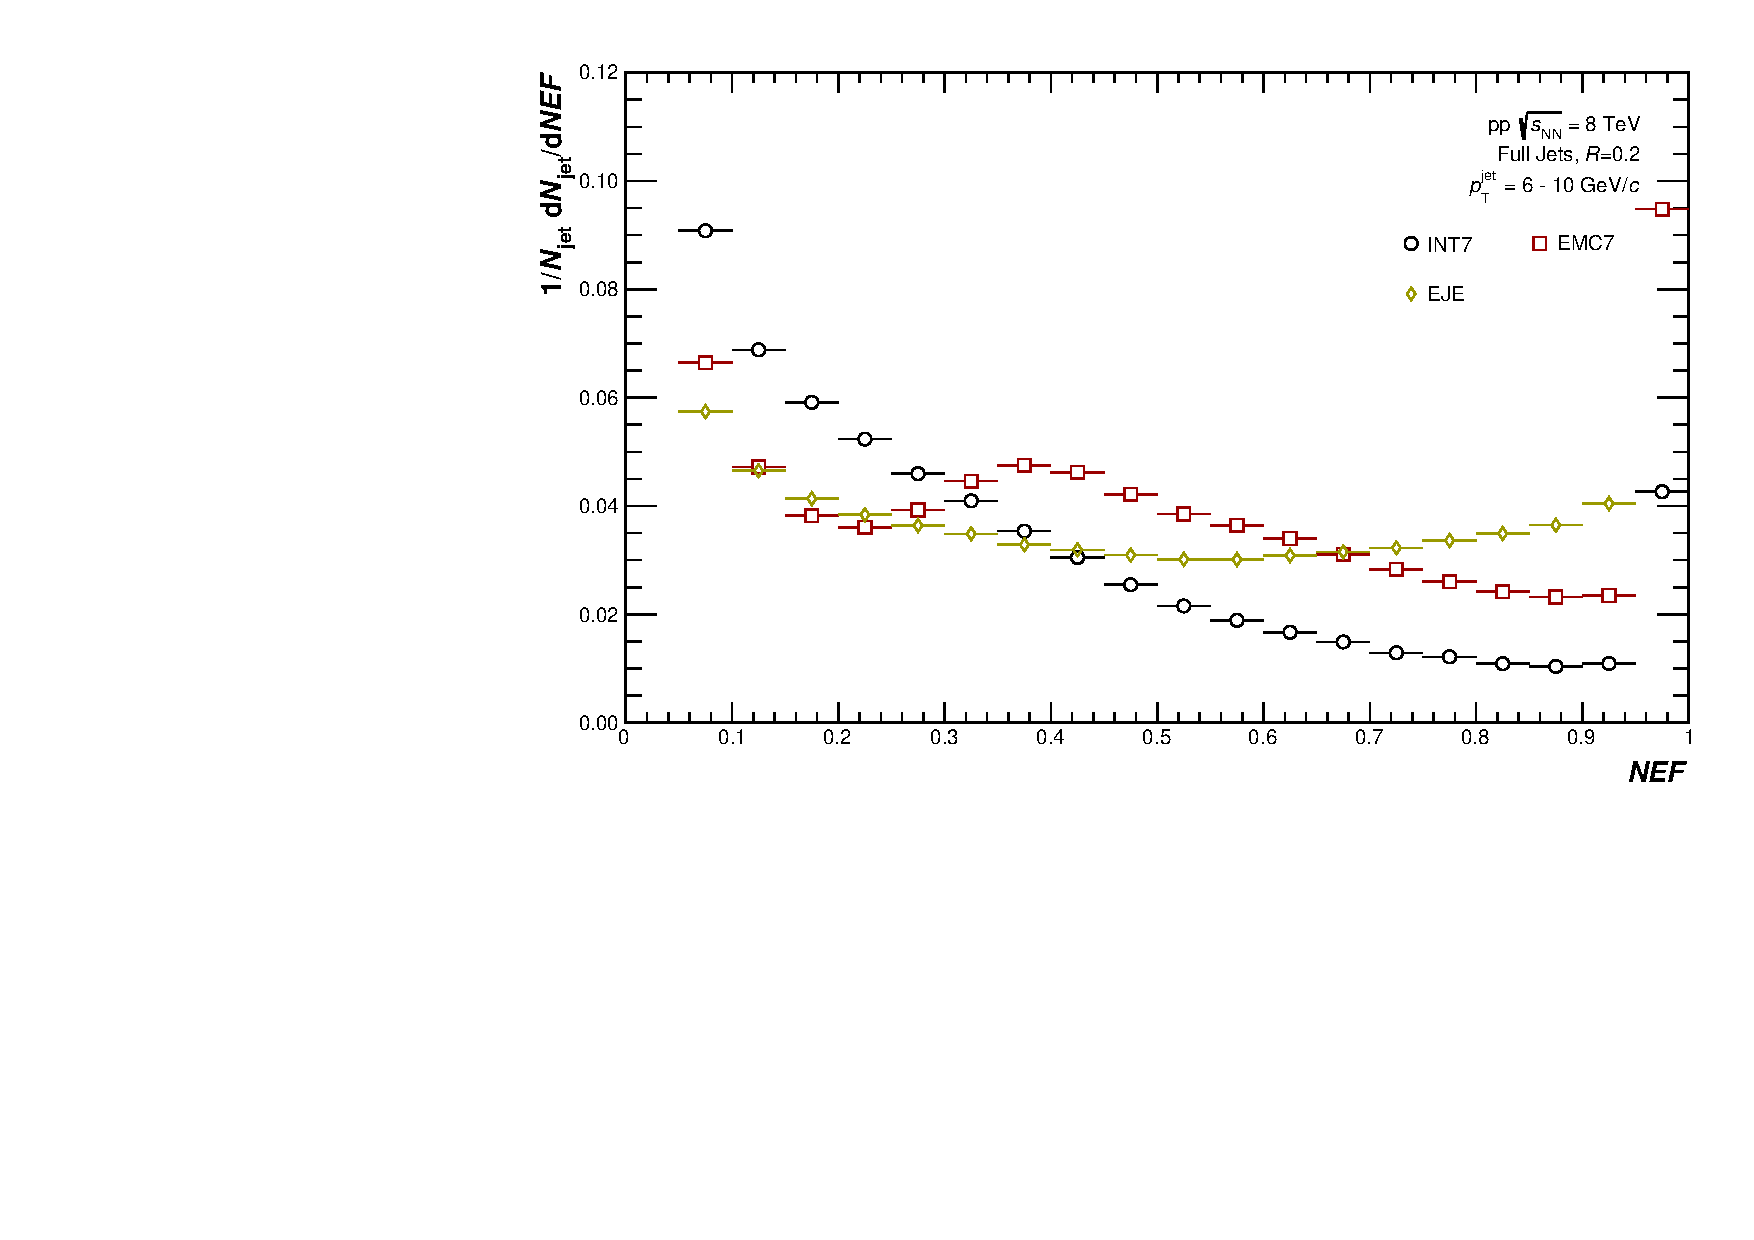
\includegraphics[width=.45\textwidth]{figures/NEF/All/hNEF_6-10GeV_R02.pdf}}
    \qquad
    \subfigure{\label{fig:NEF_10-20GeV_R02}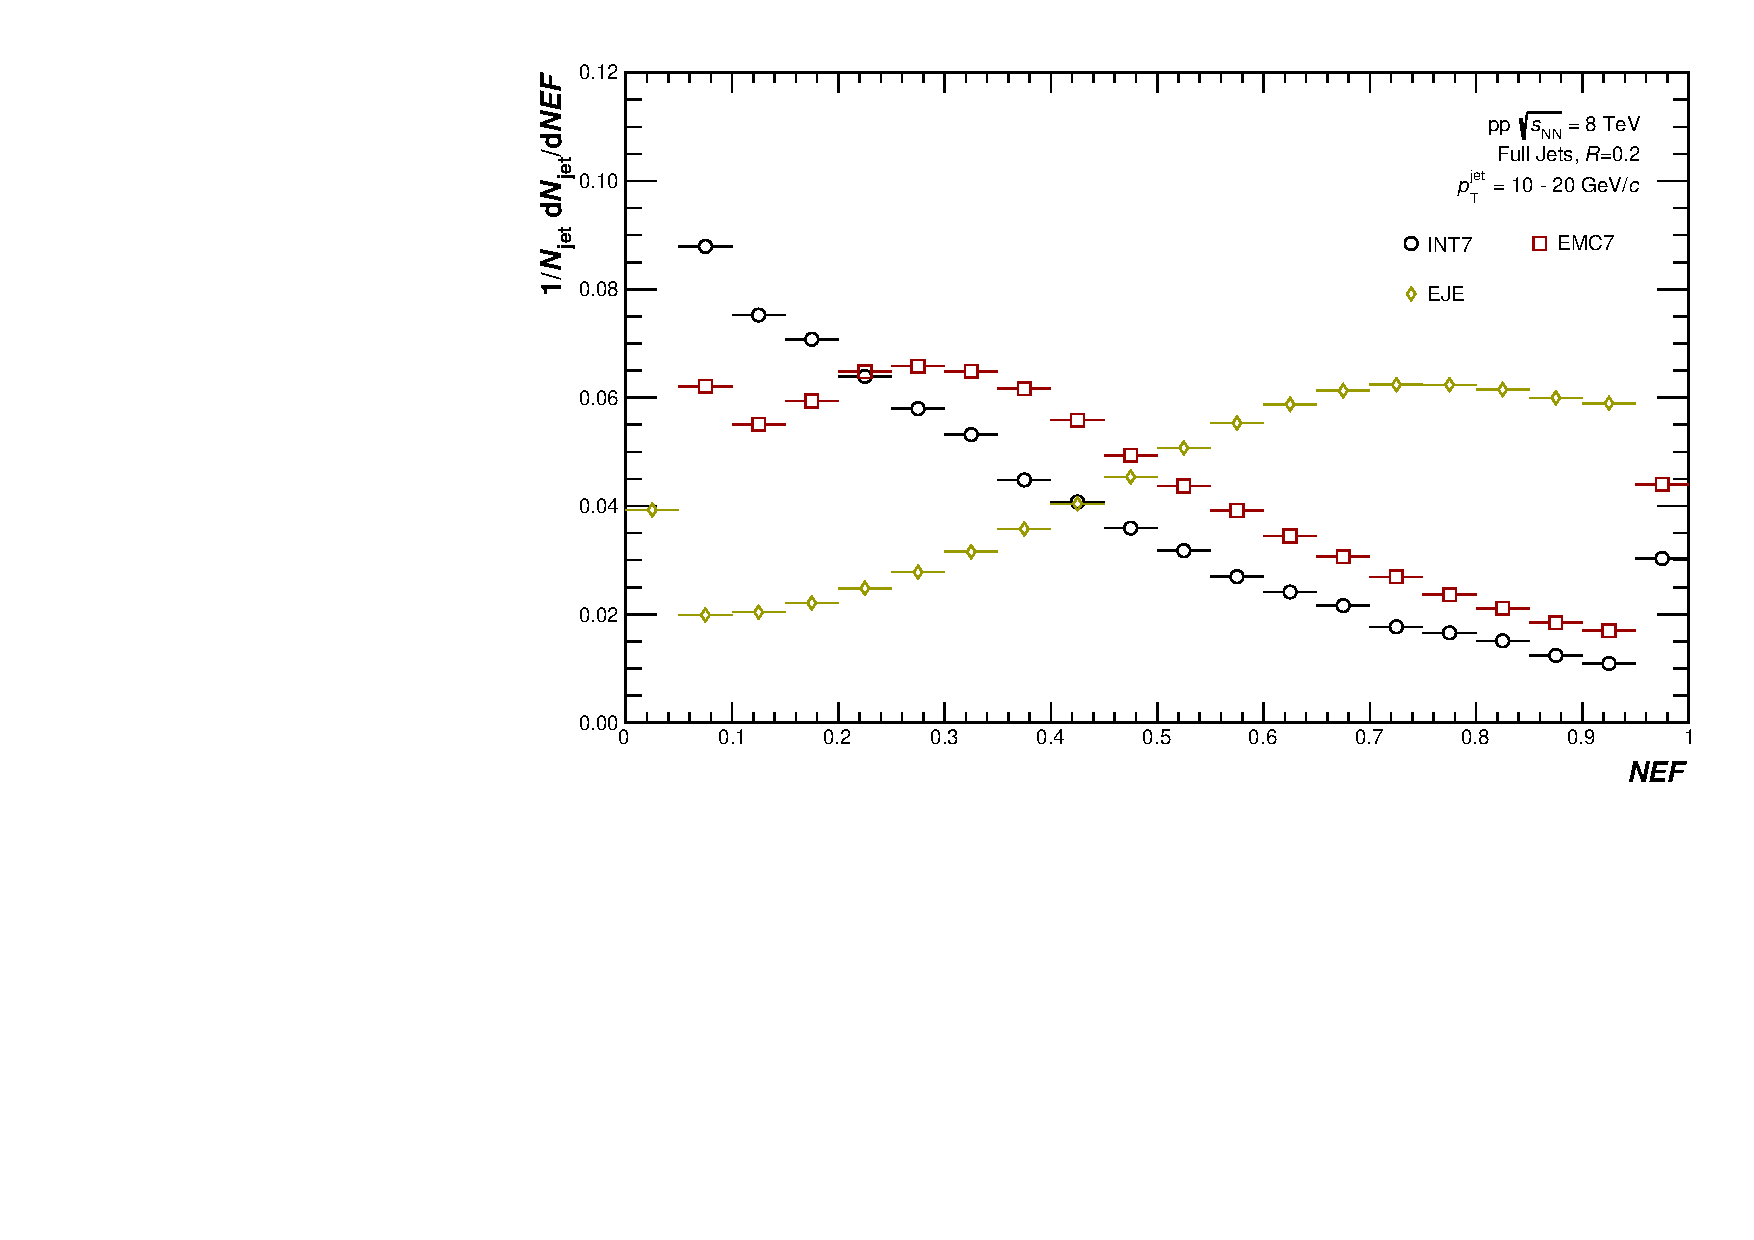
\includegraphics[width=.45\textwidth]{figures/NEF/All/hNEF_10-20GeV_R02.pdf}}\\
    \subfigure{\label{fig:NEF_20-30GeV_R02}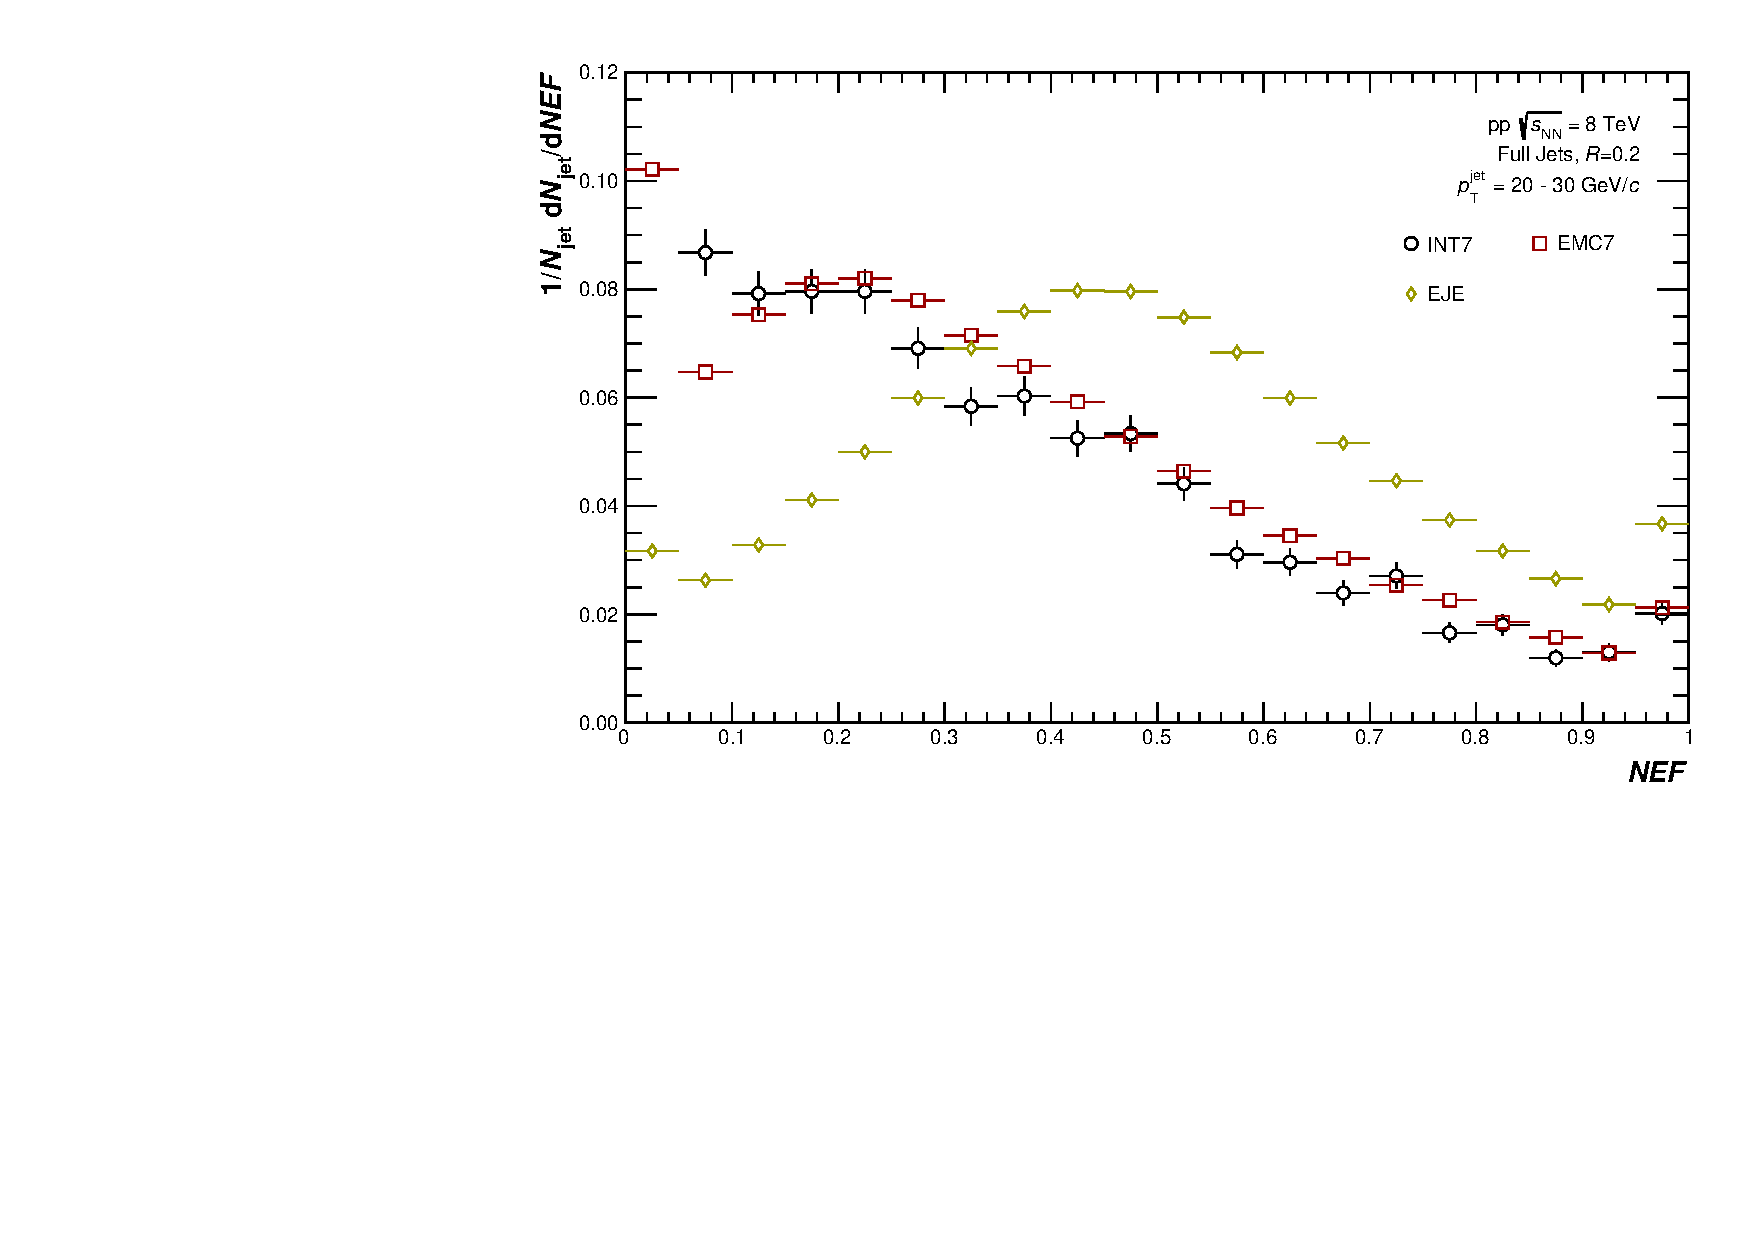
\includegraphics[width=.45\textwidth]{figures/NEF/All/hNEF_20-30GeV_R02.pdf}}
    \qquad
    \subfigure{\label{fig:NEF_30-60GeV_R02}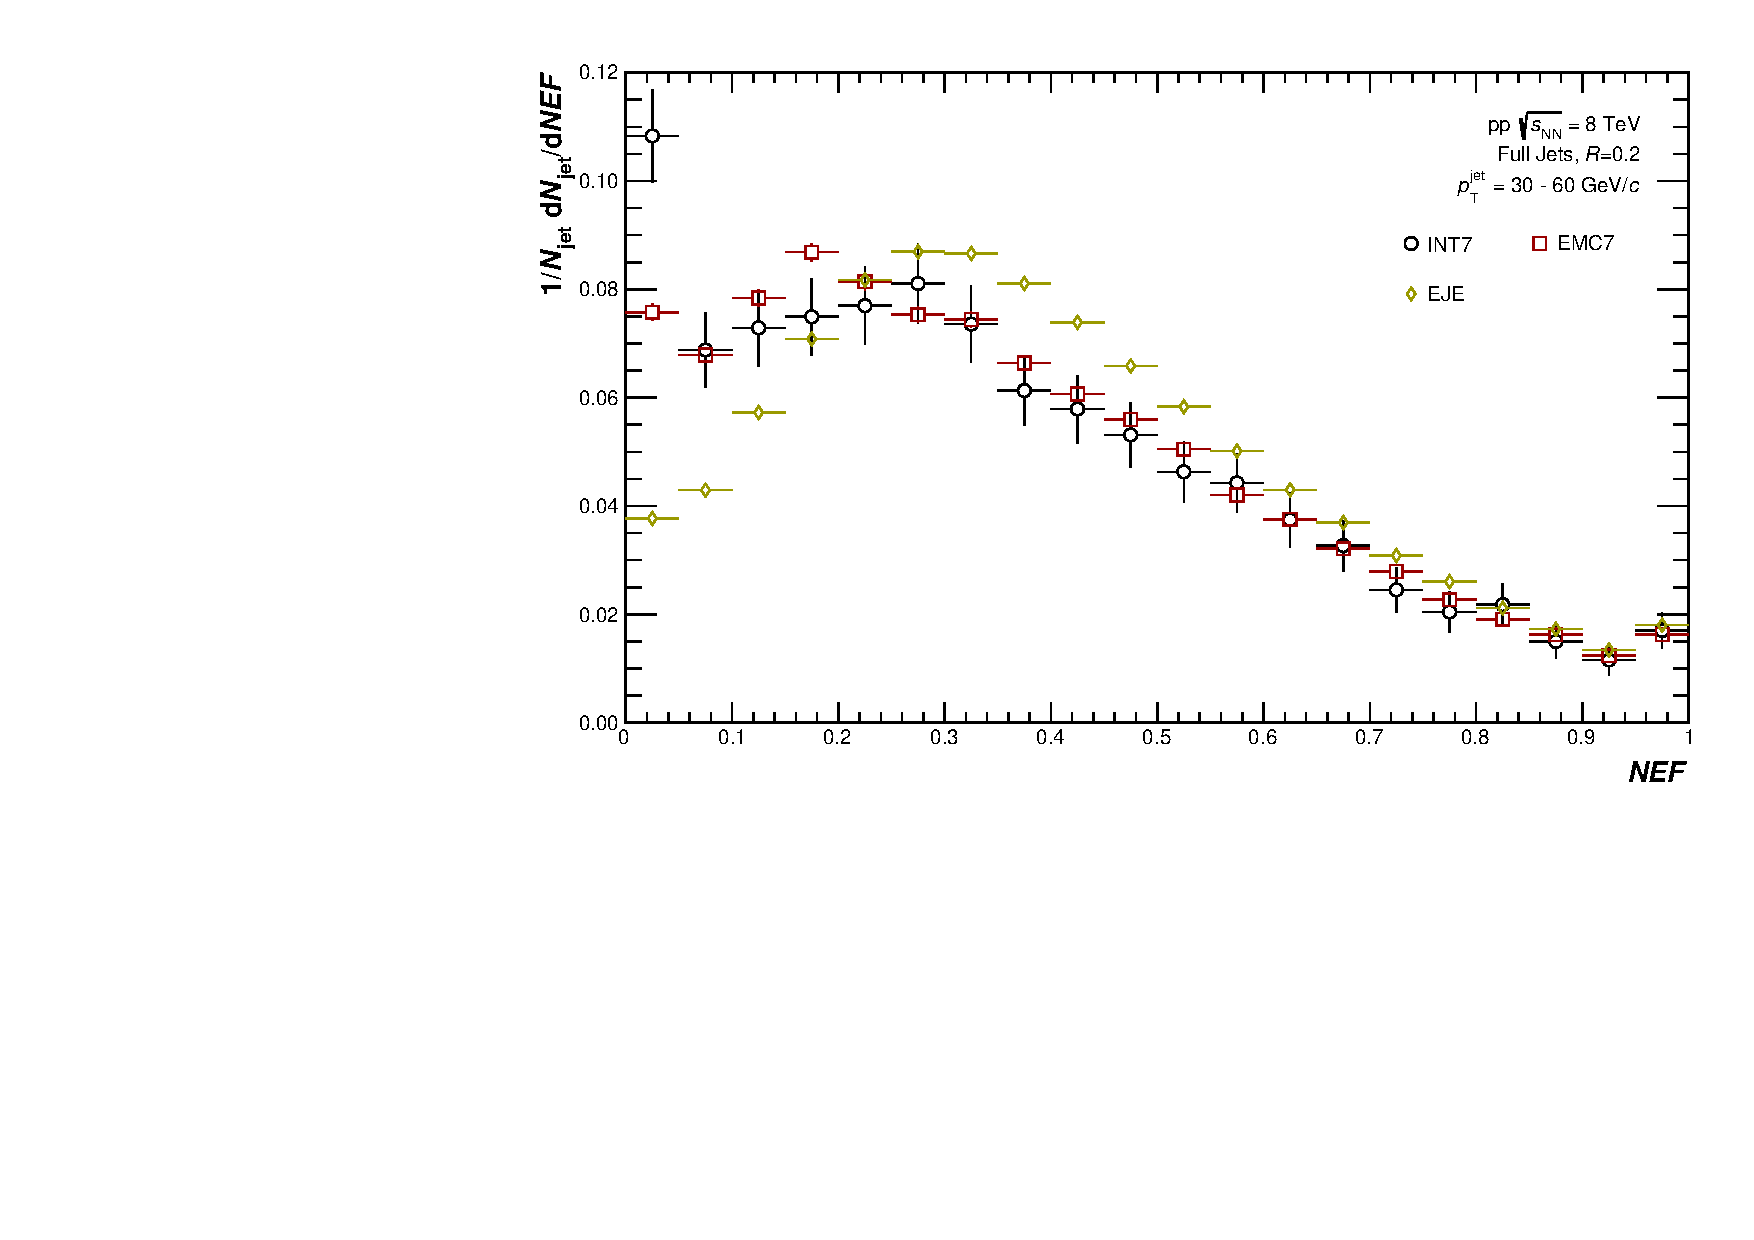
\includegraphics[width=.45\textwidth]{figures/NEF/All/hNEF_30-60GeV_R02.pdf}}\\
    \subfigure{\label{fig:NEF_60-100GeV_R02}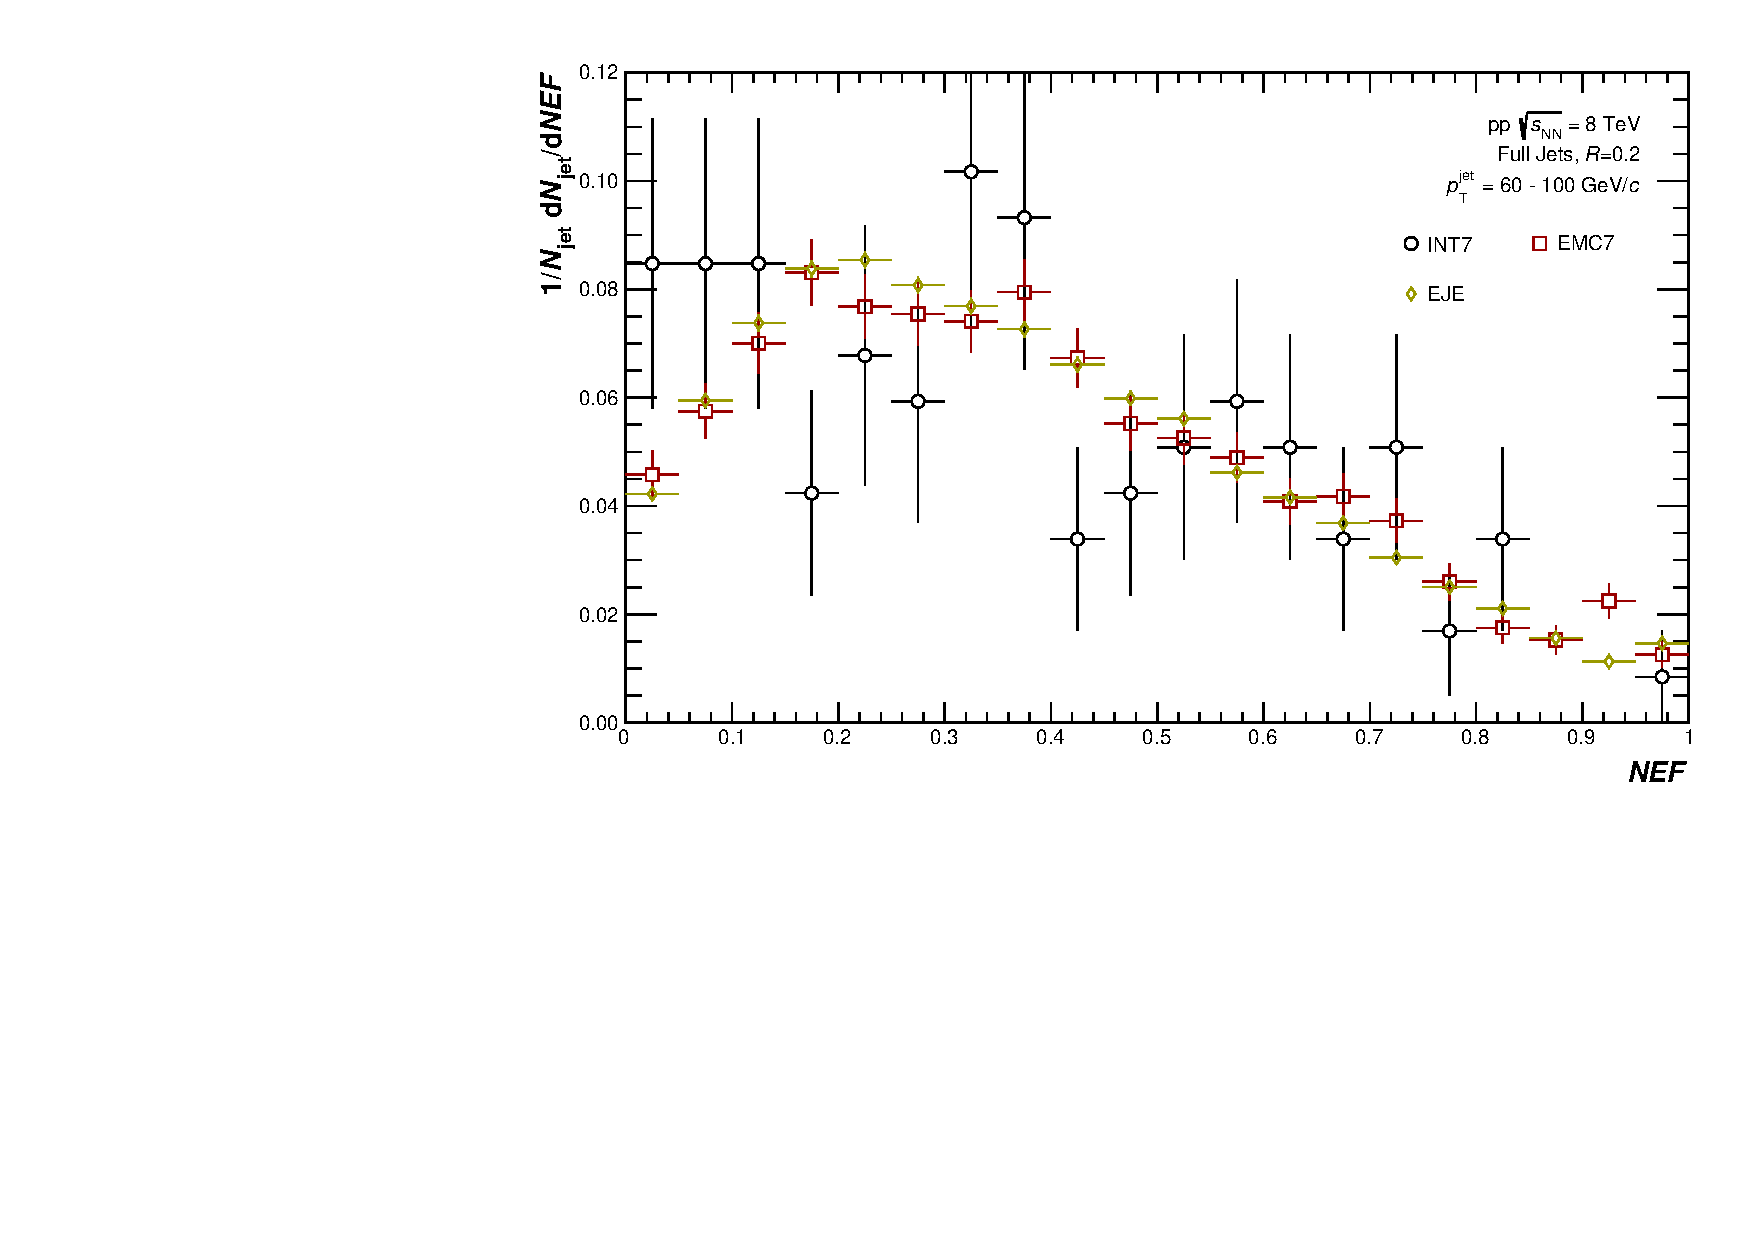
\includegraphics[width=.45\textwidth]{figures/NEF/All/hNEF_60-100GeV_R02.pdf}}
    \qquad
    \subfigure{\label{fig:NEF_100-200GeV_R02}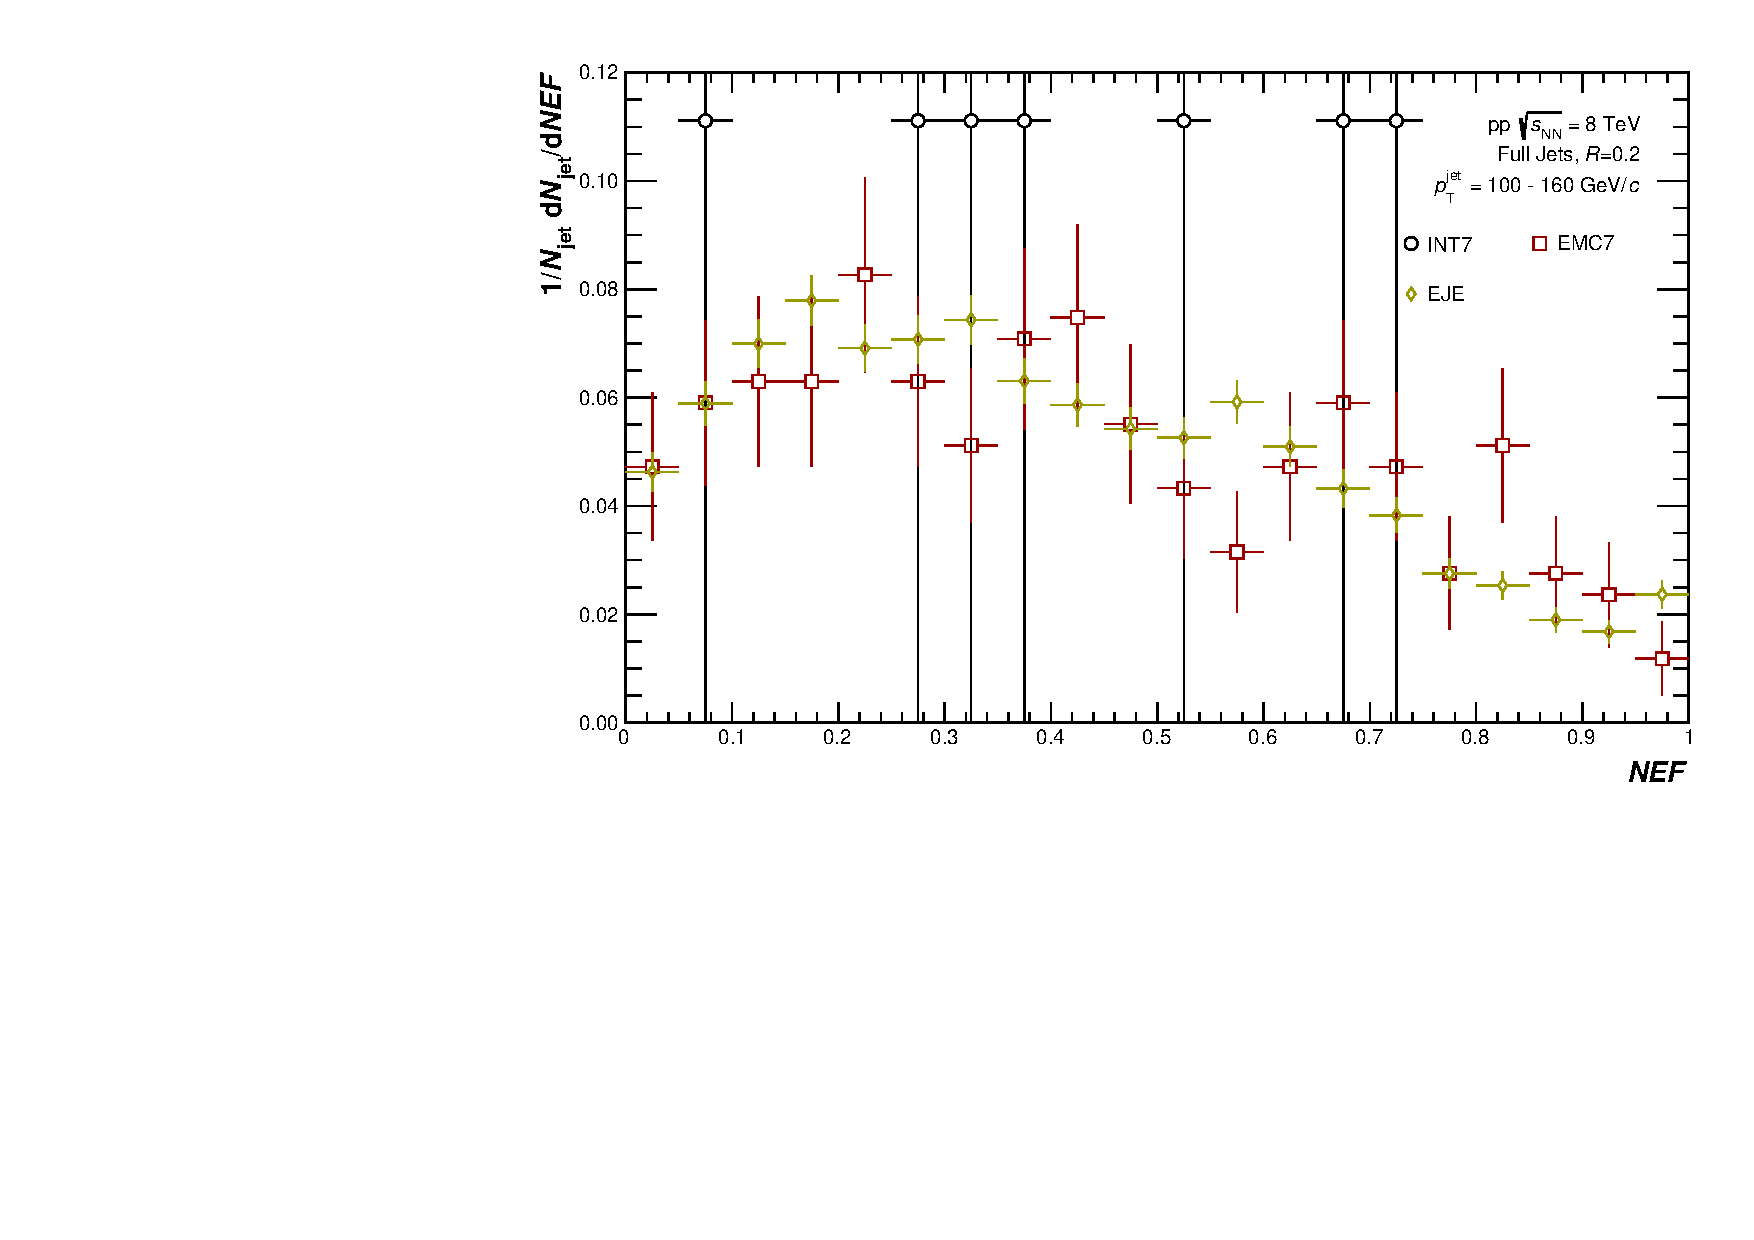
\includegraphics[width=.45\textwidth]{figures/NEF/All/hNEF_100-160GeV_R02.pdf}}\\
    \subfigure{\label{fig:NEF_200-350GeV_R02}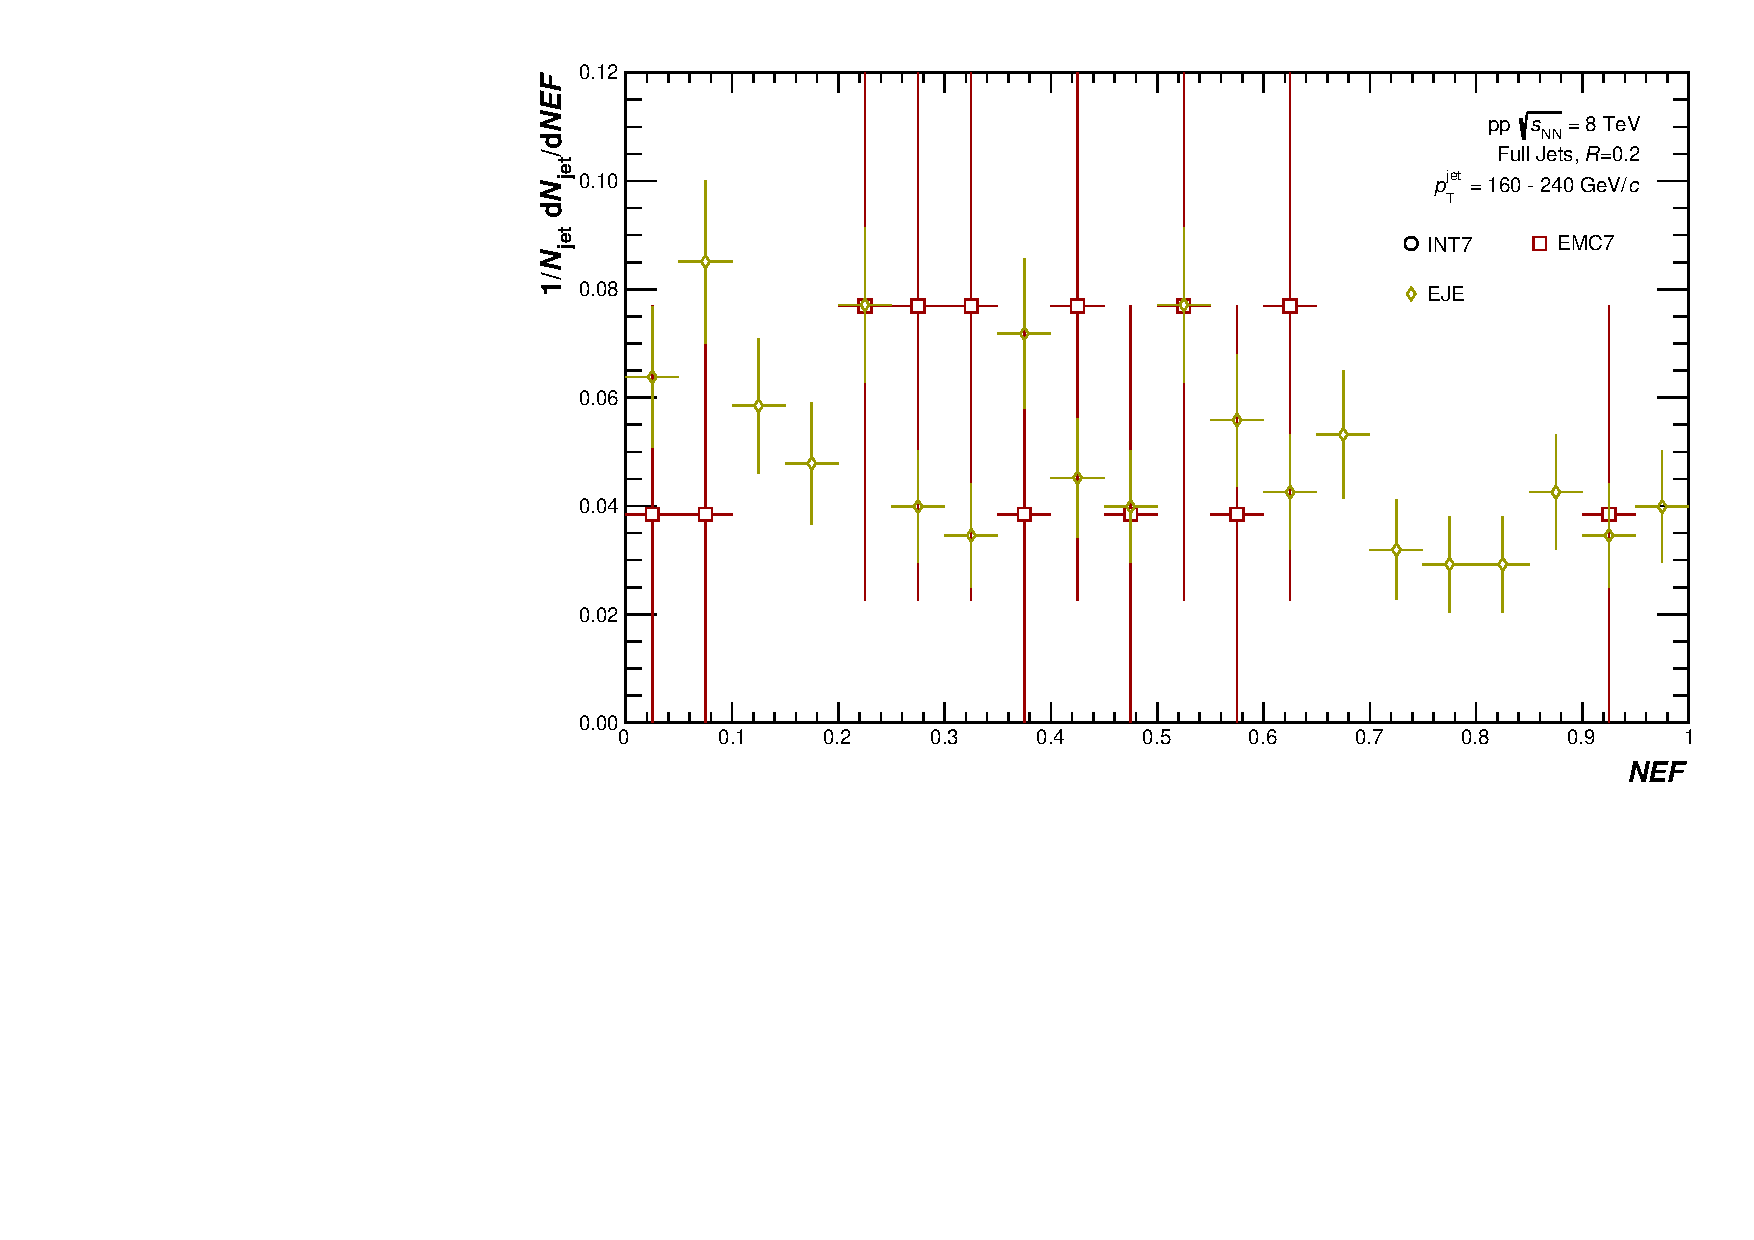
\includegraphics[width=.45\textwidth]{figures/NEF/All/hNEF_160-240GeV_R02.pdf}}
    \caption{NEF for R=0.2 jets in several bins of \pT}
    \label{fig:appendixTriggerBiasNEFR02}
\end{figure}

\newpage

\begin{figure}[h!]
    \centering
    \subfigure{\label{fig:Zch_6-10GeV_R02}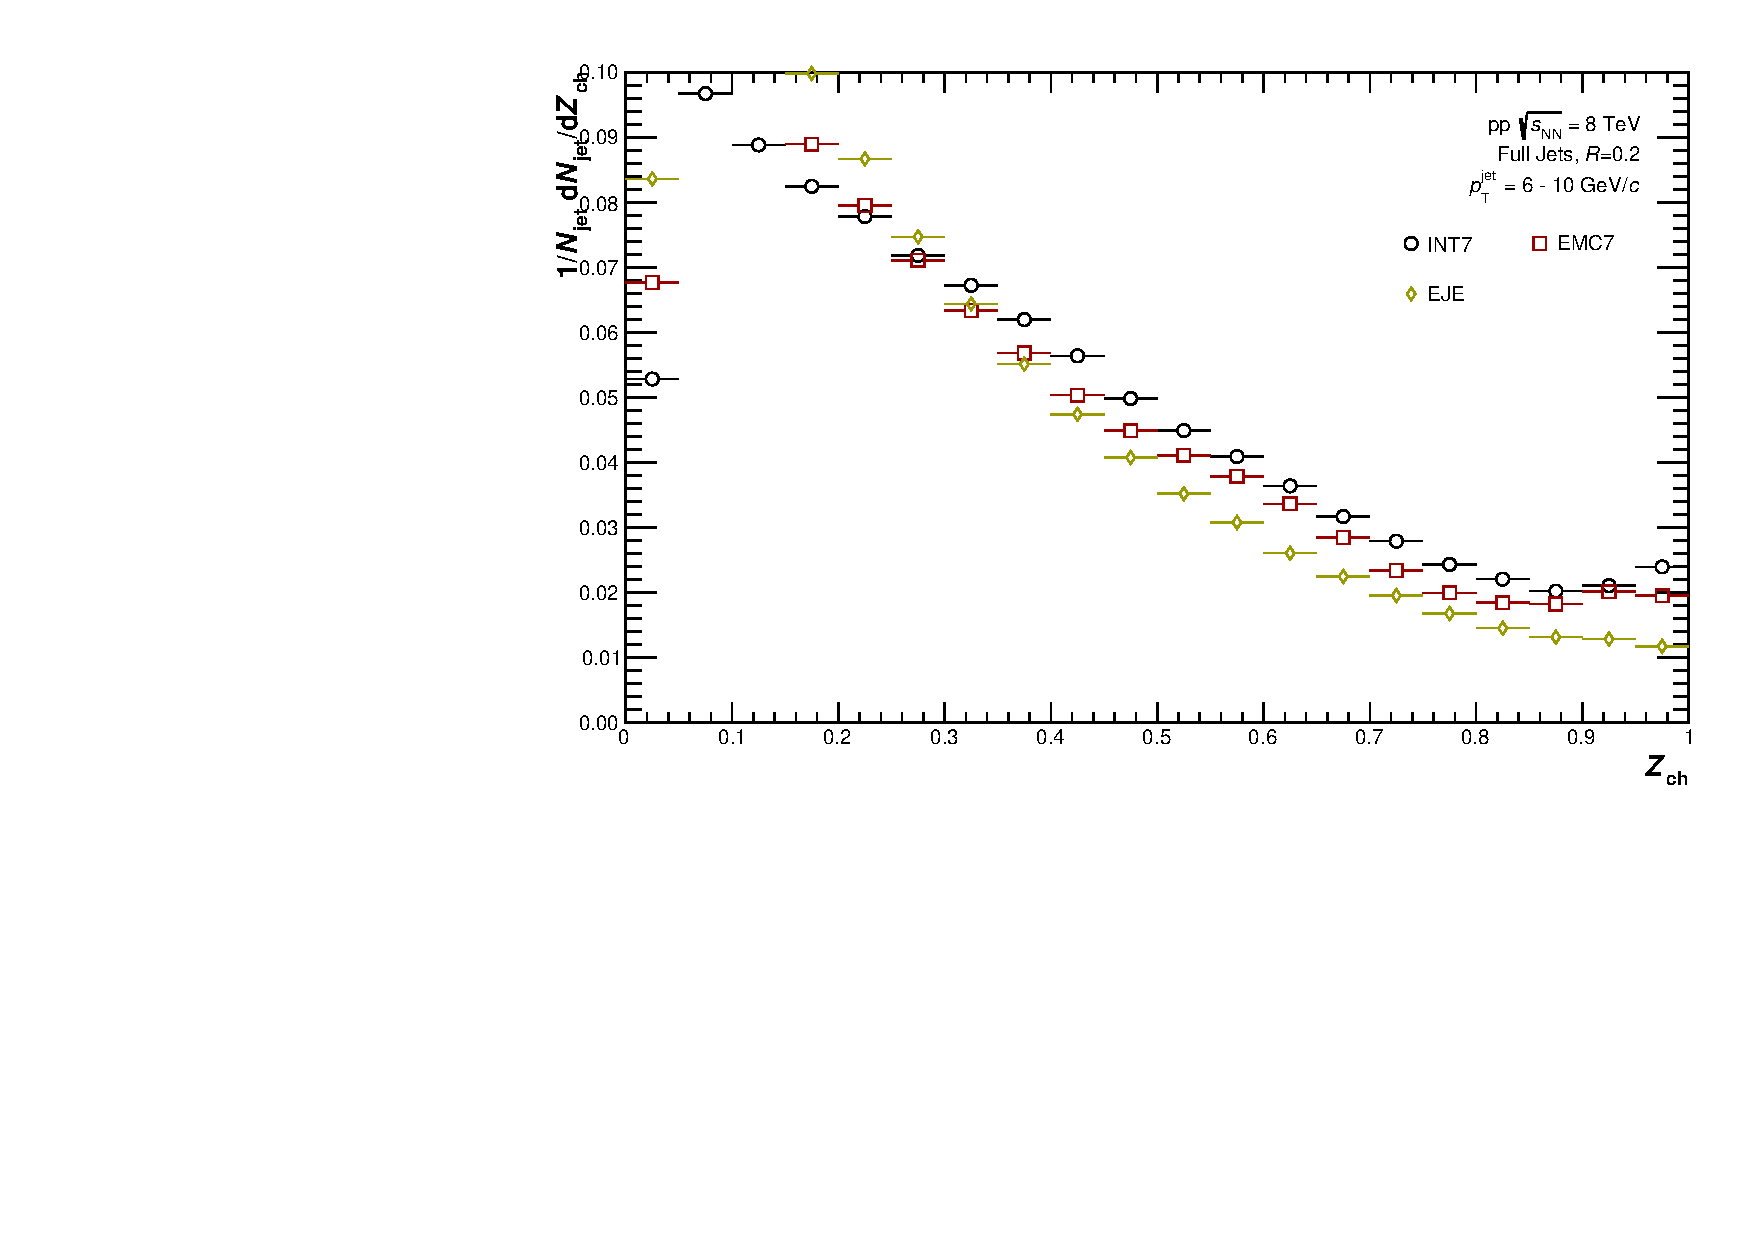
\includegraphics[width=.45\textwidth]{figures/Zch/All/hZch_6-10GeV_R02.pdf}}
    \qquad
    \subfigure{\label{fig:Zch_10-20GeV_R02}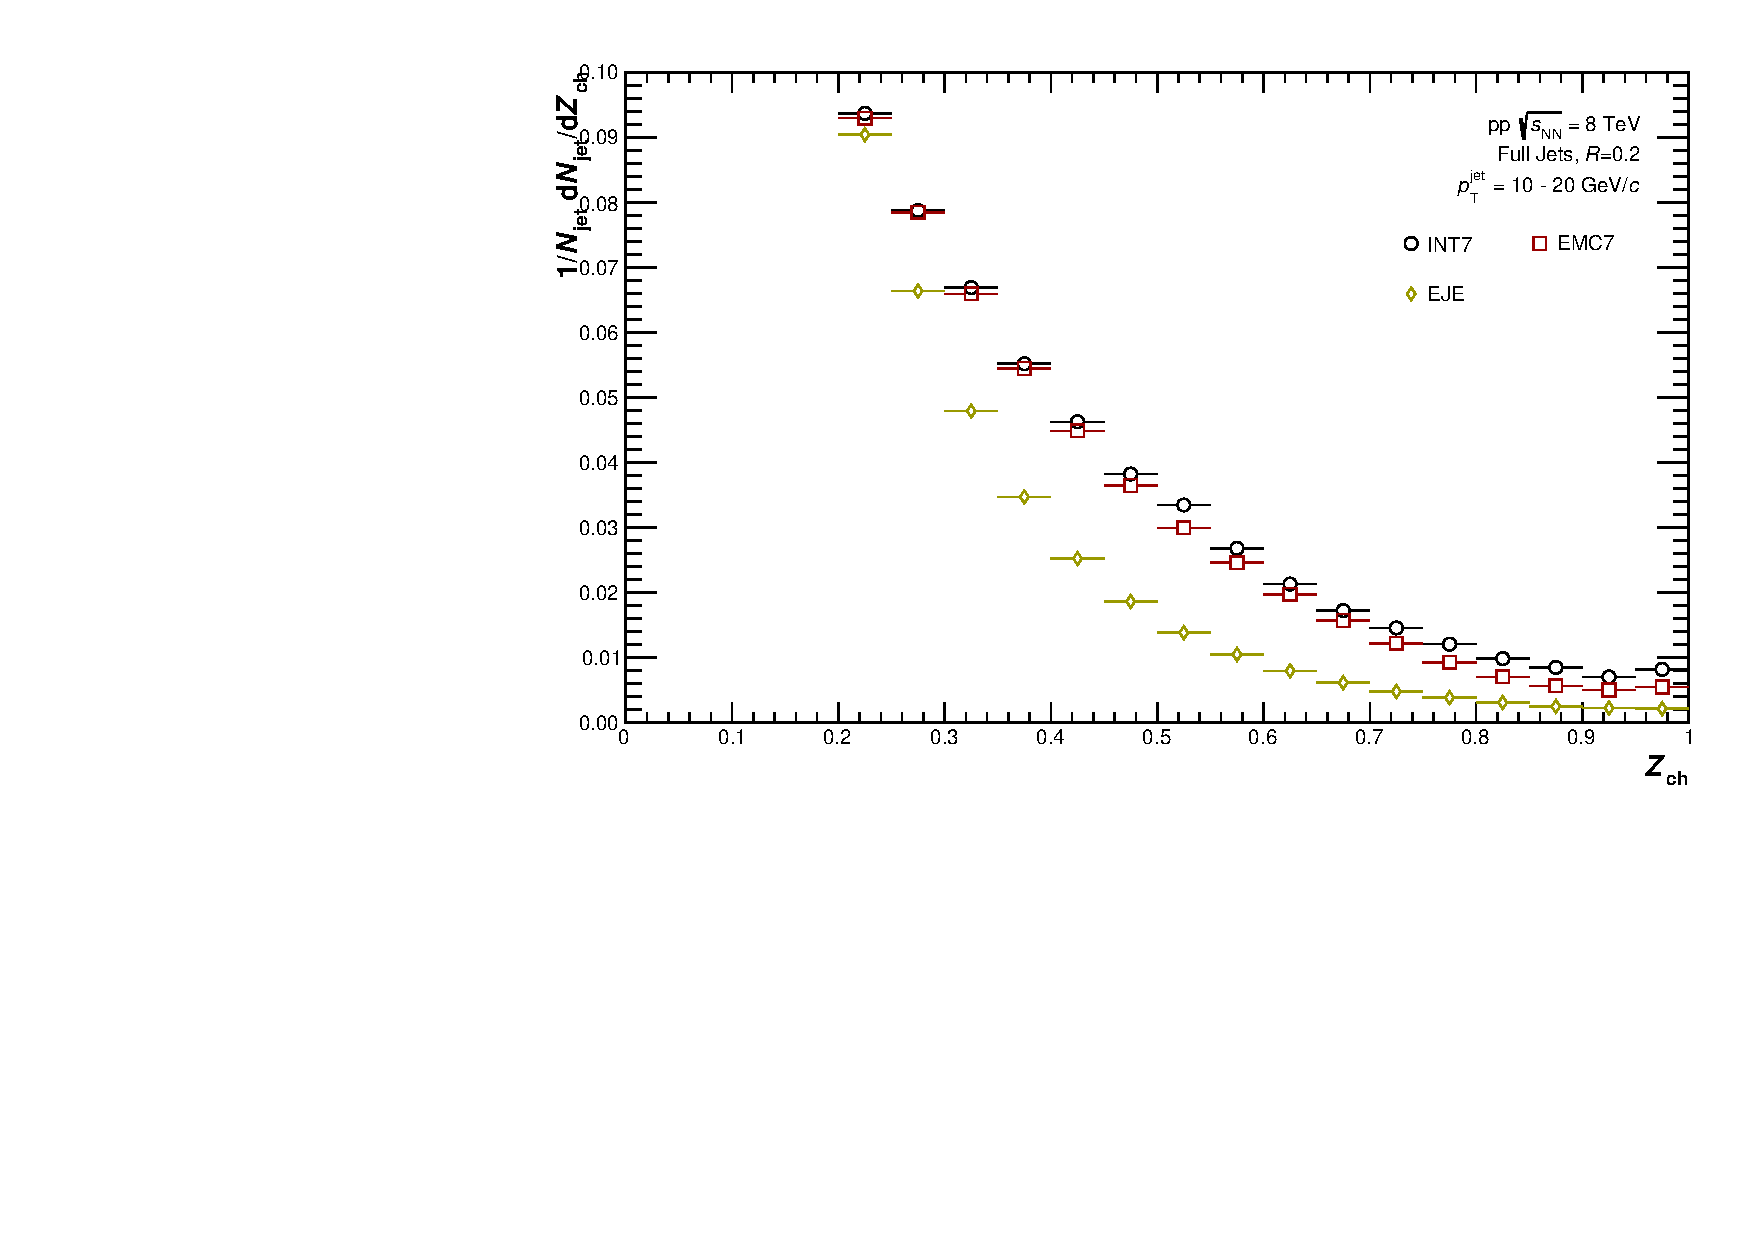
\includegraphics[width=.45\textwidth]{figures/Zch/All/hZch_10-20GeV_R02.pdf}}\\
    \subfigure{\label{fig:Zch_20-30GeV_R02}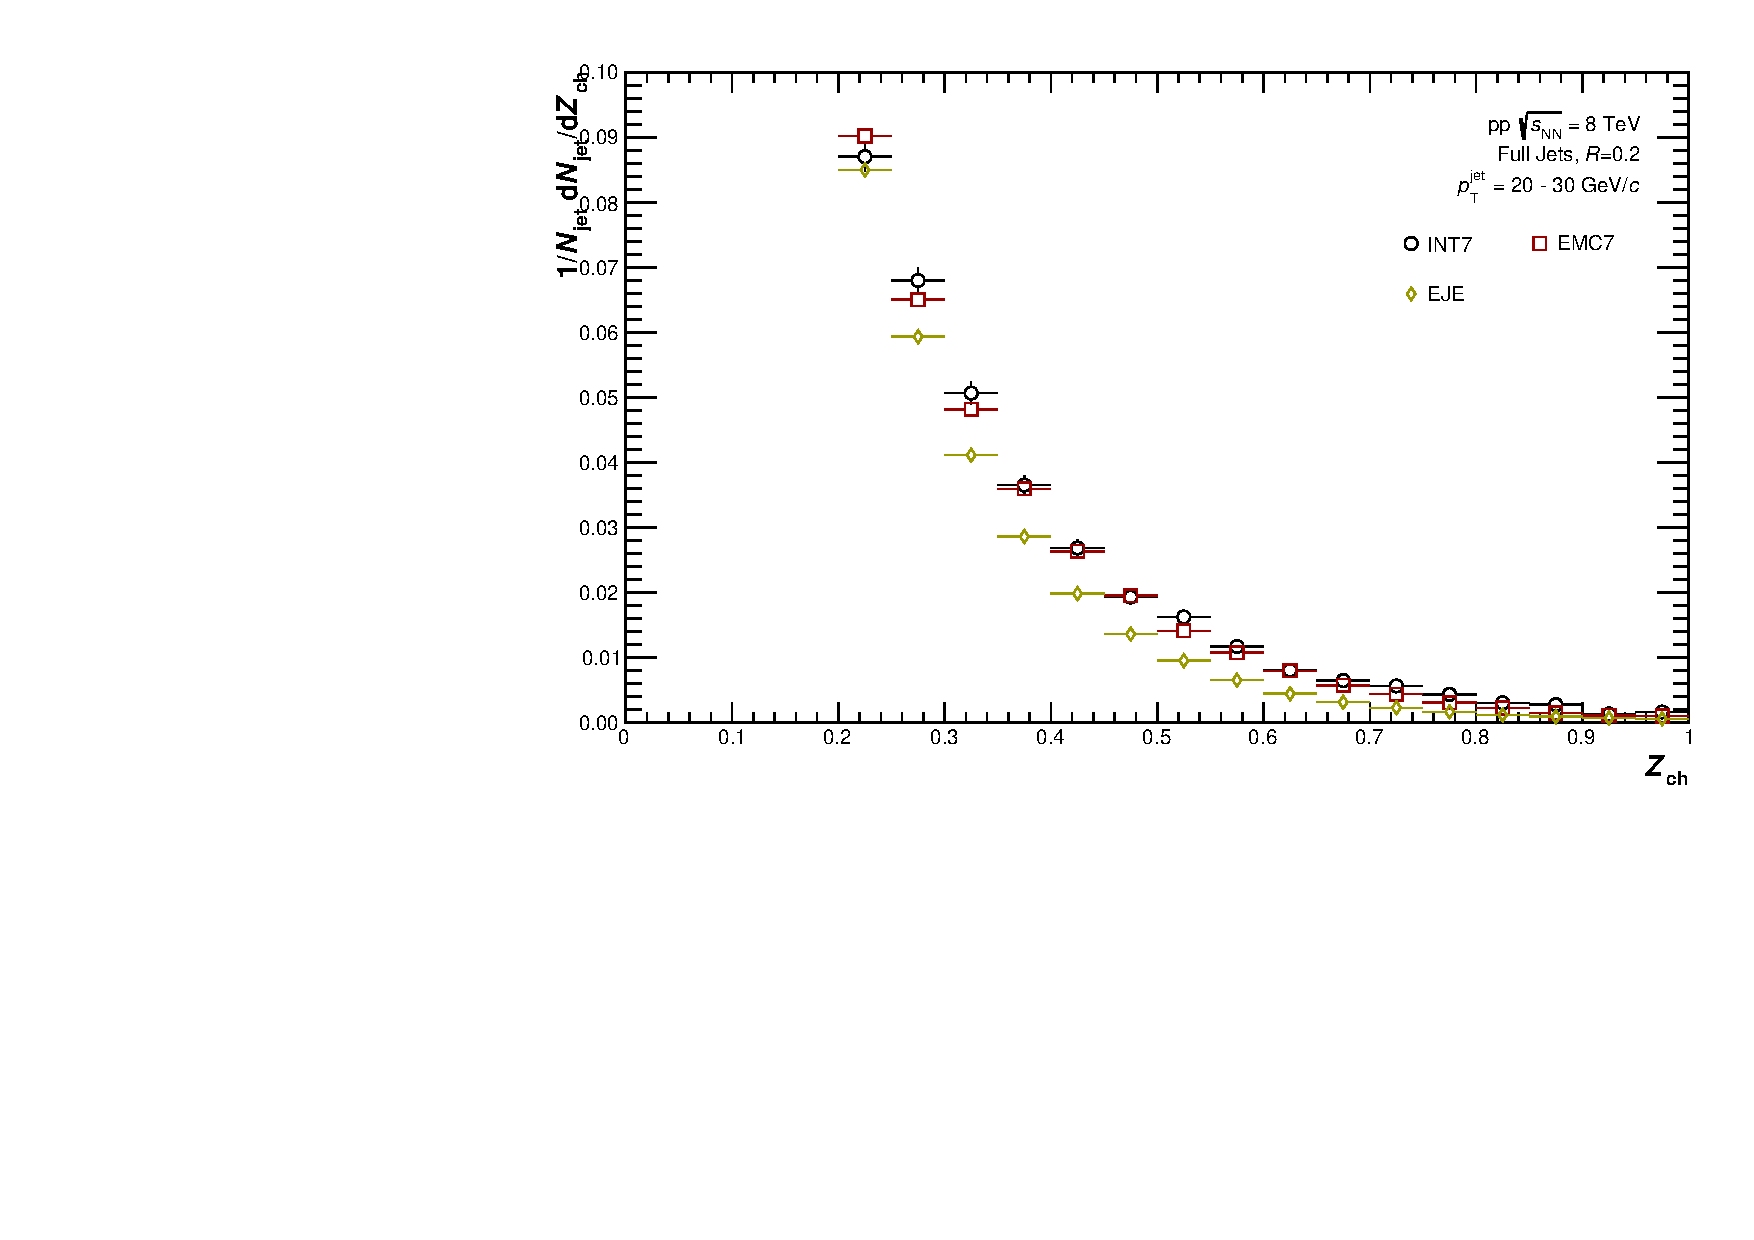
\includegraphics[width=.45\textwidth]{figures/Zch/All/hZch_20-30GeV_R02.pdf}}
    \qquad
    \subfigure{\label{fig:Zch_30-60GeV_R02}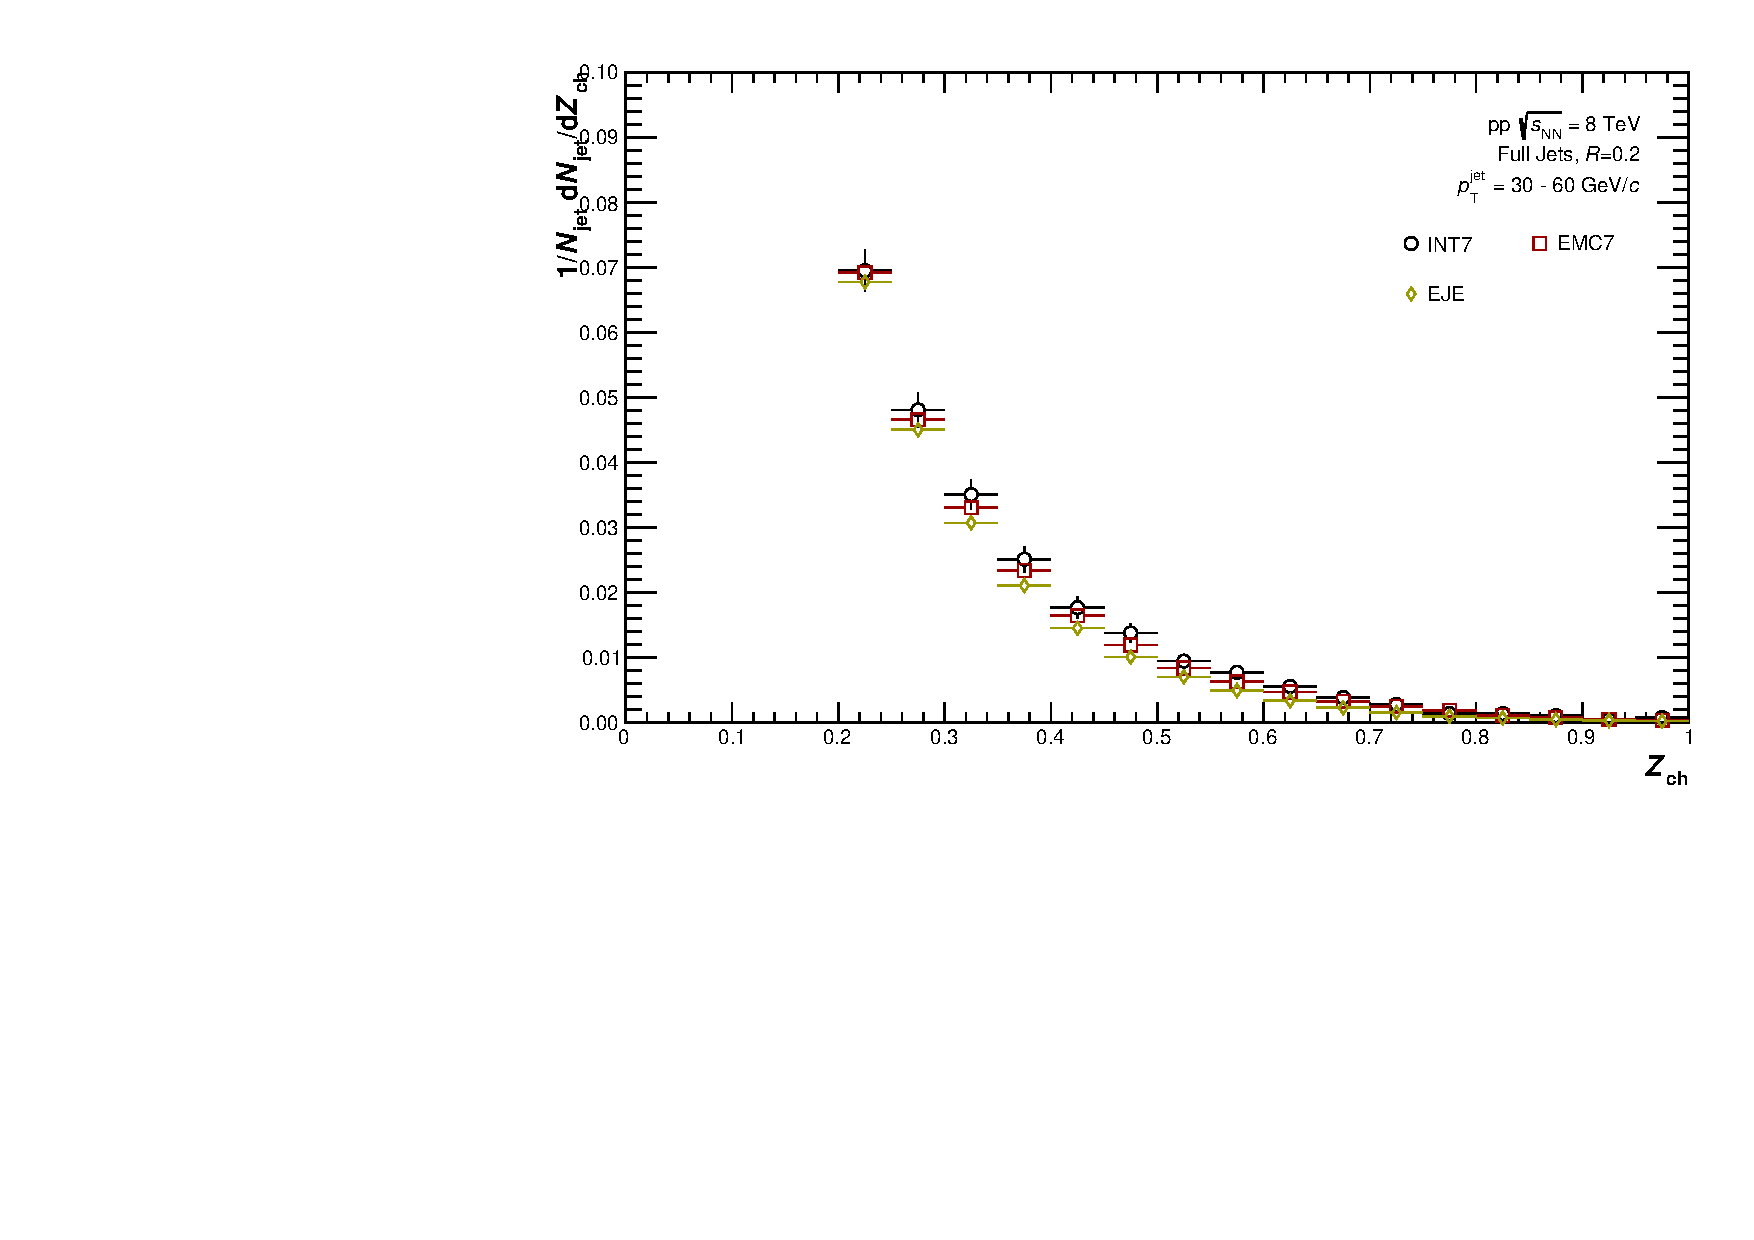
\includegraphics[width=.45\textwidth]{figures/Zch/All/hZch_30-60GeV_R02.pdf}}\\
    \subfigure{\label{fig:Zch_60-100GeV_R02}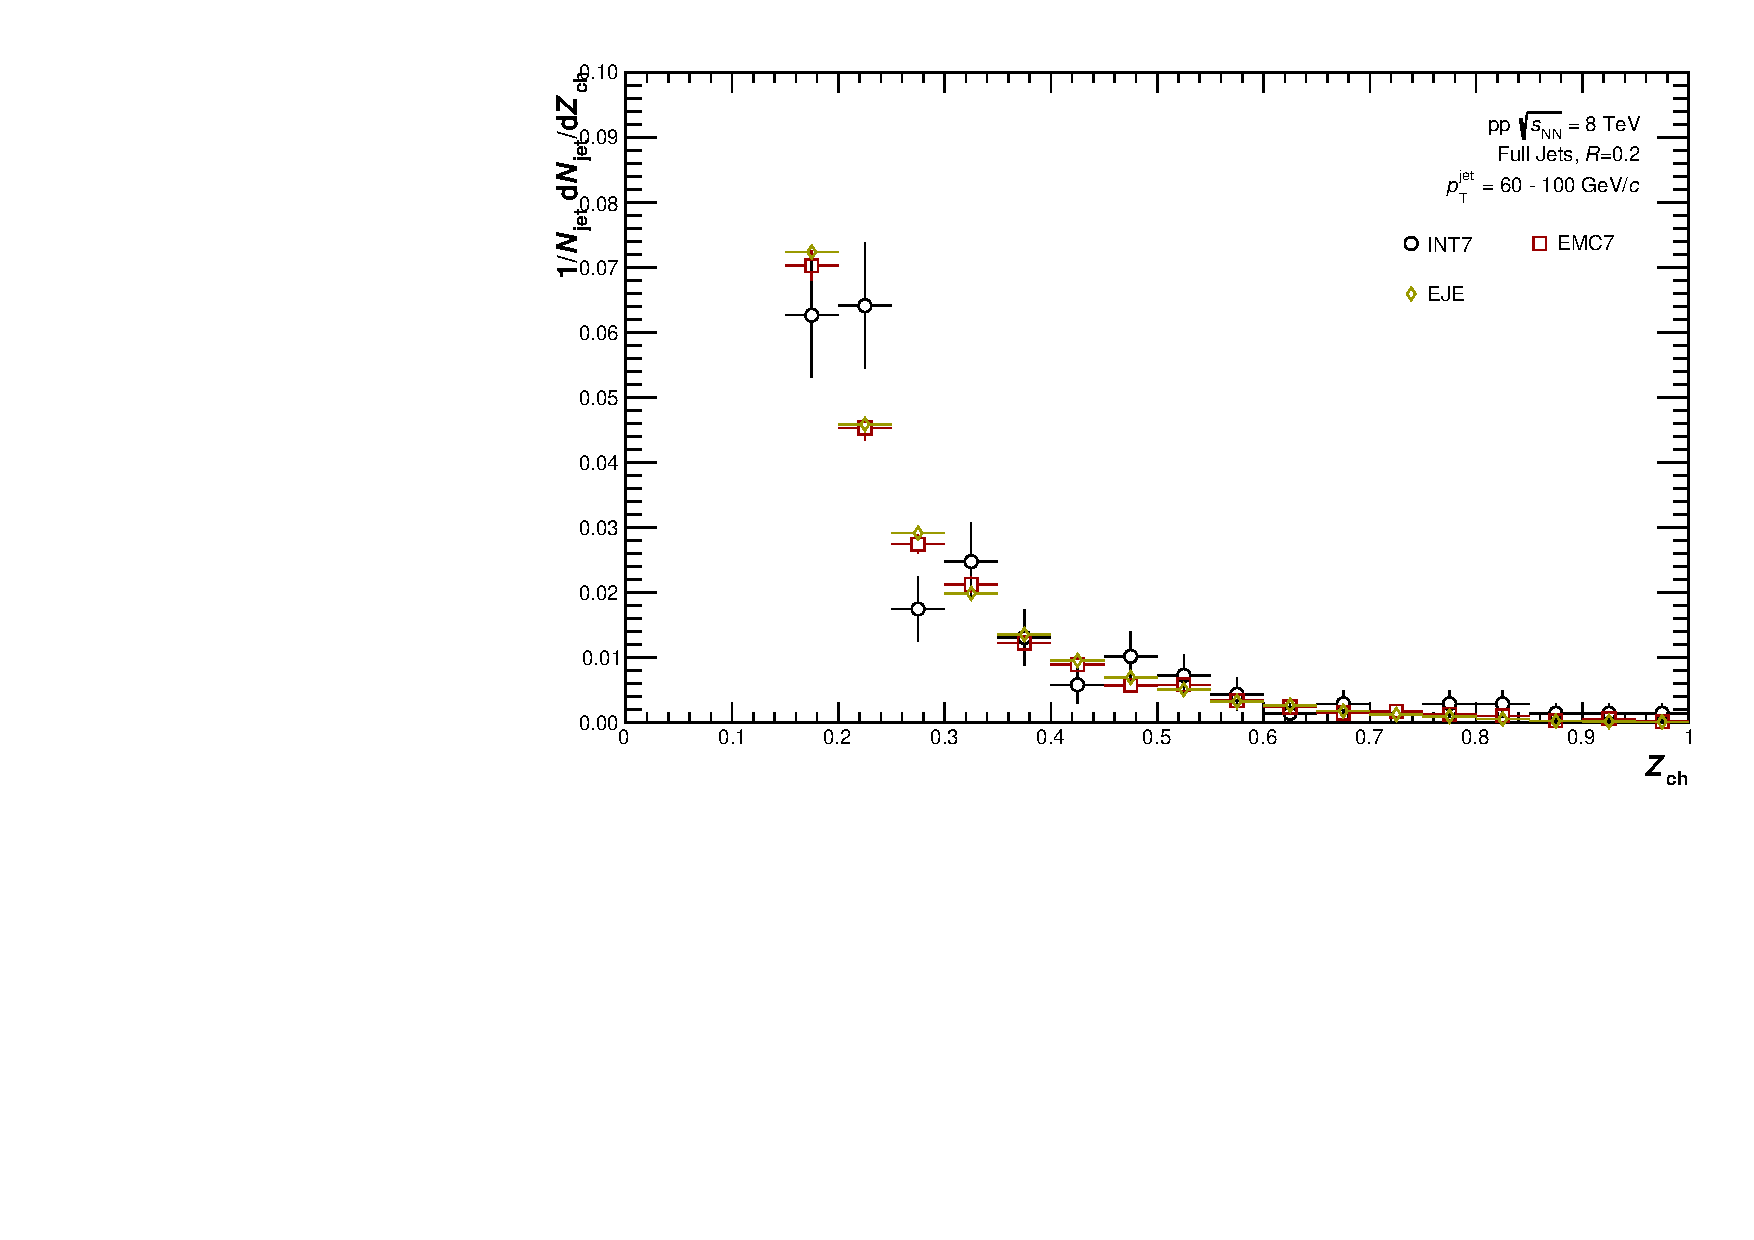
\includegraphics[width=.45\textwidth]{figures/Zch/All/hZch_60-100GeV_R02.pdf}}
    \qquad
    \subfigure{\label{fig:Zch_100-200GeV_R02}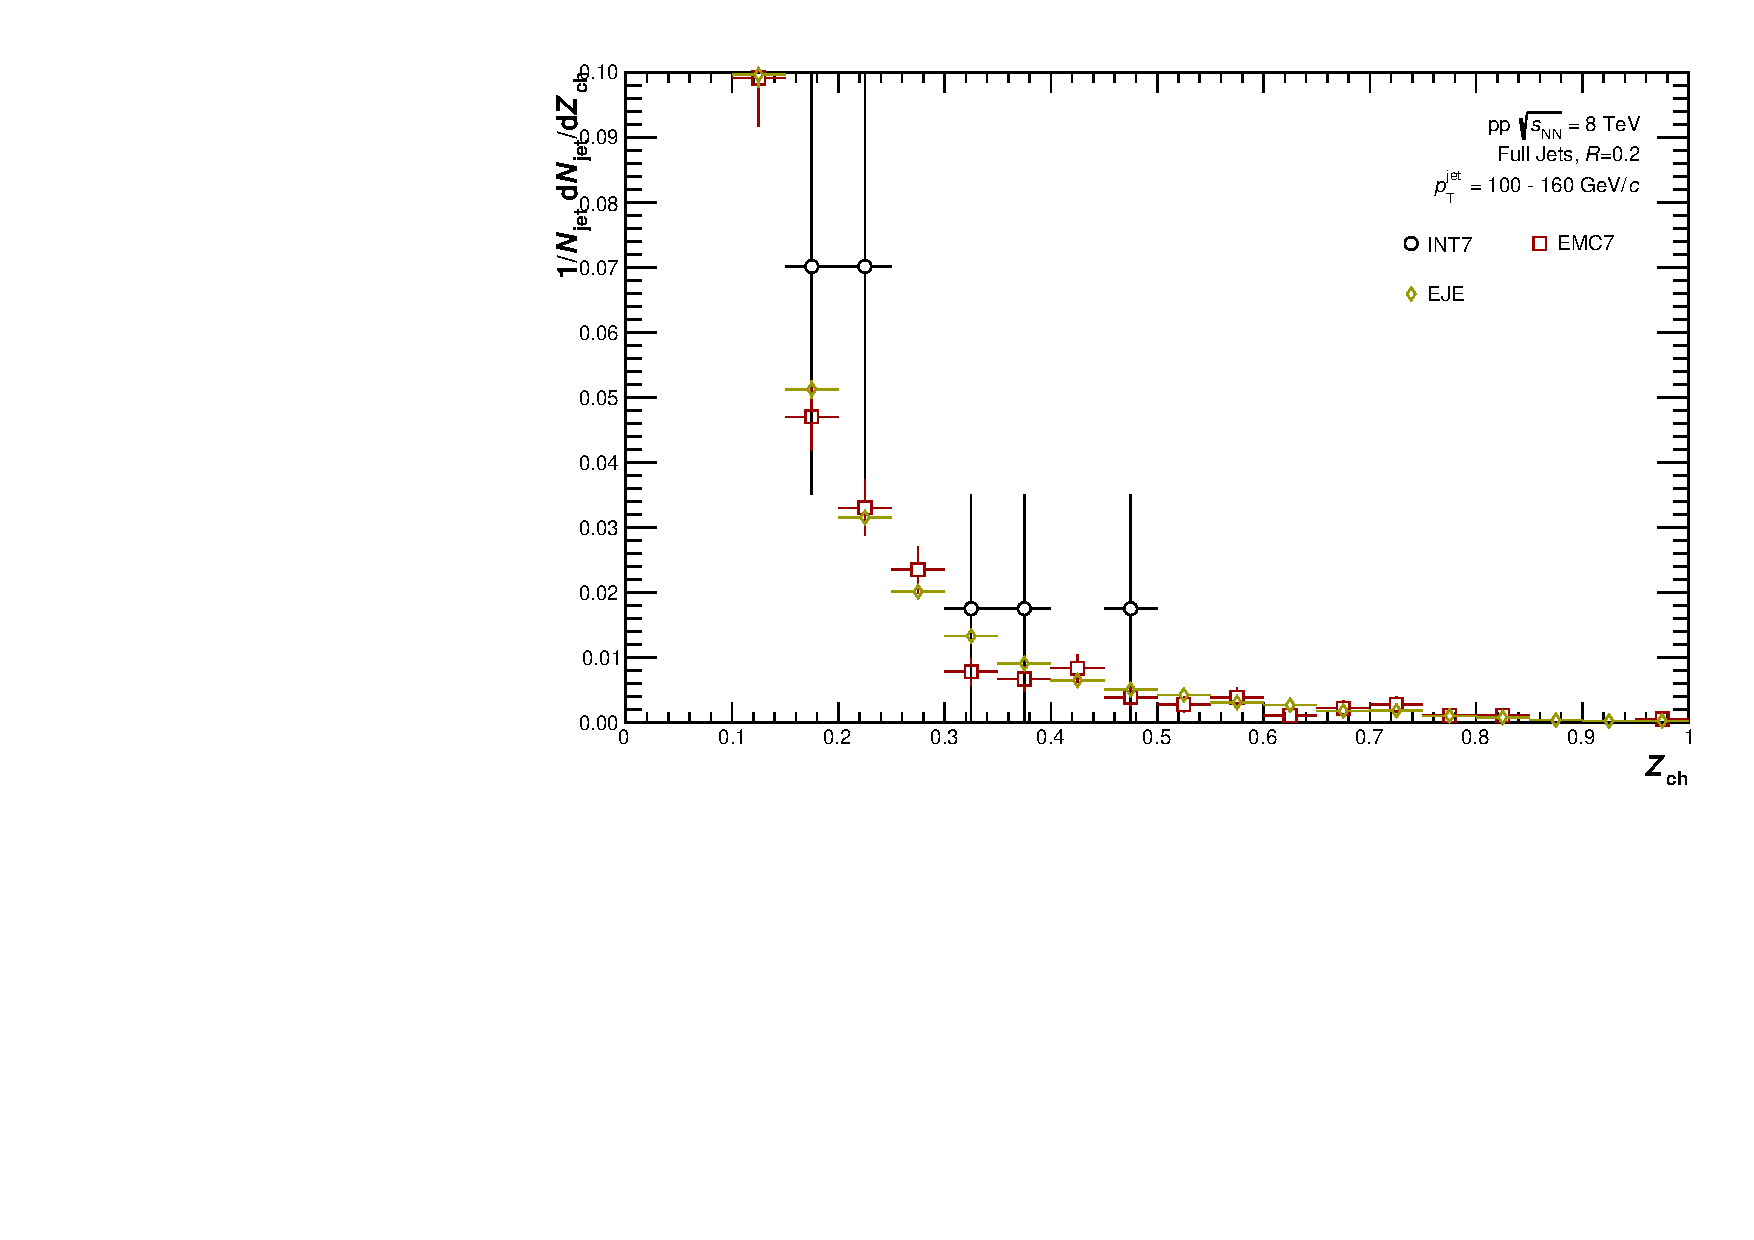
\includegraphics[width=.45\textwidth]{figures/Zch/All/hZch_100-160GeV_R02.pdf}}\\
    \subfigure{\label{fig:Zch_200-350GeV_R02}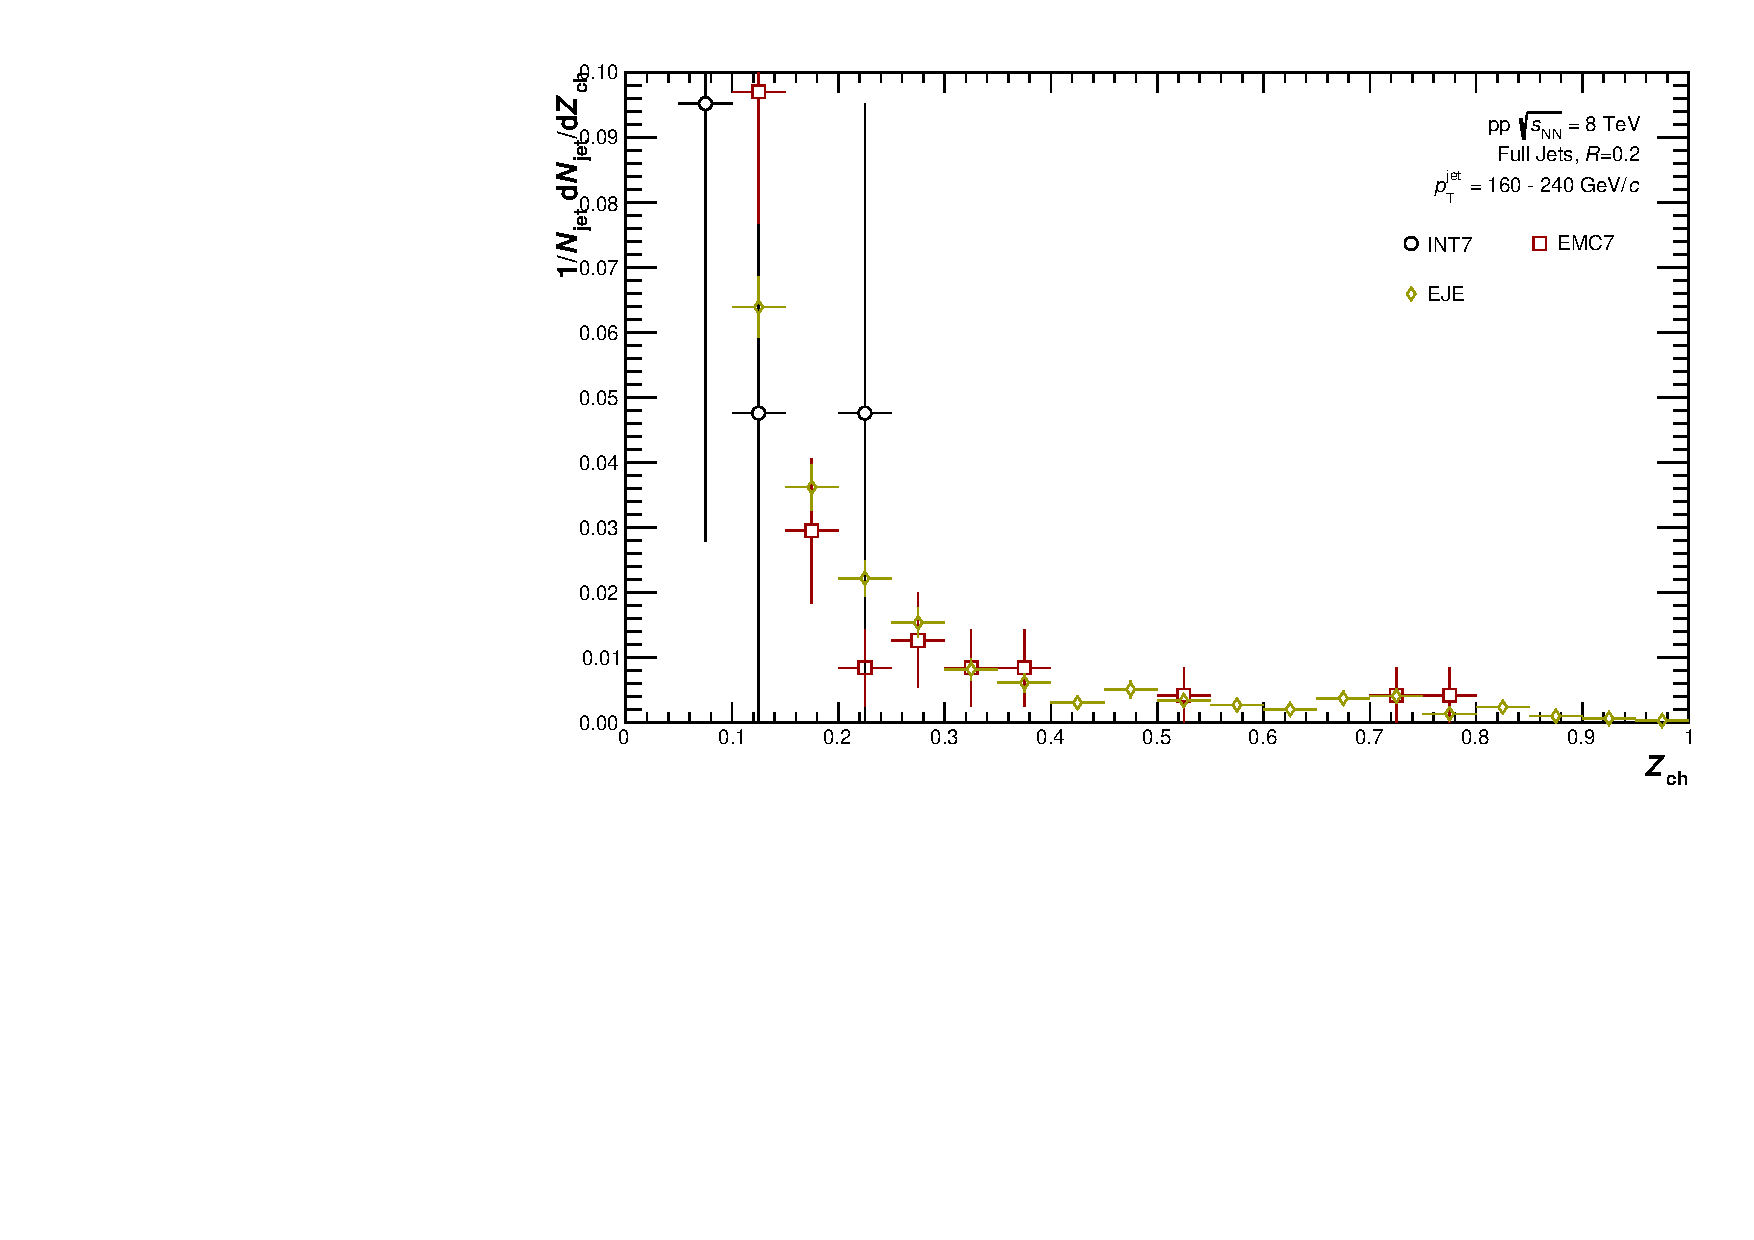
\includegraphics[width=.45\textwidth]{figures/Zch/All/hZch_160-240GeV_R02.pdf}}
    \caption{Z$_{ch}$ for R=0.2 jets in several bins of \pT}
    \label{fig:TriggerBiasZchR02}
\end{figure}

\newpage

\begin{figure}[h!]
    \centering
    \subfigure{\label{fig:Zne_6-10GeV_R02}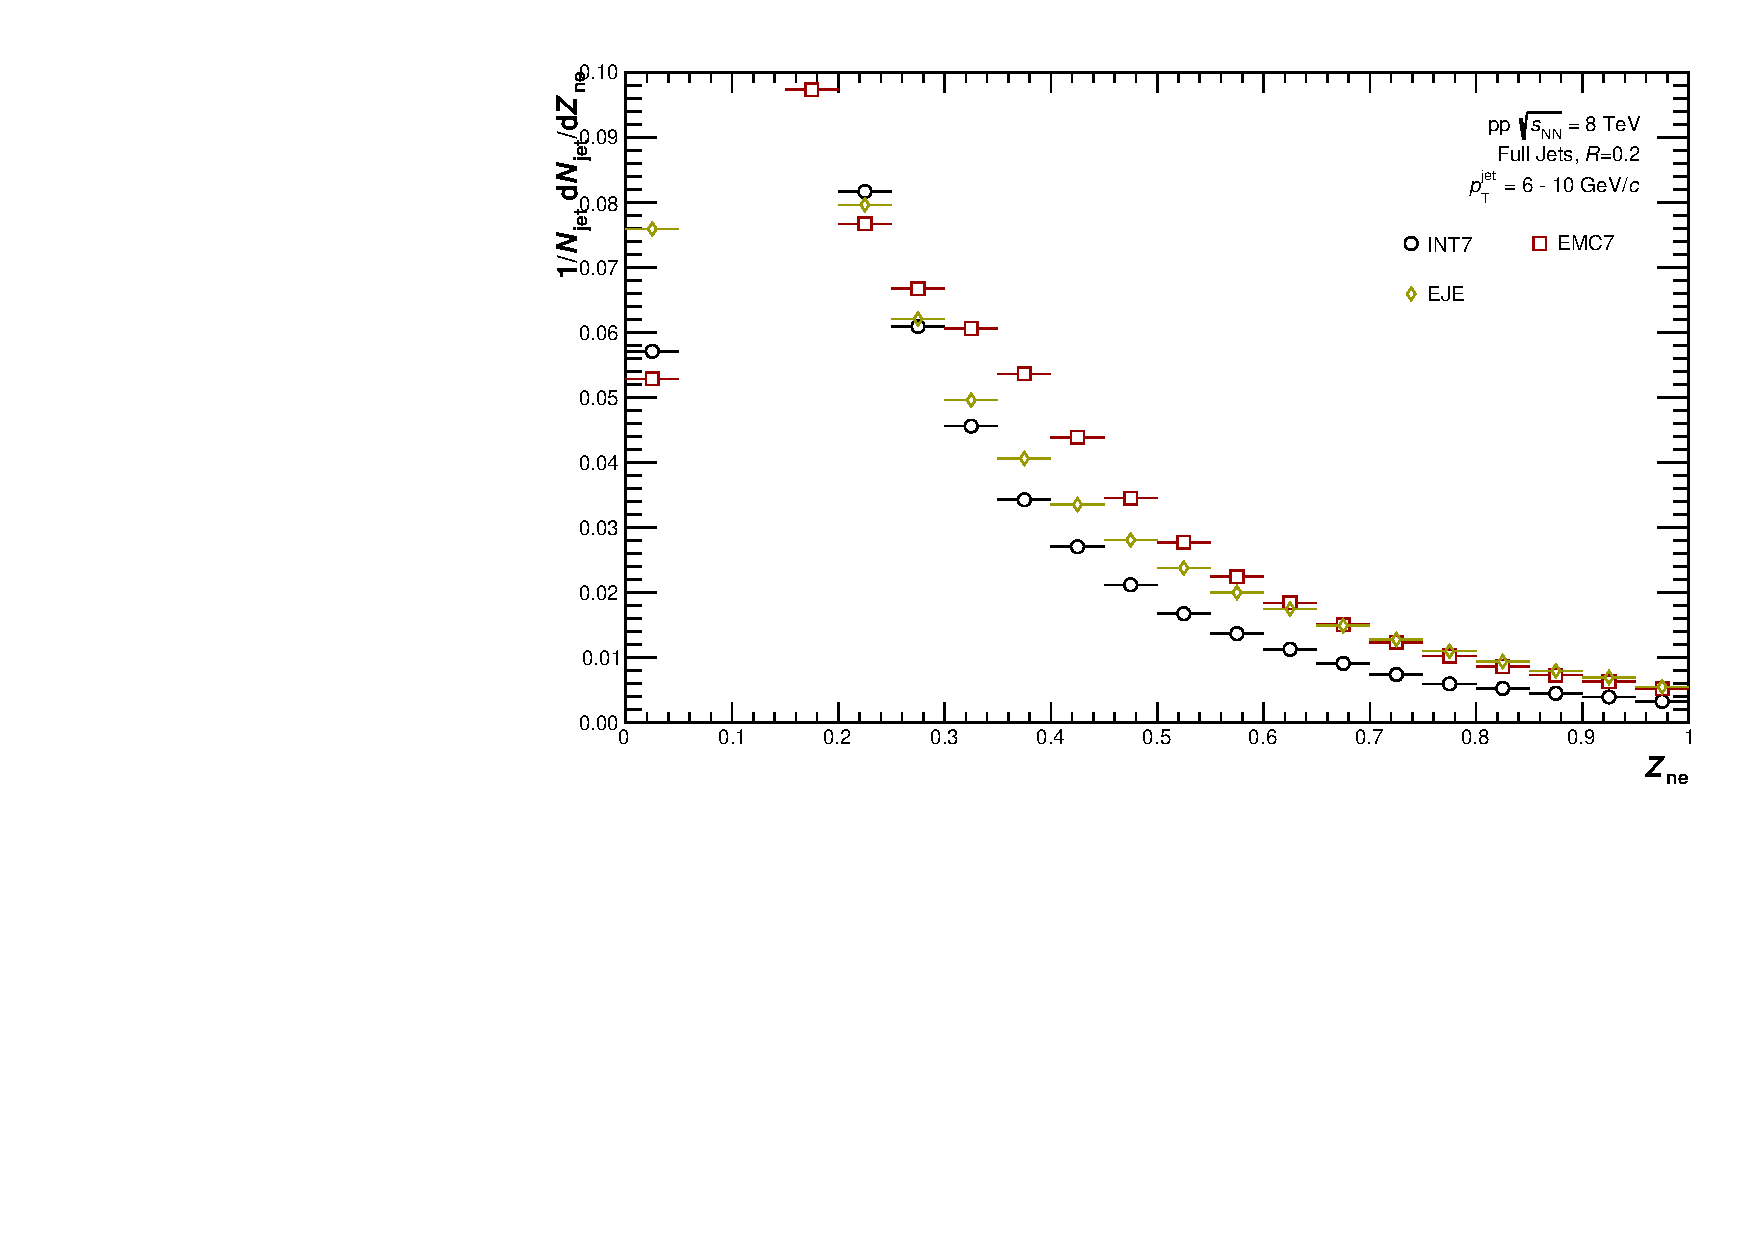
\includegraphics[width=.45\textwidth]{figures/Zne/All/hZne_6-10GeV_R02.pdf}}
    \qquad
    \subfigure{\label{fig:Zne_10-20GeV_R02}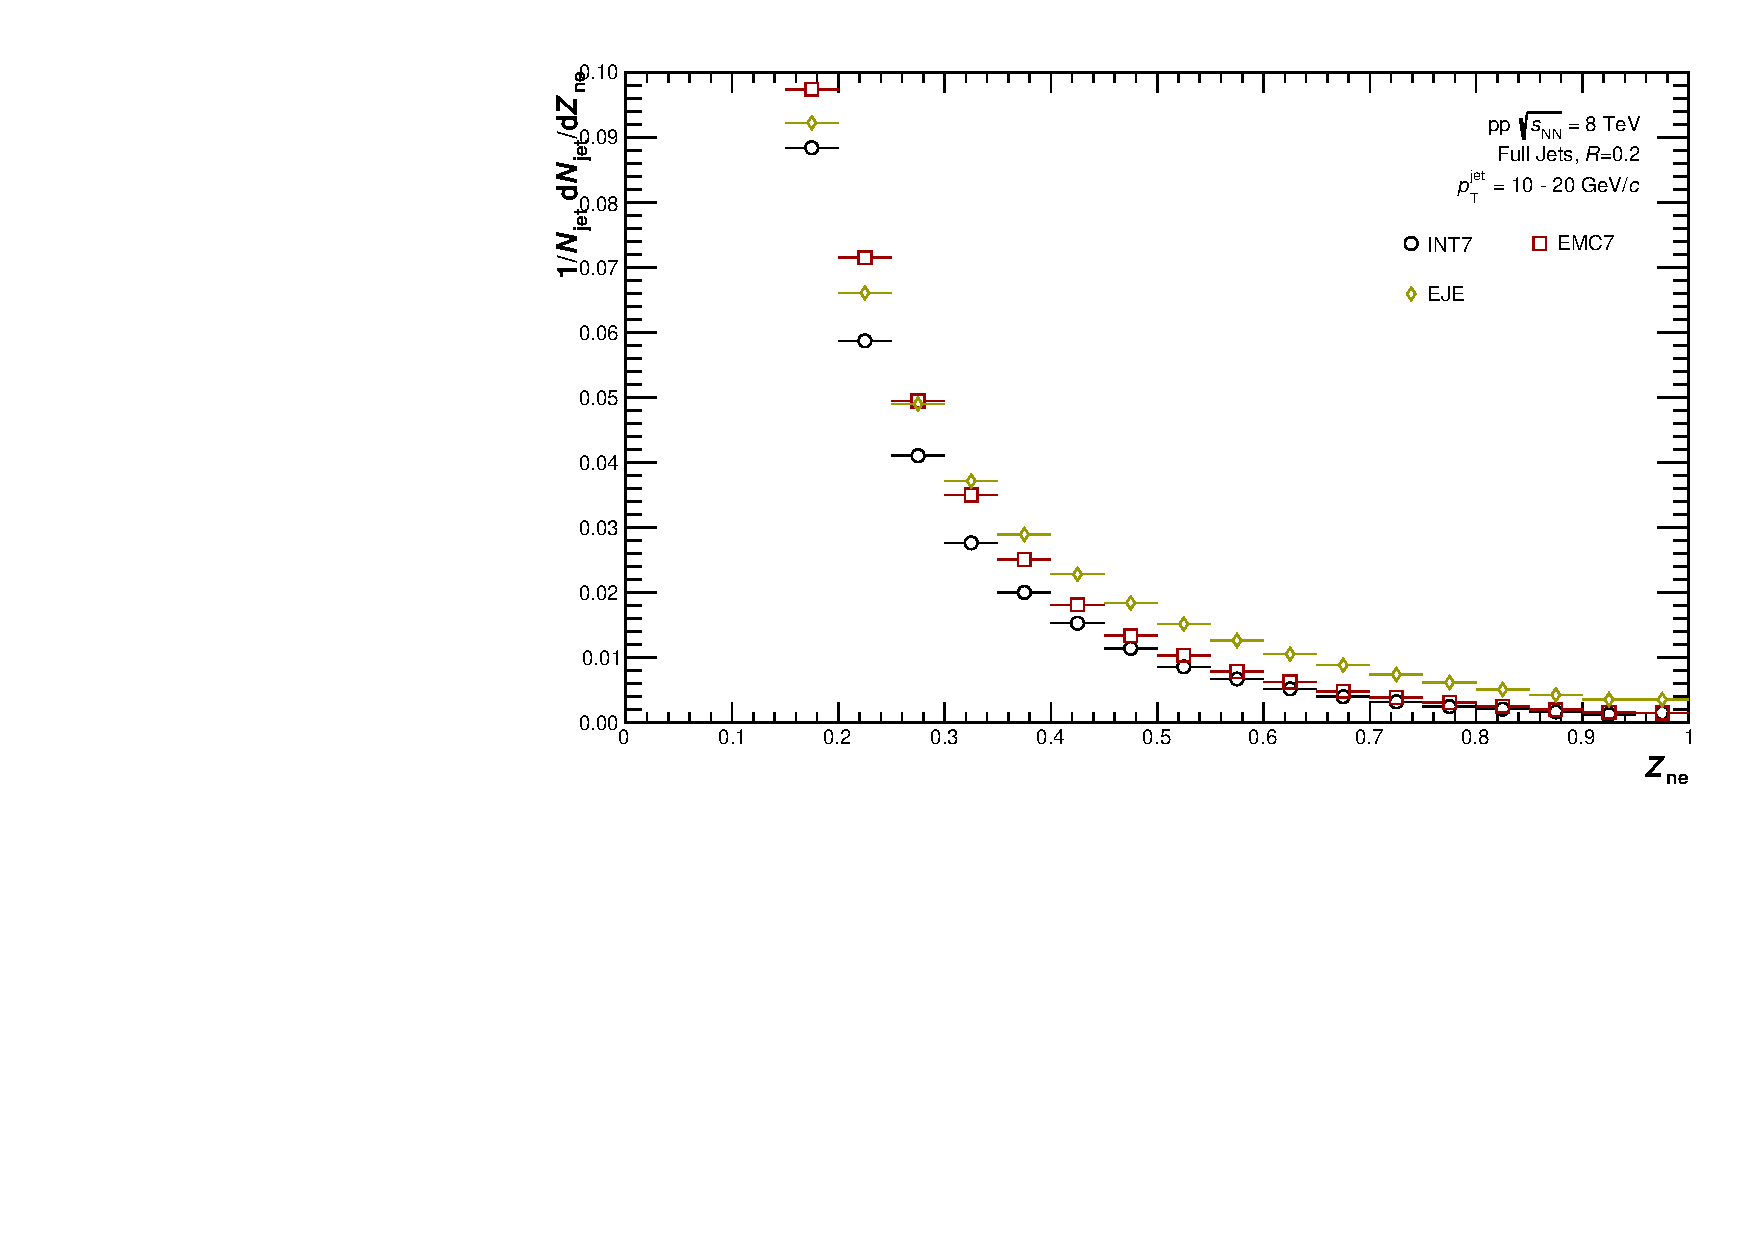
\includegraphics[width=.45\textwidth]{figures/Zne/All/hZne_10-20GeV_R02.pdf}}\\
    \subfigure{\label{fig:Zne_20-30GeV_R02}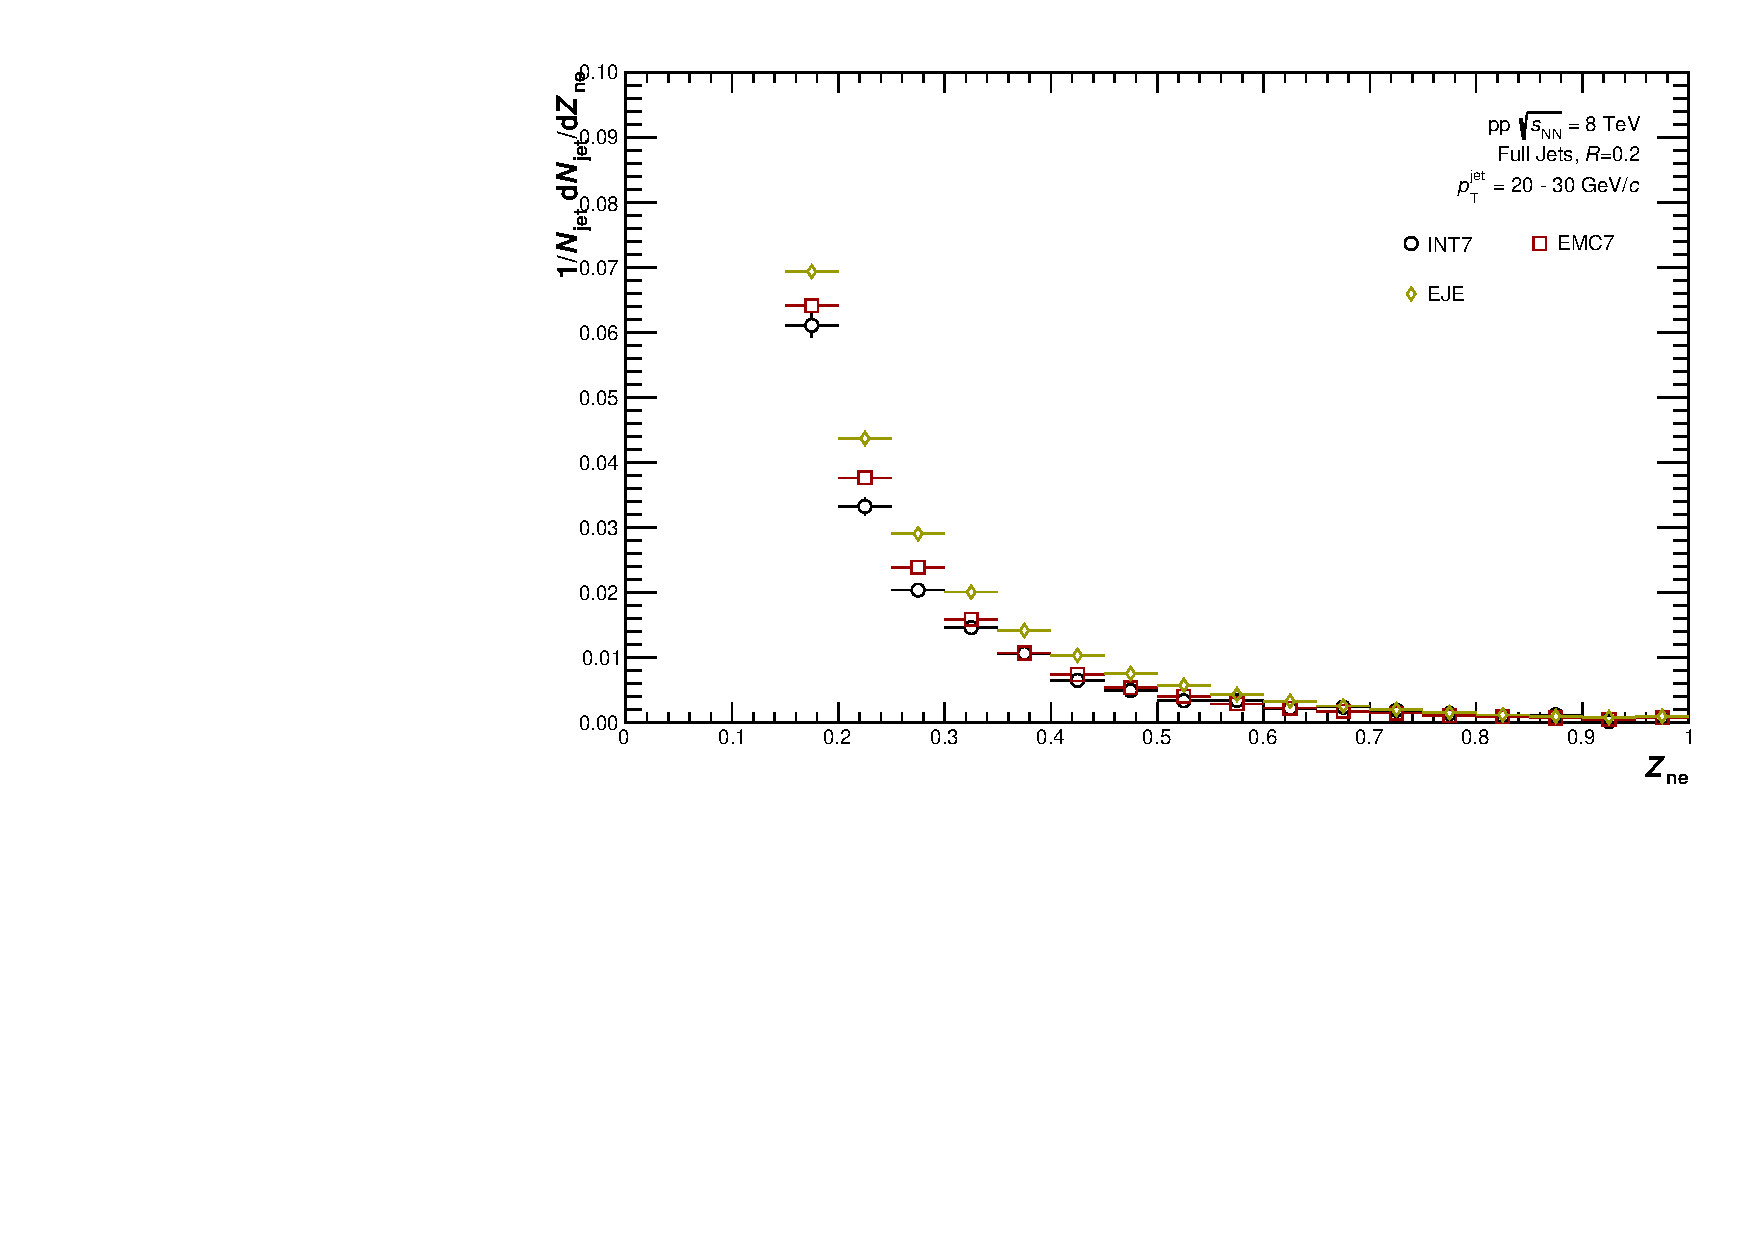
\includegraphics[width=.45\textwidth]{figures/Zne/All/hZne_20-30GeV_R02.pdf}}
    \qquad
    \subfigure{\label{fig:Zne_30-60GeV_R02}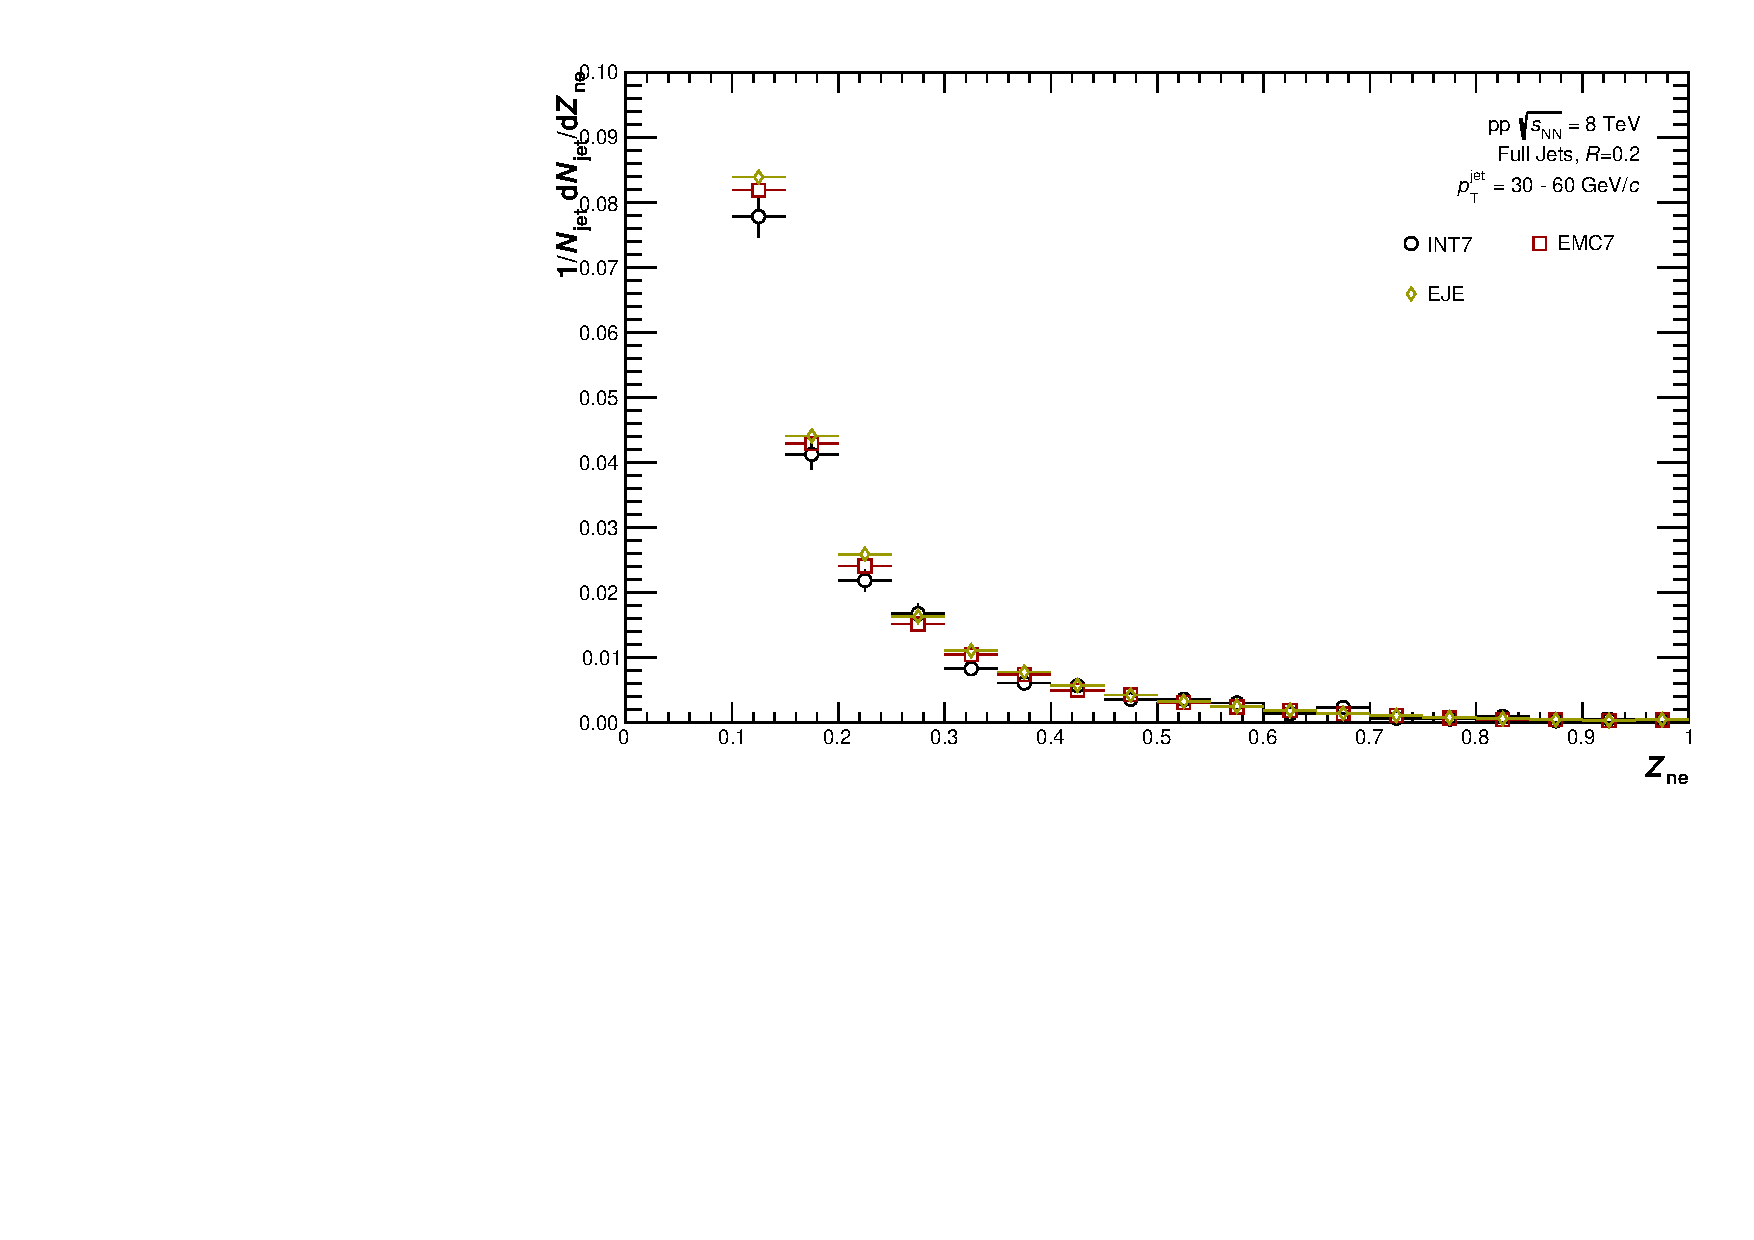
\includegraphics[width=.45\textwidth]{figures/Zne/All/hZne_30-60GeV_R02.pdf}}\\
    \subfigure{\label{fig:Zne_60-100GeV_R02}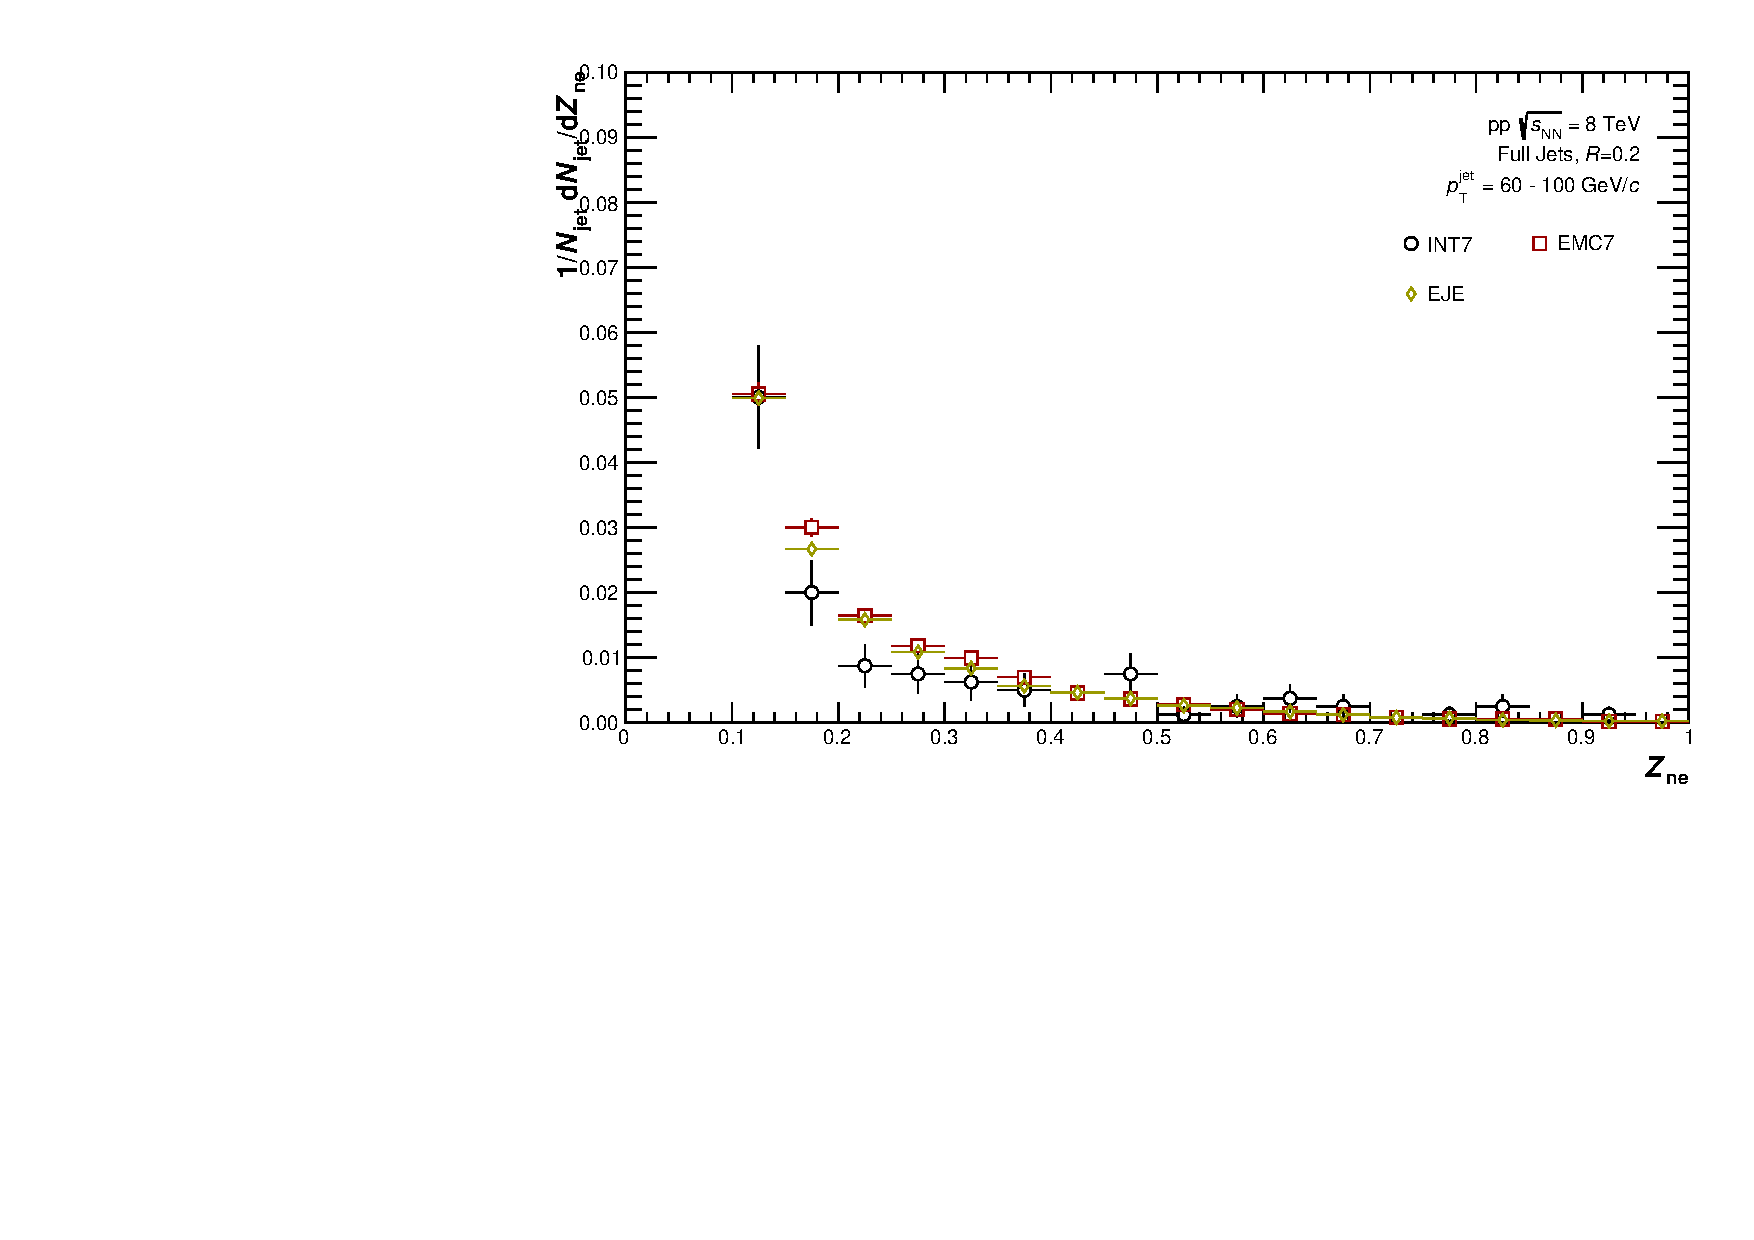
\includegraphics[width=.45\textwidth]{figures/Zne/All/hZne_60-100GeV_R02.pdf}}
    \qquad
    \subfigure{\label{fig:Zne_100-200GeV_R02}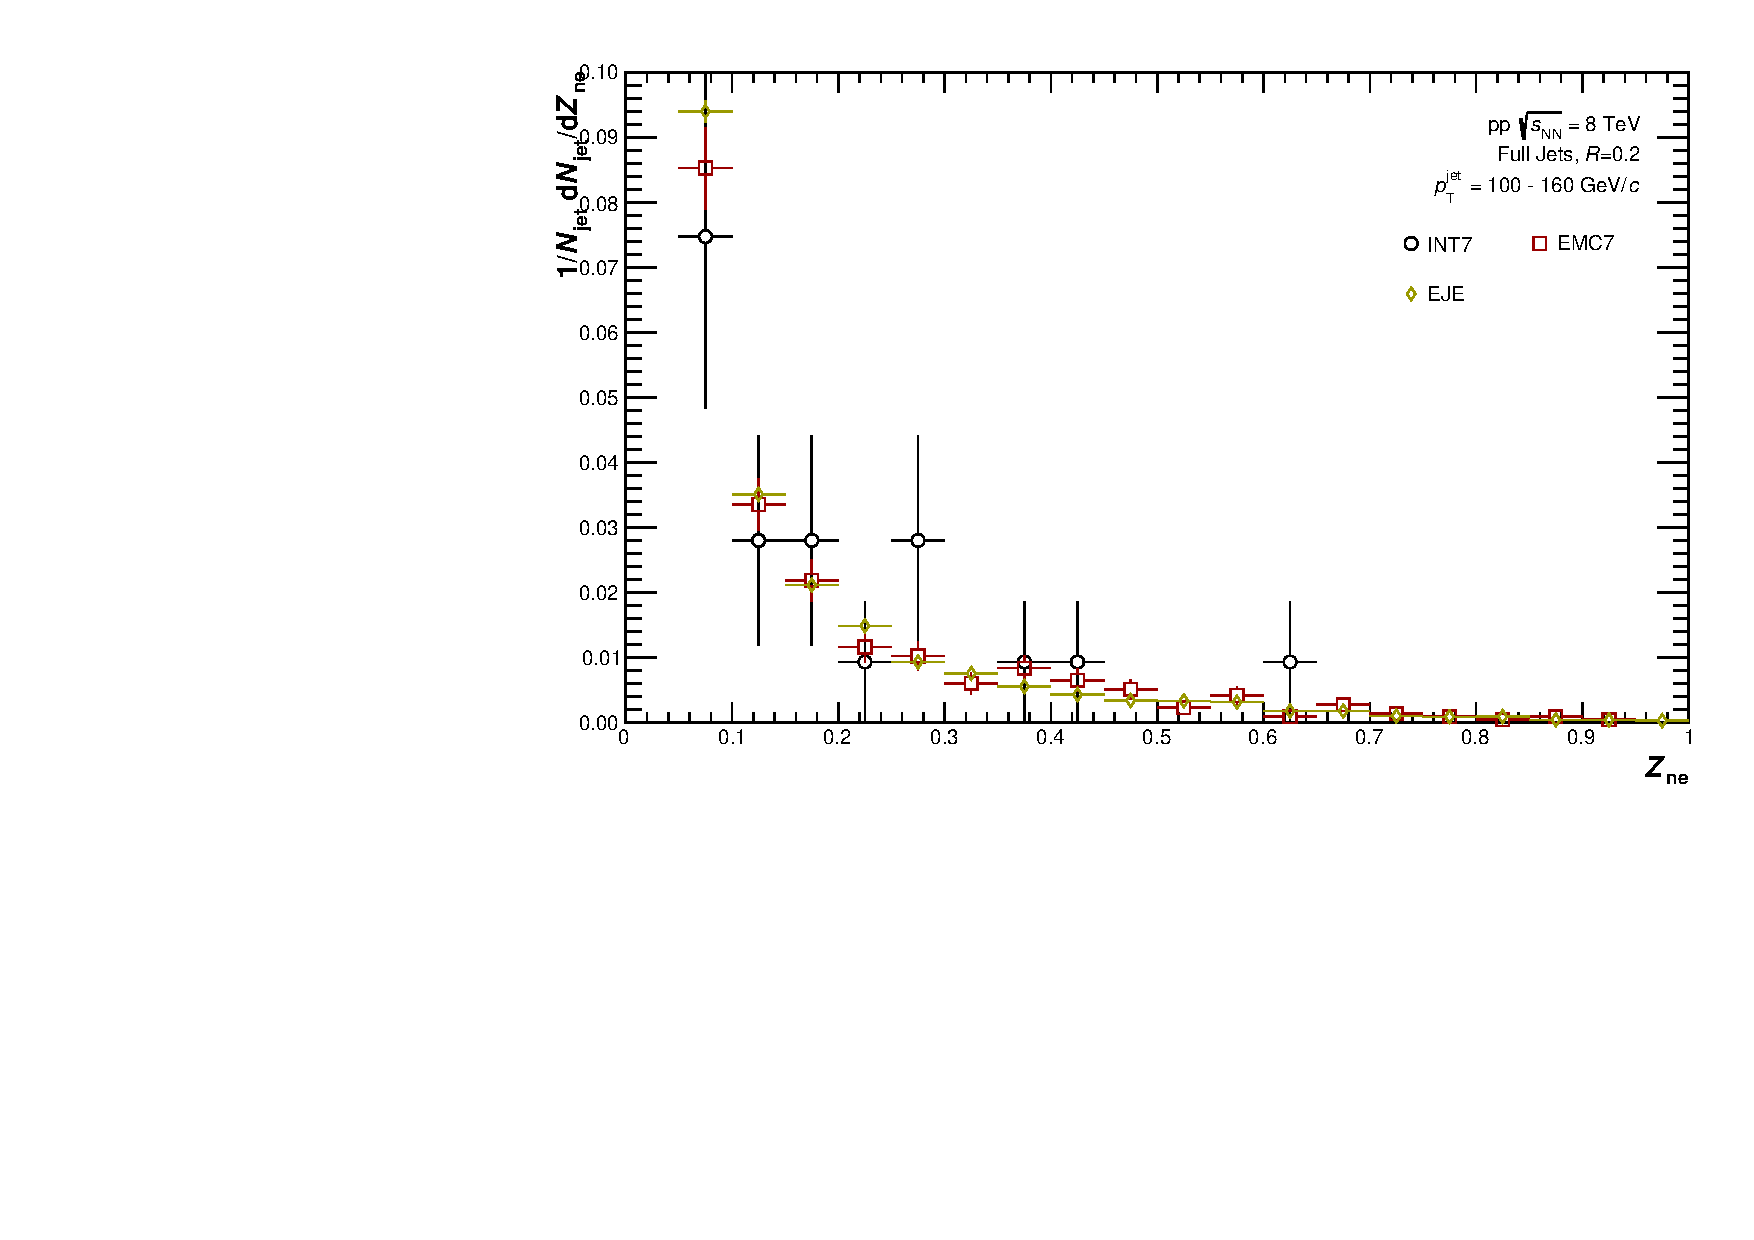
\includegraphics[width=.45\textwidth]{figures/Zne/All/hZne_100-160GeV_R02.pdf}}\\
    \subfigure{\label{fig:Zne_200-350GeV_R02}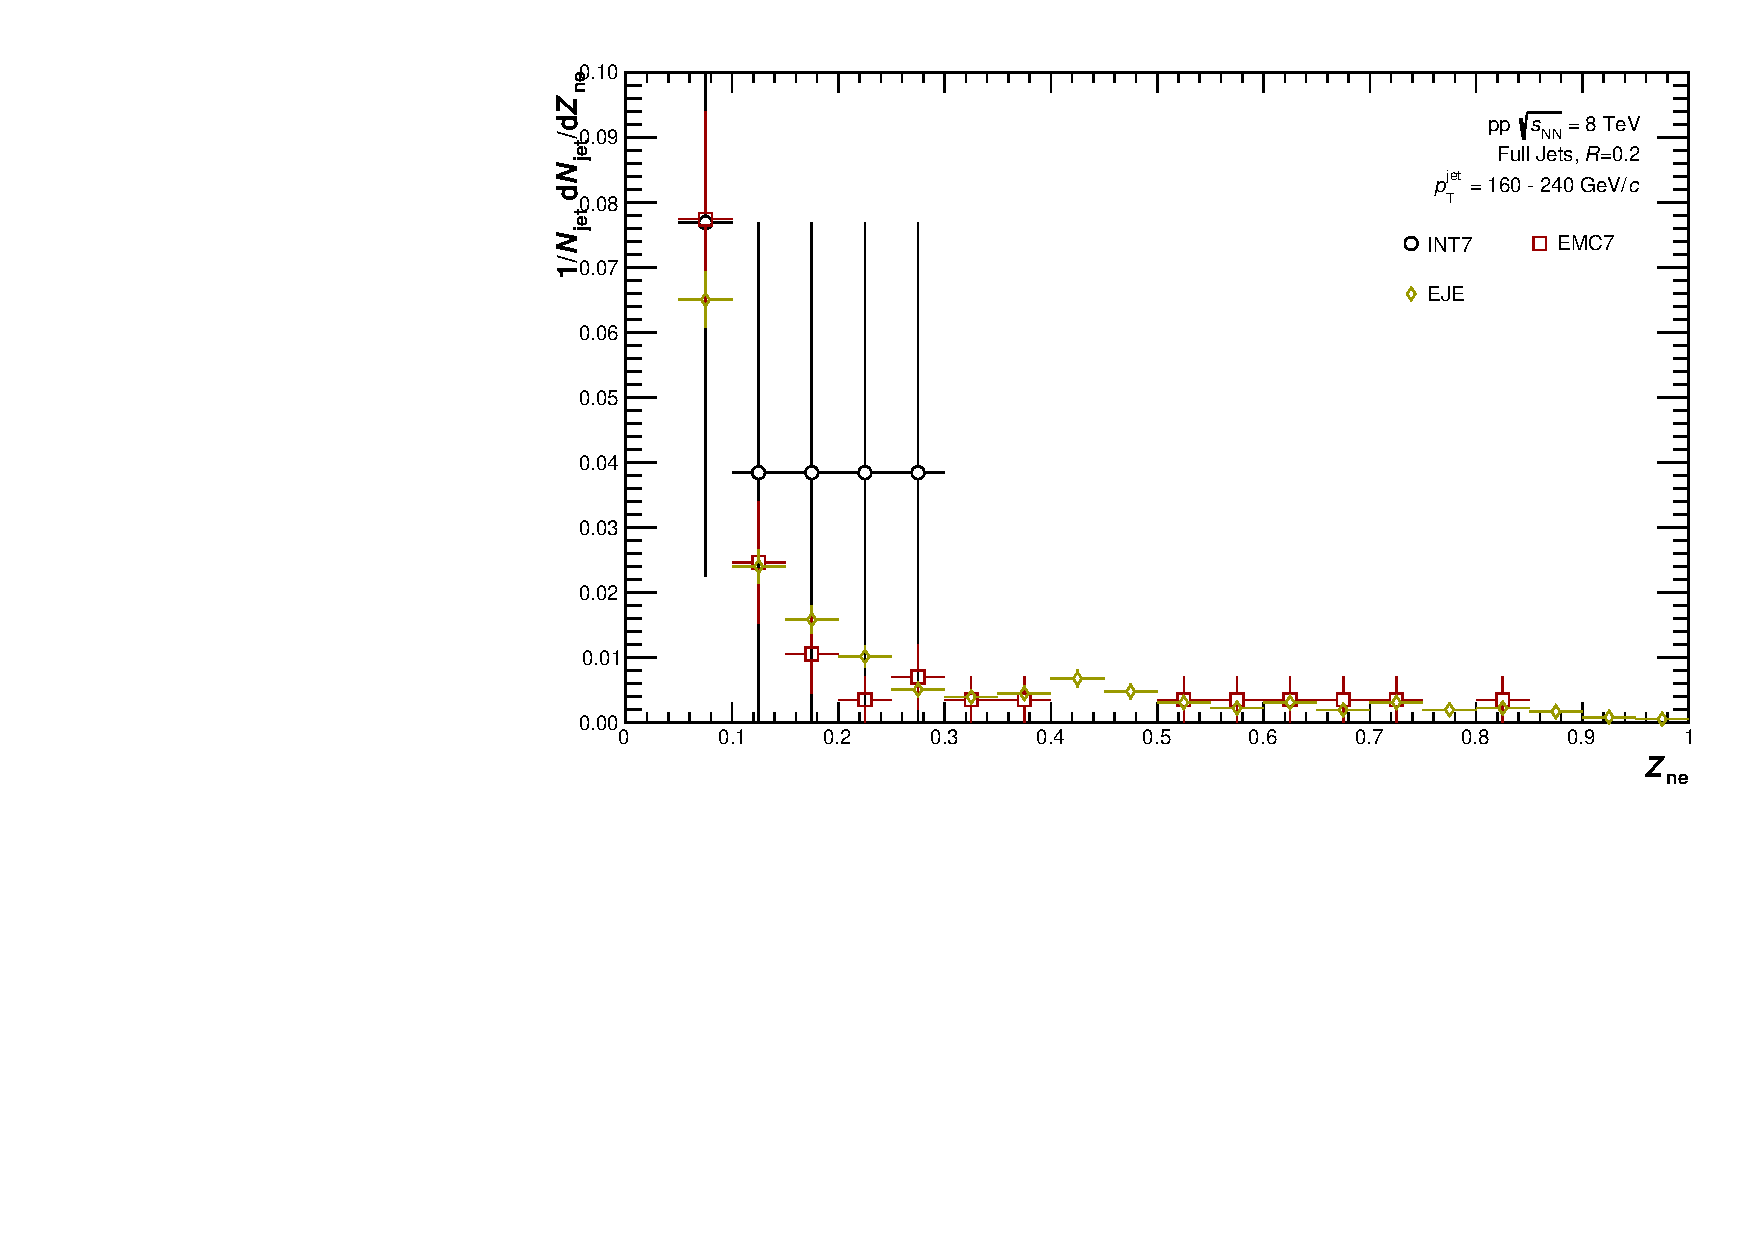
\includegraphics[width=.45\textwidth]{figures/Zne/All/hZne_160-240GeV_R02.pdf}}
    \caption{Z$_{ne}$ for R=0.2 jets in several bins of \pT}
    \label{fig:TriggerBiasZneR02}
\end{figure}

%%%%%%%%%%%%%%%%%%%%%%%%%%%%%%%%%%%%%%%% R=0.3
\newpage

\begin{figure}[h!]
    \centering
    \subfigure{\label{fig:NEF_6-10GeV_R03}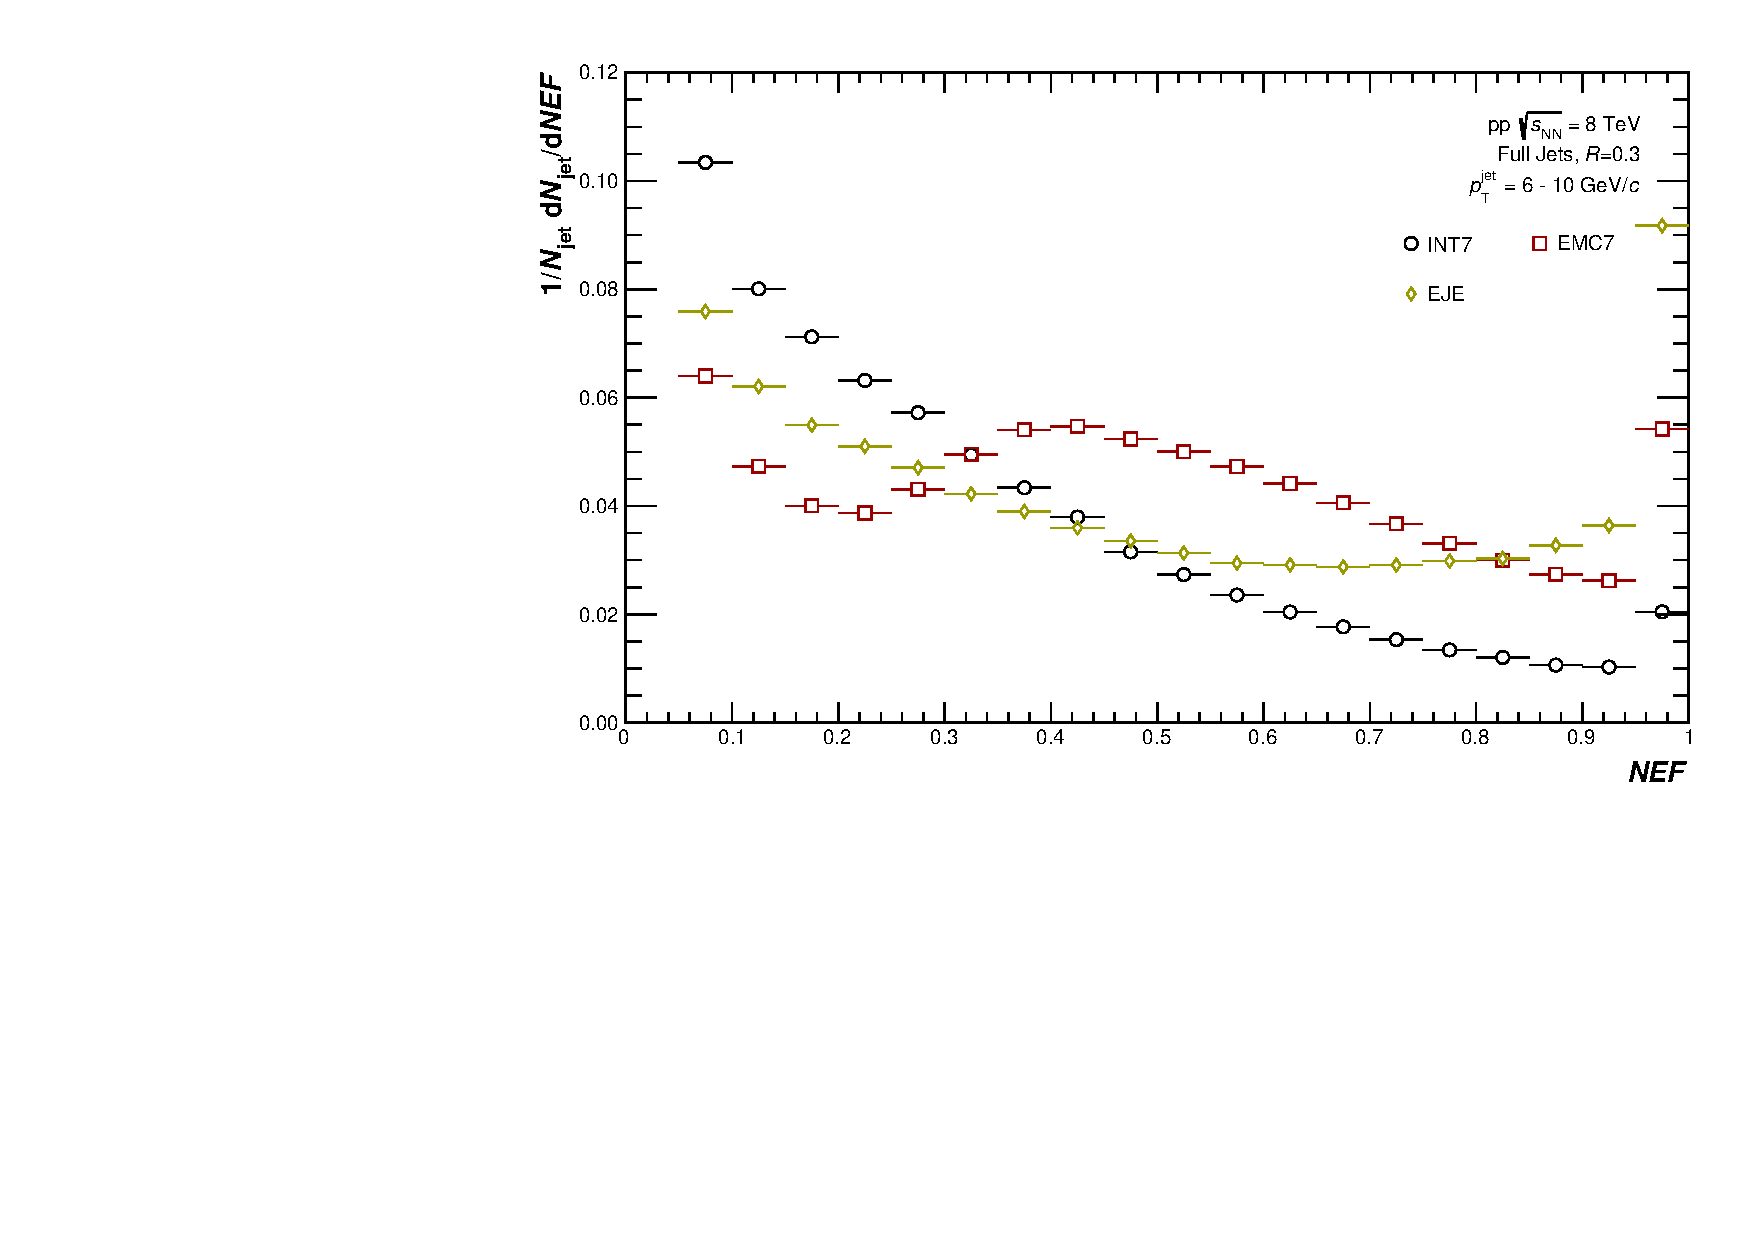
\includegraphics[width=.45\textwidth]{figures/NEF/All/hNEF_6-10GeV_R03.pdf}}
    \qquad
    \subfigure{\label{fig:NEF_10-20GeV_R03}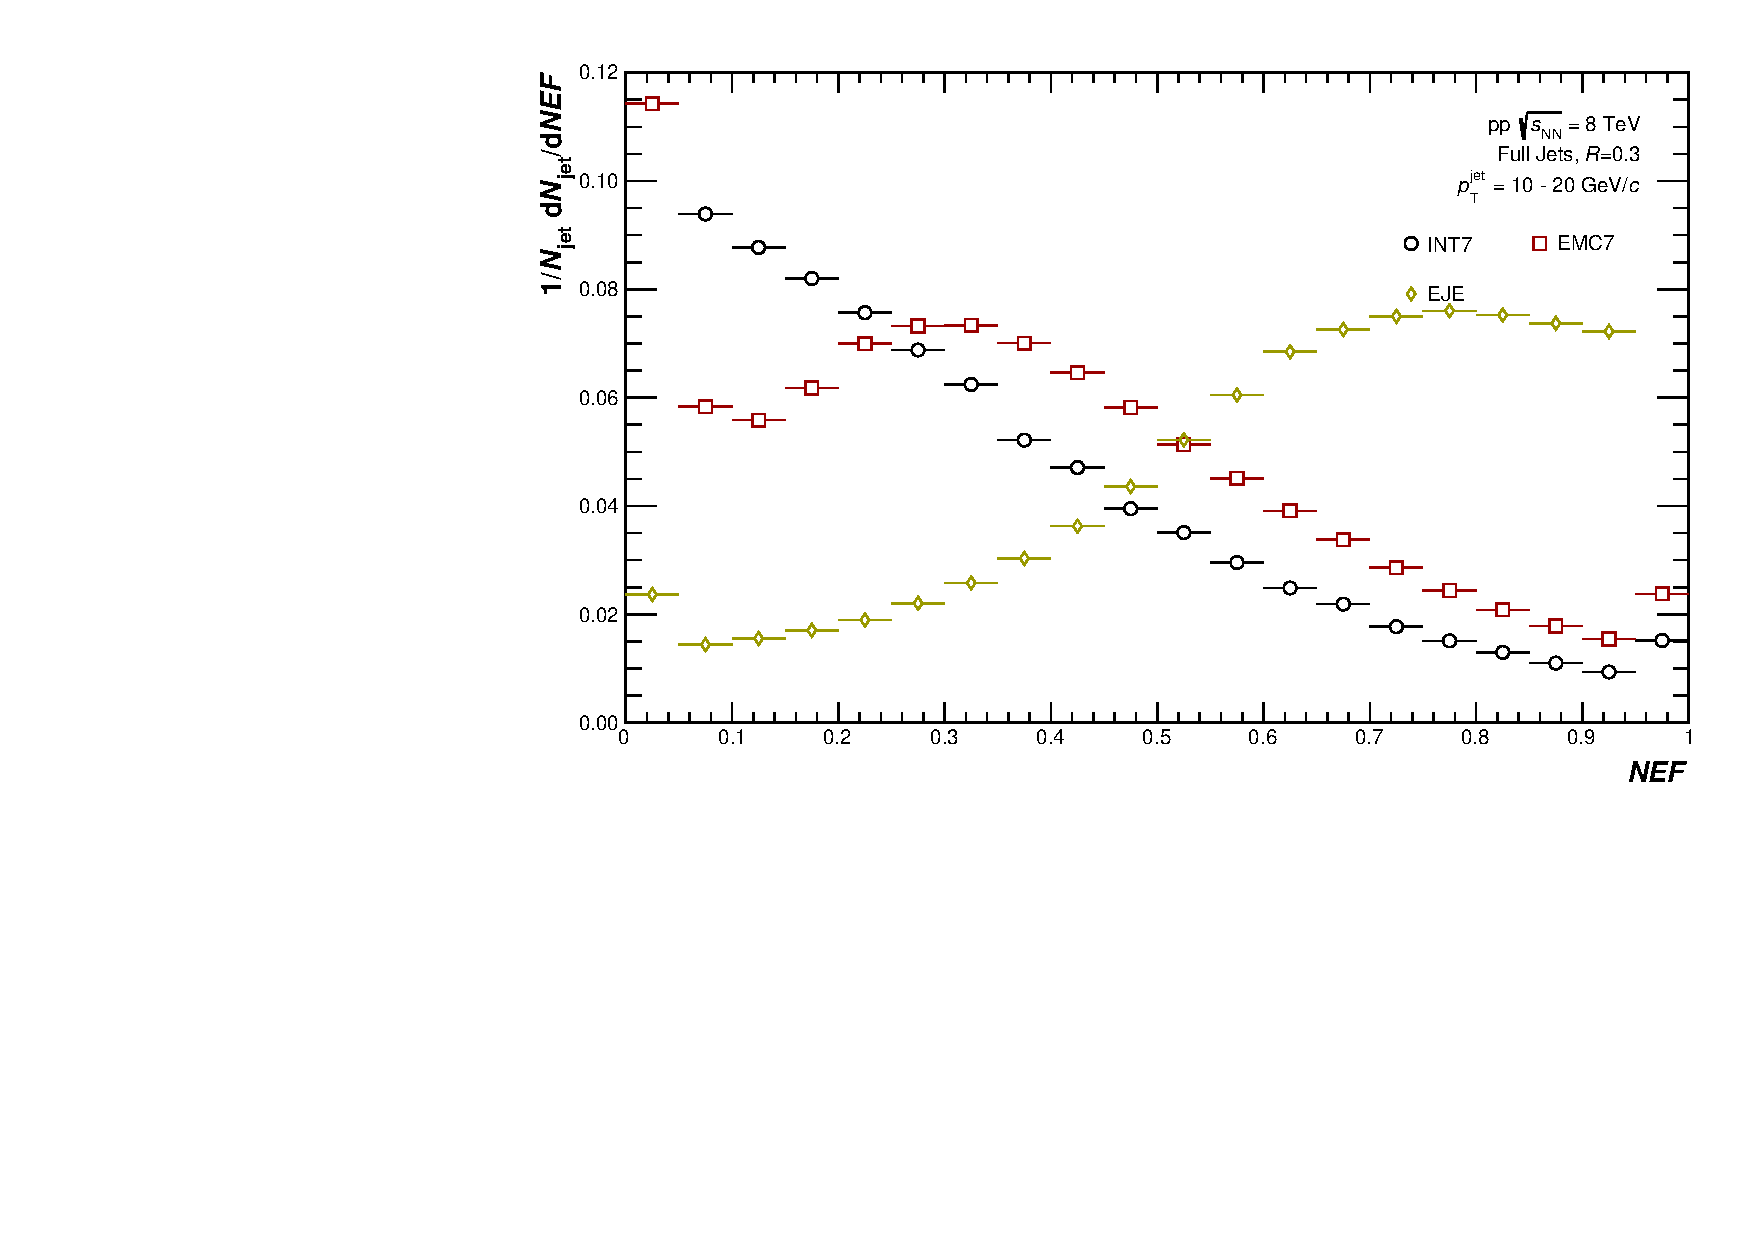
\includegraphics[width=.45\textwidth]{figures/NEF/All/hNEF_10-20GeV_R03.pdf}}\\
    \subfigure{\label{fig:NEF_20-30GeV_R03}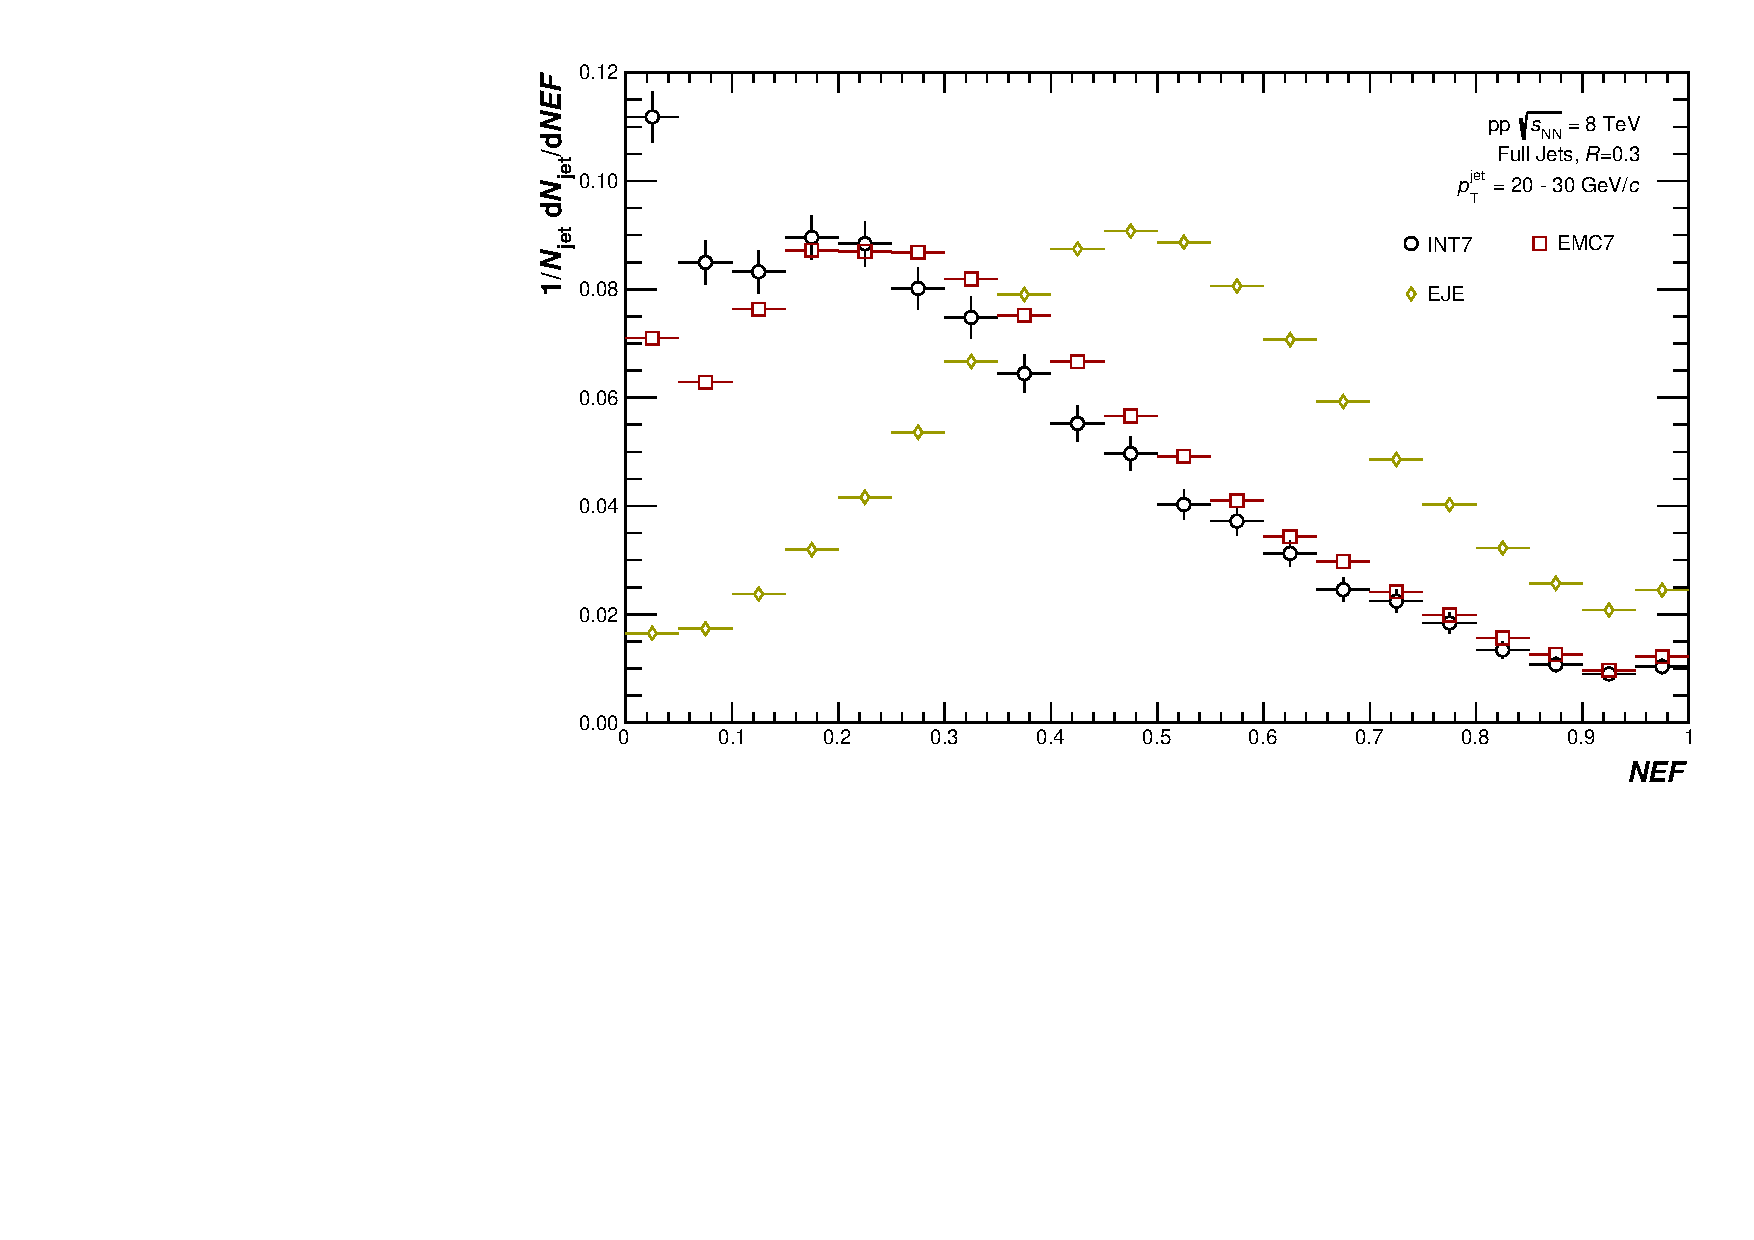
\includegraphics[width=.45\textwidth]{figures/NEF/All/hNEF_20-30GeV_R03.pdf}}
    \qquad
    \subfigure{\label{fig:NEF_30-60GeV_R03}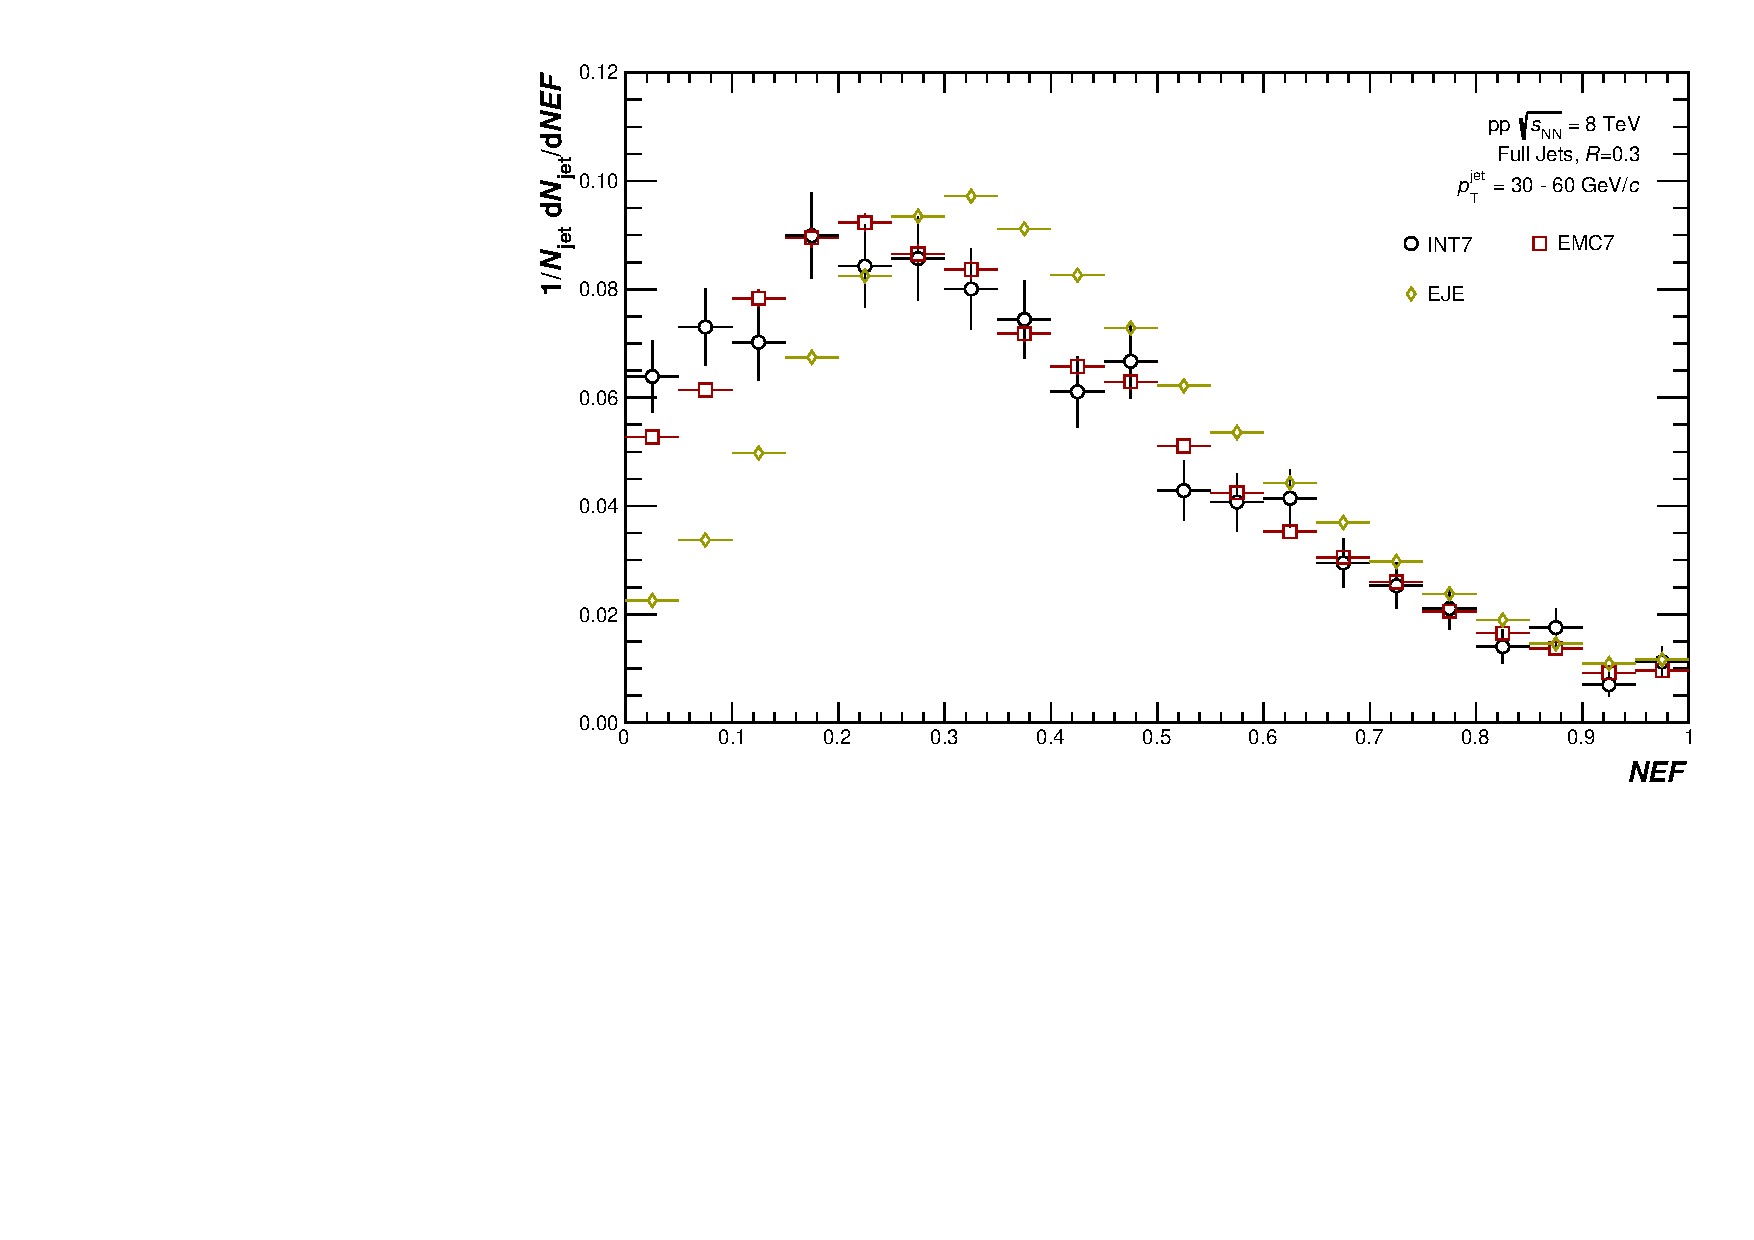
\includegraphics[width=.45\textwidth]{figures/NEF/All/hNEF_30-60GeV_R03.pdf}}\\
    \subfigure{\label{fig:NEF_60-100GeV_R03}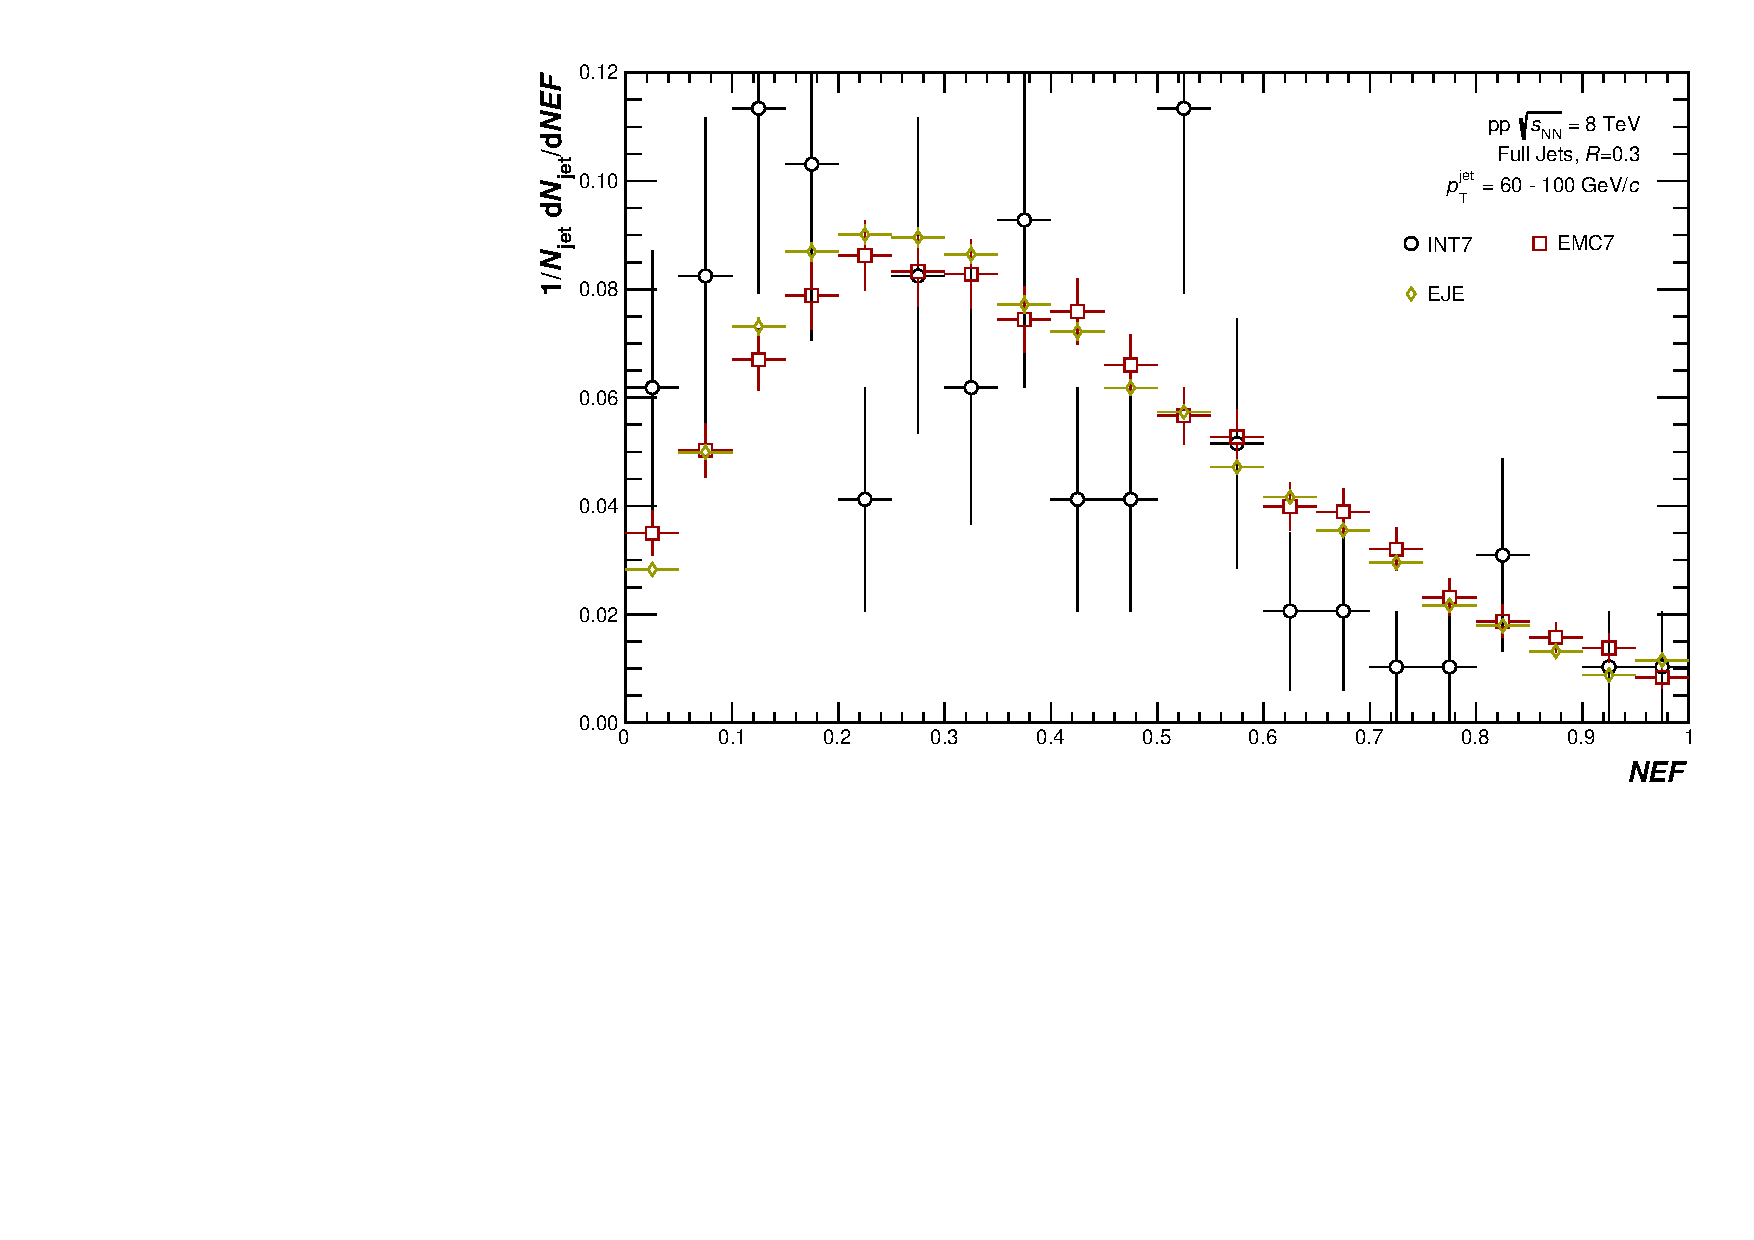
\includegraphics[width=.45\textwidth]{figures/NEF/All/hNEF_60-100GeV_R03.pdf}}
    \qquad
    \subfigure{\label{fig:NEF_100-200GeV_R03}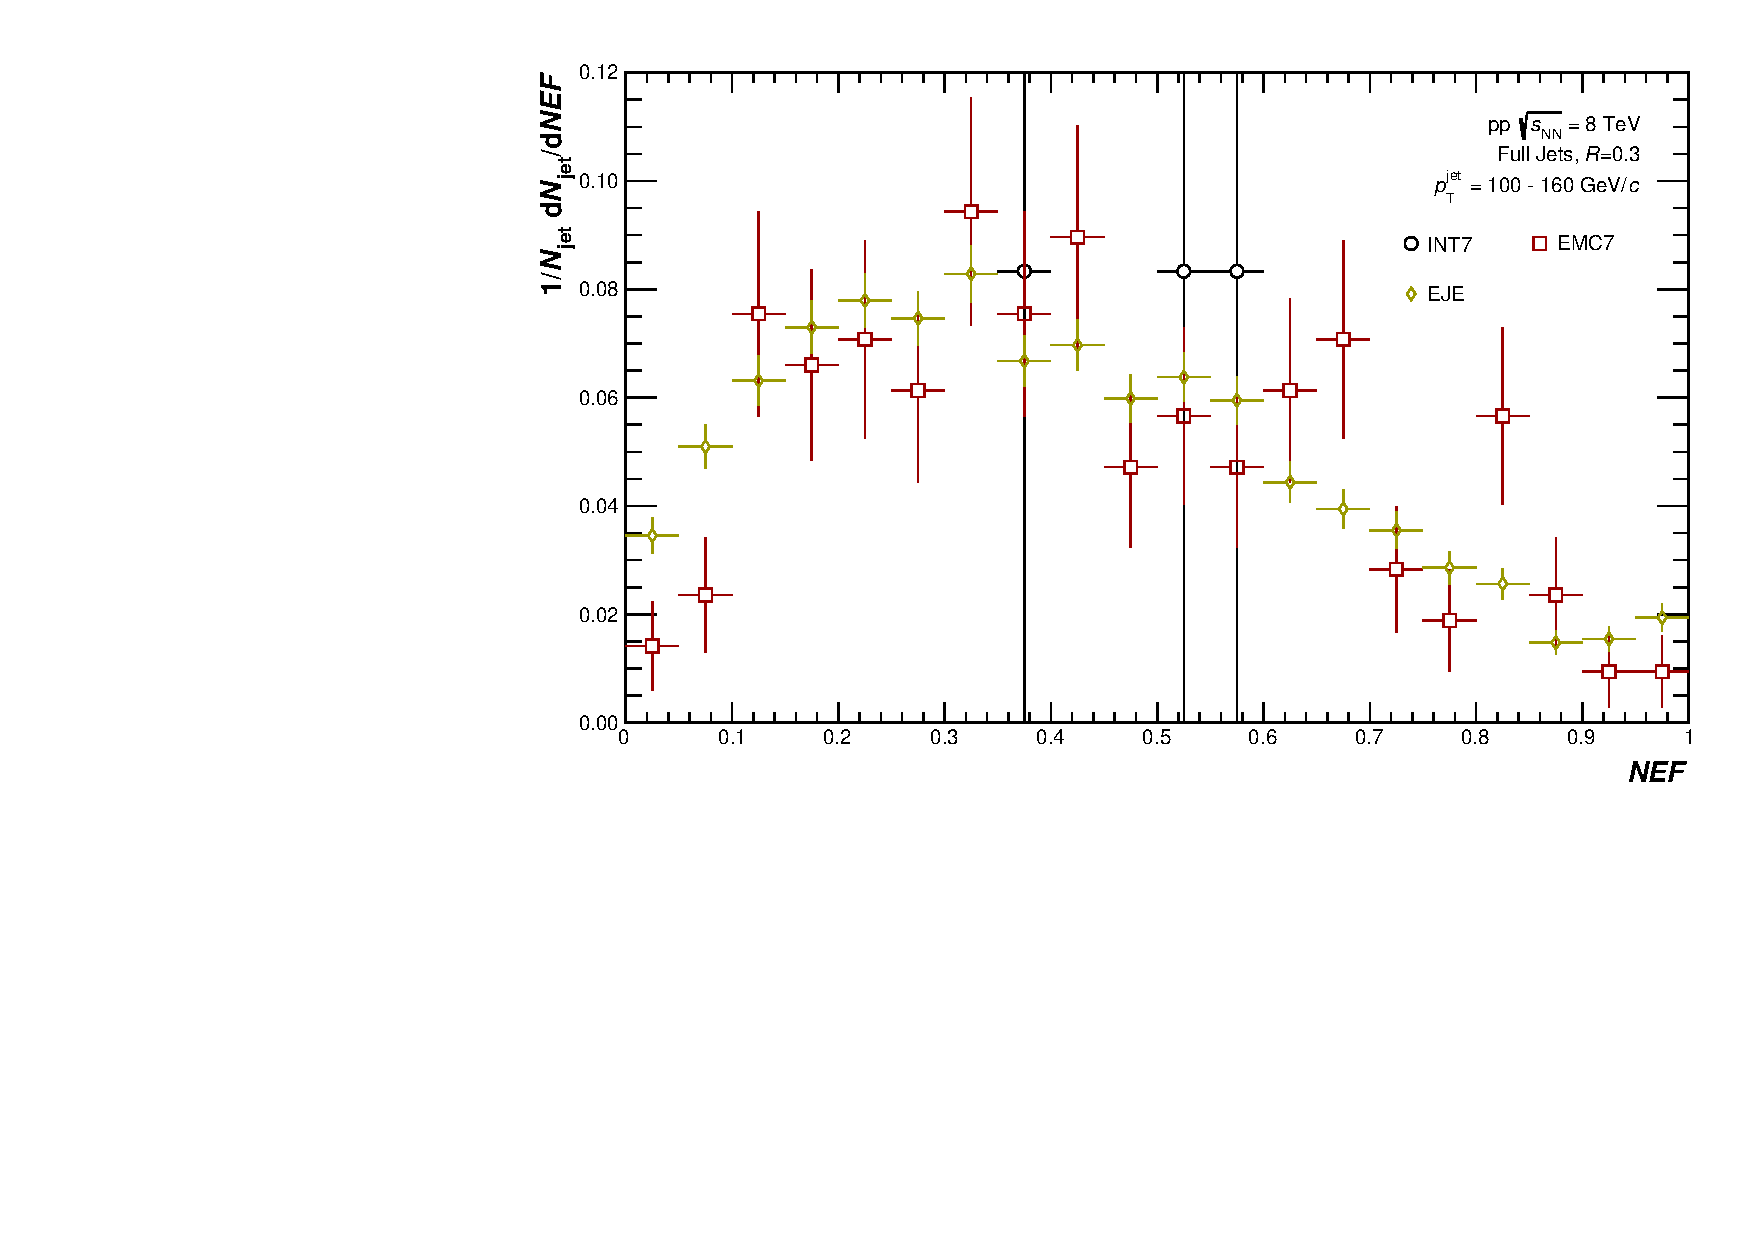
\includegraphics[width=.45\textwidth]{figures/NEF/All/hNEF_100-160GeV_R03.pdf}}\\
    \subfigure{\label{fig:NEF_200-350GeV_R03}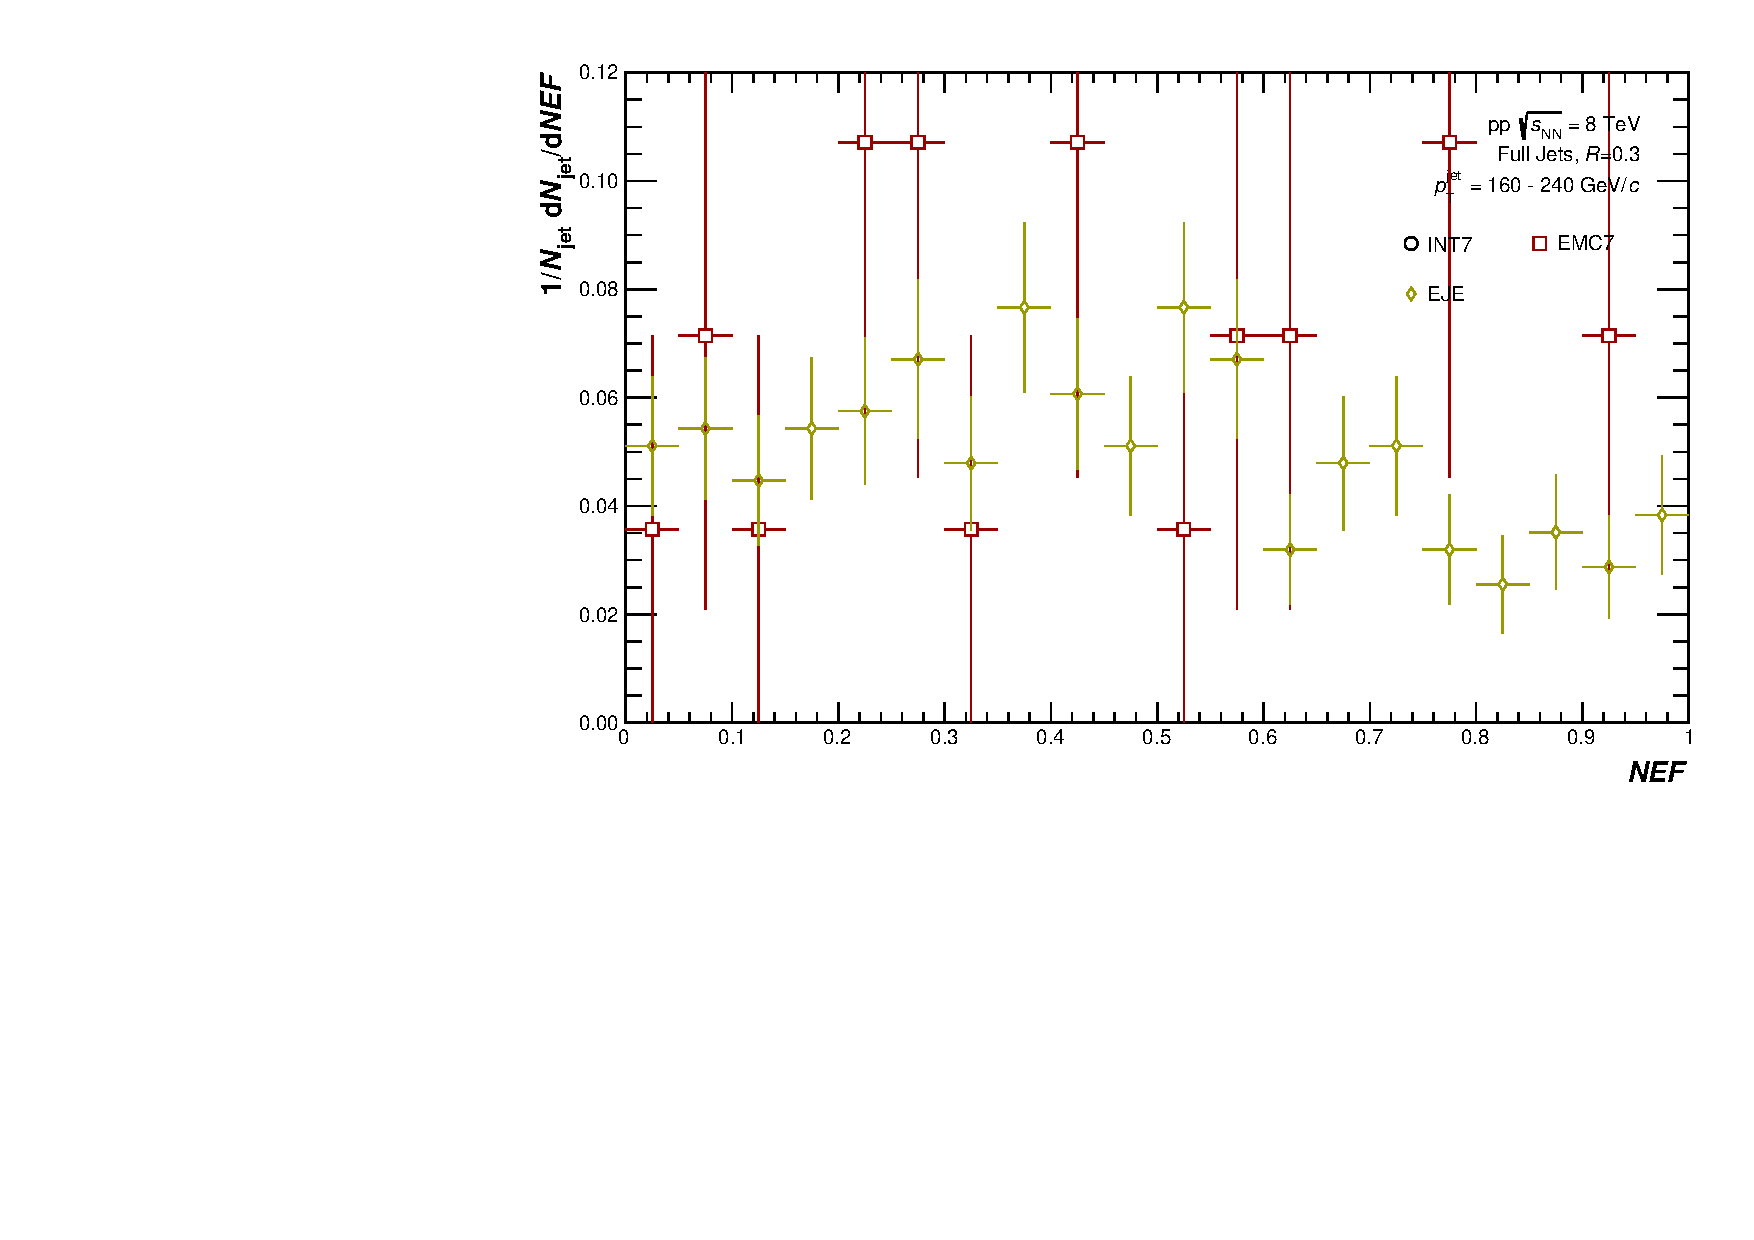
\includegraphics[width=.45\textwidth]{figures/NEF/All/hNEF_160-240GeV_R03.pdf}}
    \caption{NEF for R=0.3 jets in several bins of \pT}
    \label{fig:TriggerBiasNEFR03}
\end{figure}

\newpage

\begin{figure}[h!]
    \centering
    \subfigure{\label{fig:Zch_6-10GeV_R03}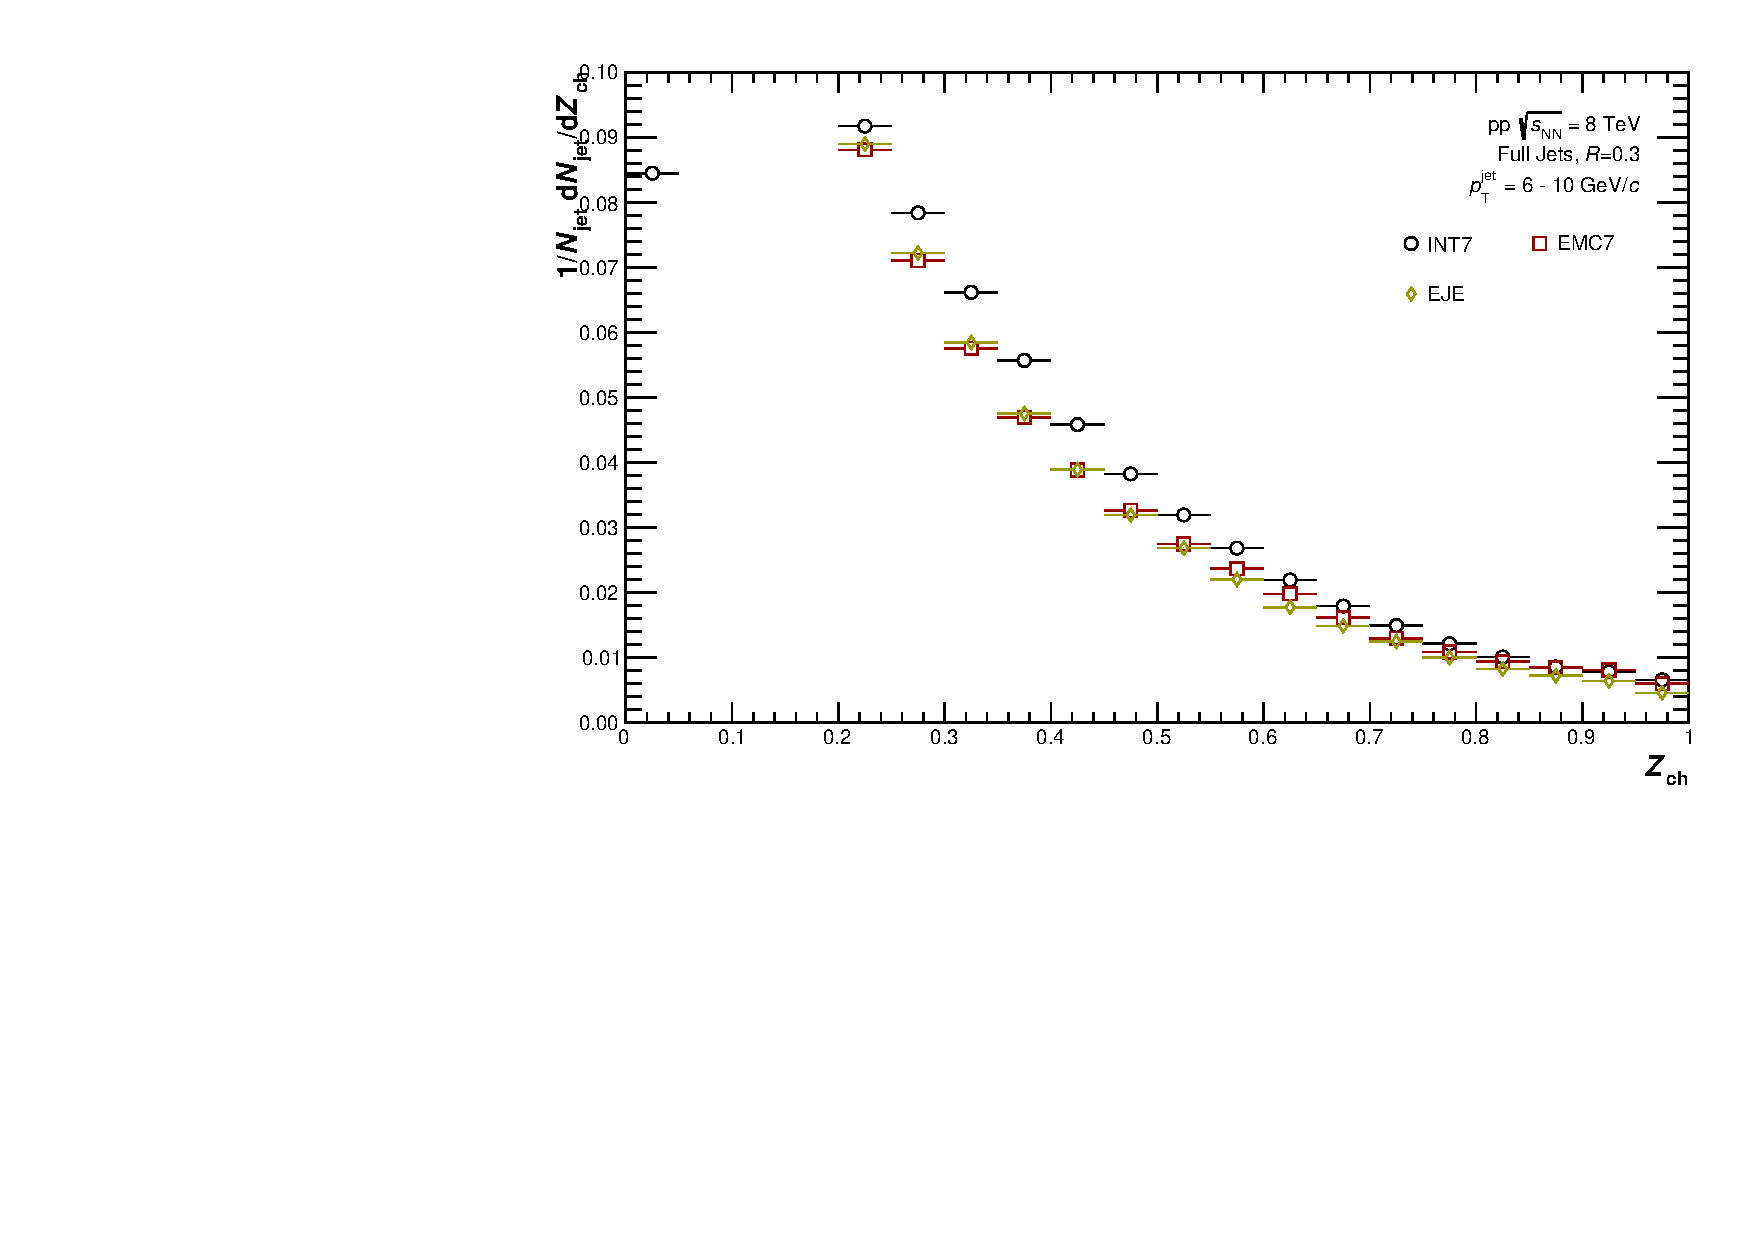
\includegraphics[width=.45\textwidth]{figures/Zch/All/hZch_6-10GeV_R03.pdf}}
    \qquad
    \subfigure{\label{fig:Zch_10-20GeV_R03}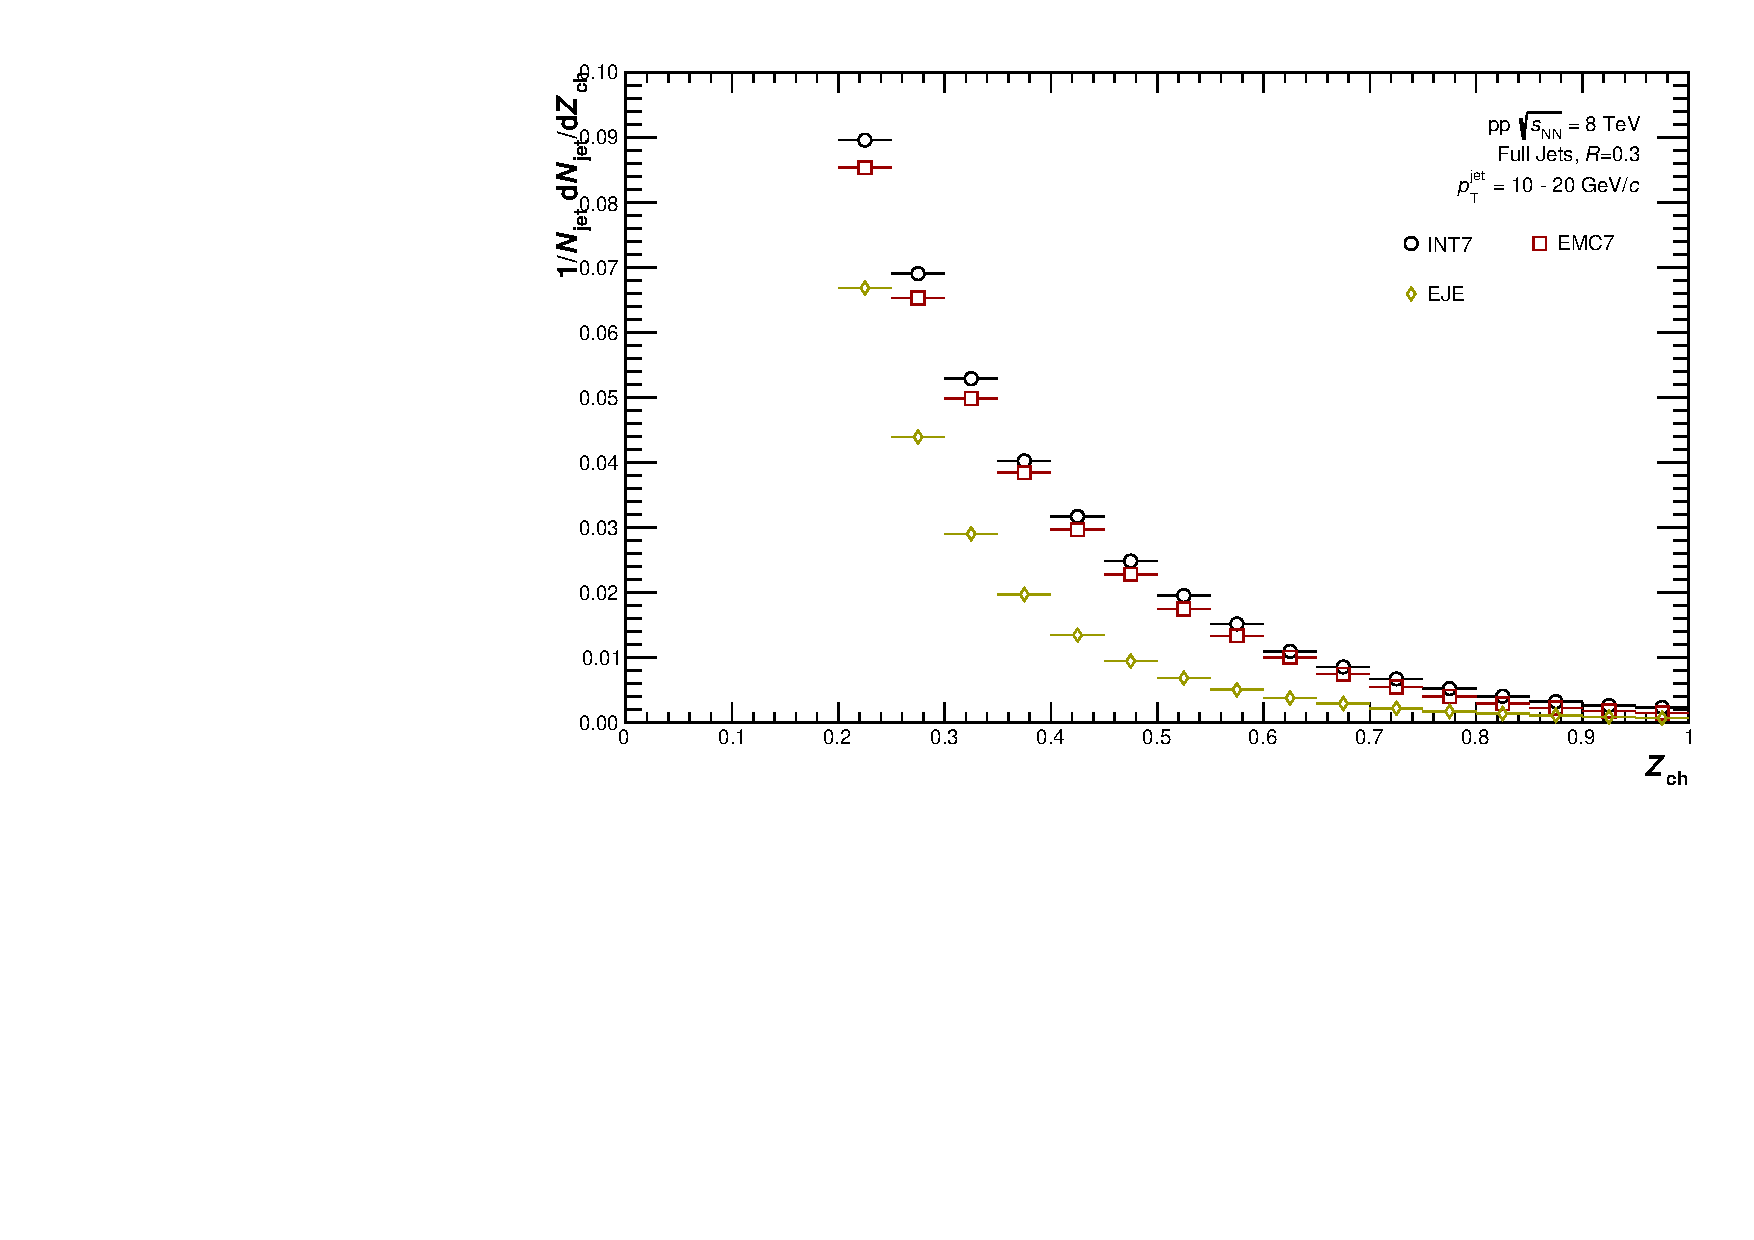
\includegraphics[width=.45\textwidth]{figures/Zch/All/hZch_10-20GeV_R03.pdf}}\\
    \subfigure{\label{fig:Zch_20-30GeV_R03}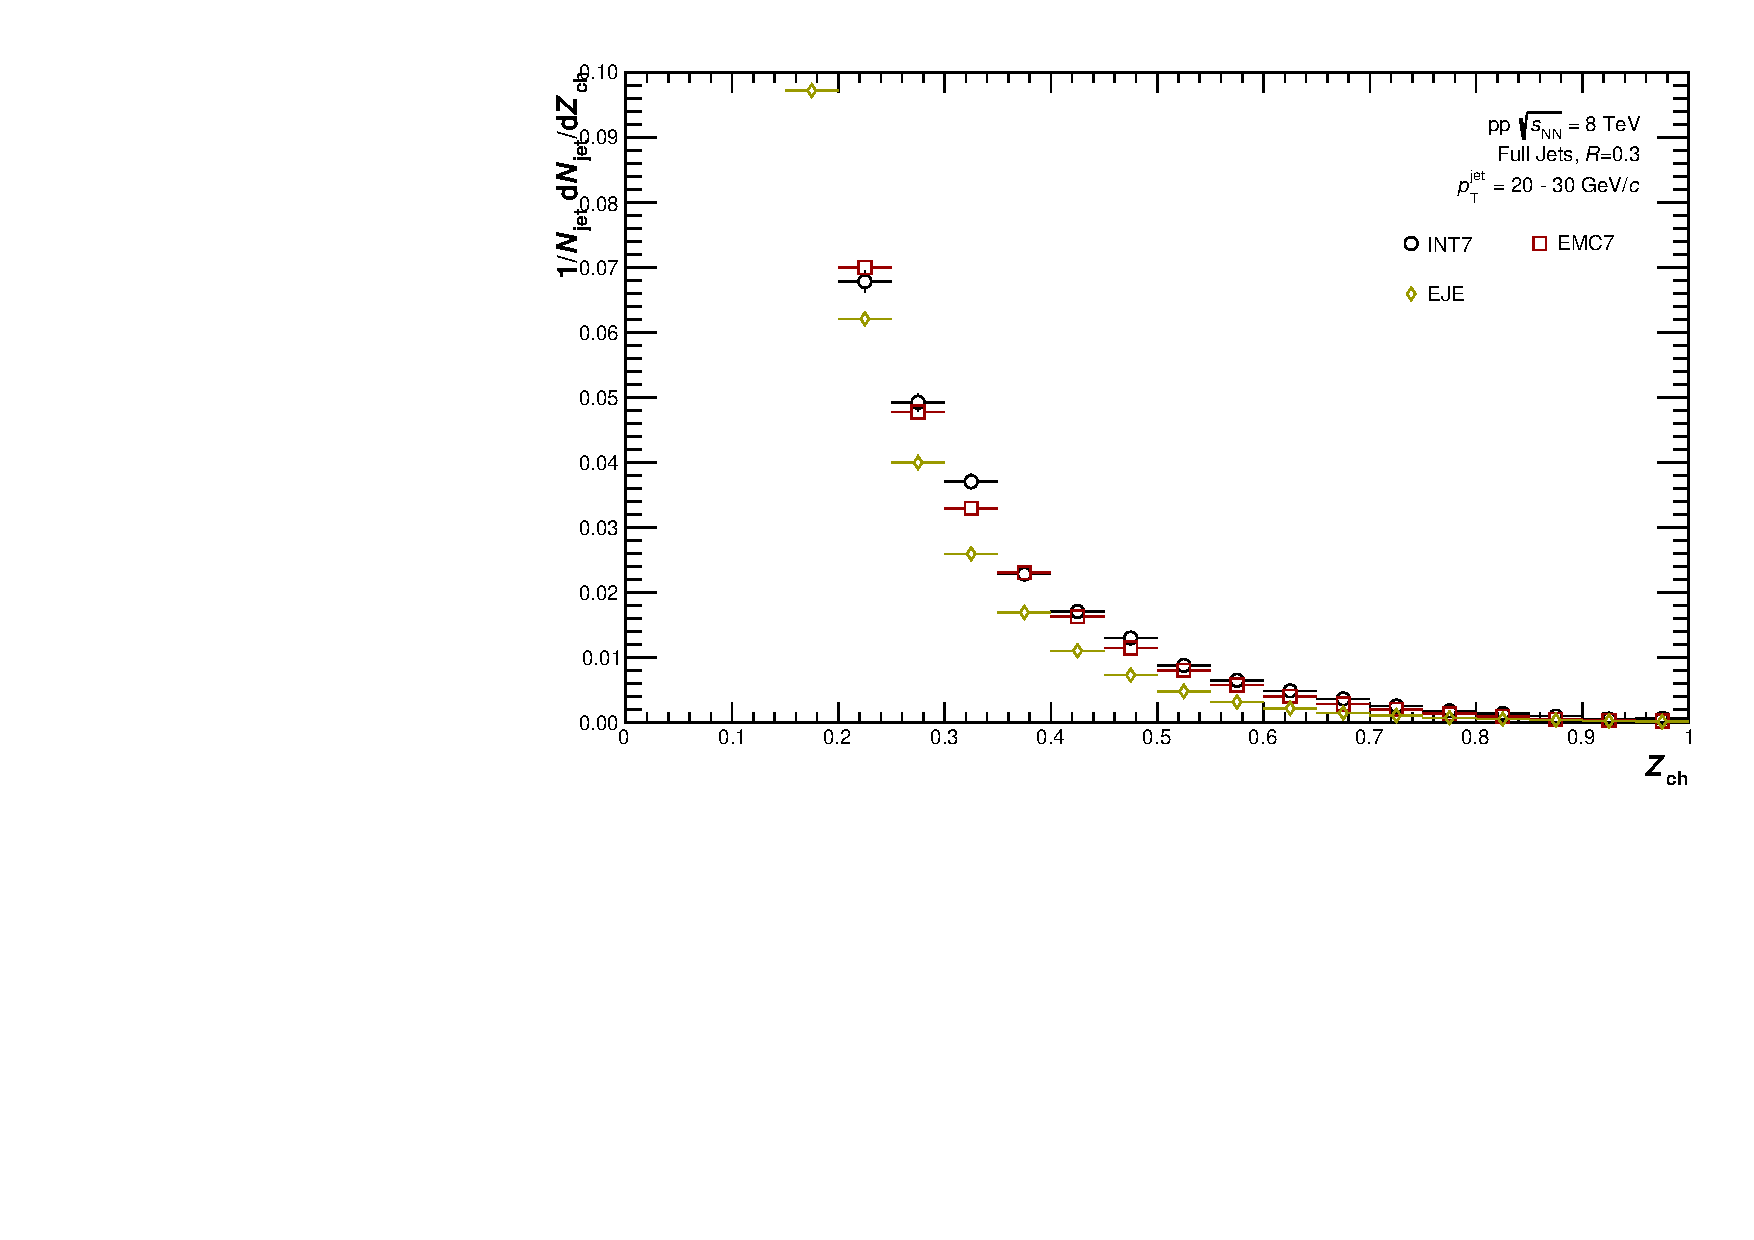
\includegraphics[width=.45\textwidth]{figures/Zch/All/hZch_20-30GeV_R03.pdf}}
    \qquad
    \subfigure{\label{fig:Zch_30-60GeV_R03}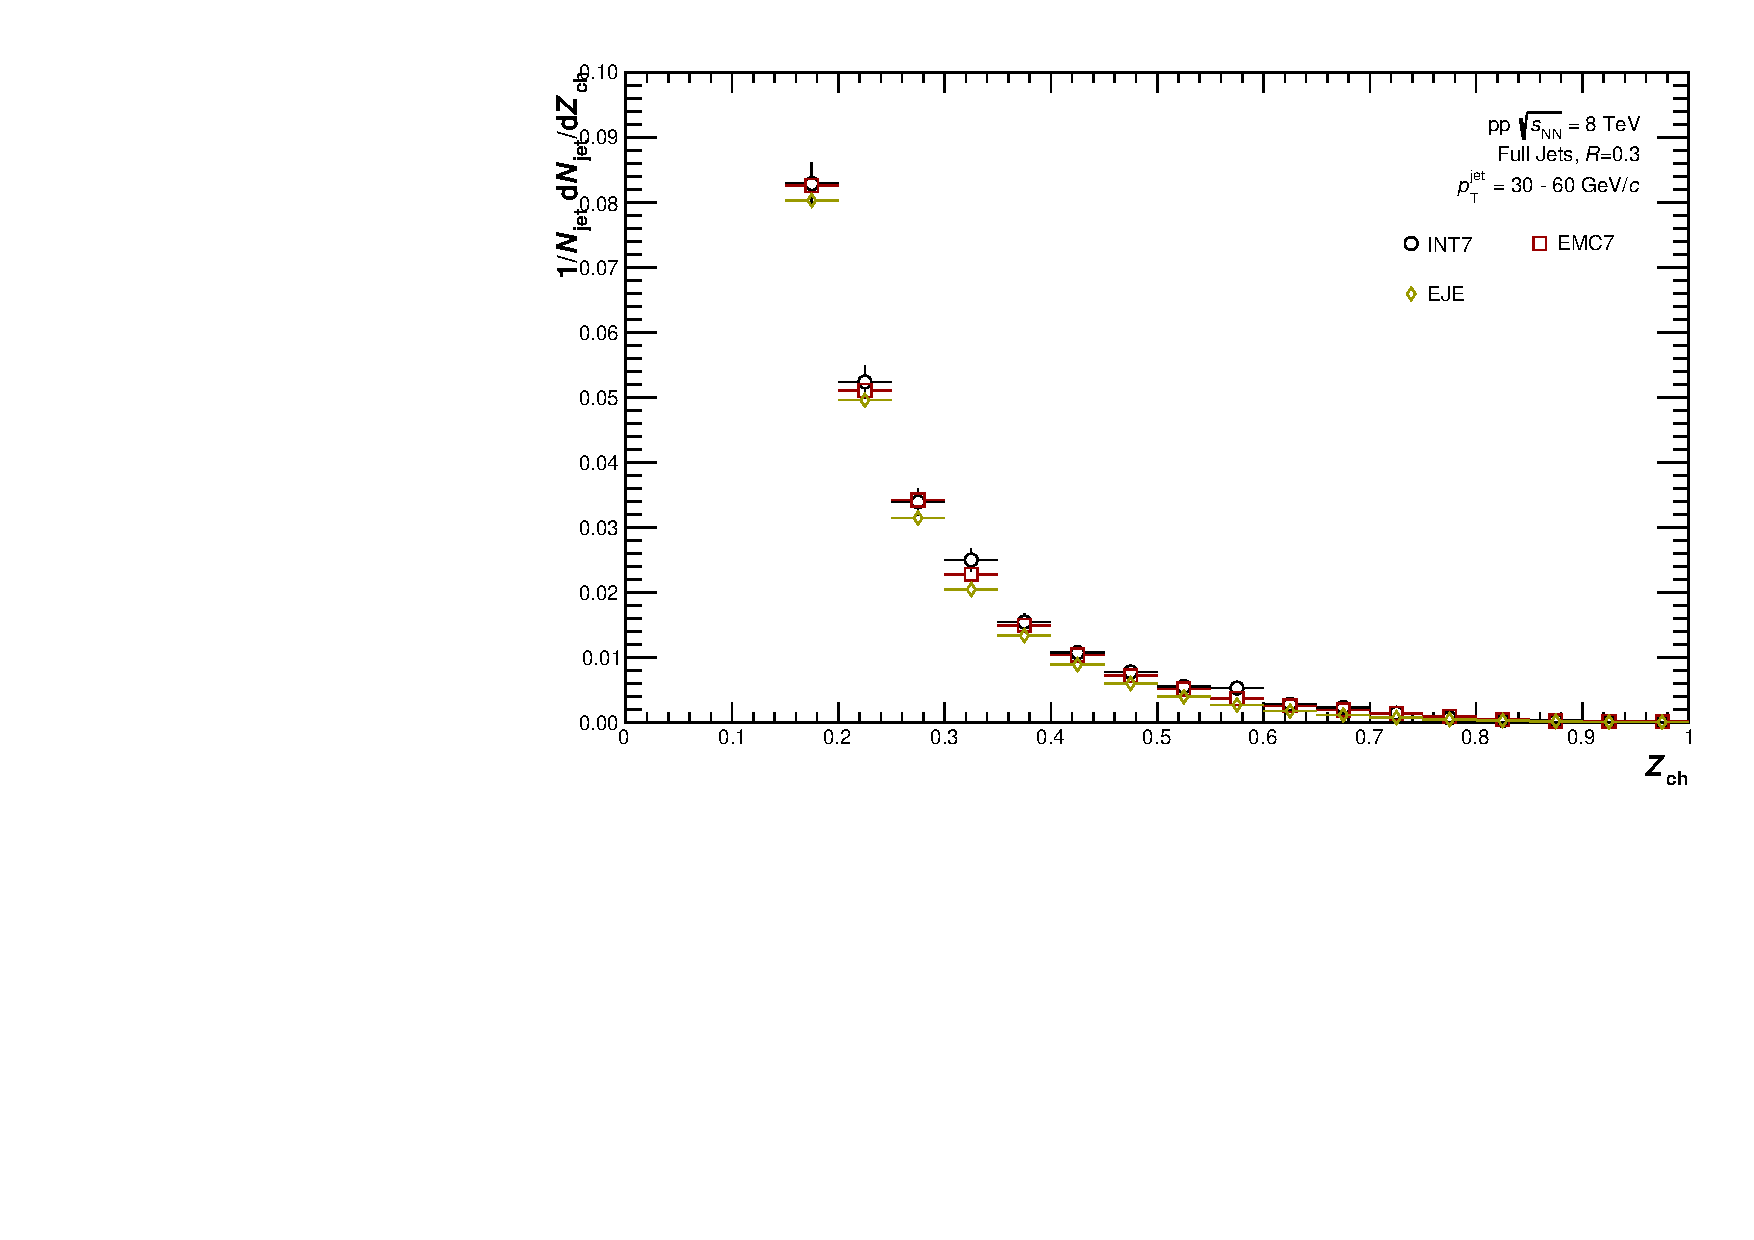
\includegraphics[width=.45\textwidth]{figures/Zch/All/hZch_30-60GeV_R03.pdf}}\\
    \subfigure{\label{fig:Zch_60-100GeV_R03}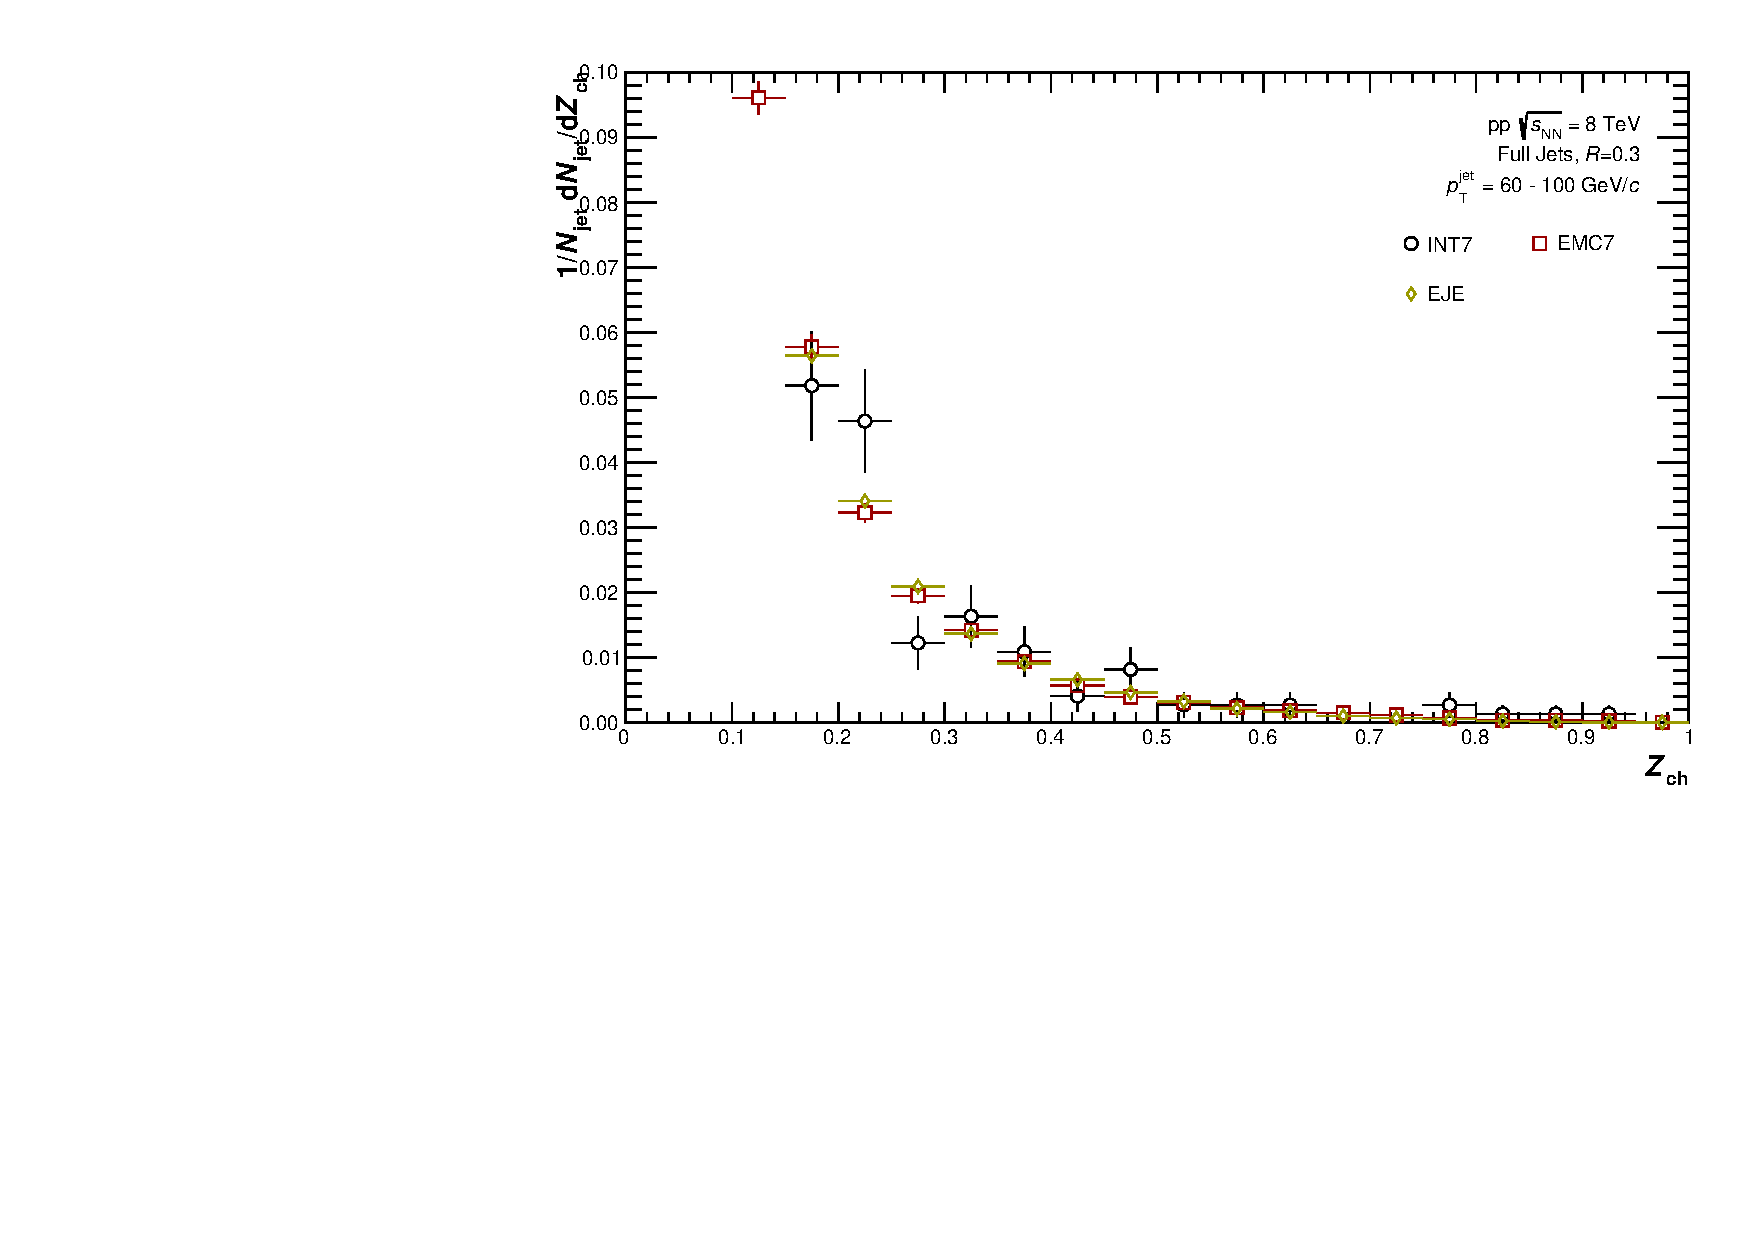
\includegraphics[width=.45\textwidth]{figures/Zch/All/hZch_60-100GeV_R03.pdf}}
    \qquad
    \subfigure{\label{fig:Zch_100-200GeV_R03}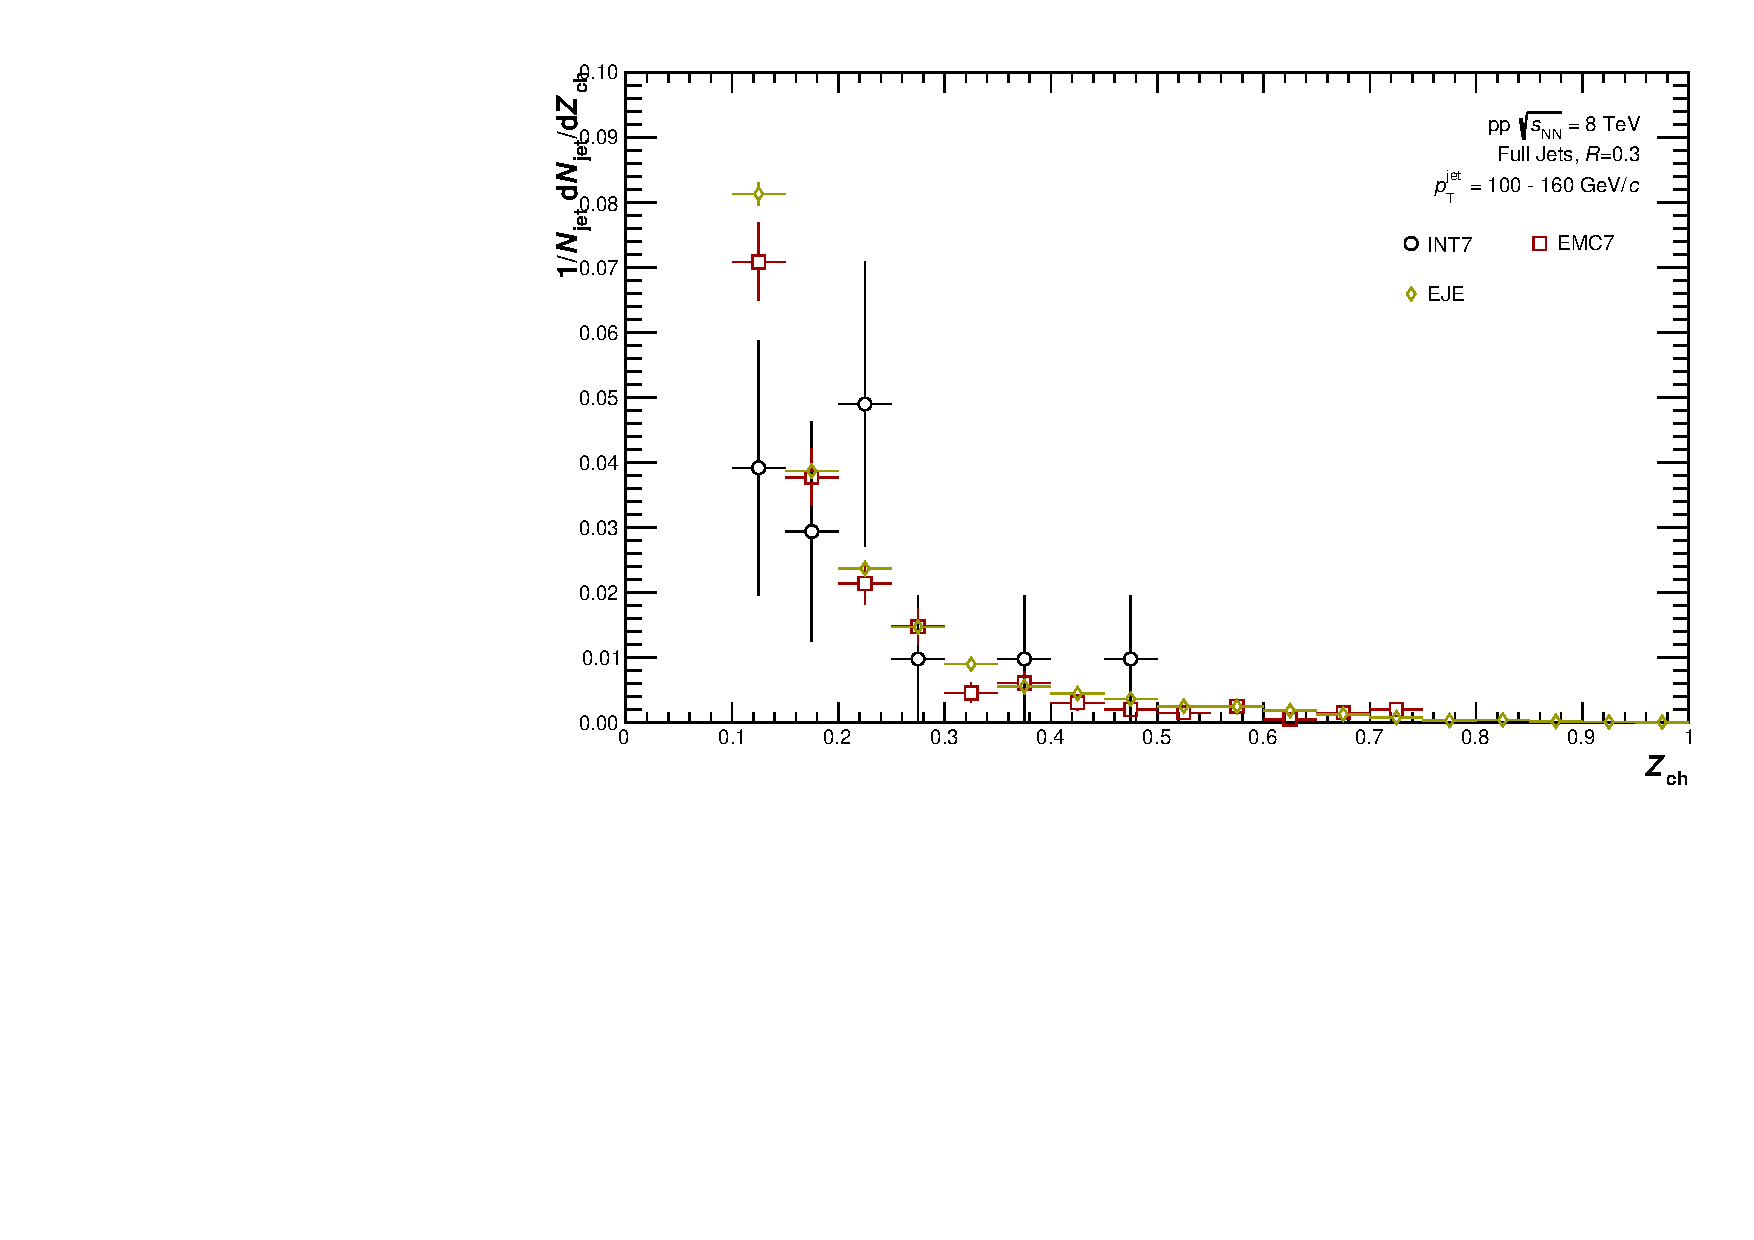
\includegraphics[width=.45\textwidth]{figures/Zch/All/hZch_100-160GeV_R03.pdf}}\\
    \subfigure{\label{fig:Zch_200-350GeV_R03}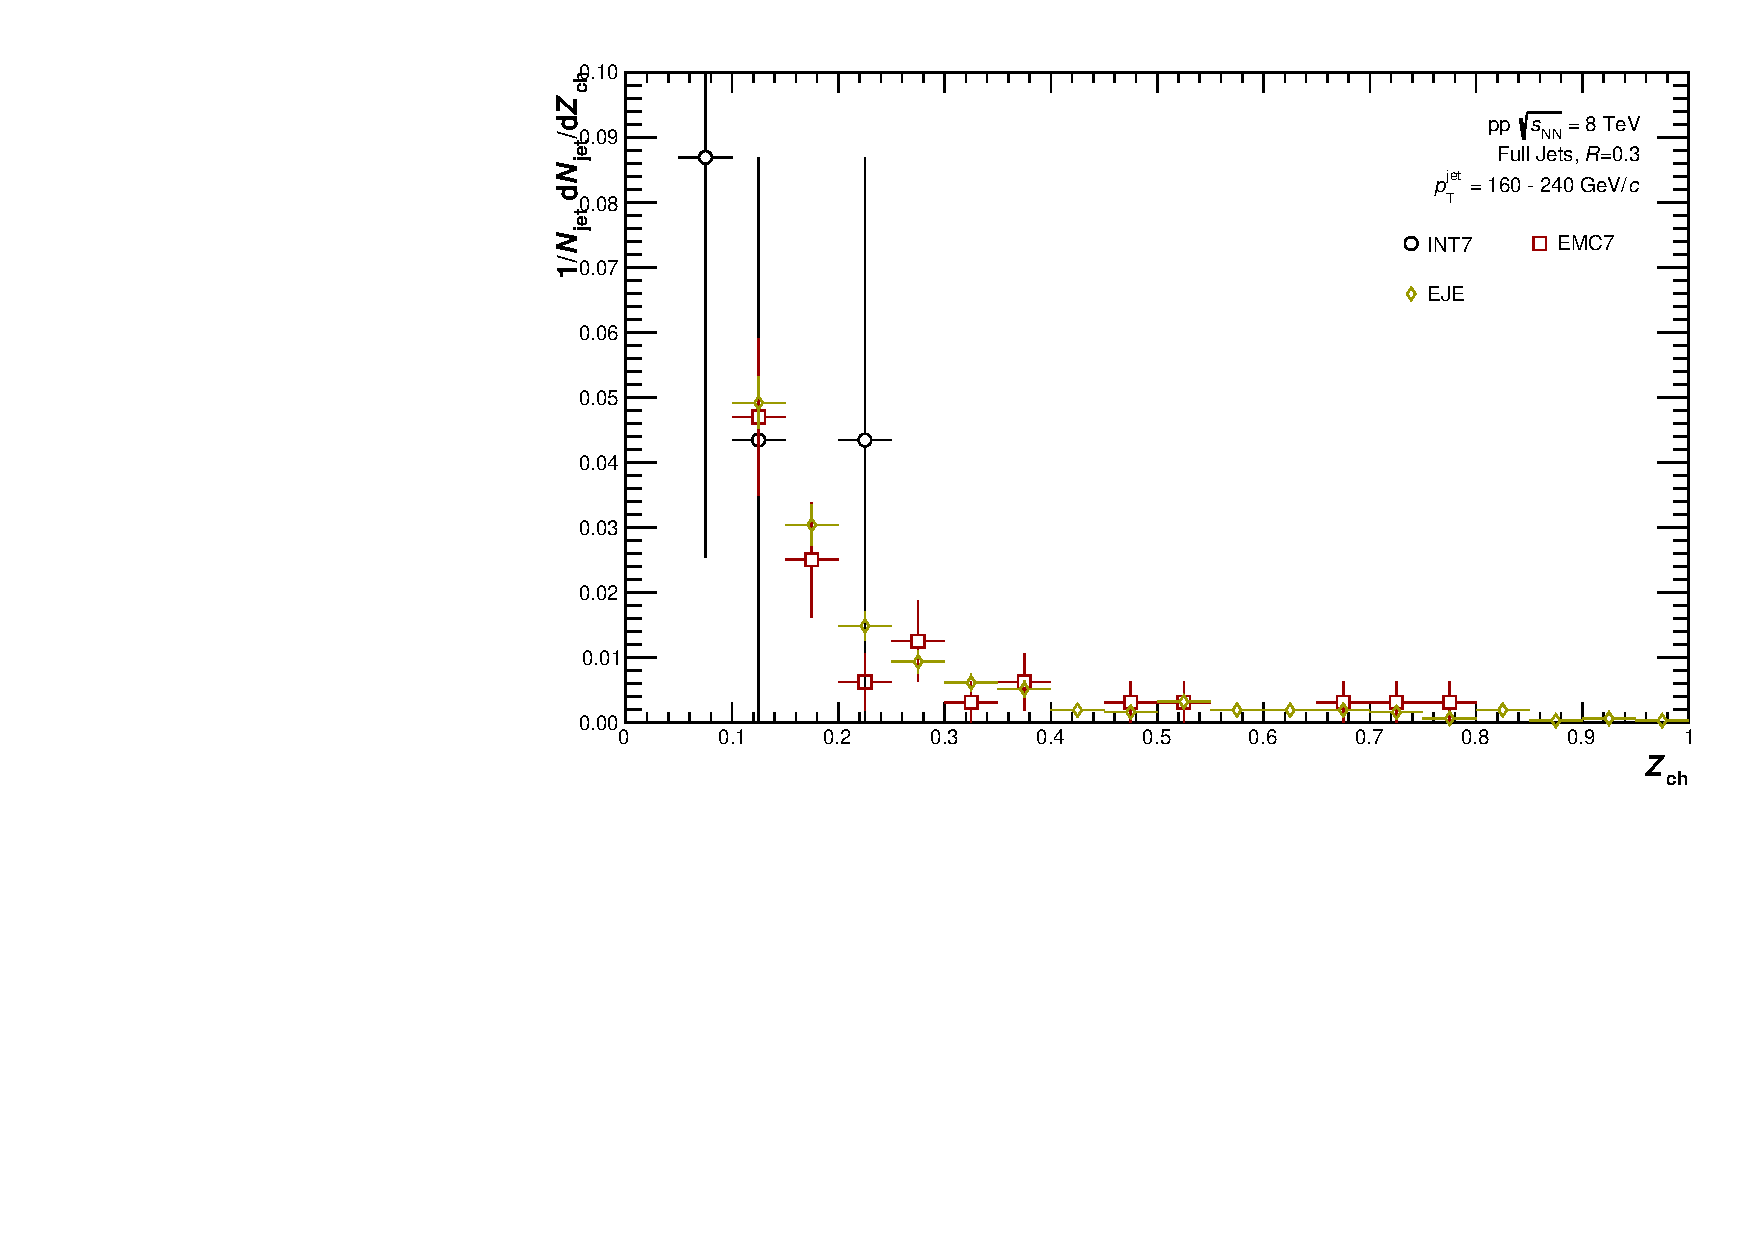
\includegraphics[width=.45\textwidth]{figures/Zch/All/hZch_160-240GeV_R03.pdf}}
    \caption{Z$_{ch}$ for R=0.3 jets in several bins of \pT}
    \label{fig:TriggerBiasZchR03}
\end{figure}

\newpage

\begin{figure}[h!]
    \centering
    \subfigure{\label{fig:Zne_6-10GeV_R03}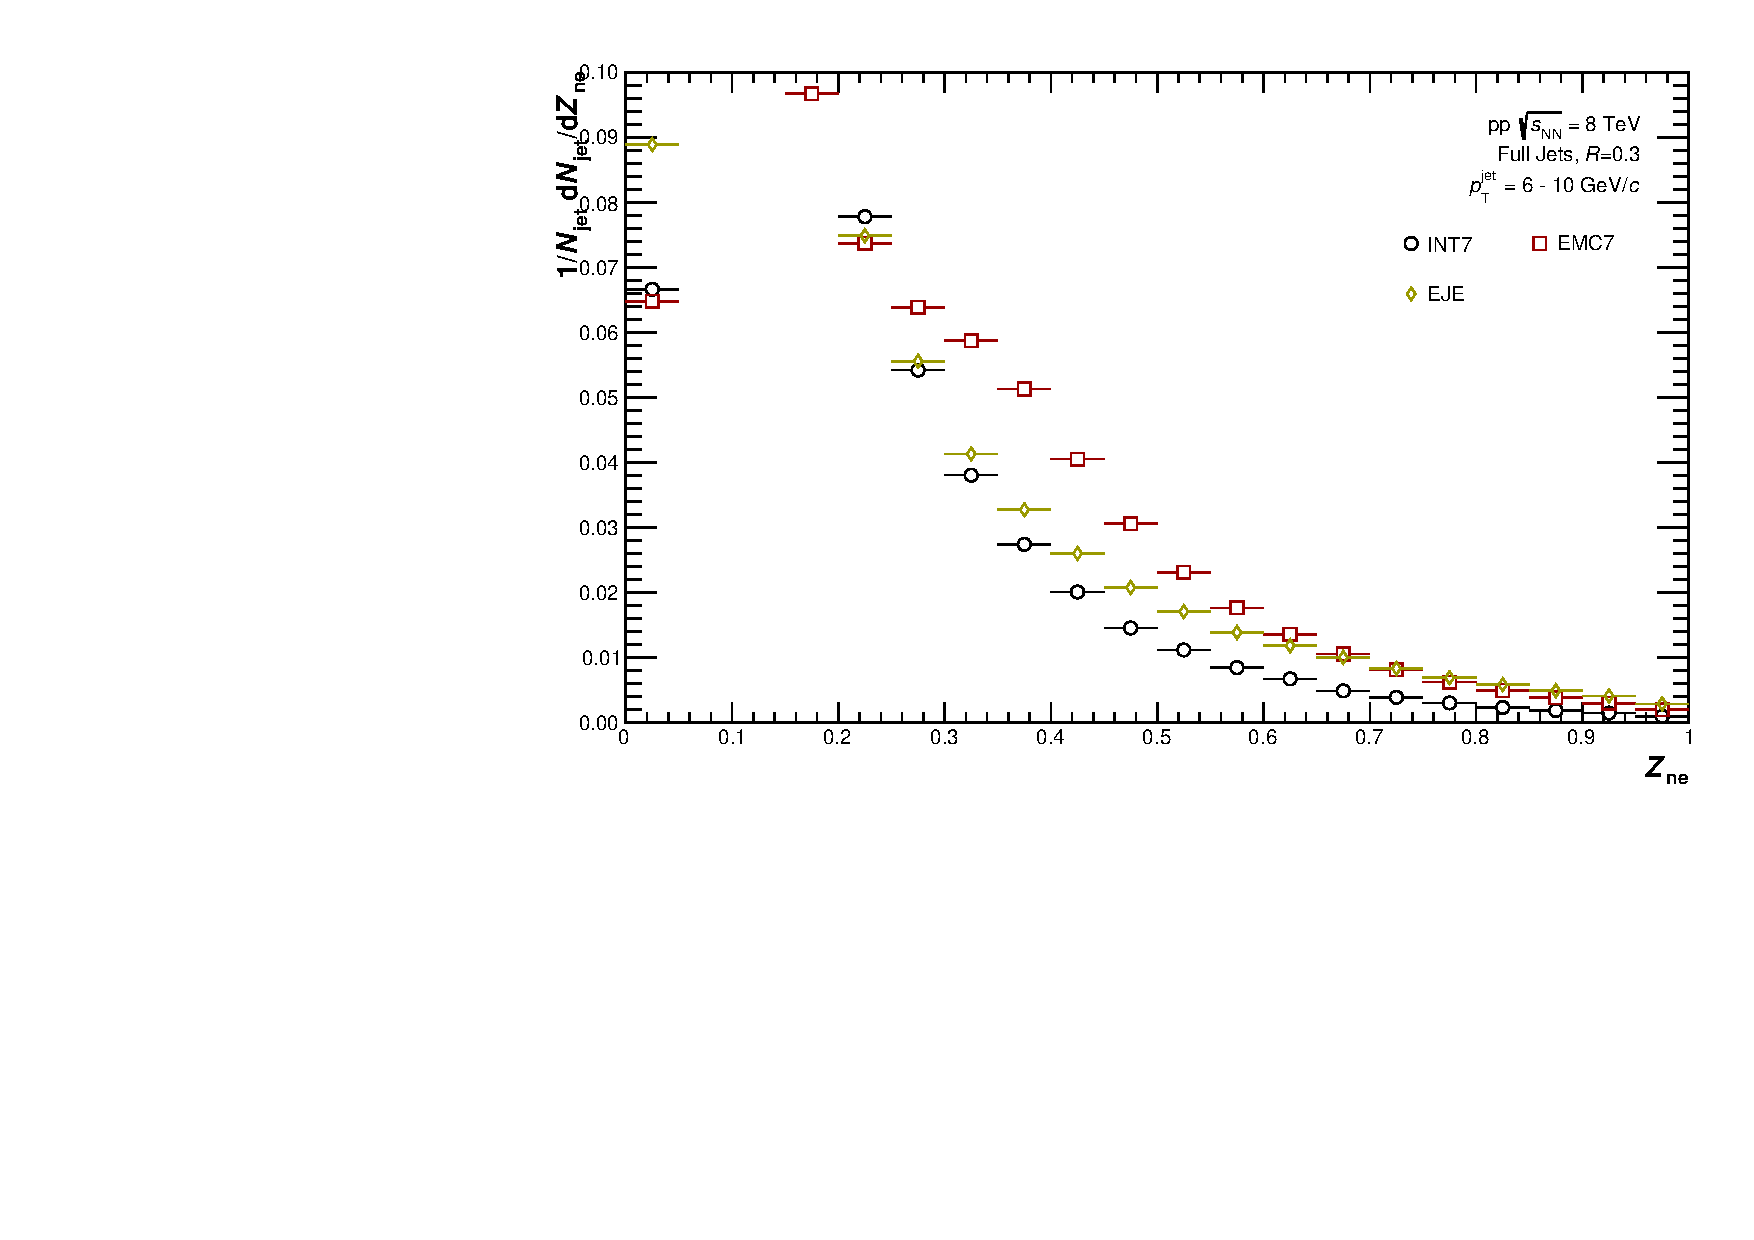
\includegraphics[width=.45\textwidth]{figures/Zne/All/hZne_6-10GeV_R03.pdf}}
    \qquad
    \subfigure{\label{fig:Zne_10-20GeV_R03}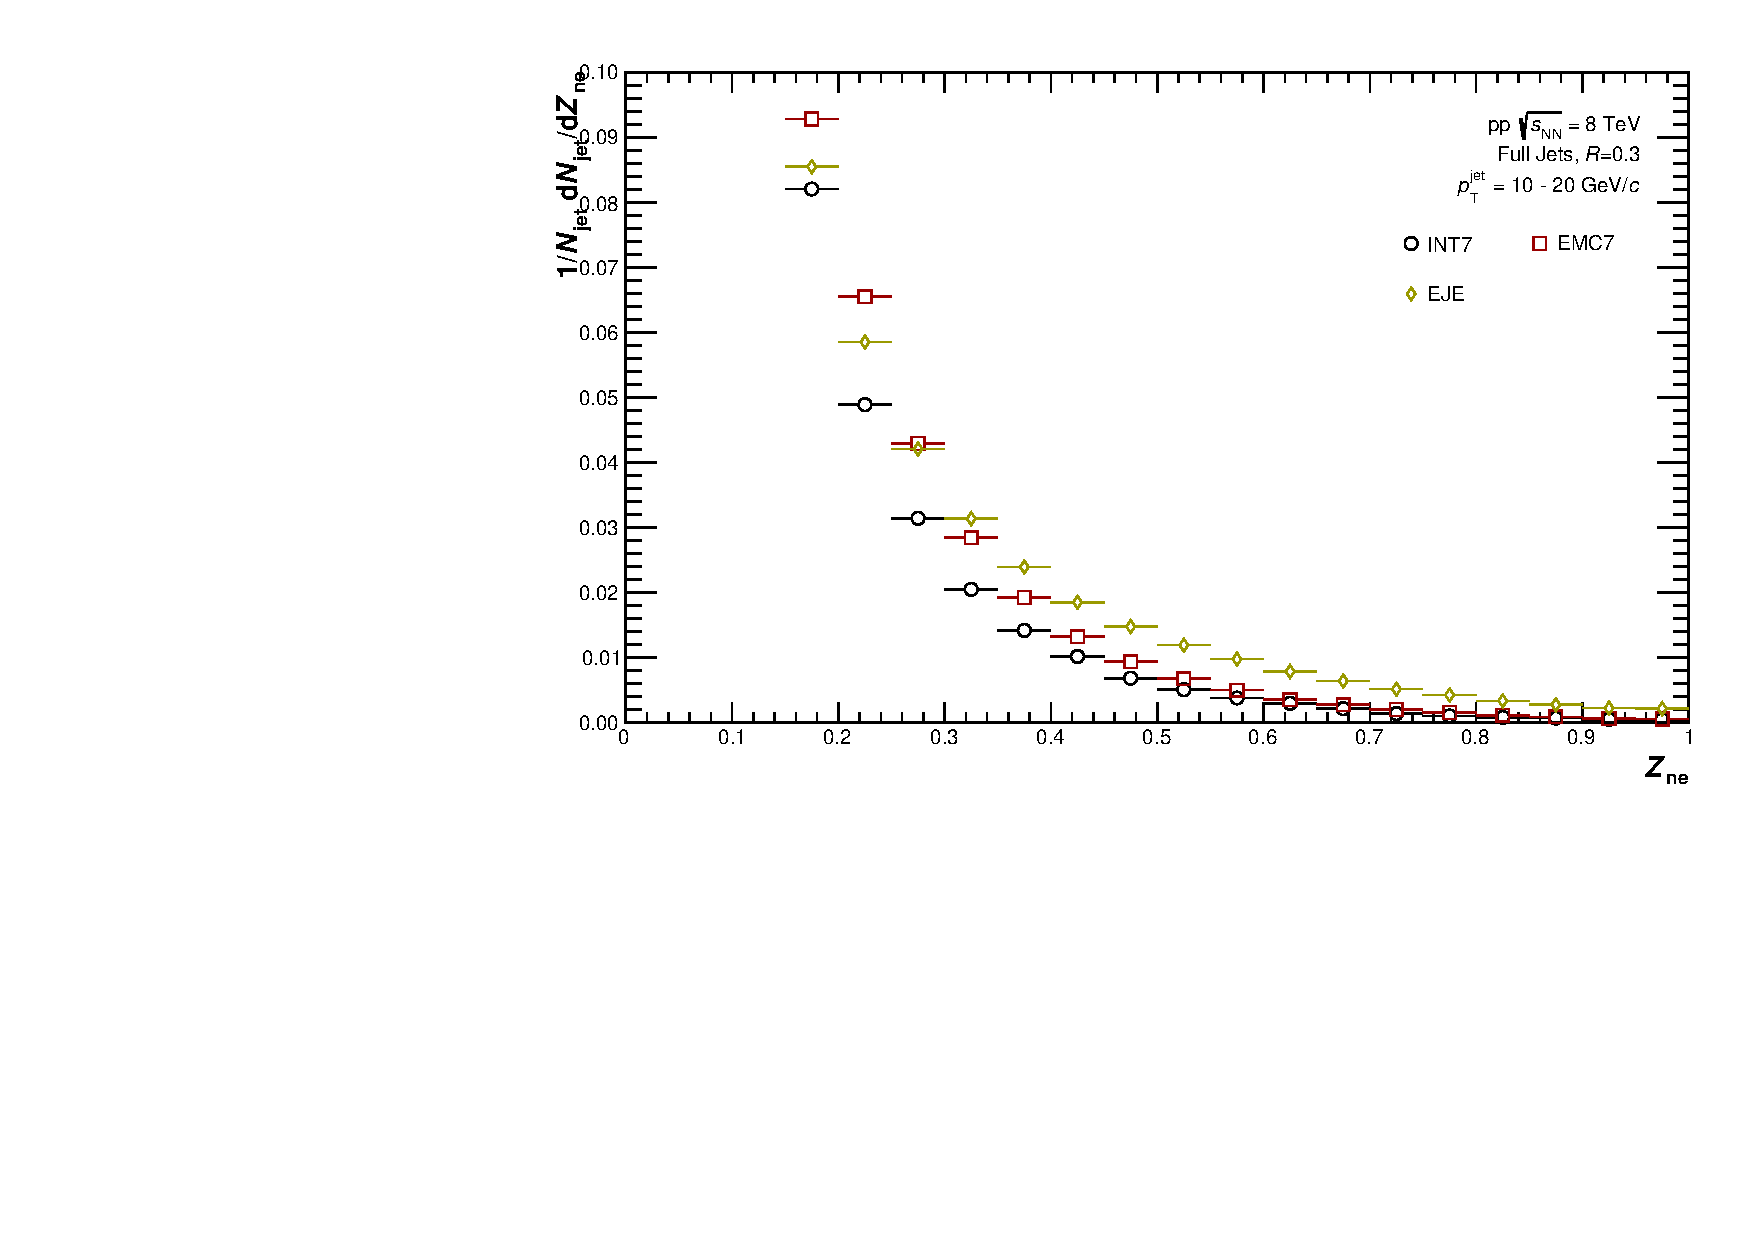
\includegraphics[width=.45\textwidth]{figures/Zne/All/hZne_10-20GeV_R03.pdf}}\\
    \subfigure{\label{fig:Zne_20-30GeV_R03}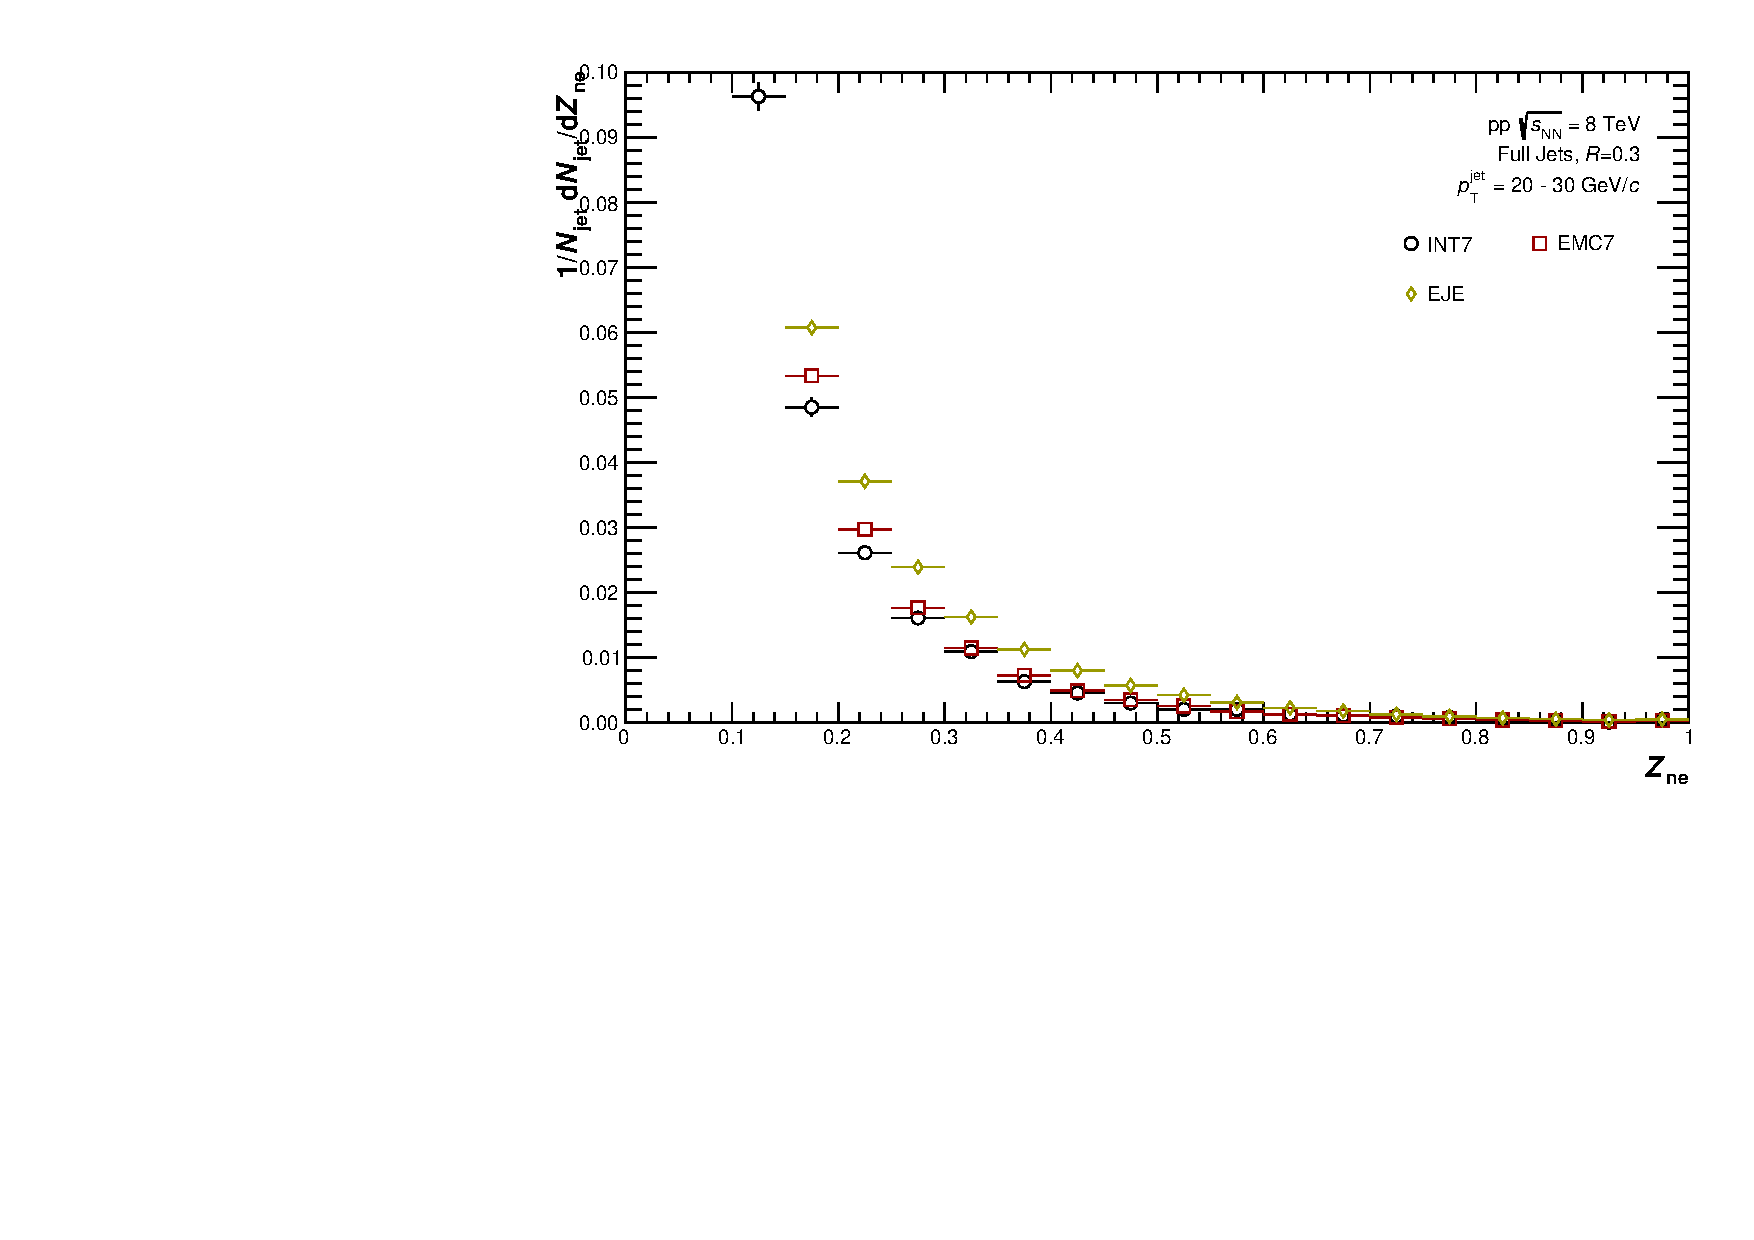
\includegraphics[width=.45\textwidth]{figures/Zne/All/hZne_20-30GeV_R03.pdf}}
    \qquad
    \subfigure{\label{fig:Zne_30-60GeV_R03}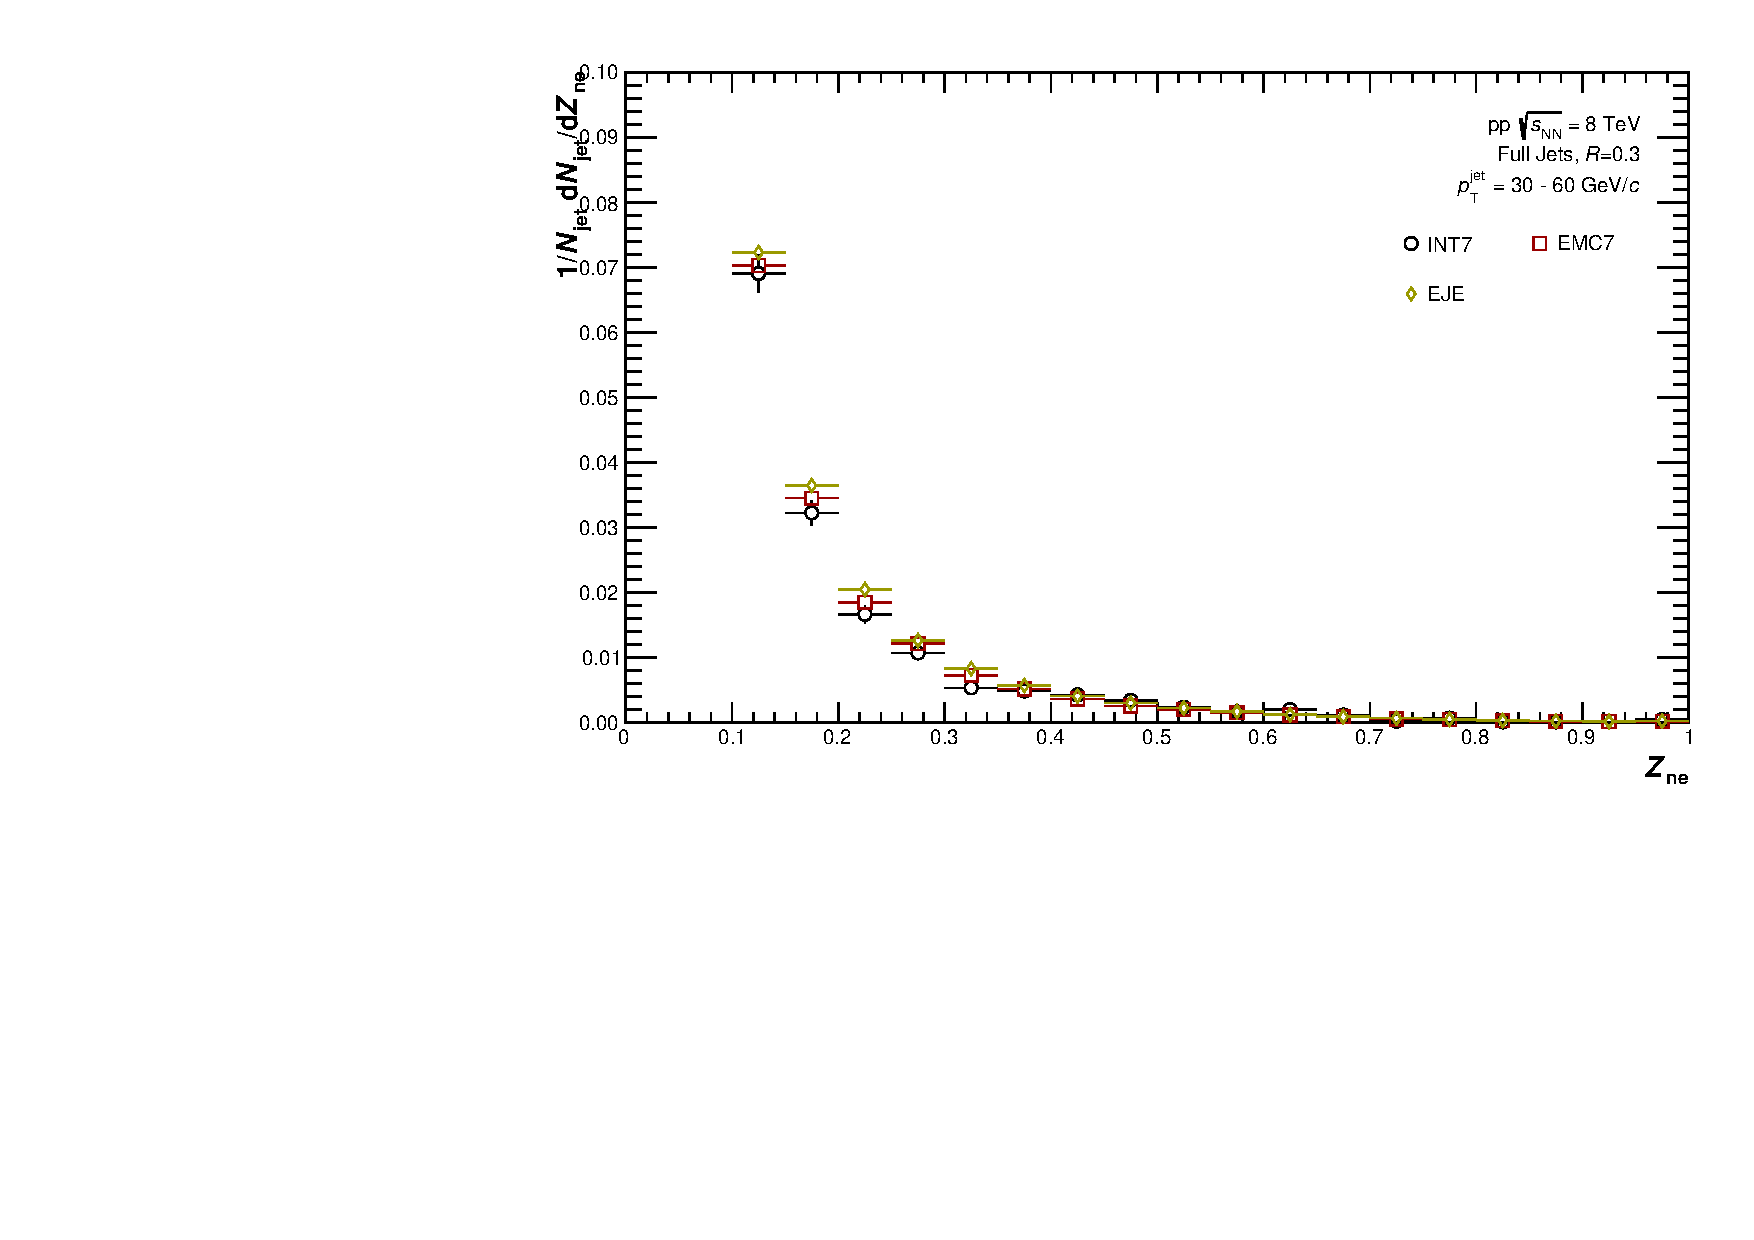
\includegraphics[width=.45\textwidth]{figures/Zne/All/hZne_30-60GeV_R03.pdf}}\\
    \subfigure{\label{fig:Zne_60-100GeV_R03}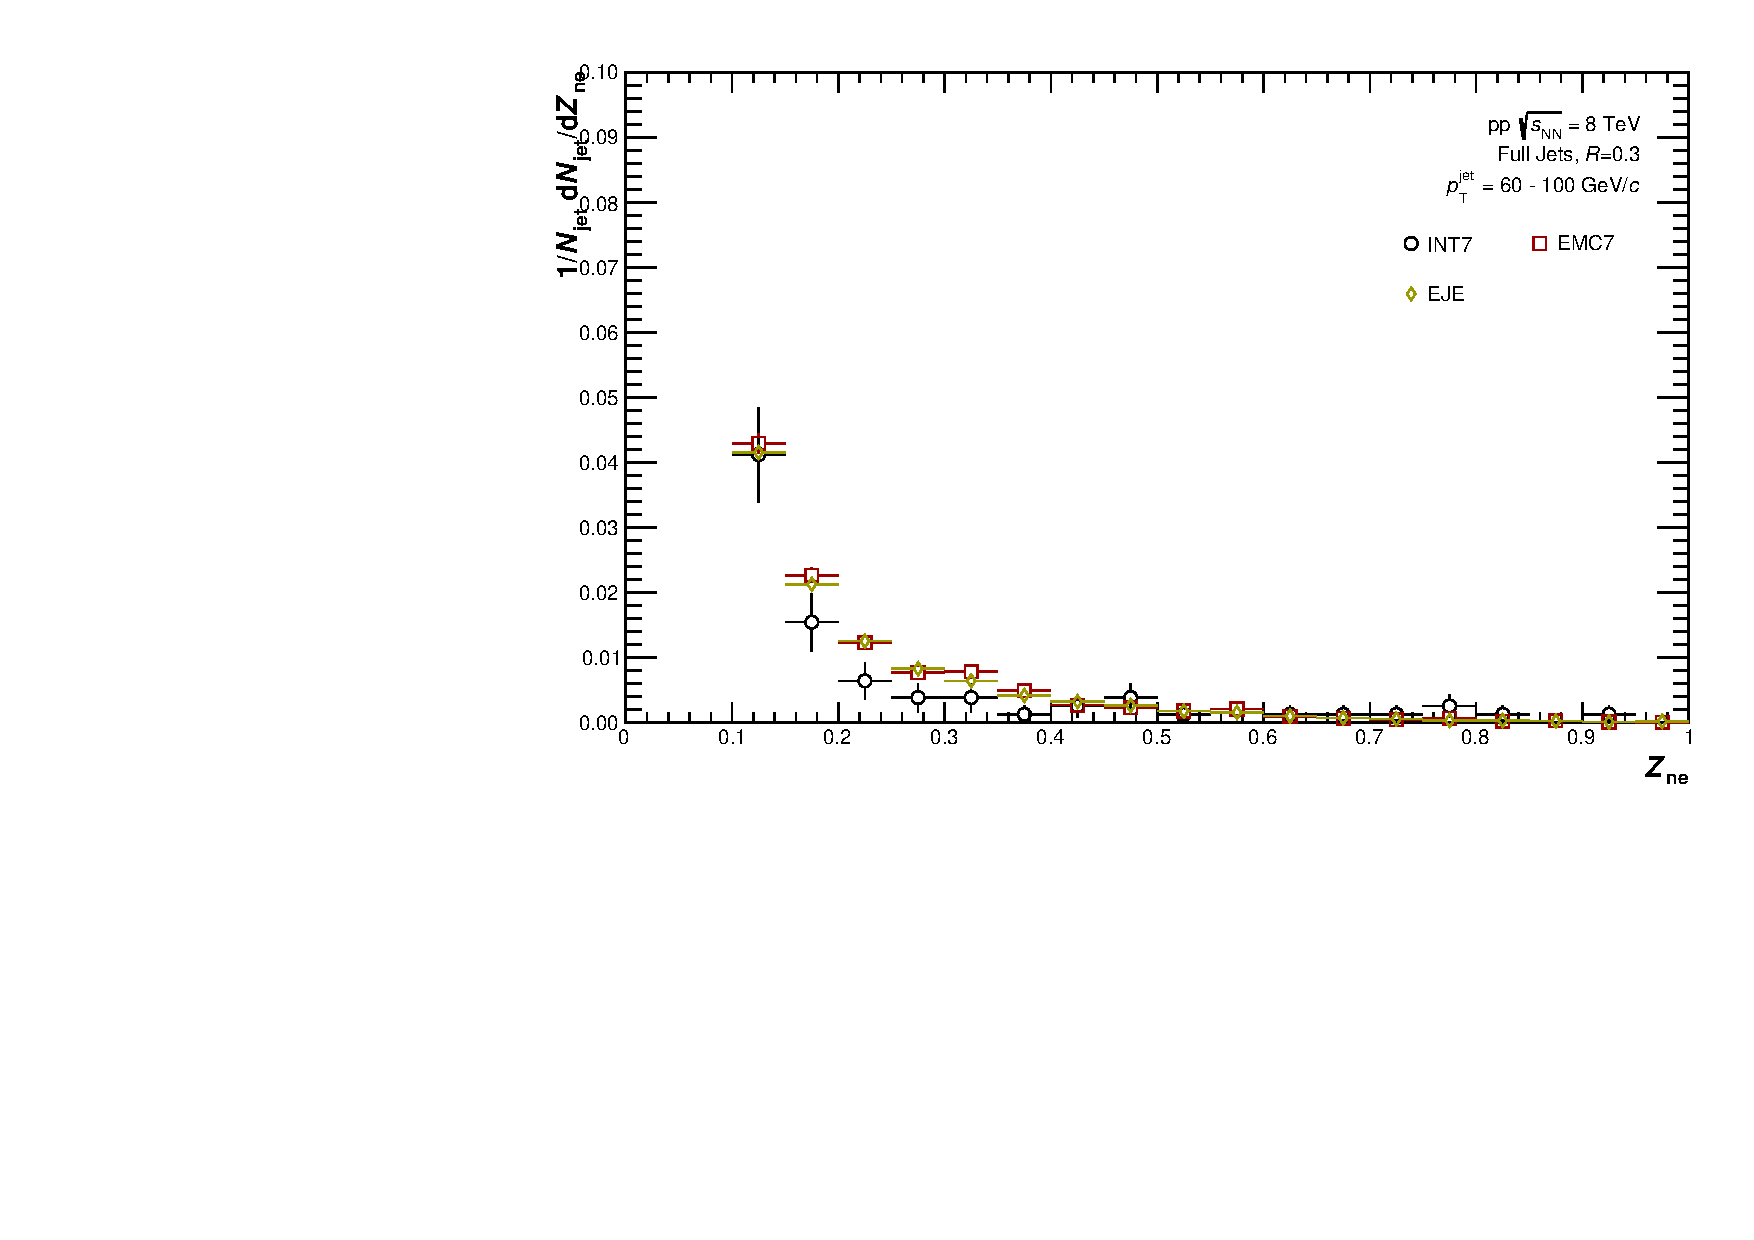
\includegraphics[width=.45\textwidth]{figures/Zne/All/hZne_60-100GeV_R03.pdf}}
    \qquad
    \subfigure{\label{fig:Zne_100-200GeV_R03}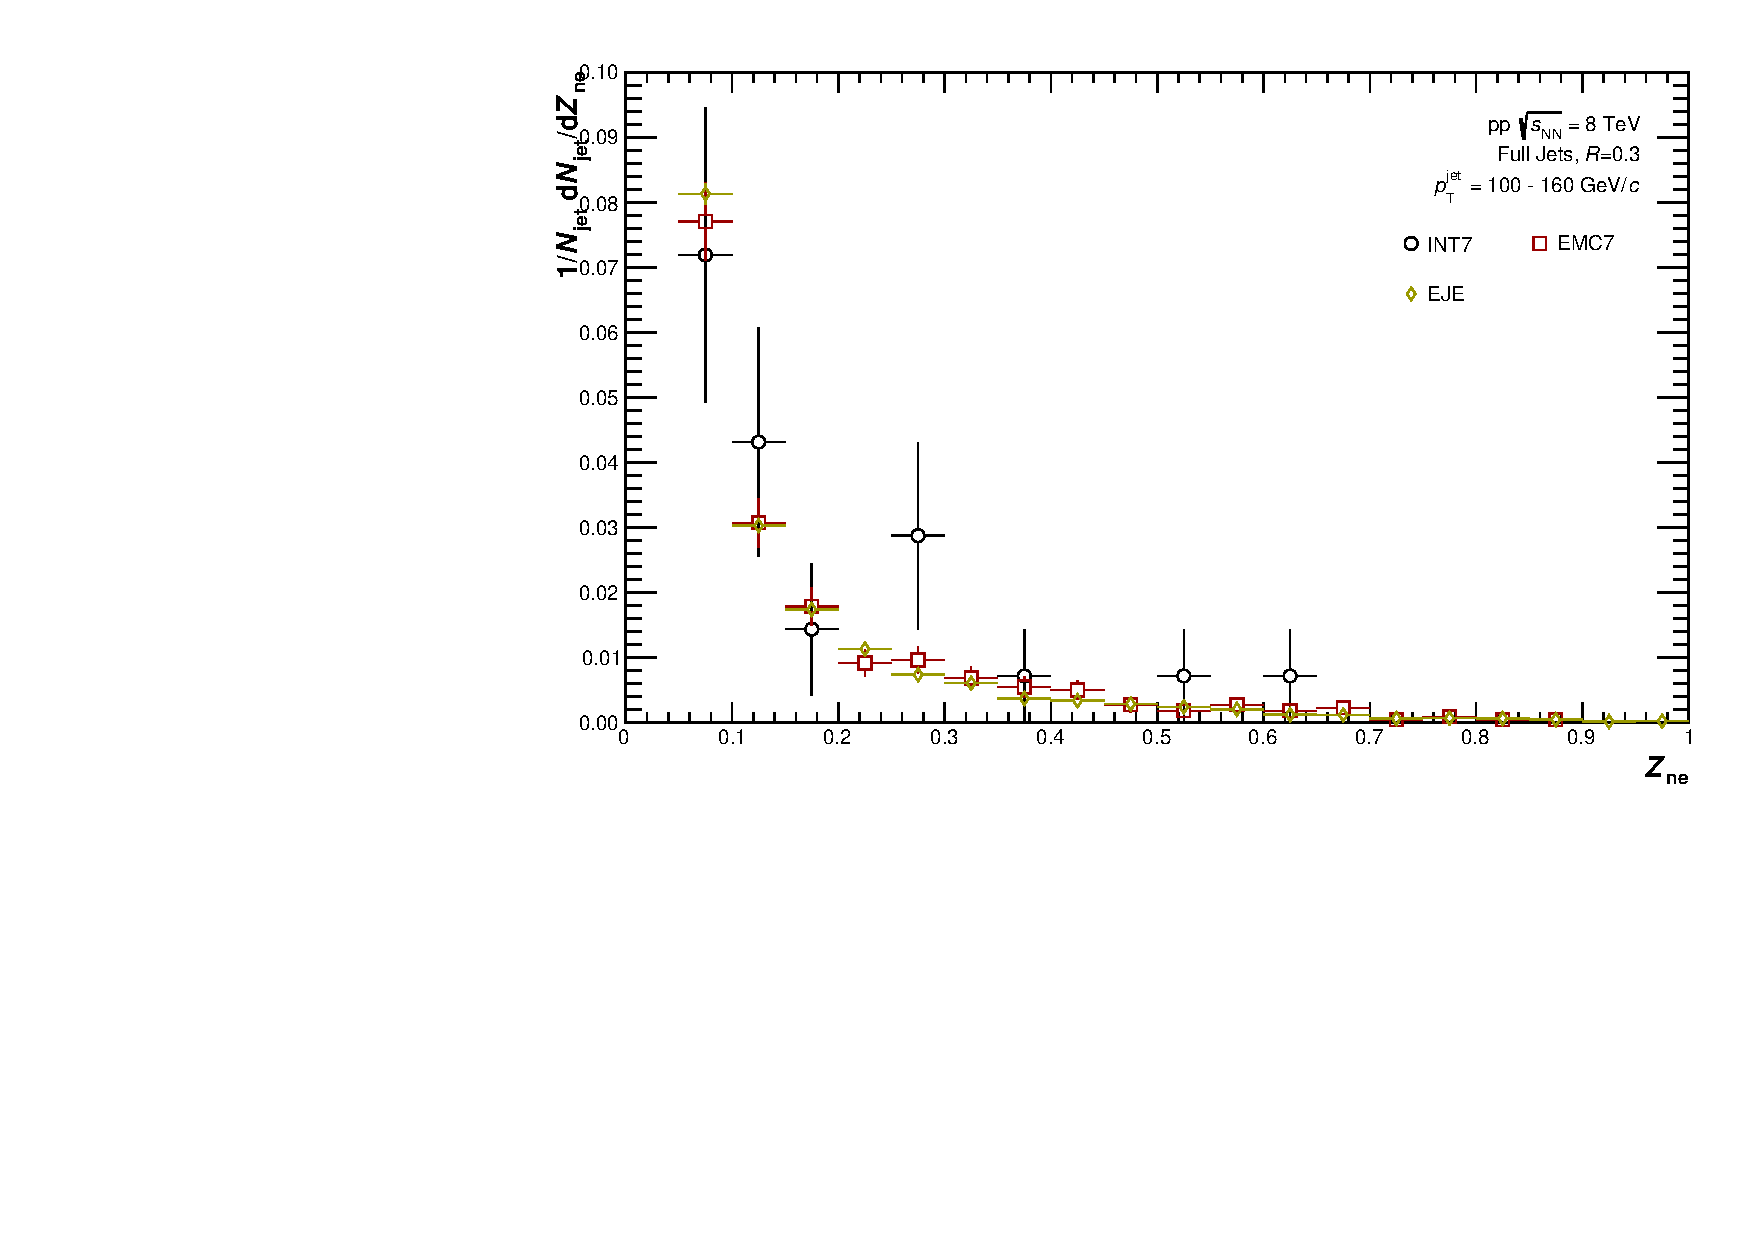
\includegraphics[width=.45\textwidth]{figures/Zne/All/hZne_100-160GeV_R03.pdf}}\\
    \subfigure{\label{fig:Zne_200-350GeV_R03}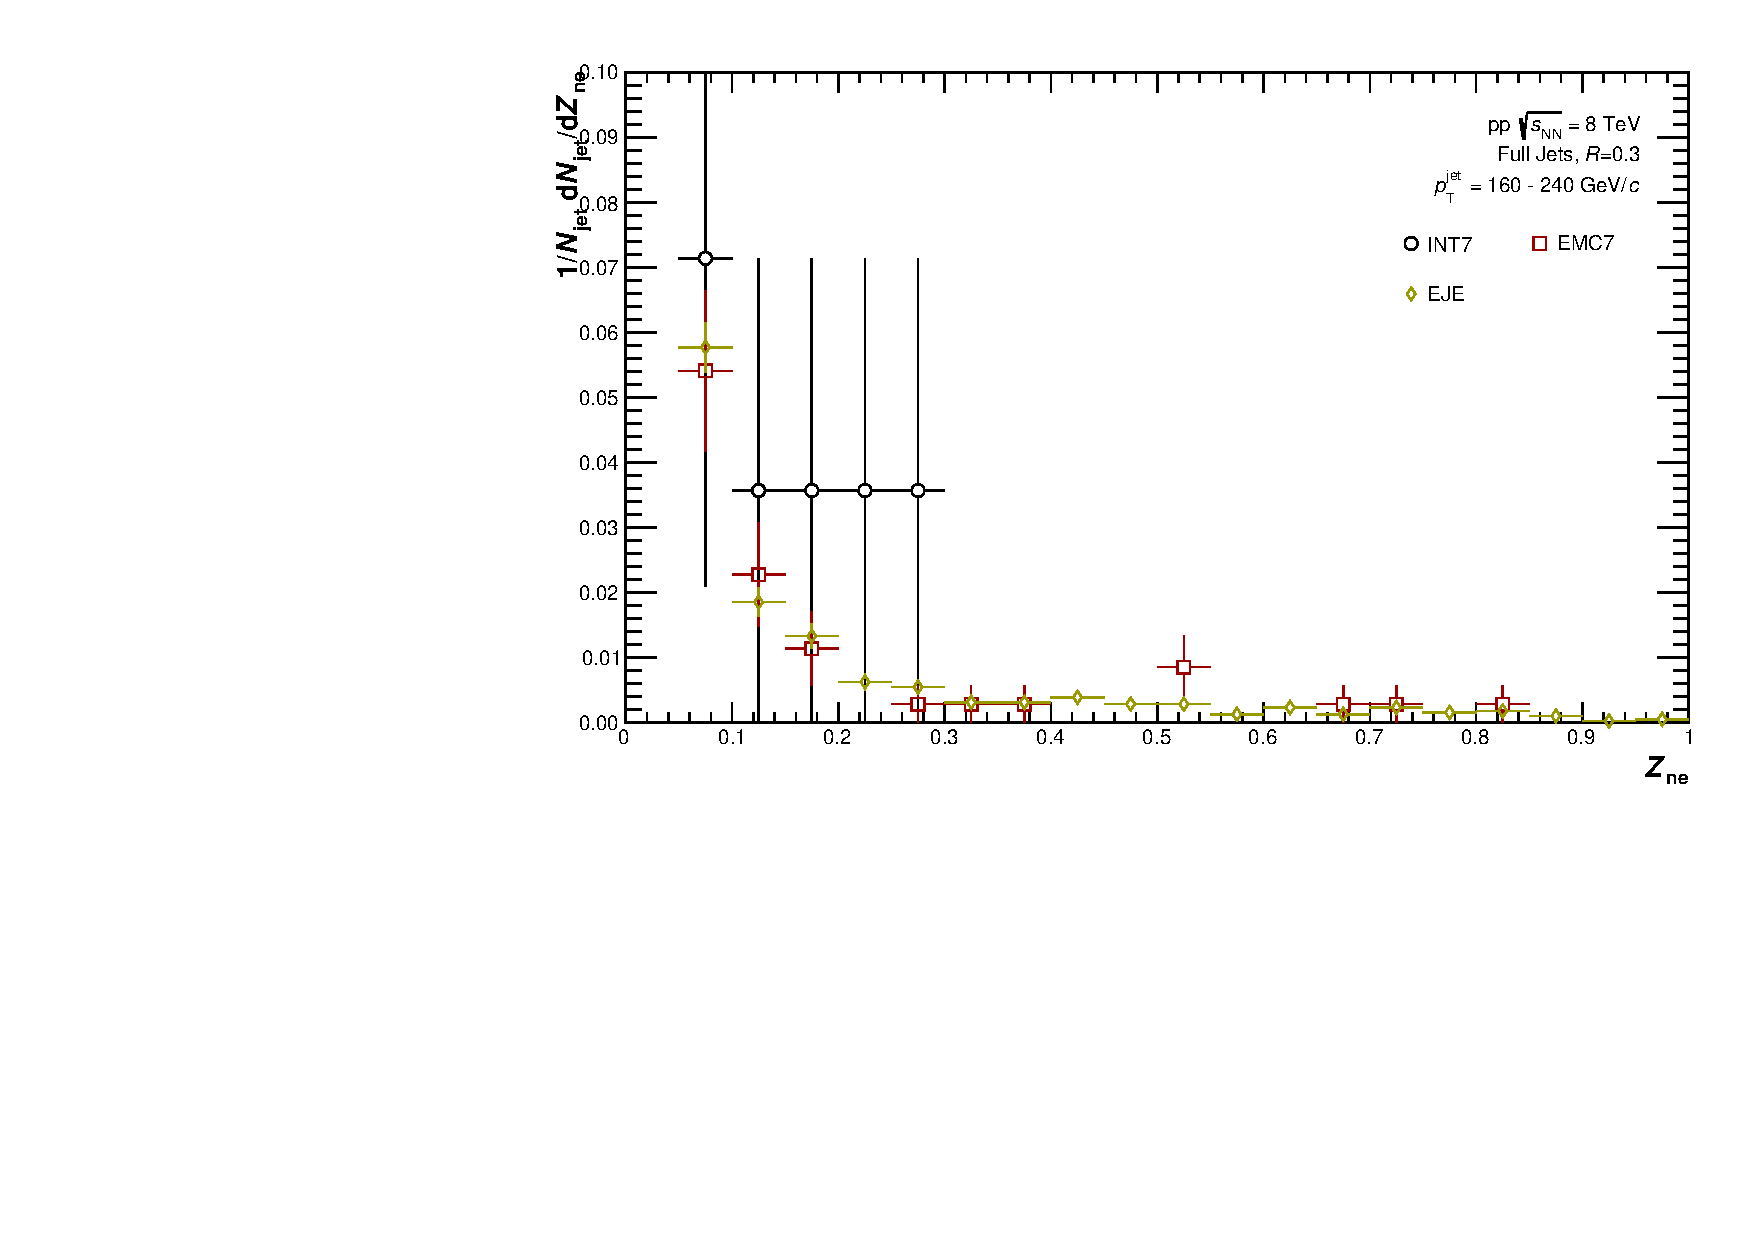
\includegraphics[width=.45\textwidth]{figures/Zne/All/hZne_160-240GeV_R03.pdf}}
    \caption{Z$_{ne}$ for R=0.3 jets in several bins of \pT}
    \label{fig:TriggerBiasZneR03}
\end{figure}

%%%%%%%%%%%%%%%%%%%%%%%%%%%%%%% R=0.4
\newpage

\begin{figure}[h!]
    \centering
    \subfigure{\label{fig:NEF_6-10GeV_R04}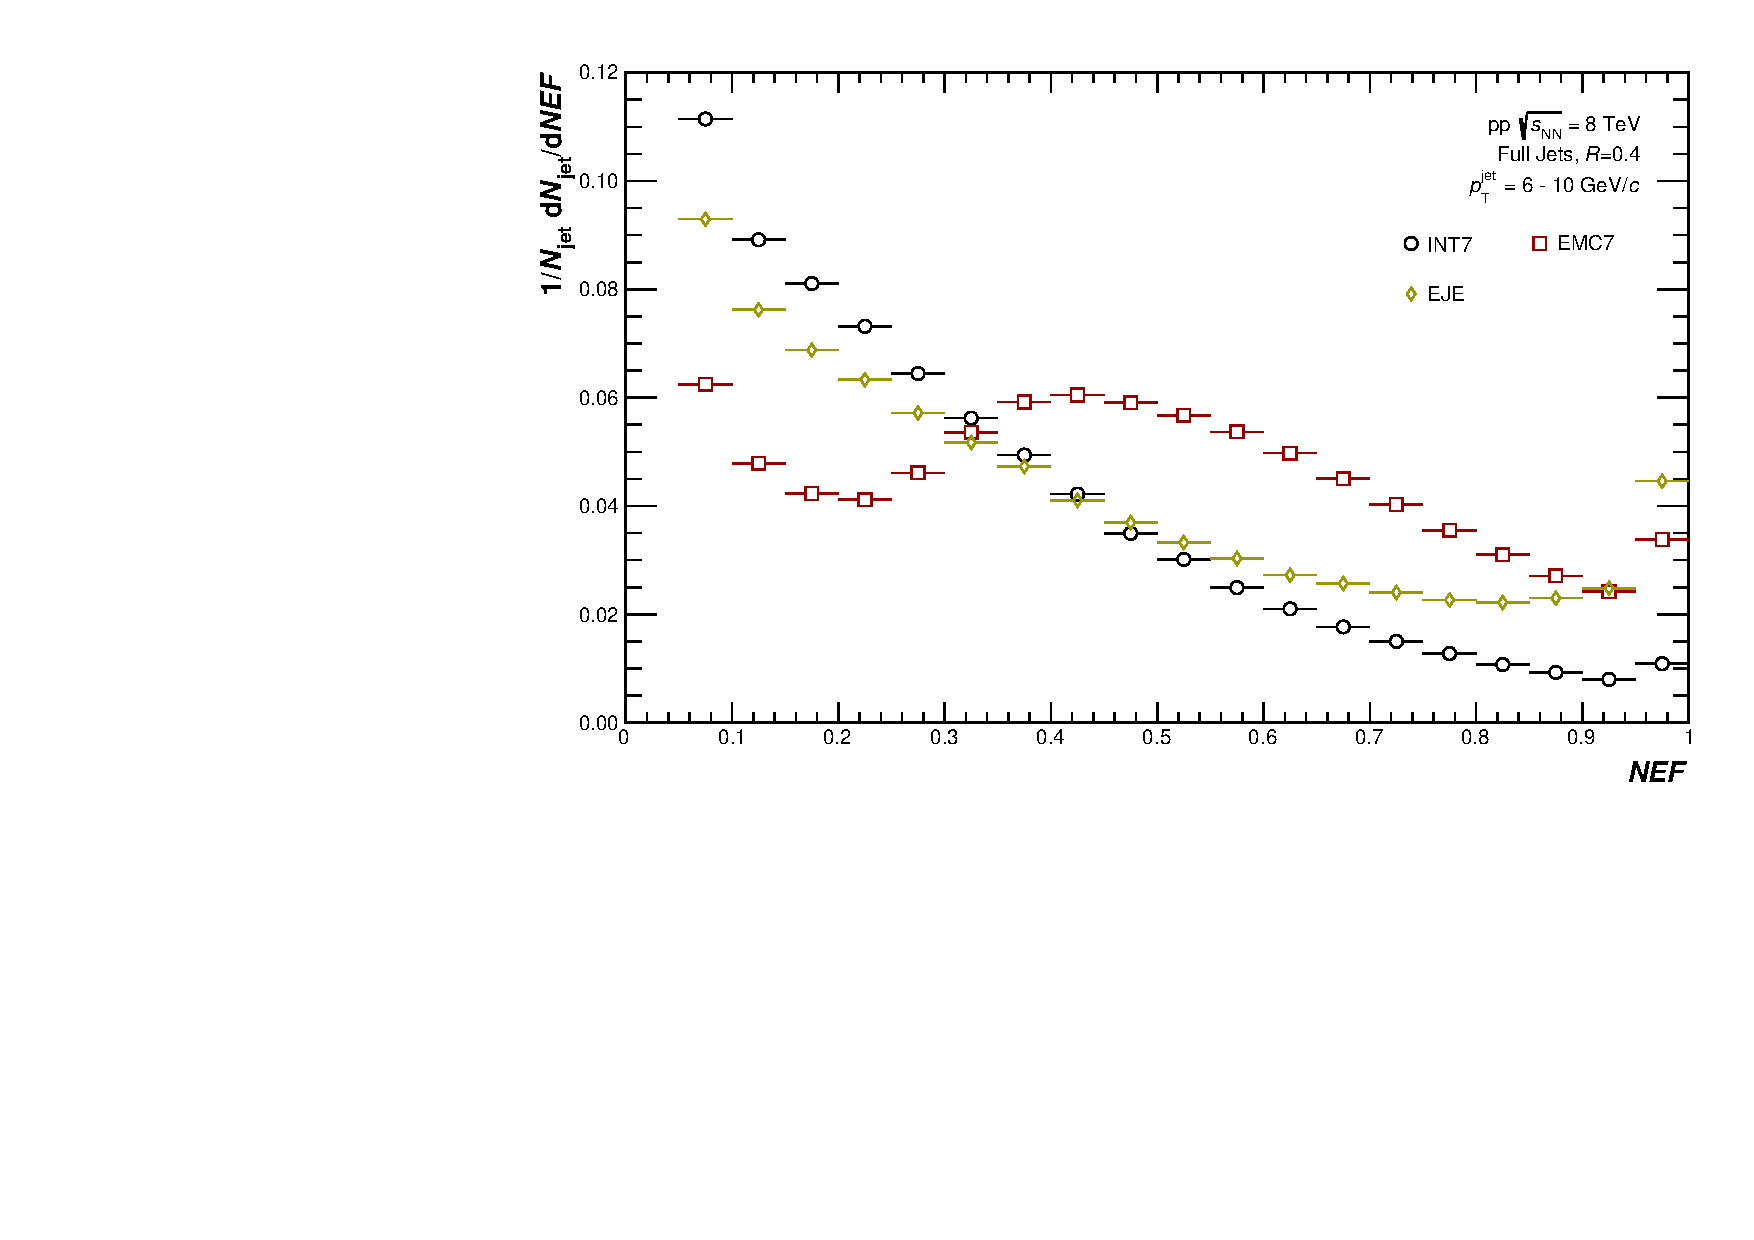
\includegraphics[width=.45\textwidth]{figures/NEF/All/hNEF_6-10GeV_R04.pdf}}
    \qquad
    \subfigure{\label{fig:NEF_10-20GeV_R04}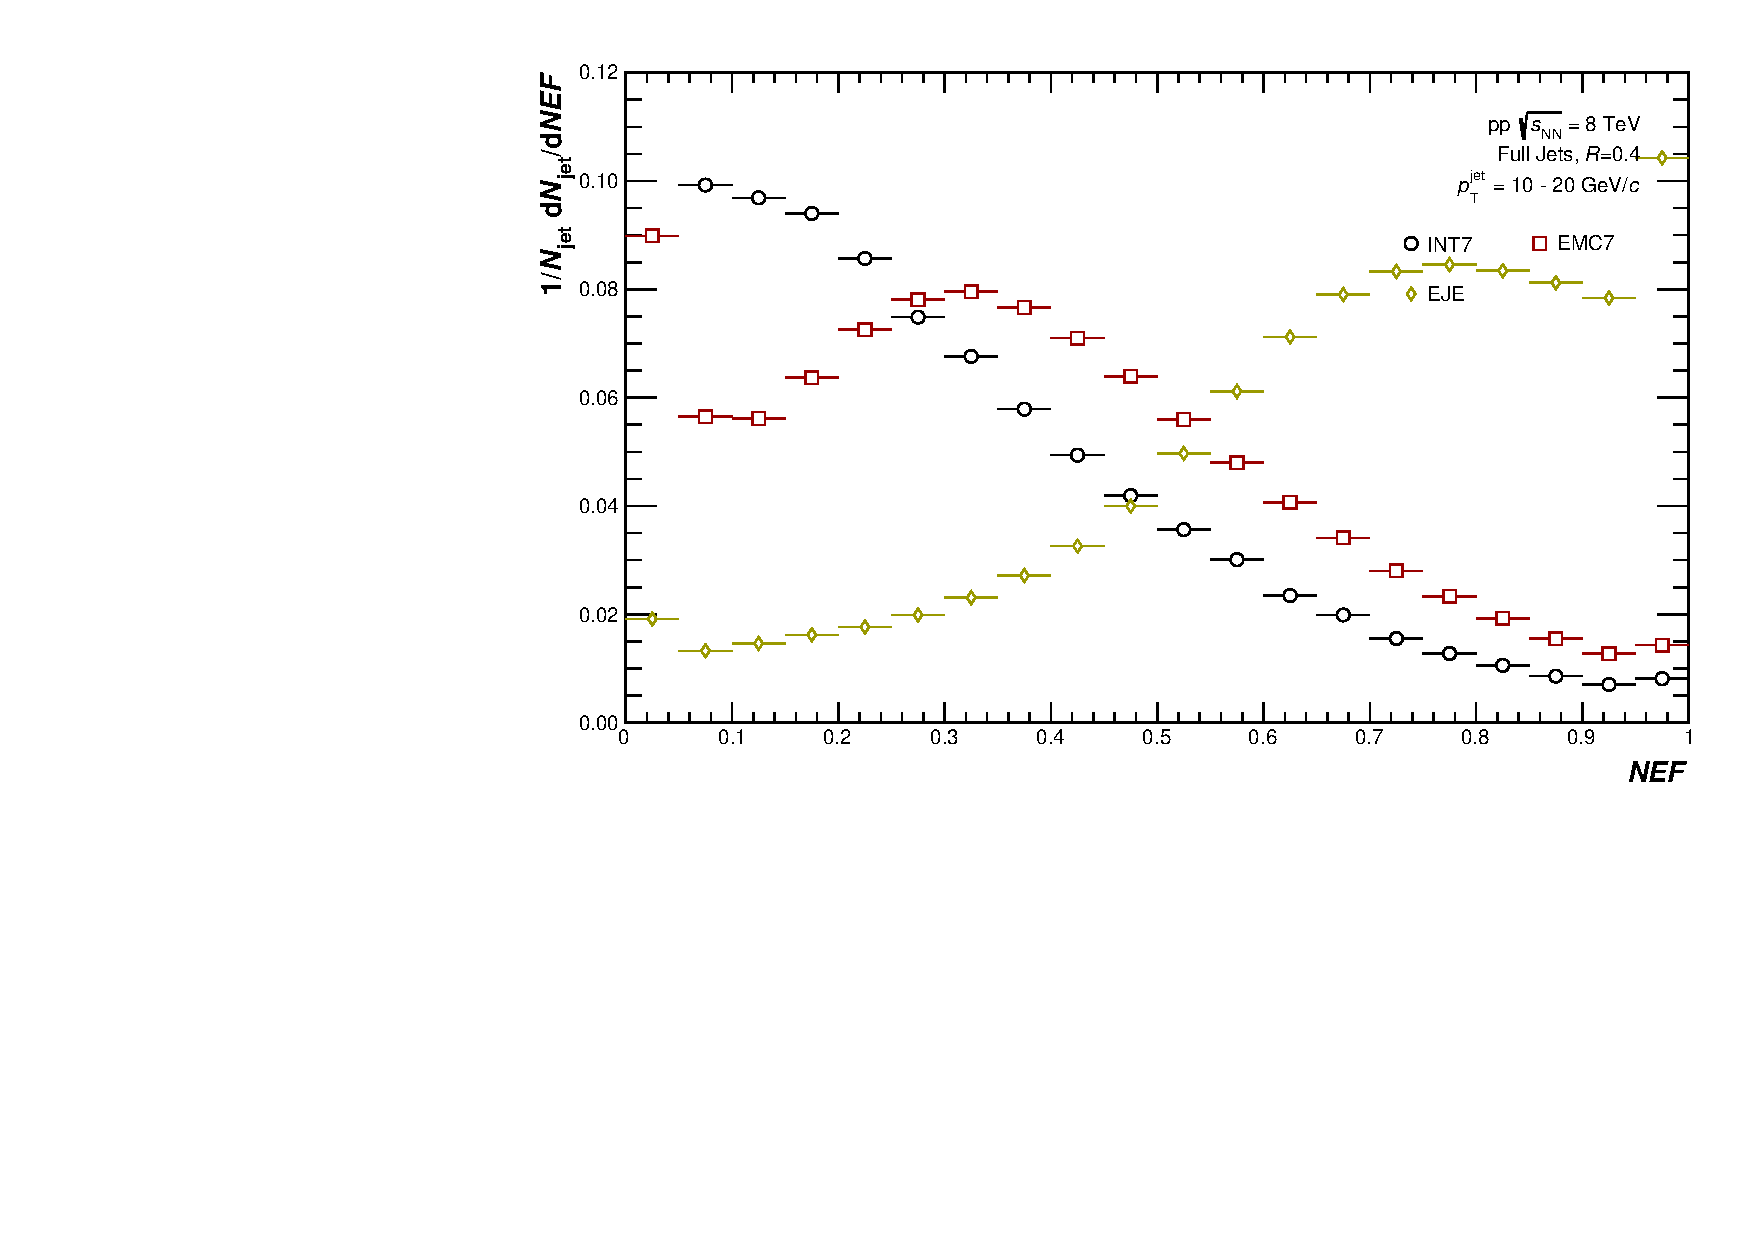
\includegraphics[width=.45\textwidth]{figures/NEF/All/hNEF_10-20GeV_R04.pdf}}\\
    \subfigure{\label{fig:NEF_20-30GeV_R04}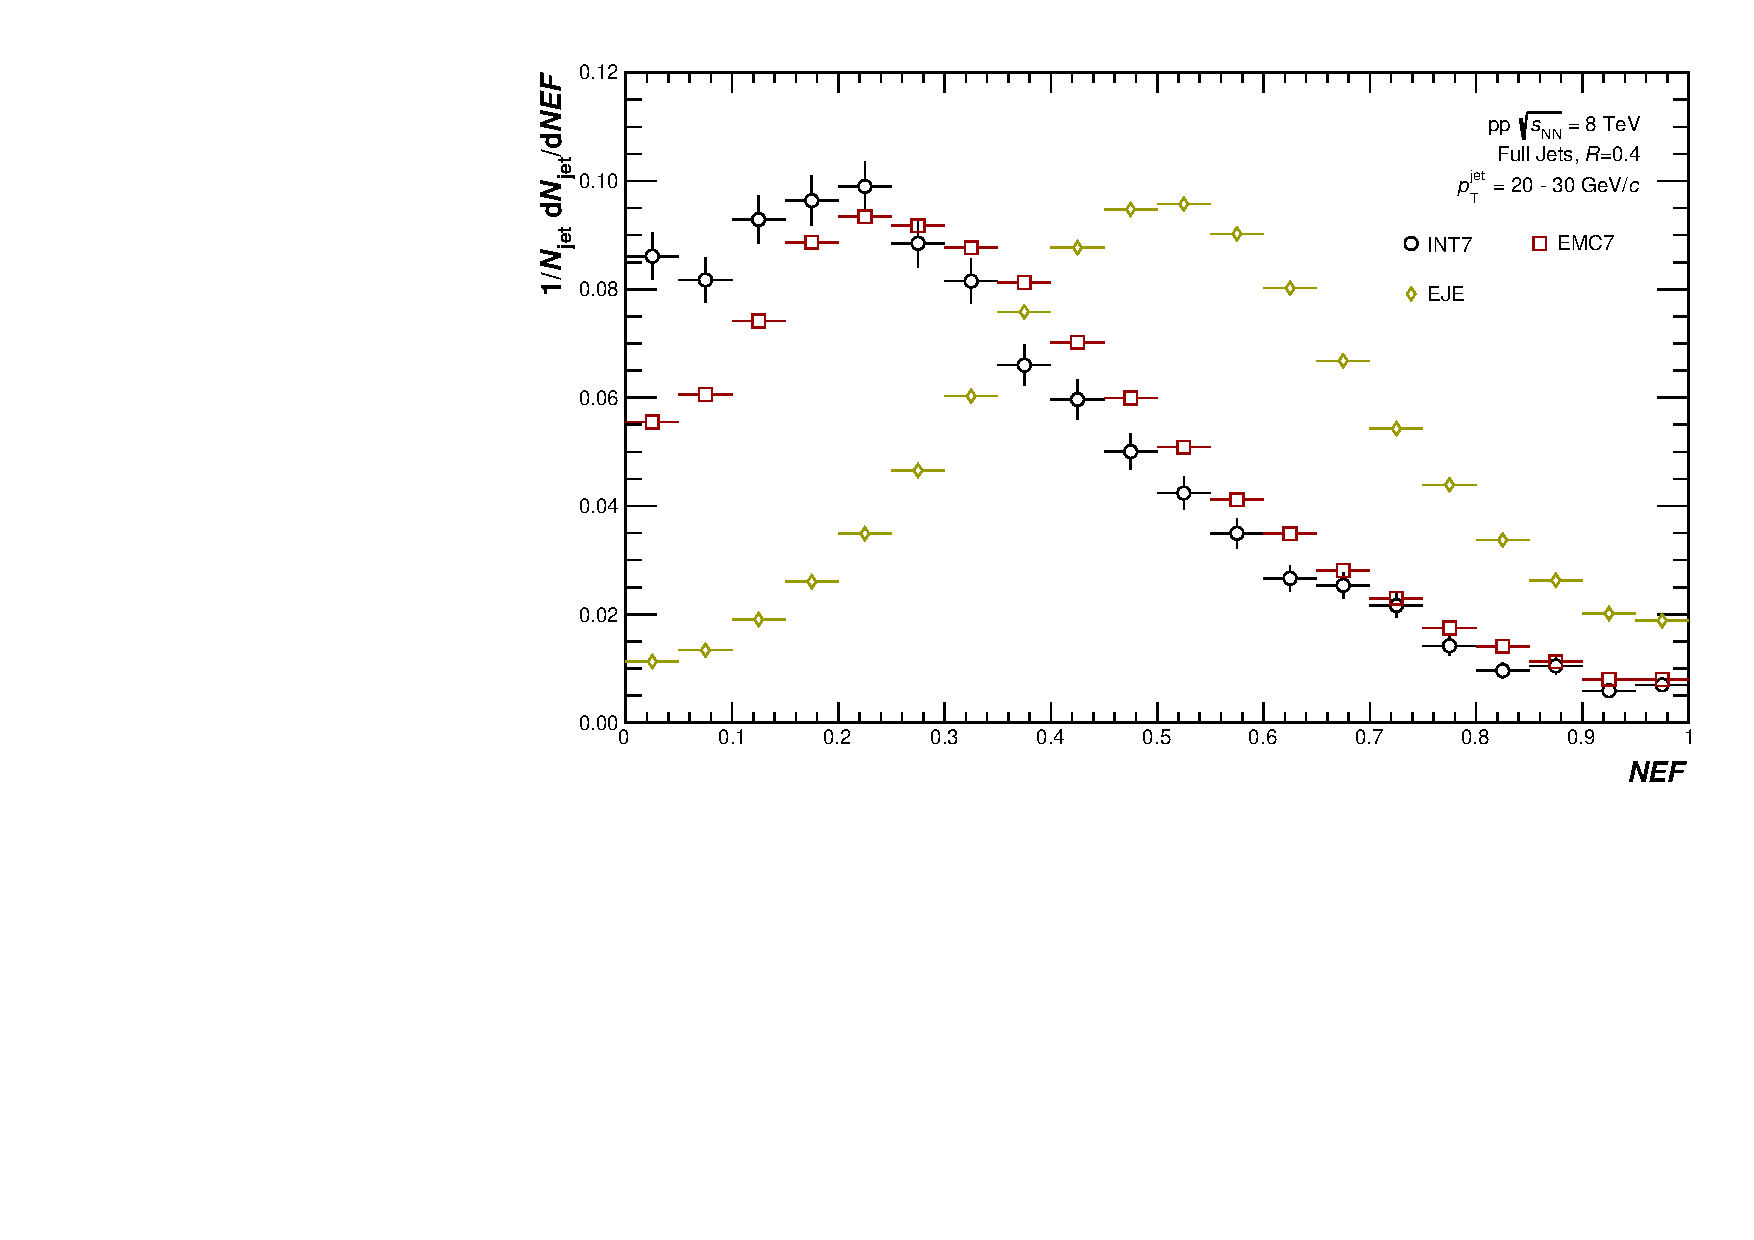
\includegraphics[width=.45\textwidth]{figures/NEF/All/hNEF_20-30GeV_R04.pdf}}
    \qquad
    \subfigure{\label{fig:NEF_30-60GeV_R04}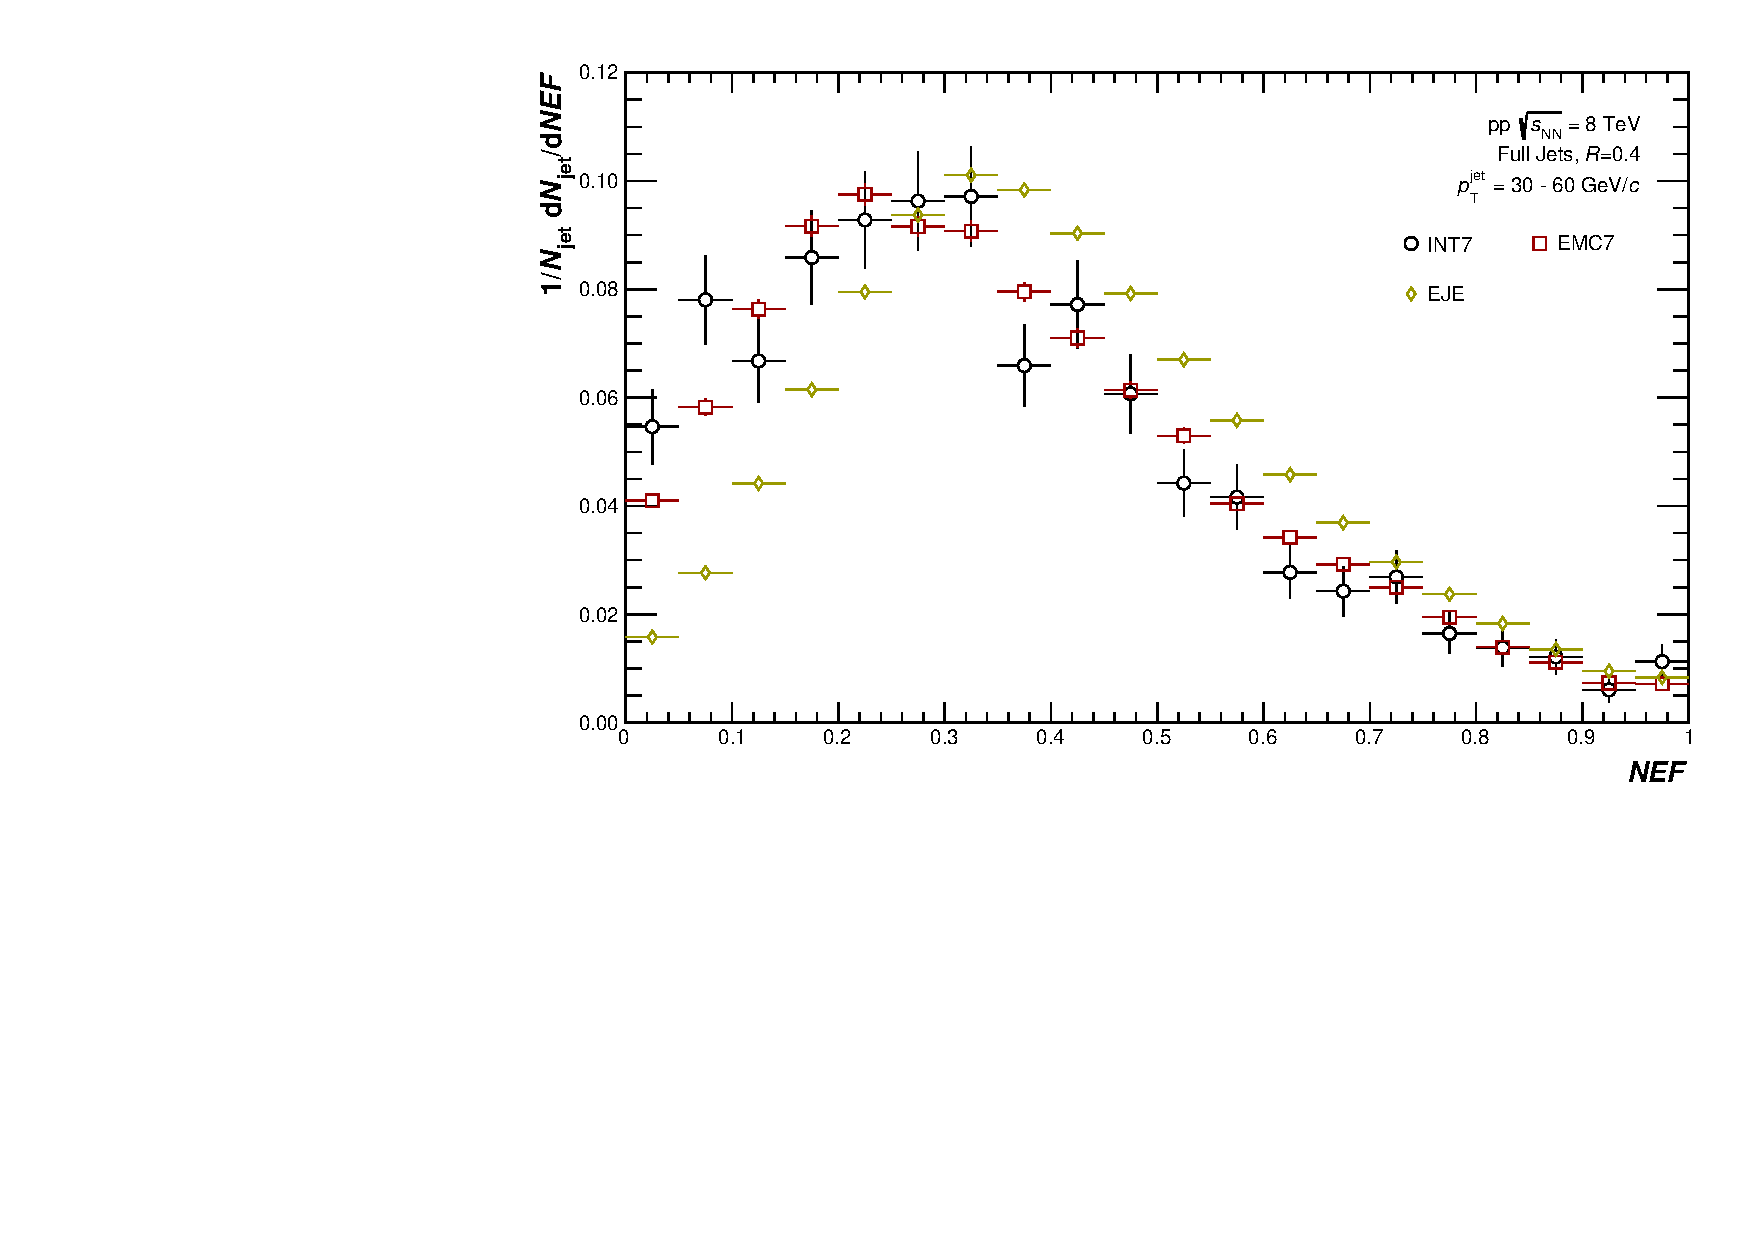
\includegraphics[width=.45\textwidth]{figures/NEF/All/hNEF_30-60GeV_R04.pdf}}\\
    \subfigure{\label{fig:NEF_60-100GeV_R04}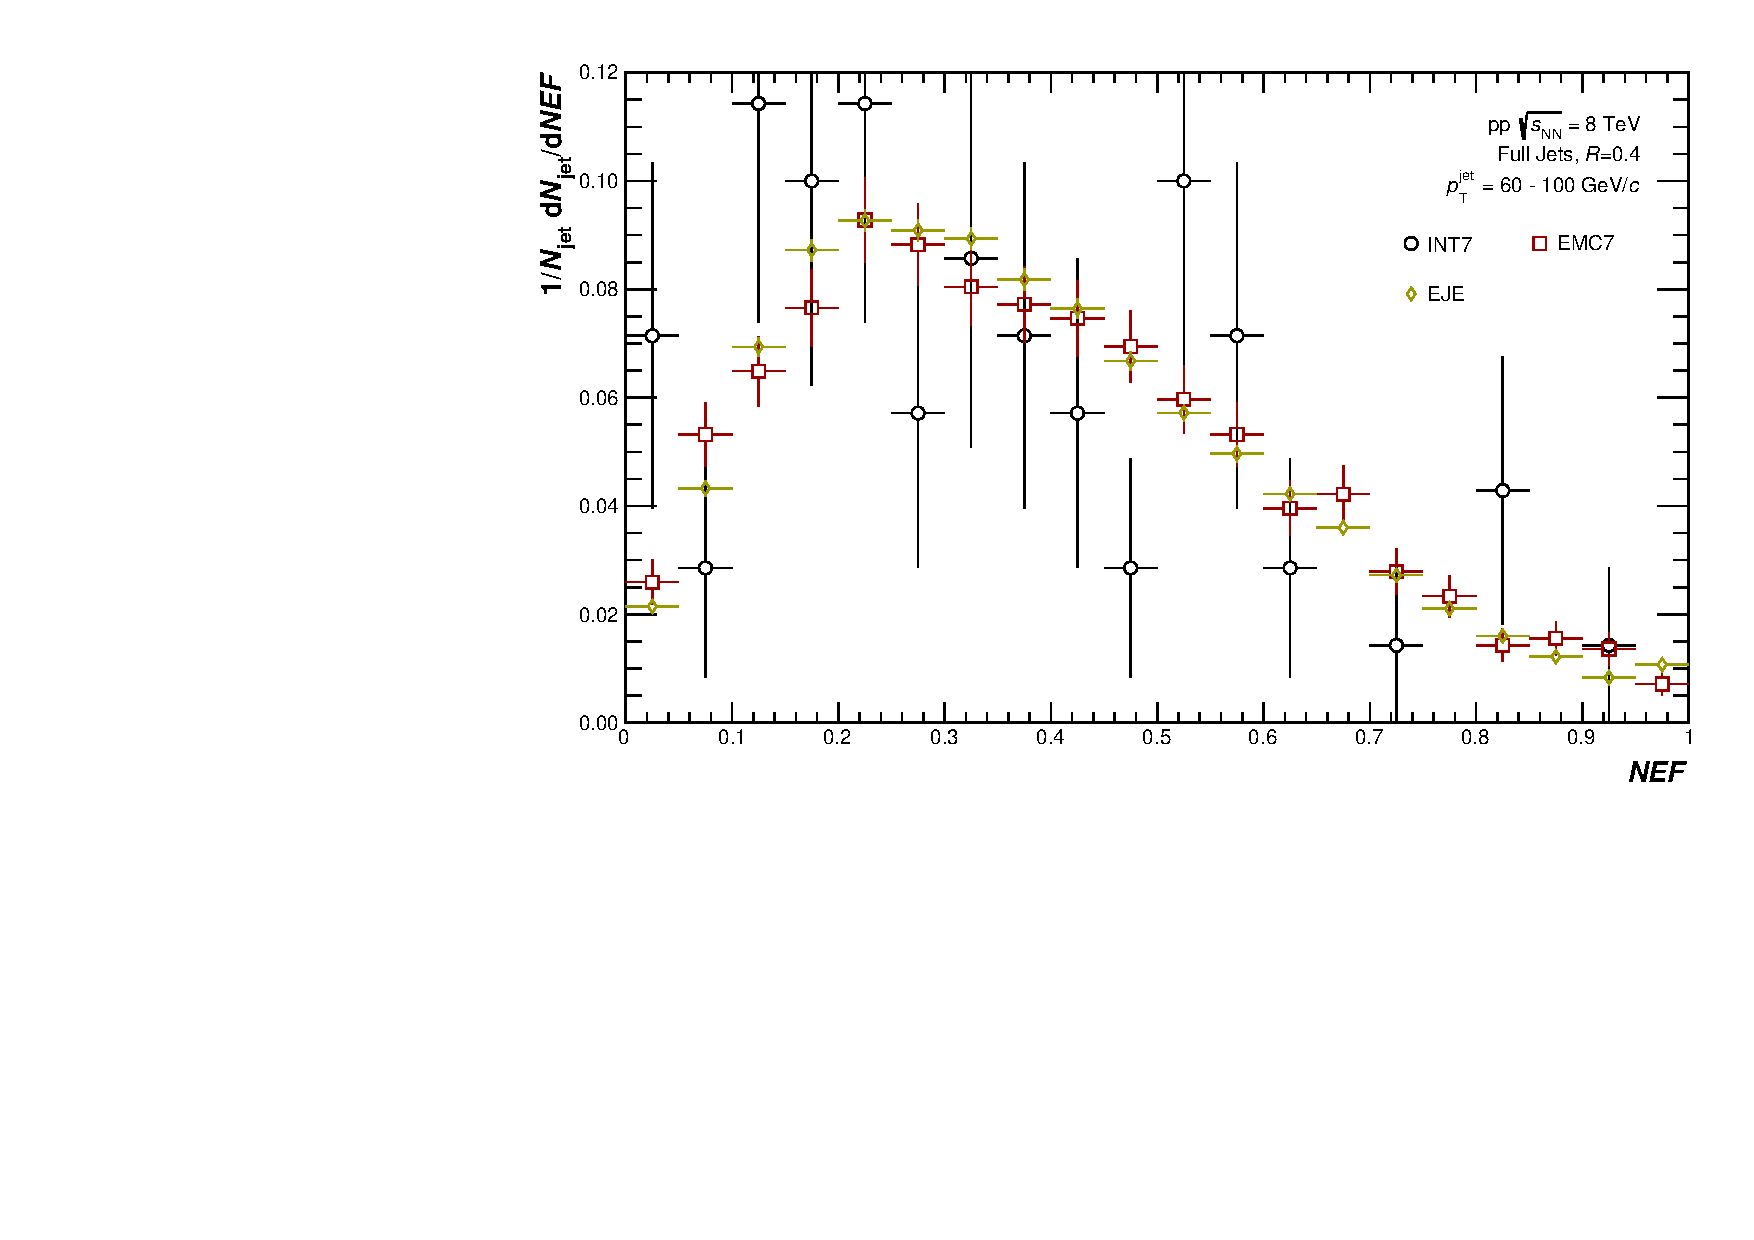
\includegraphics[width=.45\textwidth]{figures/NEF/All/hNEF_60-100GeV_R04.pdf}}
    \qquad
    \subfigure{\label{fig:NEF_100-200GeV_R04}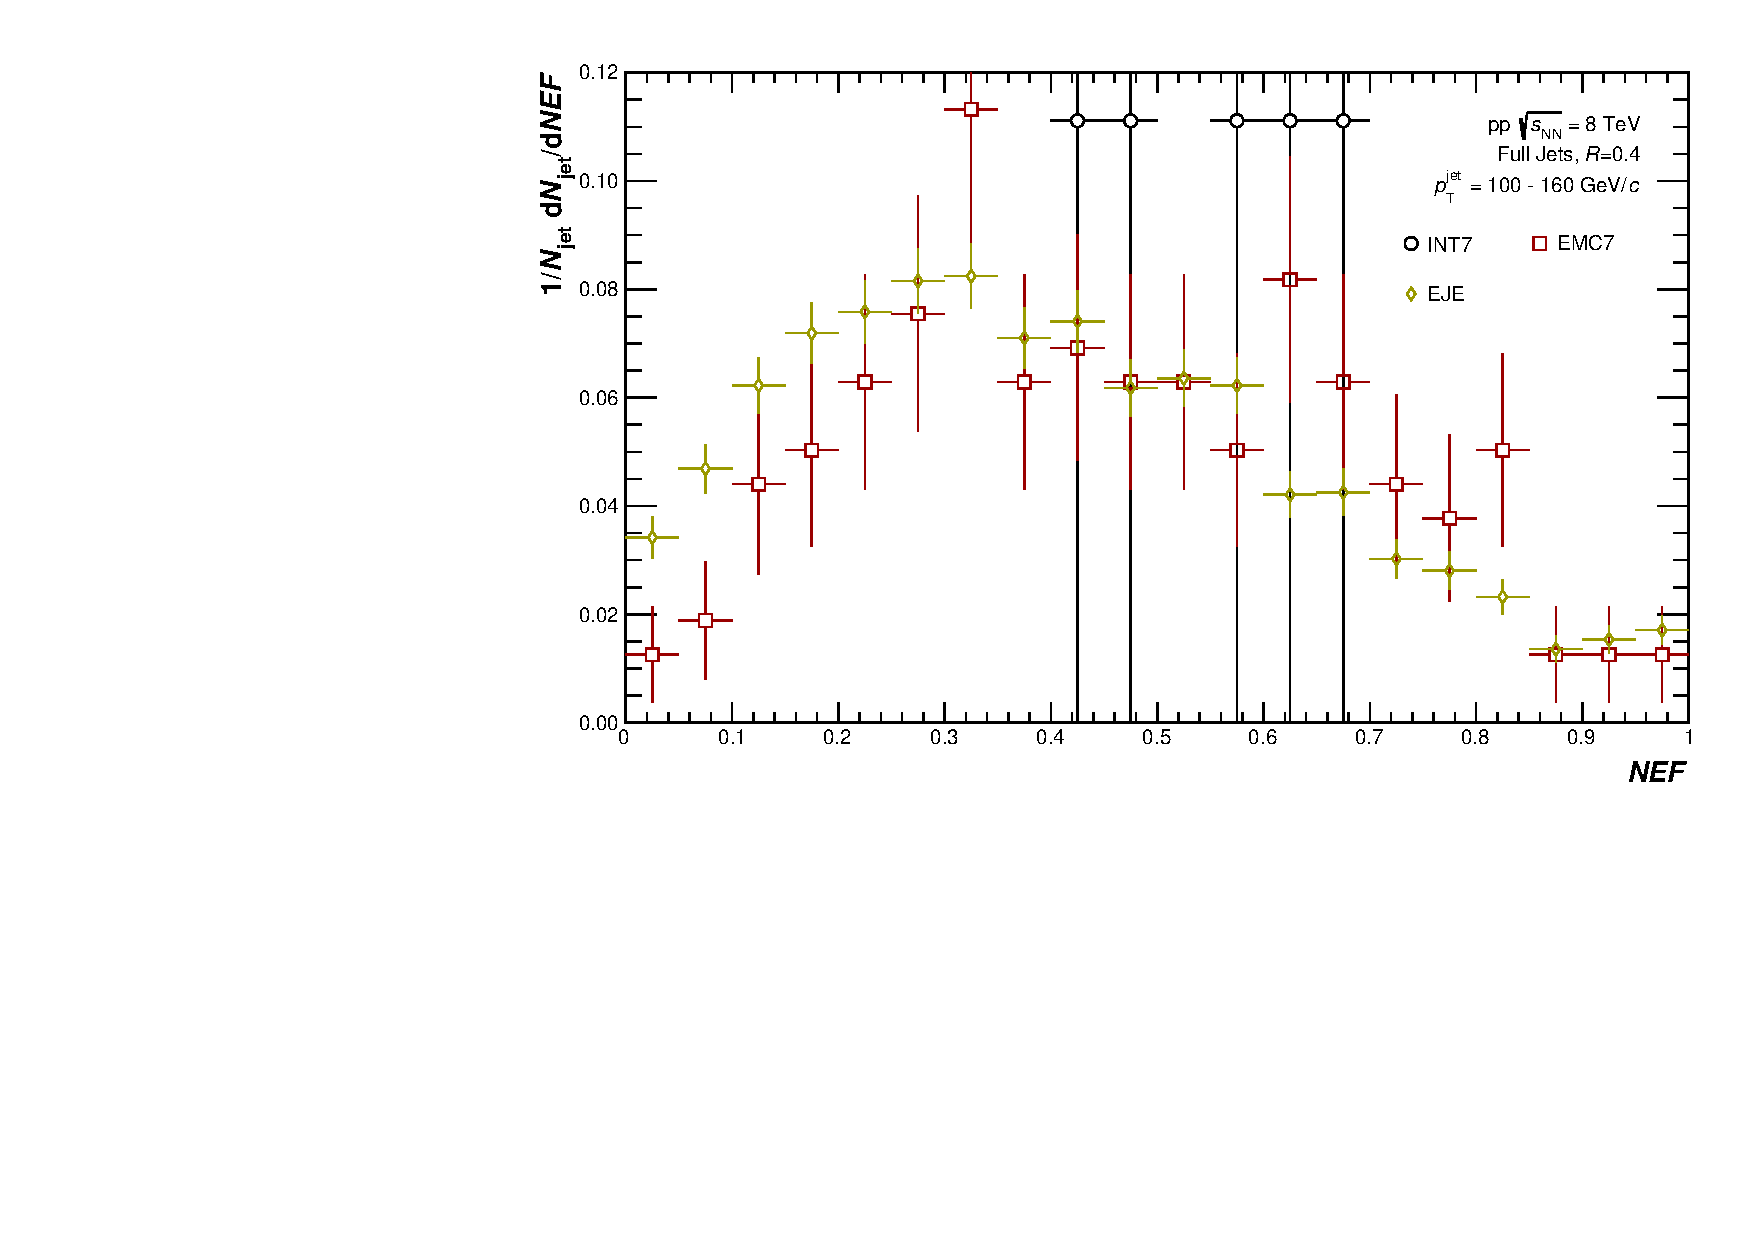
\includegraphics[width=.45\textwidth]{figures/NEF/All/hNEF_100-160GeV_R04.pdf}}\\
    \subfigure{\label{fig:NEF_200-350GeV_R04}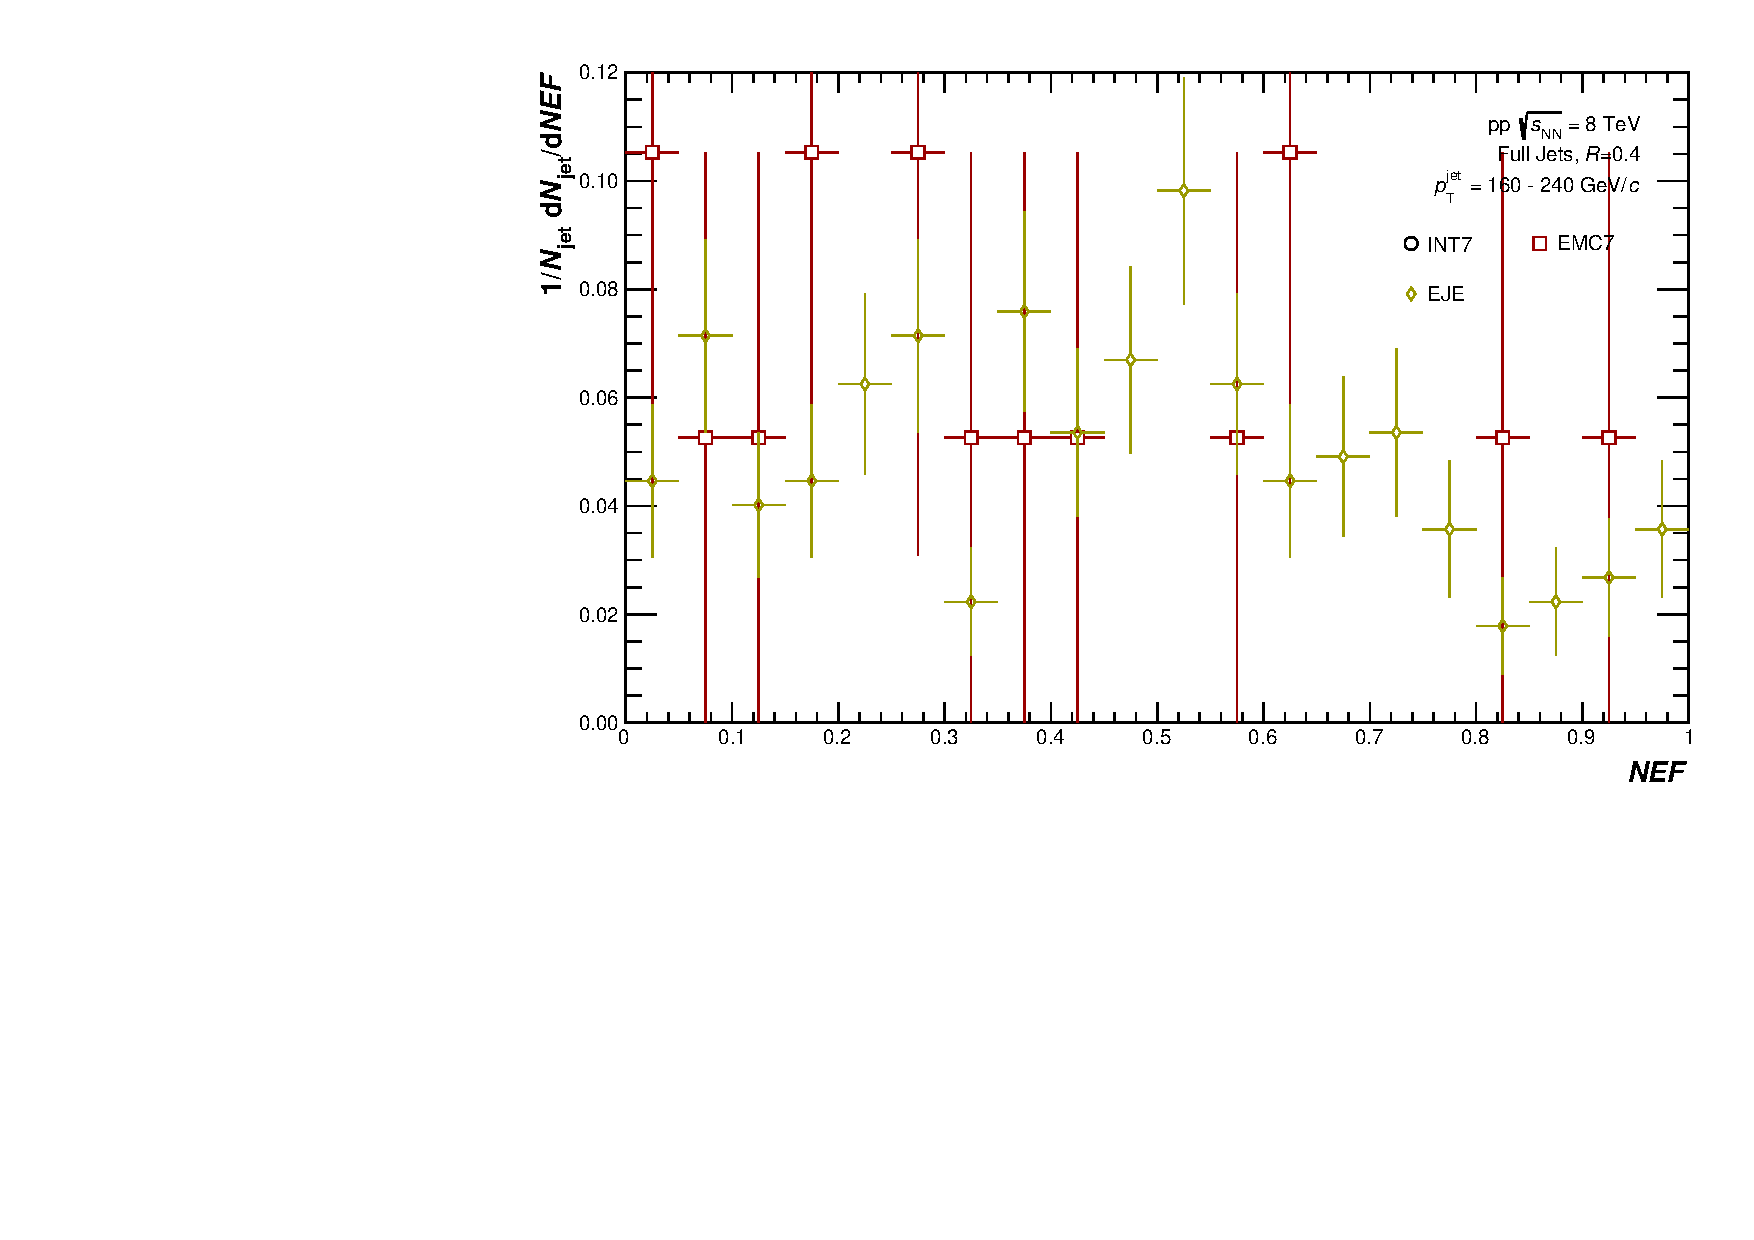
\includegraphics[width=.45\textwidth]{figures/NEF/All/hNEF_160-240GeV_R04.pdf}}
    \caption{NEF for R=0.4 jets in several bins of \pT}
    \label{fig:TriggerBiasNEFR04}
\end{figure}

\newpage

\begin{figure}[h!]
    \centering
    \subfigure{\label{fig:Zch_6-10GeV_R04}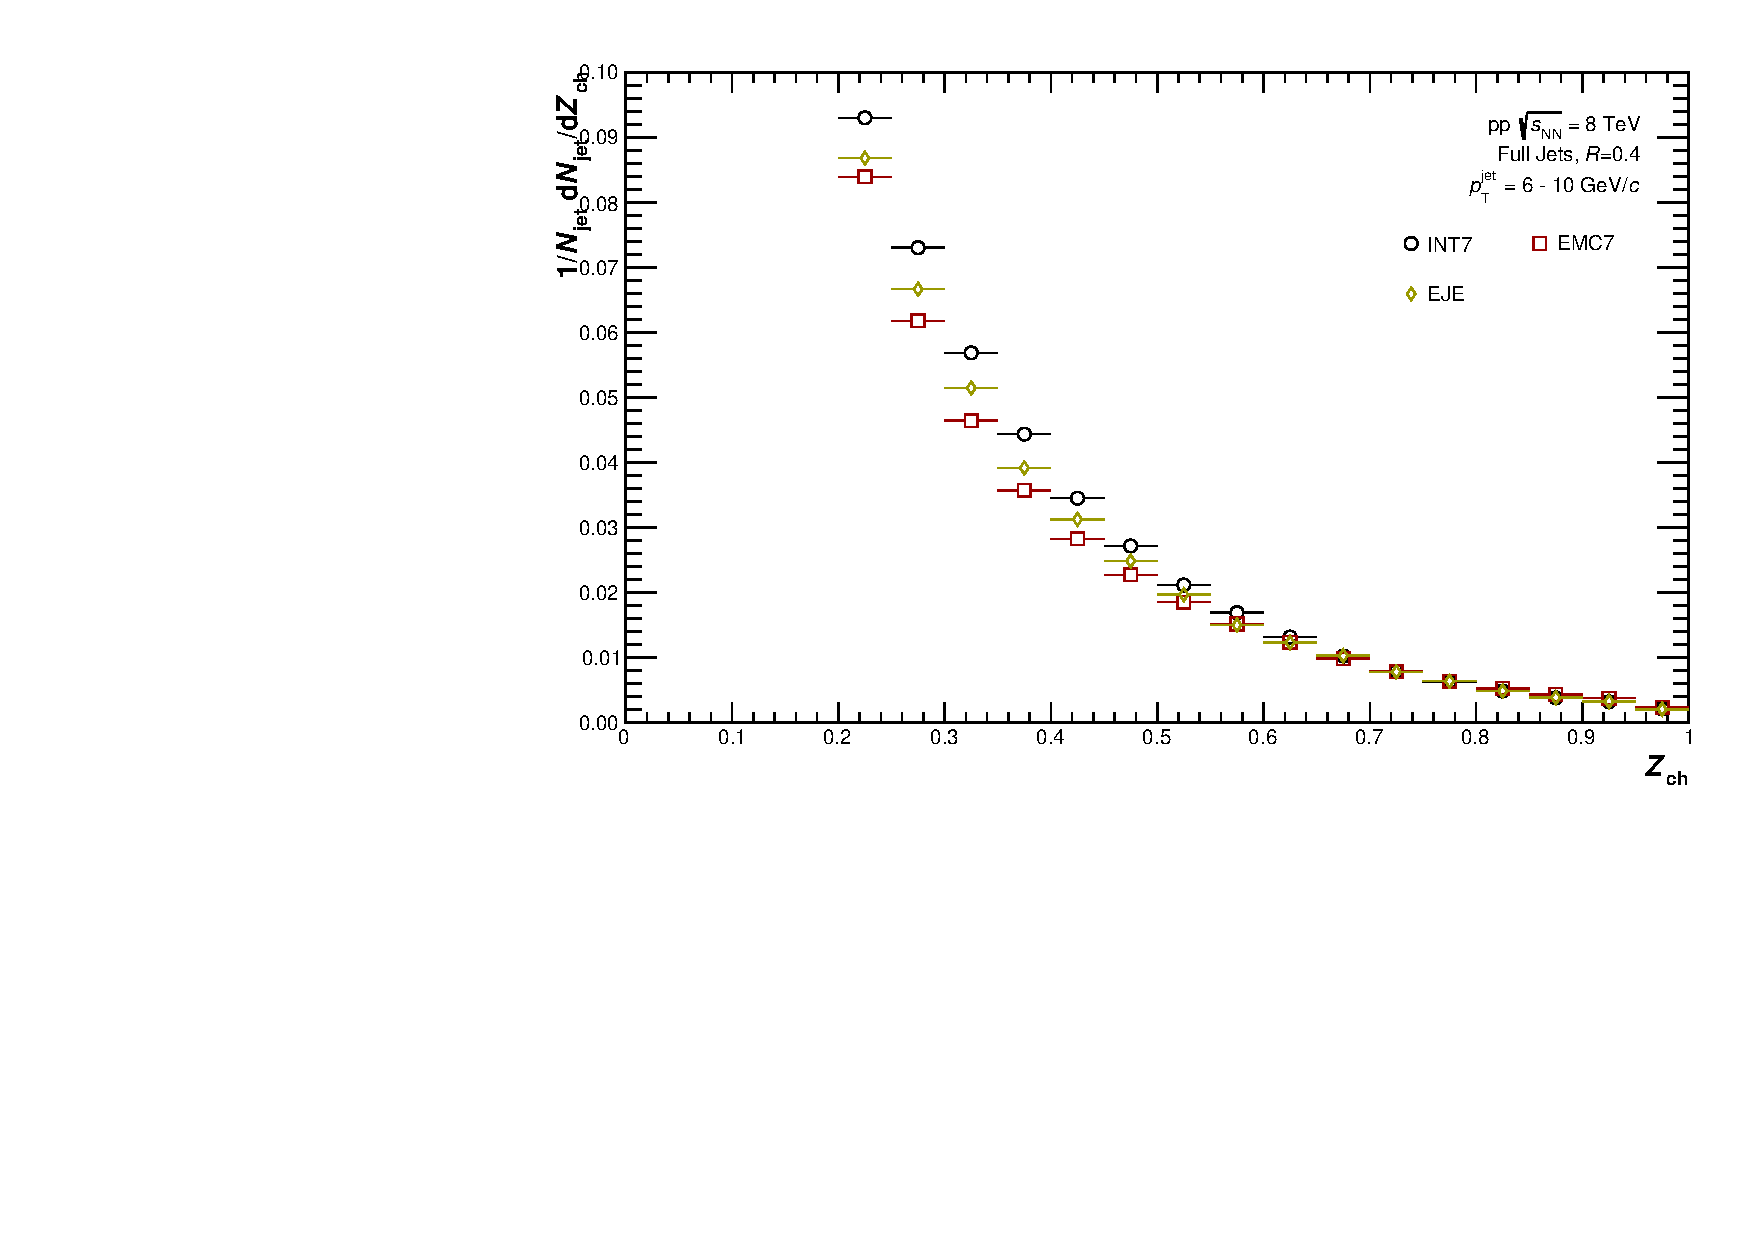
\includegraphics[width=.45\textwidth]{figures/Zch/All/hZch_6-10GeV_R04.pdf}}
    \qquad
    \subfigure{\label{fig:Zch_10-20GeV_R04}\includegraphics[width=.45\textwidth]{figures/Zch/All/hZch_10-20GeV_R04.pdf}}\\
    \subfigure{\label{fig:Zch_20-30GeV_R04}\includegraphics[width=.45\textwidth]{figures/Zch/All/hZch_20-30GeV_R04.pdf}}
    \qquad
    \subfigure{\label{fig:Zch_30-60GeV_R04}\includegraphics[width=.45\textwidth]{figures/Zch/All/hZch_30-60GeV_R04.pdf}}\\
    \subfigure{\label{fig:Zch_60-100GeV_R04}\includegraphics[width=.45\textwidth]{figures/Zch/All/hZch_60-100GeV_R04.pdf}}
    \qquad
    \subfigure{\label{fig:Zch_100-200GeV_R04}\includegraphics[width=.45\textwidth]{figures/Zch/All/hZch_100-160GeV_R04.pdf}}\\
    \subfigure{\label{fig:Zch_200-350GeV_R04}\includegraphics[width=.45\textwidth]{figures/Zch/All/hZch_160-240GeV_R04.pdf}}
    \caption{Z$_{ch}$ for R=0.4 jets in several bins of \pT}
    \label{fig:TriggerBiasZchR04}
\end{figure}

\newpage

\begin{figure}[h!]
    \centering
    \subfigure{\label{fig:Zne_6-10GeV_R04}\includegraphics[width=.45\textwidth]{figures/Zne/All/hZne_6-10GeV_R04.pdf}}
    \qquad
    \subfigure{\label{fig:Zne_10-20GeV_R04}\includegraphics[width=.45\textwidth]{figures/Zne/All/hZne_10-20GeV_R04.pdf}}\\
    \subfigure{\label{fig:Zne_20-30GeV_R04}\includegraphics[width=.45\textwidth]{figures/Zne/All/hZne_20-30GeV_R04.pdf}}
    \qquad
    \subfigure{\label{fig:Zne_30-60GeV_R04}\includegraphics[width=.45\textwidth]{figures/Zne/All/hZne_30-60GeV_R04.pdf}}\\
    \subfigure{\label{fig:Zne_60-100GeV_R04}\includegraphics[width=.45\textwidth]{figures/Zne/All/hZne_60-100GeV_R04.pdf}}
    \qquad
    \subfigure{\label{fig:Zne_100-200GeV_R04}\includegraphics[width=.45\textwidth]{figures/Zne/All/hZne_100-160GeV_R04.pdf}}\\
    \subfigure{\label{fig:Zne_200-350GeV_R04}\includegraphics[width=.45\textwidth]{figures/Zne/All/hZne_160-240GeV_R04.pdf}}
    \caption{Z$_{ne}$ for R=0.4 jets in several bins of \pT}
    \label{fig:TriggerBiasZneR04}
\end{figure}

%%%%%%%%%%%%%%%%%%%%%%%%%%%%%% R=0.5
\newpage

\begin{figure}[h!]
    \centering
    \subfigure{\label{fig:NEF_6-10GeV_R05}\includegraphics[width=.45\textwidth]{figures/NEF/All/hNEF_6-10GeV_R05.pdf}}
    \qquad
    \subfigure{\label{fig:NEF_10-20GeV_R05}\includegraphics[width=.45\textwidth]{figures/NEF/All/hNEF_10-20GeV_R05.pdf}}\\
    \subfigure{\label{fig:NEF_20-30GeV_R05}\includegraphics[width=.45\textwidth]{figures/NEF/All/hNEF_20-30GeV_R05.pdf}}
    \qquad
    \subfigure{\label{fig:NEF_30-60GeV_R05}\includegraphics[width=.45\textwidth]{figures/NEF/All/hNEF_30-60GeV_R05.pdf}}\\
    \subfigure{\label{fig:NEF_60-100GeV_R05}\includegraphics[width=.45\textwidth]{figures/NEF/All/hNEF_60-100GeV_R05.pdf}}
    \qquad
    \subfigure{\label{fig:NEF_100-200GeV_R05}\includegraphics[width=.45\textwidth]{figures/NEF/All/hNEF_100-160GeV_R05.pdf}}\\
    \subfigure{\label{fig:NEF_200-350GeV_R05}\includegraphics[width=.45\textwidth]{figures/NEF/All/hNEF_160-240GeV_R05.pdf}}
    \caption{NEF for R=0.5 jets in several bins of \pT}
    \label{fig:TriggerBiasNEFR05}
\end{figure}

\newpage

\begin{figure}[h!]
    \centering
    \subfigure{\label{fig:Zch_6-10GeV_R05}\includegraphics[width=.45\textwidth]{figures/Zch/All/hZch_6-10GeV_R05.pdf}}
    \qquad
    \subfigure{\label{fig:Zch_10-20GeV_R05}\includegraphics[width=.45\textwidth]{figures/Zch/All/hZch_10-20GeV_R05.pdf}}\\
    \subfigure{\label{fig:Zch_20-30GeV_R05}\includegraphics[width=.45\textwidth]{figures/Zch/All/hZch_20-30GeV_R05.pdf}}
    \qquad
    \subfigure{\label{fig:Zch_30-60GeV_R05}\includegraphics[width=.45\textwidth]{figures/Zch/All/hZch_30-60GeV_R05.pdf}}\\
    \subfigure{\label{fig:Zch_60-100GeV_R05}\includegraphics[width=.45\textwidth]{figures/Zch/All/hZch_60-100GeV_R05.pdf}}
    \qquad
    \subfigure{\label{fig:Zch_100-200GeV_R05}\includegraphics[width=.45\textwidth]{figures/Zch/All/hZch_100-160GeV_R05.pdf}}\\
    \subfigure{\label{fig:Zch_200-350GeV_R05}\includegraphics[width=.45\textwidth]{figures/Zch/All/hZch_160-240GeV_R05.pdf}}
    \caption{Z$_{ch}$ for R=0.5 jets in several bins of \pT}
    \label{fig:TriggerBiasZchR05}
\end{figure}

\newpage

\begin{figure}[h!]
    \centering
    \subfigure{\label{fig:Zne_6-10GeV_R05}\includegraphics[width=.45\textwidth]{figures/Zne/All/hZne_6-10GeV_R05.pdf}}
    \qquad
    \subfigure{\label{fig:Zne_10-20GeV_R05}\includegraphics[width=.45\textwidth]{figures/Zne/All/hZne_10-20GeV_R05.pdf}}\\
    \subfigure{\label{fig:Zne_20-30GeV_R05}\includegraphics[width=.45\textwidth]{figures/Zne/All/hZne_20-30GeV_R05.pdf}}
    \qquad
    \subfigure{\label{fig:Zne_30-60GeV_R05}\includegraphics[width=.45\textwidth]{figures/Zne/All/hZne_30-60GeV_R05.pdf}}\\
    \subfigure{\label{fig:Zne_60-100GeV_R05}\includegraphics[width=.45\textwidth]{figures/Zne/All/hZne_60-100GeV_R05.pdf}}
    \qquad
    \subfigure{\label{fig:Zne_100-200GeV_R05}\includegraphics[width=.45\textwidth]{figures/Zne/All/hZne_100-160GeV_R05.pdf}}\\
    \subfigure{\label{fig:Zne_200-350GeV_R05}\includegraphics[width=.45\textwidth]{figures/Zne/All/hZne_160-240GeV_R05.pdf}}
    \caption{Z$_{ne}$ for R=0.5 jets in several bins of \pT}
    \label{fig:TriggerBiasZneR05}
\end{figure}

%%%%%%%%%%%%%%%%%%%%%%%%%%%%%%%%%%%%%
\newpage

\section{NEF, \texorpdfstring{Z\textsubscript{ch}}{Zch}, and \texorpdfstring{Z\textsubscript{ne}}{Zne} Ratios for Data/MC -- pp}
\label{sec:appendixTriggerBiasRatios}

%%%%%%%%%%%%%%%%%%%%%%%%%%%%%%%%%%%%%%%%%%%%%%%%%% R=02

\begin{figure}[h!]
    \centering
    \subfigure{\includegraphics[width=.45\textwidth]{figures/TriggerBias/NEF/hNEF_ptBin0_R02.pdf}}
    \qquad
    \subfigure{\includegraphics[width=.45\textwidth]{figures/TriggerBias/NEF/hNEF_ptBin2_R02.pdf}}\\
    \subfigure{\includegraphics[width=.45\textwidth]{figures/TriggerBias/NEF/hNEF_ptBin4_R02.pdf}}
    \qquad
    \subfigure{\includegraphics[width=.45\textwidth]{figures/TriggerBias/NEF/hNEF_ptBin1_R02.pdf}}\\
    \subfigure{\includegraphics[width=.45\textwidth]{figures/TriggerBias/NEF/hNEF_ptBin3_R02.pdf}}
    \qquad
    \subfigure{\includegraphics[width=.45\textwidth]{figures/TriggerBias/NEF/hNEF_ptBin5_R02.pdf}}
    \caption{NEF ratios of data to MC for R=0.2.}
    \label{fig:TriggerBiasRatiosNEFR02}
\end{figure}

\newpage

\begin{figure}[h!]
    \centering
    \subfigure{\includegraphics[width=.45\textwidth]{figures/TriggerBias/Zch/hZch_ptBin0_R02.pdf}}
    \qquad
    \subfigure{\includegraphics[width=.45\textwidth]{figures/TriggerBias/Zch/hZch_ptBin2_R02.pdf}}\\
    \subfigure{\includegraphics[width=.45\textwidth]{figures/TriggerBias/Zch/hZch_ptBin4_R02.pdf}}
    \qquad
    \subfigure{\includegraphics[width=.45\textwidth]{figures/TriggerBias/Zch/hZch_ptBin1_R02.pdf}}\\
    \subfigure{\includegraphics[width=.45\textwidth]{figures/TriggerBias/Zch/hZch_ptBin3_R02.pdf}}
    \qquad
    \subfigure{\includegraphics[width=.45\textwidth]{figures/TriggerBias/Zch/hZch_ptBin5_R02.pdf}}
    \caption{Z$_{ch}$ ratios of data to MC for R=0.2.}
    \label{fig:TriggerBiasRatiosZchR02}
\end{figure}

\newpage

\begin{figure}[h!]
    \centering
    \subfigure{\includegraphics[width=.45\textwidth]{figures/TriggerBias/Zne/hZne_ptBin0_R02.pdf}}
    \qquad
    \subfigure{\includegraphics[width=.45\textwidth]{figures/TriggerBias/Zne/hZne_ptBin2_R02.pdf}}\\
    \subfigure{\includegraphics[width=.45\textwidth]{figures/TriggerBias/Zne/hZne_ptBin4_R02.pdf}}
    \qquad
    \subfigure{\includegraphics[width=.45\textwidth]{figures/TriggerBias/Zne/hZne_ptBin1_R02.pdf}}\\
    \subfigure{\includegraphics[width=.45\textwidth]{figures/TriggerBias/Zne/hZne_ptBin3_R02.pdf}}
    \qquad
    \subfigure{\includegraphics[width=.45\textwidth]{figures/TriggerBias/Zne/hZne_ptBin5_R02.pdf}}
    \caption{Z$_{ne}$ ratios of data to MC for R=0.2.}
    \label{fig:TriggerBiasRatiosZneR02}
\end{figure}

%%%%%%%%%%%%%%%%%%%%%%%%%%%%%%%%%%%%%%%% R=0.3
\newpage

\begin{figure}[h!]
    \centering
    \subfigure{\includegraphics[width=.45\textwidth]{figures/TriggerBias/NEF/hNEF_ptBin0_R03.pdf}}
    \qquad
    \subfigure{\includegraphics[width=.45\textwidth]{figures/TriggerBias/NEF/hNEF_ptBin2_R03.pdf}}\\
    \subfigure{\includegraphics[width=.45\textwidth]{figures/TriggerBias/NEF/hNEF_ptBin4_R03.pdf}}
    \qquad
    \subfigure{\includegraphics[width=.45\textwidth]{figures/TriggerBias/NEF/hNEF_ptBin1_R03.pdf}}\\
    \subfigure{\includegraphics[width=.45\textwidth]{figures/TriggerBias/NEF/hNEF_ptBin3_R03.pdf}}
    \qquad
    \subfigure{\includegraphics[width=.45\textwidth]{figures/TriggerBias/NEF/hNEF_ptBin5_R03.pdf}}
    \caption{NEF ratios of data to MC for R=0.3.}
    \label{fig:TriggerBiasRatiosNEFR03}
\end{figure}

\newpage

\begin{figure}[h!]
    \centering
    \subfigure{\includegraphics[width=.45\textwidth]{figures/TriggerBias/Zch/hZch_ptBin0_R03.pdf}}
    \qquad
    \subfigure{\includegraphics[width=.45\textwidth]{figures/TriggerBias/Zch/hZch_ptBin2_R03.pdf}}\\
    \subfigure{\includegraphics[width=.45\textwidth]{figures/TriggerBias/Zch/hZch_ptBin4_R03.pdf}}
    \qquad
    \subfigure{\includegraphics[width=.45\textwidth]{figures/TriggerBias/Zch/hZch_ptBin1_R03.pdf}}\\
    \subfigure{\includegraphics[width=.45\textwidth]{figures/TriggerBias/Zch/hZch_ptBin3_R03.pdf}}
    \qquad
    \subfigure{\includegraphics[width=.45\textwidth]{figures/TriggerBias/Zch/hZch_ptBin5_R03.pdf}}
    \caption{Z$_{ch}$ ratios of data to MC for R=0.3.}
    \label{fig:TriggerBiasRatiosZchR03}
\end{figure}

\newpage

\begin{figure}[h!]
    \centering
    \subfigure{\includegraphics[width=.45\textwidth]{figures/TriggerBias/Zne/hZne_ptBin0_R03.pdf}}
    \qquad
    \subfigure{\includegraphics[width=.45\textwidth]{figures/TriggerBias/Zne/hZne_ptBin2_R03.pdf}}\\
    \subfigure{\includegraphics[width=.45\textwidth]{figures/TriggerBias/Zne/hZne_ptBin4_R03.pdf}}
    \qquad
    \subfigure{\includegraphics[width=.45\textwidth]{figures/TriggerBias/Zne/hZne_ptBin1_R03.pdf}}\\
    \subfigure{\includegraphics[width=.45\textwidth]{figures/TriggerBias/Zne/hZne_ptBin3_R03.pdf}}
    \qquad
    \subfigure{\includegraphics[width=.45\textwidth]{figures/TriggerBias/Zne/hZne_ptBin5_R03.pdf}}
    \caption{Z$_{ne}$ ratios of data to MC for R=0.3.}
    \label{fig:TriggerBiasRatiosZneR03}
\end{figure}

%%%%%%%%%%%%%%%%%%%%%%%%%%%%%%% R=0.4
\newpage

\begin{figure}[h!]
    \centering
    \subfigure{\includegraphics[width=.45\textwidth]{figures/TriggerBias/NEF/hNEF_ptBin0_R04.pdf}}
    \qquad
    \subfigure{\includegraphics[width=.45\textwidth]{figures/TriggerBias/NEF/hNEF_ptBin2_R04.pdf}}\\
    \subfigure{\includegraphics[width=.45\textwidth]{figures/TriggerBias/NEF/hNEF_ptBin4_R04.pdf}}
    \qquad
    \subfigure{\includegraphics[width=.45\textwidth]{figures/TriggerBias/NEF/hNEF_ptBin1_R04.pdf}}\\
    \subfigure{\includegraphics[width=.45\textwidth]{figures/TriggerBias/NEF/hNEF_ptBin3_R04.pdf}}
    \qquad
    \subfigure{\includegraphics[width=.45\textwidth]{figures/TriggerBias/NEF/hNEF_ptBin5_R04.pdf}}
    \caption{NEF ratios of data to MC for R=0.4.}
    \label{fig:TriggerBiasRatiosNEFR04}
\end{figure}

\newpage

\begin{figure}[h!]
    \centering
    \subfigure{\includegraphics[width=.45\textwidth]{figures/TriggerBias/Zch/hZch_ptBin0_R04.pdf}}
    \qquad
    \subfigure{\includegraphics[width=.45\textwidth]{figures/TriggerBias/Zch/hZch_ptBin2_R04.pdf}}\\
    \subfigure{\includegraphics[width=.45\textwidth]{figures/TriggerBias/Zch/hZch_ptBin4_R04.pdf}}
    \qquad
    \subfigure{\includegraphics[width=.45\textwidth]{figures/TriggerBias/Zch/hZch_ptBin1_R04.pdf}}\\
    \subfigure{\includegraphics[width=.45\textwidth]{figures/TriggerBias/Zch/hZch_ptBin3_R04.pdf}}
    \qquad
    \subfigure{\includegraphics[width=.45\textwidth]{figures/TriggerBias/Zch/hZch_ptBin5_R04.pdf}}
    \caption{Z$_{ch}$ ratios of data to MC for R=0.4.}
    \label{fig:TriggerBiasRatiosZchR04}
\end{figure}

\newpage

\begin{figure}[h!]
    \centering
    \subfigure{\includegraphics[width=.45\textwidth]{figures/TriggerBias/Zne/hZne_ptBin0_R04.pdf}}
    \qquad
    \subfigure{\includegraphics[width=.45\textwidth]{figures/TriggerBias/Zne/hZne_ptBin2_R04.pdf}}\\
    \subfigure{\includegraphics[width=.45\textwidth]{figures/TriggerBias/Zne/hZne_ptBin4_R04.pdf}}
    \qquad
    \subfigure{\includegraphics[width=.45\textwidth]{figures/TriggerBias/Zne/hZne_ptBin1_R04.pdf}}\\
    \subfigure{\includegraphics[width=.45\textwidth]{figures/TriggerBias/Zne/hZne_ptBin3_R04.pdf}}
    \qquad
    \subfigure{\includegraphics[width=.45\textwidth]{figures/TriggerBias/Zne/hZne_ptBin5_R04.pdf}}
    \caption{Z$_{ne}$ ratios of data to MC for R=0.4.}
    \label{fig:TriggerBiasRatiosZneR04}
\end{figure}

%%%%%%%%%%%%%%%%%%%%%%%%%%%%%% R=0.5
\newpage

\begin{figure}[h!]
    \centering
    \subfigure{\includegraphics[width=.45\textwidth]{figures/TriggerBias/NEF/hNEF_ptBin0_R05.pdf}}
    \qquad
    \subfigure{\includegraphics[width=.45\textwidth]{figures/TriggerBias/NEF/hNEF_ptBin2_R05.pdf}}\\
    \subfigure{\includegraphics[width=.45\textwidth]{figures/TriggerBias/NEF/hNEF_ptBin4_R05.pdf}}
    \qquad
    \subfigure{\includegraphics[width=.45\textwidth]{figures/TriggerBias/NEF/hNEF_ptBin1_R05.pdf}}\\
    \subfigure{\includegraphics[width=.45\textwidth]{figures/TriggerBias/NEF/hNEF_ptBin3_R05.pdf}}
    \qquad
    \subfigure{\includegraphics[width=.45\textwidth]{figures/TriggerBias/NEF/hNEF_ptBin5_R05.pdf}}
    \caption{NEF ratios of data to MC for R=0.5.}
    \label{fig:TriggerBiasRatiosNEFR05}
\end{figure}

\newpage

\begin{figure}[h!]
    \centering
    \subfigure{\includegraphics[width=.45\textwidth]{figures/TriggerBias/Zch/hZch_ptBin0_R05.pdf}}
    \qquad
    \subfigure{\includegraphics[width=.45\textwidth]{figures/TriggerBias/Zch/hZch_ptBin2_R05.pdf}}\\
    \subfigure{\includegraphics[width=.45\textwidth]{figures/TriggerBias/Zch/hZch_ptBin4_R05.pdf}}
    \qquad
    \subfigure{\includegraphics[width=.45\textwidth]{figures/TriggerBias/Zch/hZch_ptBin1_R05.pdf}}\\
    \subfigure{\includegraphics[width=.45\textwidth]{figures/TriggerBias/Zch/hZch_ptBin3_R05.pdf}}
    \qquad
    \subfigure{\includegraphics[width=.45\textwidth]{figures/TriggerBias/Zch/hZch_ptBin5_R05.pdf}}
    \caption{Z$_{ch}$ ratios of data to MC for R=0.5.}
    \label{fig:TriggerBiasRatiosZchR05}
\end{figure}

\newpage

\begin{figure}[h!]
    \centering
    \subfigure{\includegraphics[width=.45\textwidth]{figures/TriggerBias/Zne/hZne_ptBin0_R05.pdf}}
    \qquad
    \subfigure{\includegraphics[width=.45\textwidth]{figures/TriggerBias/Zne/hZne_ptBin2_R05.pdf}}\\
    \subfigure{\includegraphics[width=.45\textwidth]{figures/TriggerBias/Zne/hZne_ptBin4_R05.pdf}}
    \qquad
    \subfigure{\includegraphics[width=.45\textwidth]{figures/TriggerBias/Zne/hZne_ptBin1_R05.pdf}}\\
    \subfigure{\includegraphics[width=.45\textwidth]{figures/TriggerBias/Zne/hZne_ptBin3_R05.pdf}}
    \qquad
    \subfigure{\includegraphics[width=.45\textwidth]{figures/TriggerBias/Zne/hZne_ptBin5_R05.pdf}}
    \caption{Z$_{ne}$ ratios of data to MC for R=0.5.}
    \label{fig:TriggerBiasRatiosZneR05}
\end{figure}

\section{NEF, \texorpdfstring{Z\textsubscript{ch}}{Zch}, and \texorpdfstring{Z\textsubscript{ne}}{Zne} for Other Radii -- p--Pb}
\label{sec:appendixTriggerBiaspPb}

%%%%%%%%%%%%%%%%%%%%%%%%%%%%%%%%%%%%%%%%%%%%%%%%%% R=02

\begin{figure}[h!]
    \centering
    \subfigure{\label{fig:NEF_6-10GeV_R02pPb}\includegraphics[width=.45\textwidth]{figures/pPbFigures/NEF/All/hNEF_6-10GeV_R02.pdf}}
    \qquad
    \subfigure{\label{fig:NEF_10-20GeV_R02pPb}\includegraphics[width=.45\textwidth]{figures/pPbFigures/NEF/All/hNEF_10-20GeV_R02.pdf}}\\
    \subfigure{\label{fig:NEF_20-30GeV_R02pPb}\includegraphics[width=.45\textwidth]{figures/pPbFigures/NEF/All/hNEF_20-30GeV_R02.pdf}}
    \qquad
    \subfigure{\label{fig:NEF_30-60GeV_R02pPb}\includegraphics[width=.45\textwidth]{figures/pPbFigures/NEF/All/hNEF_30-60GeV_R02.pdf}}\\
    \subfigure{\label{fig:NEF_60-100GeV_R02pPb}\includegraphics[width=.45\textwidth]{figures/pPbFigures/NEF/All/hNEF_60-100GeV_R02.pdf}}
    \qquad
    \subfigure{\label{fig:NEF_100-200GeV_R02pPb}\includegraphics[width=.45\textwidth]{figures/pPbFigures/NEF/All/hNEF_100-160GeV_R02.pdf}}\\
    \subfigure{\label{fig:NEF_200-350GeV_R02pPb}\includegraphics[width=.45\textwidth]{figures/pPbFigures/NEF/All/hNEF_160-240GeV_R02.pdf}}
    \caption{NEF for R=0.2 jets in several bins of \pT}
    \label{fig:appendixTriggerBiasNEFR02pPb}
\end{figure}

\newpage

\begin{figure}[h!]
    \centering
    \subfigure{\label{fig:Zch_6-10GeV_R02pPb}\includegraphics[width=.45\textwidth]{figures/pPbFigures/Zch/All/hZch_6-10GeV_R02.pdf}}
    \qquad
    \subfigure{\label{fig:Zch_10-20GeV_R02pPb}\includegraphics[width=.45\textwidth]{figures/pPbFigures/Zch/All/hZch_10-20GeV_R02.pdf}}\\
    \subfigure{\label{fig:Zch_20-30GeV_R02pPb}\includegraphics[width=.45\textwidth]{figures/pPbFigures/Zch/All/hZch_20-30GeV_R02.pdf}}
    \qquad
    \subfigure{\label{fig:Zch_30-60GeV_R02pPb}\includegraphics[width=.45\textwidth]{figures/pPbFigures/Zch/All/hZch_30-60GeV_R02.pdf}}\\
    \subfigure{\label{fig:Zch_60-100GeV_R02pPb}\includegraphics[width=.45\textwidth]{figures/pPbFigures/Zch/All/hZch_60-100GeV_R02.pdf}}
    \qquad
    \subfigure{\label{fig:Zch_100-200GeV_R02pPb}\includegraphics[width=.45\textwidth]{figures/pPbFigures/Zch/All/hZch_100-160GeV_R02.pdf}}\\
    \subfigure{\label{fig:Zch_200-350GeV_R02pPb}\includegraphics[width=.45\textwidth]{figures/pPbFigures/Zch/All/hZch_160-240GeV_R02.pdf}}
    \caption{Z$_{ch}$ for R=0.2 jets in several bins of \pT}
    \label{fig:TriggerBiasZchR02pPb}
\end{figure}

\newpage

\begin{figure}[h!]
    \centering
    \subfigure{\label{fig:Zne_6-10GeV_R02pPb}\includegraphics[width=.45\textwidth]{figures/pPbFigures/Zne/All/hZne_6-10GeV_R02.pdf}}
    \qquad
    \subfigure{\label{fig:Zne_10-20GeV_R02pPb}\includegraphics[width=.45\textwidth]{figures/pPbFigures/Zne/All/hZne_10-20GeV_R02.pdf}}\\
    \subfigure{\label{fig:Zne_20-30GeV_R02pPb}\includegraphics[width=.45\textwidth]{figures/pPbFigures/Zne/All/hZne_20-30GeV_R02.pdf}}
    \qquad
    \subfigure{\label{fig:Zne_30-60GeV_R02pPb}\includegraphics[width=.45\textwidth]{figures/pPbFigures/Zne/All/hZne_30-60GeV_R02.pdf}}\\
    \subfigure{\label{fig:Zne_60-100GeV_R02pPb}\includegraphics[width=.45\textwidth]{figures/pPbFigures/Zne/All/hZne_60-100GeV_R02.pdf}}
    \qquad
    \subfigure{\label{fig:Zne_100-200GeV_R02pPb}\includegraphics[width=.45\textwidth]{figures/pPbFigures/Zne/All/hZne_100-160GeV_R02.pdf}}\\
    \subfigure{\label{fig:Zne_200-350GeV_R02pPb}\includegraphics[width=.45\textwidth]{figures/pPbFigures/Zne/All/hZne_160-240GeV_R02.pdf}}
    \caption{Z$_{ne}$ for R=0.2 jets in several bins of \pT}
    \label{fig:TriggerBiasZneR02pPb}
\end{figure}

%%%%%%%%%%%%%%%%%%%%%%%%%%%%%%%%%%%%%%%% R=0.3
\newpage

\begin{figure}[h!]
    \centering
    \subfigure{\label{fig:NEF_6-10GeV_R03pPb}\includegraphics[width=.45\textwidth]{figures/pPbFigures/NEF/All/hNEF_6-10GeV_R03.pdf}}
    \qquad
    \subfigure{\label{fig:NEF_10-20GeV_R03pPb}\includegraphics[width=.45\textwidth]{figures/pPbFigures/NEF/All/hNEF_10-20GeV_R03.pdf}}\\
    \subfigure{\label{fig:NEF_20-30GeV_R03pPb}\includegraphics[width=.45\textwidth]{figures/pPbFigures/NEF/All/hNEF_20-30GeV_R03.pdf}}
    \qquad
    \subfigure{\label{fig:NEF_30-60GeV_R03pPb}\includegraphics[width=.45\textwidth]{figures/pPbFigures/NEF/All/hNEF_30-60GeV_R03.pdf}}\\
    \subfigure{\label{fig:NEF_60-100GeV_R03pPb}\includegraphics[width=.45\textwidth]{figures/pPbFigures/NEF/All/hNEF_60-100GeV_R03.pdf}}
    \qquad
    \subfigure{\label{fig:NEF_100-200GeV_R03pPb}\includegraphics[width=.45\textwidth]{figures/pPbFigures/NEF/All/hNEF_100-160GeV_R03.pdf}}\\
    \subfigure{\label{fig:NEF_200-350GeV_R03pPb}\includegraphics[width=.45\textwidth]{figures/pPbFigures/NEF/All/hNEF_160-240GeV_R03.pdf}}
    \caption{NEF for R=0.3 jets in several bins of \pT}
    \label{fig:TriggerBiasNEFR03pPb}
\end{figure}

\newpage

\begin{figure}[h!]
    \centering
    \subfigure{\label{fig:Zch_6-10GeV_R03pPb}\includegraphics[width=.45\textwidth]{figures/pPbFigures/Zch/All/hZch_6-10GeV_R03.pdf}}
    \qquad
    \subfigure{\label{fig:Zch_10-20GeV_R03pPb}\includegraphics[width=.45\textwidth]{figures/pPbFigures/Zch/All/hZch_10-20GeV_R03.pdf}}\\
    \subfigure{\label{fig:Zch_20-30GeV_R03pPb}\includegraphics[width=.45\textwidth]{figures/pPbFigures/Zch/All/hZch_20-30GeV_R03.pdf}}
    \qquad
    \subfigure{\label{fig:Zch_30-60GeV_R03pPb}\includegraphics[width=.45\textwidth]{figures/pPbFigures/Zch/All/hZch_30-60GeV_R03.pdf}}\\
    \subfigure{\label{fig:Zch_60-100GeV_R03pPb}\includegraphics[width=.45\textwidth]{figures/pPbFigures/Zch/All/hZch_60-100GeV_R03.pdf}}
    \qquad
    \subfigure{\label{fig:Zch_100-200GeV_R03pPb}\includegraphics[width=.45\textwidth]{figures/pPbFigures/Zch/All/hZch_100-160GeV_R03.pdf}}\\
    \subfigure{\label{fig:Zch_200-350GeV_R03pPb}\includegraphics[width=.45\textwidth]{figures/pPbFigures/Zch/All/hZch_160-240GeV_R03.pdf}}
    \caption{Z$_{ch}$ for R=0.3 jets in several bins of \pT}
    \label{fig:TriggerBiasZchR03pPb}
\end{figure}

\newpage

\begin{figure}[h!]
    \centering
    \subfigure{\label{fig:Zne_6-10GeV_R03pPb}\includegraphics[width=.45\textwidth]{figures/pPbFigures/Zne/All/hZne_6-10GeV_R03.pdf}}
    \qquad
    \subfigure{\label{fig:Zne_10-20GeV_R03pPb}\includegraphics[width=.45\textwidth]{figures/pPbFigures/Zne/All/hZne_10-20GeV_R03.pdf}}\\
    \subfigure{\label{fig:Zne_20-30GeV_R03pPb}\includegraphics[width=.45\textwidth]{figures/pPbFigures/Zne/All/hZne_20-30GeV_R03.pdf}}
    \qquad
    \subfigure{\label{fig:Zne_30-60GeV_R03pPb}\includegraphics[width=.45\textwidth]{figures/pPbFigures/Zne/All/hZne_30-60GeV_R03.pdf}}\\
    \subfigure{\label{fig:Zne_60-100GeV_R03pPb}\includegraphics[width=.45\textwidth]{figures/pPbFigures/Zne/All/hZne_60-100GeV_R03.pdf}}
    \qquad
    \subfigure{\label{fig:Zne_100-200GeV_R03pPb}\includegraphics[width=.45\textwidth]{figures/pPbFigures/Zne/All/hZne_100-160GeV_R03.pdf}}\\
    \subfigure{\label{fig:Zne_200-350GeV_R03pPb}\includegraphics[width=.45\textwidth]{figures/pPbFigures/Zne/All/hZne_160-240GeV_R03.pdf}}
    \caption{Z$_{ne}$ for R=0.3 jets in several bins of \pT}
    \label{fig:TriggerBiasZneR03pPb}
\end{figure}

%%%%%%%%%%%%%%%%%%%%%%%%%%%%%%% R=0.4
\newpage

\begin{figure}[h!]
    \centering
    \subfigure{\label{fig:NEF_6-10GeV_R04pPb}\includegraphics[width=.45\textwidth]{figures/pPbFigures/NEF/All/hNEF_6-10GeV_R04.pdf}}
    \qquad
    \subfigure{\label{fig:NEF_10-20GeV_R04pPb}\includegraphics[width=.45\textwidth]{figures/pPbFigures/NEF/All/hNEF_10-20GeV_R04.pdf}}\\
    \subfigure{\label{fig:NEF_20-30GeV_R04pPb}\includegraphics[width=.45\textwidth]{figures/pPbFigures/NEF/All/hNEF_20-30GeV_R04.pdf}}
    \qquad
    \subfigure{\label{fig:NEF_30-60GeV_R04pPb}\includegraphics[width=.45\textwidth]{figures/pPbFigures/NEF/All/hNEF_30-60GeV_R04.pdf}}\\
    \subfigure{\label{fig:NEF_60-100GeV_R04pPb}\includegraphics[width=.45\textwidth]{figures/pPbFigures/NEF/All/hNEF_60-100GeV_R04.pdf}}
    \qquad
    \subfigure{\label{fig:NEF_100-200GeV_R04pPb}\includegraphics[width=.45\textwidth]{figures/pPbFigures/NEF/All/hNEF_100-160GeV_R04.pdf}}\\
    \subfigure{\label{fig:NEF_200-350GeV_R04pPb}\includegraphics[width=.45\textwidth]{figures/pPbFigures/NEF/All/hNEF_160-240GeV_R04.pdf}}
    \caption{NEF for R=0.4 jets in several bins of \pT}
    \label{fig:TriggerBiasNEFR04pPb}
\end{figure}

\newpage

\begin{figure}[h!]
    \centering
    \subfigure{\label{fig:Zch_6-10GeV_R04pPb}\includegraphics[width=.45\textwidth]{figures/pPbFigures/Zch/All/hZch_6-10GeV_R04.pdf}}
    \qquad
    \subfigure{\label{fig:Zch_10-20GeV_R04pPb}\includegraphics[width=.45\textwidth]{figures/pPbFigures/Zch/All/hZch_10-20GeV_R04.pdf}}\\
    \subfigure{\label{fig:Zch_20-30GeV_R04pPb}\includegraphics[width=.45\textwidth]{figures/pPbFigures/Zch/All/hZch_20-30GeV_R04.pdf}}
    \qquad
    \subfigure{\label{fig:Zch_30-60GeV_R04pPb}\includegraphics[width=.45\textwidth]{figures/pPbFigures/Zch/All/hZch_30-60GeV_R04.pdf}}\\
    \subfigure{\label{fig:Zch_60-100GeV_R04pPb}\includegraphics[width=.45\textwidth]{figures/pPbFigures/Zch/All/hZch_60-100GeV_R04.pdf}}
    \qquad
    \subfigure{\label{fig:Zch_100-200GeV_R04pPb}\includegraphics[width=.45\textwidth]{figures/pPbFigures/Zch/All/hZch_100-160GeV_R04.pdf}}\\
    \subfigure{\label{fig:Zch_200-350GeV_R04pPb}\includegraphics[width=.45\textwidth]{figures/pPbFigures/Zch/All/hZch_160-240GeV_R04.pdf}}
    \caption{Z$_{ch}$ for R=0.4 jets in several bins of \pT}
    \label{fig:TriggerBiasZchR04pPb}
\end{figure}

\newpage

\begin{figure}[h!]
    \centering
    \subfigure{\label{fig:Zne_6-10GeV_R04pPb}\includegraphics[width=.45\textwidth]{figures/pPbFigures/Zne/All/hZne_6-10GeV_R04.pdf}}
    \qquad
    \subfigure{\label{fig:Zne_10-20GeV_R04pPb}\includegraphics[width=.45\textwidth]{figures/pPbFigures/Zne/All/hZne_10-20GeV_R04.pdf}}\\
    \subfigure{\label{fig:Zne_20-30GeV_R04pPb}\includegraphics[width=.45\textwidth]{figures/pPbFigures/Zne/All/hZne_20-30GeV_R04.pdf}}
    \qquad
    \subfigure{\label{fig:Zne_30-60GeV_R04pPb}\includegraphics[width=.45\textwidth]{figures/pPbFigures/Zne/All/hZne_30-60GeV_R04.pdf}}\\
    \subfigure{\label{fig:Zne_60-100GeV_R04pPb}\includegraphics[width=.45\textwidth]{figures/pPbFigures/Zne/All/hZne_60-100GeV_R04.pdf}}
    \qquad
    \subfigure{\label{fig:Zne_100-200GeV_R04pPb}\includegraphics[width=.45\textwidth]{figures/pPbFigures/Zne/All/hZne_100-160GeV_R04.pdf}}\\
    \subfigure{\label{fig:Zne_200-350GeV_R04pPb}\includegraphics[width=.45\textwidth]{figures/pPbFigures/Zne/All/hZne_160-240GeV_R04.pdf}}
    \caption{Z$_{ne}$ for R=0.4 jets in several bins of \pT}
    \label{fig:TriggerBiasZneR04pPb}
\end{figure}

%%%%%%%%%%%%%%%%%%%%%%%%%%%%%% R=0.5
\newpage

\begin{figure}[h!]
    \centering
    \subfigure{\label{fig:NEF_6-10GeV_R05pPb}\includegraphics[width=.45\textwidth]{figures/pPbFigures/NEF/All/hNEF_6-10GeV_R05.pdf}}
    \qquad
    \subfigure{\label{fig:NEF_10-20GeV_R05pPb}\includegraphics[width=.45\textwidth]{figures/pPbFigures/NEF/All/hNEF_10-20GeV_R05.pdf}}\\
    \subfigure{\label{fig:NEF_20-30GeV_R05pPb}\includegraphics[width=.45\textwidth]{figures/pPbFigures/NEF/All/hNEF_20-30GeV_R05.pdf}}
    \qquad
    \subfigure{\label{fig:NEF_30-60GeV_R05pPb}\includegraphics[width=.45\textwidth]{figures/pPbFigures/NEF/All/hNEF_30-60GeV_R05.pdf}}\\
    \subfigure{\label{fig:NEF_60-100GeV_R05pPb}\includegraphics[width=.45\textwidth]{figures/pPbFigures/NEF/All/hNEF_60-100GeV_R05.pdf}}
    \qquad
    \subfigure{\label{fig:NEF_100-200GeV_R05pPb}\includegraphics[width=.45\textwidth]{figures/pPbFigures/NEF/All/hNEF_100-160GeV_R05.pdf}}\\
    \subfigure{\label{fig:NEF_200-350GeV_R05pPb}\includegraphics[width=.45\textwidth]{figures/pPbFigures/NEF/All/hNEF_160-240GeV_R05.pdf}}
    \caption{NEF for R=0.5 jets in several bins of \pT}
    \label{fig:TriggerBiasNEFR05pPb}
\end{figure}

\newpage

\begin{figure}[h!]
    \centering
    \subfigure{\label{fig:Zch_6-10GeV_R05pPb}\includegraphics[width=.45\textwidth]{figures/pPbFigures/Zch/All/hZch_6-10GeV_R05.pdf}}
    \qquad
    \subfigure{\label{fig:Zch_10-20GeV_R05pPb}\includegraphics[width=.45\textwidth]{figures/pPbFigures/Zch/All/hZch_10-20GeV_R05.pdf}}\\
    \subfigure{\label{fig:Zch_20-30GeV_R05pPb}\includegraphics[width=.45\textwidth]{figures/pPbFigures/Zch/All/hZch_20-30GeV_R05.pdf}}
    \qquad
    \subfigure{\label{fig:Zch_30-60GeV_R05pPb}\includegraphics[width=.45\textwidth]{figures/pPbFigures/Zch/All/hZch_30-60GeV_R05.pdf}}\\
    \subfigure{\label{fig:Zch_60-100GeV_R05pPb}\includegraphics[width=.45\textwidth]{figures/pPbFigures/Zch/All/hZch_60-100GeV_R05.pdf}}
    \qquad
    \subfigure{\label{fig:Zch_100-200GeV_R05pPb}\includegraphics[width=.45\textwidth]{figures/pPbFigures/Zch/All/hZch_100-160GeV_R05.pdf}}\\
    \subfigure{\label{fig:Zch_200-350GeV_R05pPb}\includegraphics[width=.45\textwidth]{figures/pPbFigures/Zch/All/hZch_160-240GeV_R05.pdf}}
    \caption{Z$_{ch}$ for R=0.5 jets in several bins of \pT}
    \label{fig:TriggerBiasZchR05pPb}
\end{figure}

\newpage

\begin{figure}[h!]
    \centering
    \subfigure{\label{fig:Zne_6-10GeV_R05pPb}\includegraphics[width=.45\textwidth]{figures/pPbFigures/Zne/All/hZne_6-10GeV_R05.pdf}}
    \qquad
    \subfigure{\label{fig:Zne_10-20GeV_R05pPb}\includegraphics[width=.45\textwidth]{figures/pPbFigures/Zne/All/hZne_10-20GeV_R05.pdf}}\\
    \subfigure{\label{fig:Zne_20-30GeV_R05pPb}\includegraphics[width=.45\textwidth]{figures/pPbFigures/Zne/All/hZne_20-30GeV_R05.pdf}}
    \qquad
    \subfigure{\label{fig:Zne_30-60GeV_R05pPb}\includegraphics[width=.45\textwidth]{figures/pPbFigures/Zne/All/hZne_30-60GeV_R05.pdf}}\\
    \subfigure{\label{fig:Zne_60-100GeV_R05pPb}\includegraphics[width=.45\textwidth]{figures/pPbFigures/Zne/All/hZne_60-100GeV_R05.pdf}}
    \qquad
    \subfigure{\label{fig:Zne_100-200GeV_R05pPb}\includegraphics[width=.45\textwidth]{figures/pPbFigures/Zne/All/hZne_100-160GeV_R05.pdf}}\\
    \subfigure{\label{fig:Zne_200-350GeV_R05pPb}\includegraphics[width=.45\textwidth]{figures/pPbFigures/Zne/All/hZne_160-240GeV_R05.pdf}}
    \caption{Z$_{ne}$ for R=0.5 jets in several bins of \pT}
    \label{fig:TriggerBiasZneR05pPb}
\end{figure}

%%%%%%%%%%%%%%%%%%%%%%%%%%%%%%%%%%%%%
\newpage

\section{NEF, \texorpdfstring{Z\textsubscript{ch}}{Zch}, and \texorpdfstring{Z\textsubscript{ne}}{Zne} Ratios for Data/MC}
\label{sec:appendixTriggerBiasRatiospPb}

%%%%%%%%%%%%%%%%%%%%%%%%%%%%%%%%%%%%%%%%%%%%%%%%%% R=02

\begin{figure}[h!]
    \centering
    \subfigure{\includegraphics[width=.45\textwidth]{figures/pPbFigures/TriggerBias/NEF/hNEF_ptBin0_R02.pdf}}
    \qquad
    \subfigure{\includegraphics[width=.45\textwidth]{figures/pPbFigures/TriggerBias/NEF/hNEF_ptBin2_R02.pdf}}\\
    \subfigure{\includegraphics[width=.45\textwidth]{figures/pPbFigures/TriggerBias/NEF/hNEF_ptBin4_R02.pdf}}
    \qquad
    \subfigure{\includegraphics[width=.45\textwidth]{figures/pPbFigures/TriggerBias/NEF/hNEF_ptBin1_R02.pdf}}\\
    \subfigure{\includegraphics[width=.45\textwidth]{figures/pPbFigures/TriggerBias/NEF/hNEF_ptBin3_R02.pdf}}
    \qquad
    \subfigure{\includegraphics[width=.45\textwidth]{figures/pPbFigures/TriggerBias/NEF/hNEF_ptBin5_R02.pdf}}
    \caption{NEF ratios of data to MC for R=0.2.}
    \label{fig:TriggerBiasRatiosNEFR02pPb}
\end{figure}

\newpage

\begin{figure}[h!]
    \centering
    \subfigure{\includegraphics[width=.45\textwidth]{figures/pPbFigures/TriggerBias/Zch/hZch_ptBin0_R02.pdf}}
    \qquad
    \subfigure{\includegraphics[width=.45\textwidth]{figures/pPbFigures/TriggerBias/Zch/hZch_ptBin2_R02.pdf}}\\
    \subfigure{\includegraphics[width=.45\textwidth]{figures/pPbFigures/TriggerBias/Zch/hZch_ptBin4_R02.pdf}}
    \qquad
    \subfigure{\includegraphics[width=.45\textwidth]{figures/pPbFigures/TriggerBias/Zch/hZch_ptBin1_R02.pdf}}\\
    \subfigure{\includegraphics[width=.45\textwidth]{figures/pPbFigures/TriggerBias/Zch/hZch_ptBin3_R02.pdf}}
    \qquad
    \subfigure{\includegraphics[width=.45\textwidth]{figures/pPbFigures/TriggerBias/Zch/hZch_ptBin5_R02.pdf}}
    \caption{Z$_{ch}$ ratios of data to MC for R=0.2.}
    \label{fig:TriggerBiasRatiosZchR02pPb}
\end{figure}

\newpage

\begin{figure}[h!]
    \centering
    \subfigure{\includegraphics[width=.45\textwidth]{figures/pPbFigures/TriggerBias/Zne/hZne_ptBin0_R02.pdf}}
    \qquad
    \subfigure{\includegraphics[width=.45\textwidth]{figures/pPbFigures/TriggerBias/Zne/hZne_ptBin2_R02.pdf}}\\
    \subfigure{\includegraphics[width=.45\textwidth]{figures/pPbFigures/TriggerBias/Zne/hZne_ptBin4_R02.pdf}}
    \qquad
    \subfigure{\includegraphics[width=.45\textwidth]{figures/pPbFigures/TriggerBias/Zne/hZne_ptBin1_R02.pdf}}\\
    \subfigure{\includegraphics[width=.45\textwidth]{figures/pPbFigures/TriggerBias/Zne/hZne_ptBin3_R02.pdf}}
    \qquad
    \subfigure{\includegraphics[width=.45\textwidth]{figures/pPbFigures/TriggerBias/Zne/hZne_ptBin5_R02.pdf}}
    \caption{Z$_{ne}$ ratios of data to MC for R=0.2.}
    \label{fig:TriggerBiasRatiosZneR02pPb}
\end{figure}

%%%%%%%%%%%%%%%%%%%%%%%%%%%%%%%%%%%%%%%% R=0.3
\newpage

\begin{figure}[h!]
    \centering
    \subfigure{\includegraphics[width=.45\textwidth]{figures/pPbFigures/TriggerBias/NEF/hNEF_ptBin0_R03.pdf}}
    \qquad
    \subfigure{\includegraphics[width=.45\textwidth]{figures/pPbFigures/TriggerBias/NEF/hNEF_ptBin2_R03.pdf}}\\
    \subfigure{\includegraphics[width=.45\textwidth]{figures/pPbFigures/TriggerBias/NEF/hNEF_ptBin4_R03.pdf}}
    \qquad
    \subfigure{\includegraphics[width=.45\textwidth]{figures/pPbFigures/TriggerBias/NEF/hNEF_ptBin1_R03.pdf}}\\
    \subfigure{\includegraphics[width=.45\textwidth]{figures/pPbFigures/TriggerBias/NEF/hNEF_ptBin3_R03.pdf}}
    \qquad
    \subfigure{\includegraphics[width=.45\textwidth]{figures/pPbFigures/TriggerBias/NEF/hNEF_ptBin5_R03.pdf}}
    \caption{NEF ratios of data to MC for R=0.3.}
    \label{fig:TriggerBiasRatiosNEFR03pPb}
\end{figure}

\newpage

\begin{figure}[h!]
    \centering
    \subfigure{\includegraphics[width=.45\textwidth]{figures/pPbFigures/TriggerBias/Zch/hZch_ptBin0_R03.pdf}}
    \qquad
    \subfigure{\includegraphics[width=.45\textwidth]{figures/pPbFigures/TriggerBias/Zch/hZch_ptBin2_R03.pdf}}\\
    \subfigure{\includegraphics[width=.45\textwidth]{figures/pPbFigures/TriggerBias/Zch/hZch_ptBin4_R03.pdf}}
    \qquad
    \subfigure{\includegraphics[width=.45\textwidth]{figures/pPbFigures/TriggerBias/Zch/hZch_ptBin1_R03.pdf}}\\
    \subfigure{\includegraphics[width=.45\textwidth]{figures/pPbFigures/TriggerBias/Zch/hZch_ptBin3_R03.pdf}}
    \qquad
    \subfigure{\includegraphics[width=.45\textwidth]{figures/pPbFigures/TriggerBias/Zch/hZch_ptBin5_R03.pdf}}
    \caption{Z$_{ch}$ ratios of data to MC for R=0.3.}
    \label{fig:TriggerBiasRatiosZchR03pPb}
\end{figure}

\newpage

\begin{figure}[h!]
    \centering
    \subfigure{\includegraphics[width=.45\textwidth]{figures/pPbFigures/TriggerBias/Zne/hZne_ptBin0_R03.pdf}}
    \qquad
    \subfigure{\includegraphics[width=.45\textwidth]{figures/pPbFigures/TriggerBias/Zne/hZne_ptBin2_R03.pdf}}\\
    \subfigure{\includegraphics[width=.45\textwidth]{figures/pPbFigures/TriggerBias/Zne/hZne_ptBin4_R03.pdf}}
    \qquad
    \subfigure{\includegraphics[width=.45\textwidth]{figures/pPbFigures/TriggerBias/Zne/hZne_ptBin1_R03.pdf}}\\
    \subfigure{\includegraphics[width=.45\textwidth]{figures/pPbFigures/TriggerBias/Zne/hZne_ptBin3_R03.pdf}}
    \qquad
    \subfigure{\includegraphics[width=.45\textwidth]{figures/pPbFigures/TriggerBias/Zne/hZne_ptBin5_R03.pdf}}
    \caption{Z$_{ne}$ ratios of data to MC for R=0.3.}
    \label{fig:TriggerBiasRatiosZneR03pPb}
\end{figure}

%%%%%%%%%%%%%%%%%%%%%%%%%%%%%%% R=0.4
\newpage

\begin{figure}[h!]
    \centering
    \subfigure{\includegraphics[width=.45\textwidth]{figures/pPbFigures/TriggerBias/NEF/hNEF_ptBin0_R04.pdf}}
    \qquad
    \subfigure{\includegraphics[width=.45\textwidth]{figures/pPbFigures/TriggerBias/NEF/hNEF_ptBin2_R04.pdf}}\\
    \subfigure{\includegraphics[width=.45\textwidth]{figures/pPbFigures/TriggerBias/NEF/hNEF_ptBin4_R04.pdf}}
    \qquad
    \subfigure{\includegraphics[width=.45\textwidth]{figures/pPbFigures/TriggerBias/NEF/hNEF_ptBin1_R04.pdf}}\\
    \subfigure{\includegraphics[width=.45\textwidth]{figures/pPbFigures/TriggerBias/NEF/hNEF_ptBin3_R04.pdf}}
    \qquad
    \subfigure{\includegraphics[width=.45\textwidth]{figures/pPbFigures/TriggerBias/NEF/hNEF_ptBin5_R04.pdf}}
    \caption{NEF ratios of data to MC for R=0.4.}
    \label{fig:TriggerBiasRatiosNEFR04pPb}
\end{figure}

\newpage

\begin{figure}[h!]
    \centering
    \subfigure{\includegraphics[width=.45\textwidth]{figures/pPbFigures/TriggerBias/Zch/hZch_ptBin0_R04.pdf}}
    \qquad
    \subfigure{\includegraphics[width=.45\textwidth]{figures/pPbFigures/TriggerBias/Zch/hZch_ptBin2_R04.pdf}}\\
    \subfigure{\includegraphics[width=.45\textwidth]{figures/pPbFigures/TriggerBias/Zch/hZch_ptBin4_R04.pdf}}
    \qquad
    \subfigure{\includegraphics[width=.45\textwidth]{figures/pPbFigures/TriggerBias/Zch/hZch_ptBin1_R04.pdf}}\\
    \subfigure{\includegraphics[width=.45\textwidth]{figures/pPbFigures/TriggerBias/Zch/hZch_ptBin3_R04.pdf}}
    \qquad
    \subfigure{\includegraphics[width=.45\textwidth]{figures/pPbFigures/TriggerBias/Zch/hZch_ptBin5_R04.pdf}}
    \caption{Z$_{ch}$ ratios of data to MC for R=0.4.}
    \label{fig:TriggerBiasRatiosZchR04pPb}
\end{figure}

\newpage

\begin{figure}[h!]
    \centering
    \subfigure{\includegraphics[width=.45\textwidth]{figures/pPbFigures/TriggerBias/Zne/hZne_ptBin0_R04.pdf}}
    \qquad
    \subfigure{\includegraphics[width=.45\textwidth]{figures/pPbFigures/TriggerBias/Zne/hZne_ptBin2_R04.pdf}}\\
    \subfigure{\includegraphics[width=.45\textwidth]{figures/pPbFigures/TriggerBias/Zne/hZne_ptBin4_R04.pdf}}
    \qquad
    \subfigure{\includegraphics[width=.45\textwidth]{figures/pPbFigures/TriggerBias/Zne/hZne_ptBin1_R04.pdf}}\\
    \subfigure{\includegraphics[width=.45\textwidth]{figures/pPbFigures/TriggerBias/Zne/hZne_ptBin3_R04.pdf}}
    \qquad
    \subfigure{\includegraphics[width=.45\textwidth]{figures/pPbFigures/TriggerBias/Zne/hZne_ptBin5_R04.pdf}}
    \caption{Z$_{ne}$ ratios of data to MC for R=0.4.}
    \label{fig:TriggerBiasRatiosZneR04pPb}
\end{figure}

%%%%%%%%%%%%%%%%%%%%%%%%%%%%%% R=0.5
\newpage

\begin{figure}[h!]
    \centering
    \subfigure{\includegraphics[width=.45\textwidth]{figures/pPbFigures/TriggerBias/NEF/hNEF_ptBin0_R05.pdf}}
    \qquad
    \subfigure{\includegraphics[width=.45\textwidth]{figures/pPbFigures/TriggerBias/NEF/hNEF_ptBin2_R05.pdf}}\\
    \subfigure{\includegraphics[width=.45\textwidth]{figures/pPbFigures/TriggerBias/NEF/hNEF_ptBin4_R05.pdf}}
    \qquad
    \subfigure{\includegraphics[width=.45\textwidth]{figures/pPbFigures/TriggerBias/NEF/hNEF_ptBin1_R05.pdf}}\\
    \subfigure{\includegraphics[width=.45\textwidth]{figures/pPbFigures/TriggerBias/NEF/hNEF_ptBin3_R05.pdf}}
    \qquad
    \subfigure{\includegraphics[width=.45\textwidth]{figures/pPbFigures/TriggerBias/NEF/hNEF_ptBin5_R05.pdf}}
    \caption{NEF ratios of data to MC for R=0.5.}
    \label{fig:TriggerBiasRatiosNEFR05pPb}
\end{figure}

\newpage

\begin{figure}[h!]
    \centering
    \subfigure{\includegraphics[width=.45\textwidth]{figures/pPbFigures/TriggerBias/Zch/hZch_ptBin0_R05.pdf}}
    \qquad
    \subfigure{\includegraphics[width=.45\textwidth]{figures/pPbFigures/TriggerBias/Zch/hZch_ptBin2_R05.pdf}}\\
    \subfigure{\includegraphics[width=.45\textwidth]{figures/pPbFigures/TriggerBias/Zch/hZch_ptBin4_R05.pdf}}
    \qquad
    \subfigure{\includegraphics[width=.45\textwidth]{figures/pPbFigures/TriggerBias/Zch/hZch_ptBin1_R05.pdf}}\\
    \subfigure{\includegraphics[width=.45\textwidth]{figures/pPbFigures/TriggerBias/Zch/hZch_ptBin3_R05.pdf}}
    \qquad
    \subfigure{\includegraphics[width=.45\textwidth]{figures/pPbFigures/TriggerBias/Zch/hZch_ptBin5_R05.pdf}}
    \caption{Z$_{ch}$ ratios of data to MC for R=0.5.}
    \label{fig:TriggerBiasRatiosZchR05pPb}
\end{figure}

\newpage

\begin{figure}[h!]
    \centering
    \subfigure{\includegraphics[width=.45\textwidth]{figures/pPbFigures/TriggerBias/Zne/hZne_ptBin0_R05.pdf}}
    \qquad
    \subfigure{\includegraphics[width=.45\textwidth]{figures/pPbFigures/TriggerBias/Zne/hZne_ptBin2_R05.pdf}}\\
    \subfigure{\includegraphics[width=.45\textwidth]{figures/pPbFigures/TriggerBias/Zne/hZne_ptBin4_R05.pdf}}
    \qquad
    \subfigure{\includegraphics[width=.45\textwidth]{figures/pPbFigures/TriggerBias/Zne/hZne_ptBin1_R05.pdf}}\\
    \subfigure{\includegraphics[width=.45\textwidth]{figures/pPbFigures/TriggerBias/Zne/hZne_ptBin3_R05.pdf}}
    \qquad
    \subfigure{\includegraphics[width=.45\textwidth]{figures/pPbFigures/TriggerBias/Zne/hZne_ptBin5_R05.pdf}}
    \caption{Z$_{ne}$ ratios of data to MC for R=0.5.}
    \label{fig:TriggerBiasRatiosZneR05pPb}
\end{figure}

%%%%%%%%%%%%%%%%%%%%%%%%%%%%%%%%%%%%%
\newpage

\section{Jet Energy Scale Slices}
\label{sec:AppendixJES}

Slices of the particle level \pT shift for R = 0.2 jets are shown in Figs. \ref{fig:EnergyScaleSlices1} and \ref{fig:EnergyScaleSlices2}. In the lowest bins, a bias from the jet selection at detector level due to the low \pT cut is visible. The distribution is asymmetric with a tail shifted towards higher \pT. Detector conditions, in particular the fraction of masked or dead area in the EMCal, will have an impact on jet energy scale and resolution. Part of the energy flow of jets overlapping these areas are missing. Small variations between the periods can be observed.

\newpage

\begin{figure}[h!]
    \centering
    \subfigure{\includegraphics[width=.45\textwidth]{figures/EnergyScale/Slices/EnergyScale_R02_10-12GeV.pdf}}
    \qquad
    \subfigure{\includegraphics[width=.45\textwidth]{figures/EnergyScale/Slices/EnergyScale_R02_14-16GeV.pdf}}\\
    \subfigure{\includegraphics[width=.45\textwidth]{figures/EnergyScale/Slices/EnergyScale_R02_20-25GeV.pdf}}
    \qquad
    \subfigure{\includegraphics[width=.45\textwidth]{figures/EnergyScale/Slices/EnergyScale_R02_30-35GeV.pdf}}\\
    \subfigure{\includegraphics[width=.45\textwidth]{figures/EnergyScale/Slices/EnergyScale_R02_12-14GeV.pdf}}
    \qquad
    \subfigure{\includegraphics[width=.45\textwidth]{figures/EnergyScale/Slices/EnergyScale_R02_16-20GeV.pdf}}\\
    \subfigure{\includegraphics[width=.45\textwidth]{figures/EnergyScale/Slices/EnergyScale_R02_25-30GeV.pdf}}
    \qquad
    \subfigure{\includegraphics[width=.45\textwidth]{figures/EnergyScale/Slices/EnergyScale_R02_35-40GeV.pdf}}
    \caption{Distribution of the relative \pT shift between detector and particle level \pT for R = 0.2 jets in different slices in particle level \pT from 10 - 40 GeV/c.}
    \label{fig:EnergyScaleSlices1}
\end{figure}

\newpage

\begin{figure}[h!]
    \centering
    \subfigure{\includegraphics[width=.45\textwidth]{figures/EnergyScale/Slices/EnergyScale_R02_40-50GeV.pdf}}
    \qquad
    \subfigure{\includegraphics[width=.45\textwidth]{figures/EnergyScale/Slices/EnergyScale_R02_60-70GeV.pdf}}\\
    \subfigure{\includegraphics[width=.45\textwidth]{figures/EnergyScale/Slices/EnergyScale_R02_80-100GeV.pdf}}
    \qquad
    \subfigure{\includegraphics[width=.45\textwidth]{figures/EnergyScale/Slices/EnergyScale_R02_120-160GeV.pdf}}\\
    \subfigure{\includegraphics[width=.45\textwidth]{figures/EnergyScale/Slices/EnergyScale_R02_50-60GeV.pdf}}
    \qquad
    \subfigure{\includegraphics[width=.45\textwidth]{figures/EnergyScale/Slices/EnergyScale_R02_70-80GeV.pdf}}\\
    \subfigure{\includegraphics[width=.45\textwidth]{figures/EnergyScale/Slices/EnergyScale_R02_100-120GeV.pdf}}
    \qquad
    \subfigure{\includegraphics[width=.45\textwidth]{figures/EnergyScale/Slices/EnergyScale_R02_160-200GeV.pdf}}
    \caption{Distribution of the relative \pT shift between detector and particle level \pT for R = 0.2 jets in different slices in particle level \pT from 40 - 200 GeV/c.}
    \label{fig:EnergyScaleSlices2}
\end{figure}

%%%%%%%%%%%%%%%%%%%%%%%%%%%%%%%%%%%%%
\newpage

\section{Jet Energy Scale Slices -- p--Pb}
\label{sec:AppendixJESpPb}

Slices of the particle level \pT shift are shown in Figs. \ref{fig:EnergyScaleSlices1pPb} and \ref{fig:EnergyScaleSlices2pPb}. In the lowest bins, a bias from the jet selection at detector level due to the low \pT cut is visible. The distribution is asymmetric with a tail shifted towards higher \pT. Detector conditions, in particular the fraction of masked or dead area in the EMCal, will have an impact on jet energy scale and resolution. Part of the energy flow of jets overlapping these areas are missing. Small variations between the periods can be observed.

\newpage

\begin{figure}[h!]
    \centering
    \subfigure{\includegraphics[width=.45\textwidth]{figures/pPbFigures/EnergyScale/Slices/AllRadii/EnergyScale_AllRadii_10-12GeV.pdf}}
    \qquad
    \subfigure{\includegraphics[width=.45\textwidth]{figures/pPbFigures/EnergyScale/Slices/AllRadii/EnergyScale_AllRadii_14-16GeV.pdf}}\\
    \subfigure{\includegraphics[width=.45\textwidth]{figures/pPbFigures/EnergyScale/Slices/AllRadii/EnergyScale_AllRadii_20-25GeV.pdf}}
    \qquad
    \subfigure{\includegraphics[width=.45\textwidth]{figures/pPbFigures/EnergyScale/Slices/AllRadii/EnergyScale_AllRadii_30-35GeV.pdf}}\\
    \subfigure{\includegraphics[width=.45\textwidth]{figures/pPbFigures/EnergyScale/Slices/AllRadii/EnergyScale_AllRadii_12-14GeV.pdf}}
    \qquad
    \subfigure{\includegraphics[width=.45\textwidth]{figures/pPbFigures/EnergyScale/Slices/AllRadii/EnergyScale_AllRadii_16-20GeV.pdf}}\\
    \subfigure{\includegraphics[width=.45\textwidth]{figures/pPbFigures/EnergyScale/Slices/AllRadii/EnergyScale_AllRadii_25-30GeV.pdf}}
    \qquad
    \subfigure{\includegraphics[width=.45\textwidth]{figures/pPbFigures/EnergyScale/Slices/AllRadii/EnergyScale_AllRadii_35-40GeV.pdf}}
    \caption{Distribution of the relative \pT shift between detector and particle level \pT for R = 0.2 jets in different slices in particle level \pT from 10 - 40 GeV/c.}
    \label{fig:EnergyScaleSlices1pPb}
\end{figure}

\newpage

\begin{figure}[h!]
    \centering
    \subfigure{\includegraphics[width=.45\textwidth]{figures/pPbFigures/EnergyScale/Slices/AllRadii/EnergyScale_AllRadii_40-50GeV.pdf}}
    \qquad
    \subfigure{\includegraphics[width=.45\textwidth]{figures/pPbFigures/EnergyScale/Slices/AllRadii/EnergyScale_AllRadii_60-70GeV.pdf}}\\
    \subfigure{\includegraphics[width=.45\textwidth]{figures/pPbFigures/EnergyScale/Slices/AllRadii/EnergyScale_AllRadii_80-100GeV.pdf}}
    \qquad
    \subfigure{\includegraphics[width=.45\textwidth]{figures/pPbFigures/EnergyScale/Slices/AllRadii/EnergyScale_AllRadii_120-160GeV.pdf}}\\
    \subfigure{\includegraphics[width=.45\textwidth]{figures/pPbFigures/EnergyScale/Slices/AllRadii/EnergyScale_AllRadii_50-60GeV.pdf}}
    \qquad
    \subfigure{\includegraphics[width=.45\textwidth]{figures/pPbFigures/EnergyScale/Slices/AllRadii/EnergyScale_AllRadii_70-80GeV.pdf}}\\
    \subfigure{\includegraphics[width=.45\textwidth]{figures/pPbFigures/EnergyScale/Slices/AllRadii/EnergyScale_AllRadii_100-120GeV.pdf}}
    \qquad
    \subfigure{\includegraphics[width=.45\textwidth]{figures/pPbFigures/EnergyScale/Slices/AllRadii/EnergyScale_AllRadii_160-200GeV.pdf}}
    \caption{Distribution of the relative \pT shift between detector and particle level \pT for R = 0.2 jets in different slices in particle level \pT from 40 - 200 GeV/c.}
    \label{fig:EnergyScaleSlices2pPb}
\end{figure}

\newpage

\section{Individual Systematics Contributions and other jet radii.}
\label{sec:AppendixSystematics}

\subsection{Total Systematics for Other Jet Radii}
\label{subsec:appendixTotalSystematics}

\begin{figure}[h!]
    \centering
    \subfigure{\includegraphics[width=.45\textwidth]{figures/Systematics/TotalSystematics_R03.pdf}}
    \qquad
    \subfigure{\includegraphics[width=.45\textwidth]{figures/Systematics/TotalSystematics_R04.pdf}}\\
    \subfigure{\includegraphics[width=.45\textwidth]{figures/Systematics/TotalSystematics_R05.pdf}}
    \qquad
    \caption{Contribution to the systematic uncertainty for other jet radii.}
    \label{fig:TotalSysOtherR}
\end{figure}

\newpage

\subsection{Individual Contributions}
\label{subsec:appendixIndividualSystematics}

\begin{figure}[h!]
    \centering
    \subfigure{\includegraphics[width=.45\textwidth]{figures/Systematics/R02/clusterizer_bayes_R02_reg6.pdf}}
    \qquad
    \subfigure{\includegraphics[width=.45\textwidth]{figures/Systematics/R02/hadcorr_bayes_R02_reg6.pdf}}\\
    \subfigure{\includegraphics[width=.45\textwidth]{figures/Systematics/R02/allunfolding_bayes_R02_reg6.pdf}}
    \qquad
    \subfigure{\includegraphics[width=.45\textwidth]{figures/Systematics/R02/rffit_bayes_R02_reg6.pdf}}\\
    \subfigure{\includegraphics[width=.45\textwidth]{figures/Systematics/R02/maxclustere_bayes_R02_reg6.pdf}}
    \caption{Individual contributions to the systematic uncertainty for R=0.2, page 1.}
    \label{fig:IndividualSysR02_1}
\end{figure}
\newpage

\begin{figure}[h!]
    \centering
    \subfigure{\includegraphics[width=.45\textwidth]{figures/Systematics/R02/seedcell_bayes_R02_reg6.pdf}}
    \qquad
    \subfigure{\includegraphics[width=.45\textwidth]{figures/Systematics/R02/trackeff_bayes_R02_reg6.pdf}}\\
    \subfigure{\includegraphics[width=.45\textwidth]{figures/Systematics/R02/triggerswap_bayes_R02_reg6.pdf}}
    \qquad
    \subfigure{\includegraphics[width=.45\textwidth]{figures/Systematics/R02/maxtrackpt_bayes_R02_reg6.pdf}}
    \caption{Individual contributions to the systematic uncertainty for R=0.2, page 2.}
    \label{fig:IndividualSysR02_2}
\end{figure}

\newpage

\begin{figure}[h!]
    \centering
    \subfigure{\includegraphics[width=.45\textwidth]{figures/Systematics/R03/clusterizer_bayes_R03_reg6.pdf}}
    \qquad
    \subfigure{\includegraphics[width=.45\textwidth]{figures/Systematics/R03/hadcorr_bayes_R03_reg6.pdf}}\\
    \subfigure{\includegraphics[width=.45\textwidth]{figures/Systematics/R03/allunfolding_bayes_R03_reg6.pdf}}
    \qquad
    \subfigure{\includegraphics[width=.45\textwidth]{figures/Systematics/R03/maxclustere_bayes_R03_reg6.pdf}}\\
    \subfigure{\includegraphics[width=.45\textwidth]{figures/Systematics/R03/seedcell_bayes_R03_reg6.pdf}}
    \qquad
    \subfigure{\includegraphics[width=.45\textwidth]{figures/Systematics/R03/trackeff_bayes_R03_reg6.pdf}}\\
    \subfigure{\includegraphics[width=.45\textwidth]{figures/Systematics/R03/triggerswap_bayes_R03_reg6.pdf}}
    \qquad
    \subfigure{\includegraphics[width=.45\textwidth]{figures/Systematics/R03/maxtrackpt_bayes_R03_reg6.pdf}}
    \caption{Individual contributions to the systematic uncertainty for R=0.3.}
    \label{fig:IndividualSysR03}
\end{figure}

\newpage

\begin{figure}[h!]
    \centering
    \subfigure{\includegraphics[width=.45\textwidth]{figures/Systematics/R04/clusterizer_bayes_R04_reg6.pdf}}
    \qquad
    \subfigure{\includegraphics[width=.45\textwidth]{figures/Systematics/R04/hadcorr_bayes_R04_reg6.pdf}}\\
    \subfigure{\includegraphics[width=.45\textwidth]{figures/Systematics/R04/allunfolding_bayes_R04_reg6.pdf}}
    \qquad
    \subfigure{\includegraphics[width=.45\textwidth]{figures/Systematics/R04/maxclustere_bayes_R04_reg6.pdf}}\\
    \subfigure{\includegraphics[width=.45\textwidth]{figures/Systematics/R04/seedcell_bayes_R04_reg6.pdf}}
    \qquad
    \subfigure{\includegraphics[width=.45\textwidth]{figures/Systematics/R04/trackeff_bayes_R04_reg6.pdf}}\\
    \subfigure{\includegraphics[width=.45\textwidth]{figures/Systematics/R04/triggerswap_bayes_R04_reg6.pdf}}
    \qquad
    \subfigure{\includegraphics[width=.45\textwidth]{figures/Systematics/R04/maxtrackpt_bayes_R04_reg6.pdf}}
    \caption{Individual contributions to the systematic uncertainty for R=0.4.}
    \label{fig:IndividualSysR04}
\end{figure}

\newpage

\begin{figure}[h!]
    \centering
    \subfigure{\includegraphics[width=.45\textwidth]{figures/Systematics/R05/clusterizer_bayes_R05_reg6.pdf}}
    \qquad
    \subfigure{\includegraphics[width=.45\textwidth]{figures/Systematics/R05/hadcorr_bayes_R05_reg6.pdf}}\\
    \subfigure{\includegraphics[width=.45\textwidth]{figures/Systematics/R05/allunfolding_bayes_R05_reg6.pdf}}
    \qquad
    \subfigure{\includegraphics[width=.45\textwidth]{figures/Systematics/R05/maxclustere_bayes_R05_reg6.pdf}}\\
    \subfigure{\includegraphics[width=.45\textwidth]{figures/Systematics/R05/seedcell_bayes_R05_reg6.pdf}}
    \qquad
    \subfigure{\includegraphics[width=.45\textwidth]{figures/Systematics/R05/trackeff_bayes_R05_reg6.pdf}}\\
    \subfigure{\includegraphics[width=.45\textwidth]{figures/Systematics/R05/triggerswap_bayes_R05_reg6.pdf}}
    \qquad
    \subfigure{\includegraphics[width=.45\textwidth]{figures/Systematics/R05/maxtrackpt_bayes_R05_reg6.pdf}}
    \caption{Individual contributions to the systematic uncertainty for R=0.5.}
    \label{fig:IndividualSysR05}
\end{figure}

\newpage

\section{Individual Systematics Contributions for Ratios and Ratios of Other Radii}
\label{sec:AppendixSystematicsRatios}

\subsection{Total Systematics for Other Ratios}
\label{subsec:appendixTotalSystematicsRatios}

\begin{figure}[h!]
    \centering
    \subfigure{\includegraphics[width=.45\textwidth]{figures/Systematics/ratios/TotalSystematics_R02R03.pdf}}
    \qquad
    \subfigure{\includegraphics[width=.45\textwidth]{figures/Systematics/ratios/TotalSystematics_R02R04.pdf}}\\
    \subfigure{\includegraphics[width=.45\textwidth]{figures/Systematics/ratios/TotalSystematics_R02R05.pdf}}
    \qquad
    \caption{Contribution to the systematic uncertainty for other ratios.}
    \label{fig:TotalSysRatiosOtherR}
\end{figure}

\newpage

\subsection{Individual Contributions}
\label{subsec:appendixIndividualSystematicsRatios}

\begin{figure}[h!]
    \centering
    \subfigure{\includegraphics[width=.45\textwidth]{figures/Systematics/ratios/R02R03/clusterizer_bayes_R02R03_reg6.pdf}}
    \qquad
    \subfigure{\includegraphics[width=.45\textwidth]{figures/Systematics/ratios/R02R03/hadcorr_bayes_R02R03_reg6.pdf}}\\
    \qquad
    \subfigure{\includegraphics[width=.45\textwidth]{figures/Systematics/ratios/R02R03/maxclustere_bayes_R02R03_reg6.pdf}}\\
    \subfigure{\includegraphics[width=.45\textwidth]{figures/Systematics/ratios/R02R03/seedcell_bayes_R02R03_reg6.pdf}}
    \qquad
    \subfigure{\includegraphics[width=.45\textwidth]{figures/Systematics/ratios/R02R03/trackeff_bayes_R02R03_reg6.pdf}}\\
    \qquad
    \subfigure{\includegraphics[width=.45\textwidth]{figures/Systematics/ratios/R02R03/maxtrackpt_bayes_R02R03_reg6.pdf}}
    \caption{Individual contributions to the systematic uncertainty for R=0.2/0.3.}
    \label{fig:IndividualSysRatiosR03}
\end{figure}

\newpage

\begin{figure}[h!]
    \centering
    \subfigure{\includegraphics[width=.45\textwidth]{figures/Systematics/ratios/R02R04/clusterizer_bayes_R02R04_reg6.pdf}}
    \qquad
    \subfigure{\includegraphics[width=.45\textwidth]{figures/Systematics/ratios/R02R04/hadcorr_bayes_R02R04_reg6.pdf}}\\
    \qquad
    \subfigure{\includegraphics[width=.45\textwidth]{figures/Systematics/ratios/R02R04/maxclustere_bayes_R02R04_reg6.pdf}}\\
    \subfigure{\includegraphics[width=.45\textwidth]{figures/Systematics/ratios/R02R04/seedcell_bayes_R02R04_reg6.pdf}}
    \qquad
    \subfigure{\includegraphics[width=.45\textwidth]{figures/Systematics/ratios/R02R04/trackeff_bayes_R02R04_reg6.pdf}}\\
    \qquad
    \subfigure{\includegraphics[width=.45\textwidth]{figures/Systematics/ratios/R02R04/maxtrackpt_bayes_R02R04_reg6.pdf}}
    \caption{Individual contributions to the systematic uncertainty for R=0.2/0.4.}
    \label{fig:IndividualSysRatiosR04}
\end{figure}

\newpage

\begin{figure}[h!]
    \centering
    \subfigure{\includegraphics[width=.45\textwidth]{figures/Systematics/ratios/R02R05/clusterizer_bayes_R02R05_reg6.pdf}}
    \qquad
    \subfigure{\includegraphics[width=.45\textwidth]{figures/Systematics/ratios/R02R05/hadcorr_bayes_R02R05_reg6.pdf}}\\
    \qquad
    \subfigure{\includegraphics[width=.45\textwidth]{figures/Systematics/ratios/R02R05/maxclustere_bayes_R02R05_reg6.pdf}}\\
    \subfigure{\includegraphics[width=.45\textwidth]{figures/Systematics/ratios/R02R05/seedcell_bayes_R02R05_reg6.pdf}}
    \qquad
    \subfigure{\includegraphics[width=.45\textwidth]{figures/Systematics/ratios/R02R05/trackeff_bayes_R02R05_reg6.pdf}}\\
    \qquad
    \subfigure{\includegraphics[width=.45\textwidth]{figures/Systematics/ratios/R02R05/maxtrackpt_bayes_R02R05_reg6.pdf}}
    \caption{Individual contributions to the systematic uncertainty for R=0.2/0.5.}
    \label{fig:IndividualSysRatiosR05}
\end{figure}

\newpage

\section{Individual Systematics Contributions and other jet radii. -- p--Pb}
\label{sec:AppendixSystematicspPb}

\subsection{Total Systematics for Other Jet Radii -- p--Pb}
\label{subsec:appendixTotalSystematicspPb}

\begin{figure}[h!]
    \centering
    \subfigure{\includegraphics[width=.45\textwidth]{figures/pPbFigures/Systematics/TotalSystematics_R03.pdf}}
    \qquad
    \subfigure{\includegraphics[width=.45\textwidth]{figures/pPbFigures/Systematics/TotalSystematics_R04.pdf}}\\
    \caption{Contribution to the systematic uncertainty for other jet radii.}
    \label{fig:TotalSysOtherRpPb}
\end{figure}

\newpage

\subsection{Individual Contributions}
\label{subsec:appendixIndividualSystematicspPb}

\begin{figure}[h!]
    \centering
    \subfigure{\includegraphics[width=.45\textwidth]{figures/pPbFigures/Systematics/R02/clusterizer_bayes_R02_reg6.pdf}}
    \qquad
    \subfigure{\includegraphics[width=.45\textwidth]{figures/pPbFigures/Systematics/R02/hadcorr_bayes_R02_reg6.pdf}}\\
    \subfigure{\includegraphics[width=.45\textwidth]{figures/pPbFigures/Systematics/R02/allunfolding_bayes_R02_reg6.pdf}}
    \qquad
    \subfigure{\includegraphics[width=.45\textwidth]{figures/pPbFigures/Systematics/R02/maxclustere_bayes_R02_reg6.pdf}}
    \caption{Individual contributions to the systematic uncertainty for R=0.2, page 1.}
    \label{fig:IndividualSysR02_1pPb}
\end{figure}
\newpage

\begin{figure}[h!]
    \centering
    \subfigure{\includegraphics[width=.45\textwidth]{figures/pPbFigures/Systematics/R02/seedcell_bayes_R02_reg6.pdf}}
    \qquad
    \subfigure{\includegraphics[width=.45\textwidth]{figures/pPbFigures/Systematics/R02/trackeff_bayes_R02_reg6.pdf}}\\
    \subfigure{\includegraphics[width=.45\textwidth]{figures/pPbFigures/Systematics/R02/triggerswap_bayes_R02_reg6.pdf}}
    \qquad
    \subfigure{\includegraphics[width=.45\textwidth]{figures/pPbFigures/Systematics/R02/maxtrackpt_bayes_R02_reg6.pdf}}
    \caption{Individual contributions to the systematic uncertainty for R=0.2, page 2.}
    \label{fig:IndividualSysR02_2pPb}
\end{figure}

\newpage

\begin{figure}[h!]
    \centering
    \subfigure{\includegraphics[width=.45\textwidth]{figures/pPbFigures/Systematics/R03/clusterizer_bayes_R03_reg6.pdf}}
    \qquad
    \subfigure{\includegraphics[width=.45\textwidth]{figures/pPbFigures/Systematics/R03/hadcorr_bayes_R03_reg6.pdf}}\\
    \subfigure{\includegraphics[width=.45\textwidth]{figures/pPbFigures/Systematics/R03/allunfolding_bayes_R03_reg6.pdf}}
    \qquad
    \subfigure{\includegraphics[width=.45\textwidth]{figures/pPbFigures/Systematics/R03/maxclustere_bayes_R03_reg6.pdf}}\\
    \subfigure{\includegraphics[width=.45\textwidth]{figures/pPbFigures/Systematics/R03/seedcell_bayes_R03_reg6.pdf}}
    \qquad
    \subfigure{\includegraphics[width=.45\textwidth]{figures/pPbFigures/Systematics/R03/trackeff_bayes_R03_reg6.pdf}}\\
    \subfigure{\includegraphics[width=.45\textwidth]{figures/pPbFigures/Systematics/R03/triggerswap_bayes_R03_reg6.pdf}}
    \qquad
    \subfigure{\includegraphics[width=.45\textwidth]{figures/pPbFigures/Systematics/R03/maxtrackpt_bayes_R03_reg6.pdf}}
    \caption{Individual contributions to the systematic uncertainty for R=0.3.}
    \label{fig:IndividualSysR03pPb}
\end{figure}

\newpage

\begin{figure}[h!]
    \centering
    \subfigure{\includegraphics[width=.45\textwidth]{figures/pPbFigures/Systematics/R04/clusterizer_bayes_R04_reg6.pdf}}
    \qquad
    \subfigure{\includegraphics[width=.45\textwidth]{figures/pPbFigures/Systematics/R04/hadcorr_bayes_R04_reg6.pdf}}\\
    \subfigure{\includegraphics[width=.45\textwidth]{figures/pPbFigures/Systematics/R04/allunfolding_bayes_R04_reg6.pdf}}
    \qquad
    \subfigure{\includegraphics[width=.45\textwidth]{figures/pPbFigures/Systematics/R04/maxclustere_bayes_R04_reg6.pdf}}\\
    \subfigure{\includegraphics[width=.45\textwidth]{figures/pPbFigures/Systematics/R04/seedcell_bayes_R04_reg6.pdf}}
    \qquad
    \subfigure{\includegraphics[width=.45\textwidth]{figures/pPbFigures/Systematics/R04/trackeff_bayes_R04_reg6.pdf}}\\
    \subfigure{\includegraphics[width=.45\textwidth]{figures/pPbFigures/Systematics/R04/triggerswap_bayes_R04_reg6.pdf}}
    \qquad
    \subfigure{\includegraphics[width=.45\textwidth]{figures/pPbFigures/Systematics/R04/maxtrackpt_bayes_R04_reg6.pdf}}
    \caption{Individual contributions to the systematic uncertainty for R=0.4.}
    \label{fig:IndividualSysR04pPb}
\end{figure}

\newpage

\section{Individual Systematics Contributions for Ratios and Ratios of Other Radii}
\label{sec:AppendixSystematicsRatiospPb}

\subsection{Total Systematics for Other Ratios}
\label{subsec:appendixTotalSystematicsRatiospPb}

\begin{figure}[h!]
    \centering
    \subfigure{\includegraphics[width=.45\textwidth]{figures/pPbFigures/Systematics/ratios/TotalSystematics_R02R03.pdf}}
    \qquad
    \subfigure{\includegraphics[width=.45\textwidth]{figures/pPbFigures/Systematics/ratios/TotalSystematics_R02R04.pdf}}\\
    \caption{Contribution to the systematic uncertainty for other ratios.}
    \label{fig:TotalSysRatiosOtherRpPb}
\end{figure}

\newpage

\subsection{Individual Contributions}
\label{subsec:appendixIndividualSystematicsRatiospPb}

\begin{figure}[h!]
    \centering
    \subfigure{\includegraphics[width=.45\textwidth]{figures/pPbFigures/Systematics/ratios/R02R03/clusterizer_bayes_R02R03_reg6.pdf}}
    \qquad
    \subfigure{\includegraphics[width=.45\textwidth]{figures/pPbFigures/Systematics/ratios/R02R03/hadcorr_bayes_R02R03_reg6.pdf}}\\
    \qquad
    \subfigure{\includegraphics[width=.45\textwidth]{figures/pPbFigures/Systematics/ratios/R02R03/maxclustere_bayes_R02R03_reg6.pdf}}\\
    \subfigure{\includegraphics[width=.45\textwidth]{figures/pPbFigures/Systematics/ratios/R02R03/seedcell_bayes_R02R03_reg6.pdf}}
    \qquad
    \subfigure{\includegraphics[width=.45\textwidth]{figures/pPbFigures/Systematics/ratios/R02R03/trackeff_bayes_R02R03_reg6.pdf}}\\
    \qquad
    \subfigure{\includegraphics[width=.45\textwidth]{figures/pPbFigures/Systematics/ratios/R02R03/maxtrackpt_bayes_R02R03_reg6.pdf}}
    \caption{Individual contributions to the systematic uncertainty for R=0.2/0.3.}
    \label{fig:IndividualSysRatiosR03pPb}
\end{figure}

\newpage

\begin{figure}[h!]
    \centering
    \subfigure{\includegraphics[width=.45\textwidth]{figures/pPbFigures/Systematics/ratios/R02R04/clusterizer_bayes_R02R04_reg6.pdf}}
    \qquad
    \subfigure{\includegraphics[width=.45\textwidth]{figures/pPbFigures/Systematics/ratios/R02R04/hadcorr_bayes_R02R04_reg6.pdf}}\\
    \qquad
    \subfigure{\includegraphics[width=.45\textwidth]{figures/pPbFigures/Systematics/ratios/R02R04/maxclustere_bayes_R02R04_reg6.pdf}}\\
    \subfigure{\includegraphics[width=.45\textwidth]{figures/pPbFigures/Systematics/ratios/R02R04/seedcell_bayes_R02R04_reg6.pdf}}
    \qquad
    \subfigure{\includegraphics[width=.45\textwidth]{figures/pPbFigures/Systematics/ratios/R02R04/trackeff_bayes_R02R04_reg6.pdf}}\\
    \qquad
    \subfigure{\includegraphics[width=.45\textwidth]{figures/pPbFigures/Systematics/ratios/R02R04/maxtrackpt_bayes_R02R04_reg6.pdf}}
    \caption{Individual contributions to the systematic uncertainty for R=0.2/0.4.}
    \label{fig:IndividualSysRatiosR04pPb}
\end{figure}

\newpage

\section{Unfolding Tests for Other Jet Radii}
\label{sec:AppendixUnfoldingTests}

\begin{figure}[h!]
    \centering
    \subfigure{\includegraphics[width=.45\textwidth]{figures/UnfoldingComparisons/UnfoldingType/RatioBayesSvd_R03.pdf}}
    \qquad
    \subfigure{\includegraphics[width=.45\textwidth]{figures/UnfoldingComparisons/UnfoldingType/RatioBayesSvd_R04.pdf}}\\
    \subfigure{\includegraphics[width=.45\textwidth]{figures/UnfoldingComparisons/UnfoldingType/RatioBayesSvd_R05.pdf}}
    \qquad
    \caption{Bayes vs. SVD for other jet radii.}
    \label{fig:appendixBayesSVD}
\end{figure}

\newpage

\begin{figure}[h!]
    \centering
    \subfigure{\includegraphics[width=.45\textwidth]{figures/UnfoldingComparisons/BackfoldedVsRaw/RatioFoldRawSvd_R03.pdf}}
    \qquad
    \subfigure{\includegraphics[width=.45\textwidth]{figures/UnfoldingComparisons/BackfoldedVsRaw/RatioFoldRawSvd_R04.pdf}}\\
    \subfigure{\includegraphics[width=.45\textwidth]{figures/UnfoldingComparisons/BackfoldedVsRaw/RatioFoldRawSvd_R05.pdf}}
    \qquad
    \caption{Backfolded vs. raw for other jet radii, SVD unfolding.}
    \label{fig:appendixBackfoldedRawSVD}
\end{figure}

\newpage 

\begin{figure}[h!]
    \subfigure{\includegraphics[width=.45\textwidth]{figures/UnfoldingComparisons/BackfoldedVsRaw/RatioFoldRawBayes_R03.pdf}}
    \qquad
    \subfigure{\includegraphics[width=.45\textwidth]{figures/UnfoldingComparisons/BackfoldedVsRaw/RatioFoldRawBayes_R04.pdf}}\\
    \subfigure{\includegraphics[width=.45\textwidth]{figures/UnfoldingComparisons/BackfoldedVsRaw/RatioFoldRawBayes_R05.pdf}}
    \qquad
    \caption{Backfolded vs. raw for other jet radii, Bayesian unfolding.}
    \label{fig:appendixBackfoldedRawBayes}
\end{figure}

\newpage

\begin{figure}[h!]
    \centering
    \subfigure{\includegraphics[width=.45\textwidth]{figures/UnfoldingComparisons/Closure/RatioClosure1DSvd_R03.pdf}}
    \qquad
    \subfigure{\includegraphics[width=.45\textwidth]{figures/UnfoldingComparisons/Closure/RatioClosure1DSvd_R04.pdf}}\\
    \subfigure{\includegraphics[width=.45\textwidth]{figures/UnfoldingComparisons/Closure/RatioClosure1DSvd_R05.pdf}}
    \qquad
    \caption{Closure test for other jet radii, SVD unfolding.}
    \label{fig:appendixClosureSVD}
\end{figure}

\newpage 

\begin{figure}[h!]
    \subfigure{\includegraphics[width=.45\textwidth]{figures/UnfoldingComparisons/Closure/RatioClosure1DBayes_R03.pdf}}
    \qquad
    \subfigure{\includegraphics[width=.45\textwidth]{figures/UnfoldingComparisons/Closure/RatioClosure1DBayes_R04.pdf}}\\
    \subfigure{\includegraphics[width=.45\textwidth]{figures/UnfoldingComparisons/Closure/RatioClosure1DBayes_R05.pdf}}
    \qquad
    \caption{Closure test for other jet radii, Bayesian unfolding.}
    \label{fig:appendixClosureBayes}
\end{figure}

\newpage

\section{Unfolding Tests for Other Jet Radii -- p--Pb}
\label{sec:AppendixUnfoldingTestspPb}

\begin{figure}[h!]
    \centering
    \subfigure{\includegraphics[width=.45\textwidth]{figures/pPbFigures/UnfoldingComparisons/UnfoldingType/RatioBayesSvd_R03.pdf}}
    \qquad
    \subfigure{\includegraphics[width=.45\textwidth]{figures/pPbFigures/UnfoldingComparisons/UnfoldingType/RatioBayesSvd_R04.pdf}}\\
    \qquad
    \caption{Bayes vs. SVD for other jet radii.}
    \label{fig:appendixBayesSVDpPb}
\end{figure}

\newpage

\begin{figure}[h!]
    \centering
    \subfigure{\includegraphics[width=.45\textwidth]{figures/pPbFigures/UnfoldingComparisons/BackfoldedVsRaw/RatioFoldRawSvd_R03.pdf}}
    \qquad
    \subfigure{\includegraphics[width=.45\textwidth]{figures/pPbFigures/UnfoldingComparisons/BackfoldedVsRaw/RatioFoldRawSvd_R04.pdf}}\\
    \qquad
    \caption{Backfolded vs. raw for other jet radii, SVD unfolding.}
    \label{fig:appendixBackfoldedRawSVDpPb}
\end{figure}

\newpage 

\begin{figure}[h!]
    \subfigure{\includegraphics[width=.45\textwidth]{figures/pPbFigures/UnfoldingComparisons/BackfoldedVsRaw/RatioFoldRawBayes_R03.pdf}}
    \qquad
    \subfigure{\includegraphics[width=.45\textwidth]{figures/pPbFigures/UnfoldingComparisons/BackfoldedVsRaw/RatioFoldRawBayes_R04.pdf}}\\
    \qquad
    \caption{Backfolded vs. raw for other jet radii, Bayesian unfolding.}
    \label{fig:appendixBackfoldedRawBayespPb}
\end{figure}

\newpage

\begin{figure}[h!]
    \centering
    \subfigure{\includegraphics[width=.45\textwidth]{figures/pPbFigures/UnfoldingComparisons/Closure/RatioClosure1DSvd_R03.pdf}}
    \qquad
    \subfigure{\includegraphics[width=.45\textwidth]{figures/pPbFigures/UnfoldingComparisons/Closure/RatioClosure1DSvd_R04.pdf}}\\
    \qquad
    \caption{Closure test for other jet radii, SVD unfolding.}
    \label{fig:appendixClosureSVDpPb}
\end{figure}

\newpage 

\begin{figure}[h!]
    \subfigure{\includegraphics[width=.45\textwidth]{figures/pPbFigures/UnfoldingComparisons/Closure/RatioClosure1DBayes_R03.pdf}}
    \qquad
    \subfigure{\includegraphics[width=.45\textwidth]{figures/pPbFigures/UnfoldingComparisons/Closure/RatioClosure1DBayes_R04.pdf}}\\
    \qquad
    \caption{Closure test for other jet radii, Bayesian unfolding.}
    \label{fig:appendixClosureBayespPb}
\end{figure}

\newpage

\section{Binnings}
\label{sec:appendixSysBinVar}

Default Binnings:
Using particle level binning as example the format is as follows:
\begin{itemize}
    \item[-] Begin at 0
    \item[-] Bins of 5 GeV until 30 GeV
    \item[-] Bins of 10 GeV until 60 GeV
    \item[-] Bins of 15 GeV until 120 GeV
    \item[-] Bins of 20 GeV until 160 GeV
    \item[-] Bins of 40 GeV until 320 GeV
    \item[-] Bins of 280 GeV until 600 GeV
\end{itemize}

Binning for EJE/EMC7 rejection factor:
0., {{10.25, 0.25},{12.75,0.5},{13.5,0.75},{15.5,1.},{20.,1.5},{25., 2.5}, {40., 5.}, {60., 20.}, {90., 30.}, {200., 110.}}

\bigskip

Binning for EMC7/INT7 rejection factor:
0., {{3.5, 0.25},{6.,0.5},{8.,1.},{10.,2.}, {30., 5.}, {40., 10.}, {80., 20.}, {200., 120.}}

\bigskip

Default detector level binning:
10., {{20., 2.}, {30., 5.}, {60., 10.}, {120, 15.}, {160., 20.}, {240., 40.}}

\bigskip

Default particle level binning:
0., {{30., 5.}, {60., 10.}, {120., 15.}, {160., 20.}, {320., 40.}, {600., 280.}}

\bigskip

Detector level bin edges for systematic bin variation:

\bigskip

Option 1:
10., 20., 30., 40., 50., 60., 75., 90., 110., 130., 150., 175., 200., 240.

\bigskip

Option 2:
10., 12., 14., 16., 18., 20., 25., 30., 40., 50., 60., 70., 80., 90., 100., 110., 120., 130., 140., 150., 160., 170., 180., 190., 200., 220., 240.

\bigskip

Option 3:
10., 15., 20., 25., 30., 40., 50., 65., 80., 100., 120., 140., 160., 180., 200., 240.

\bigskip

Option 4:
10., 15., 20., 25., 30., 35., 40., 50., 60., 80., 100., 120., 160., 200., 240.

The only difference in detector level binning for \pPb is that for the default binning the last 4 bins are combined into two bins. So before, we had

120-140, 140-160, 160-200, 200-240

and now, we have

120-160, 160-240

The same bins are combined at particle level.

\newpage

\section{Ratio of MC to Data for other jet radii}
\label{sec:appendixRatioSimData}

\begin{figure}[h!]
    \centering
    \subfigure{\includegraphics[width=.45\textwidth]{figures/MCGen/ratioDataMC/ratio_simdata_R03_nooutlier.pdf}}
    \qquad
    \subfigure{\includegraphics[width=.45\textwidth]{figures/MCGen/ratioDataMC/ratio_simdata_R05_nooutlier.pdf}}\\
    \subfigure{\includegraphics[width=.45\textwidth]{figures/MCGen/ratioDataMC/ratio_simdata_R04_nooutlier.pdf}}
    \caption{Ratio of PYTHIA8 simulation to ALICE data for jet radii 0.2 and 0.6.}
    \label{fig:appendixMCGen_RatioDataMC}
\end{figure}

\newpage

\section{Response Filter Comparison}
\label{sec:appendixFilterComparison}

\begin{figure}[h!]
    \centering
    \subfigure{\includegraphics[width=.45\textwidth]{figures/FilterComparison/filterComparison_R02.pdf}}
    \subfigure{\includegraphics[width=.45\textwidth]{figures/FilterComparison/filterComparison_R03.pdf}}
    \subfigure{\includegraphics[width=.45\textwidth]{figures/FilterComparison/filterComparison_R04.pdf}}
    \subfigure{\includegraphics[width=.45\textwidth]{figures/FilterComparison/filterComparison_R05.pdf}}
    \caption{Ratios of spectra produced by filtered vs unfiltered response matrices}
    \label{fig:filterComparison}
\end{figure}

\section{Generated PYTHIA8 Scale Factors}\label{sec:appendixScaleFactors}

\begin{figure}[h!]
    \centering
    \includegraphics[width=\textwidth]{figures/ScaleFactorPythia/PythiaRatio_R02.png}
    \caption{Ratio of generated \pp PYTHIA events at 8.16 TeV to 8 TeV for $R$ = 0.2 jets.}
    \label{fig:appPythiaScaleFactorR02}
\end{figure}

\begin{figure}[h!]
    \centering
    \includegraphics[width=\textwidth]{figures/ScaleFactorPythia/PythiaRatio_R04.png}
    \caption{Ratio of generated \pp PYTHIA events at 8.16 TeV to 8 TeV for $R$ = 0.3 jets.}
    \label{fig:appPythiaScaleFactorR03}
\end{figure}

\begin{figure}[h!]
    \centering
    \includegraphics[width=\textwidth]{figures/ScaleFactorPythia/PythiaRatio_R04.png}
    \caption{Ratio of generated \pp PYTHIA events at 8.16 TeV to 8 TeV for $R$ = 0.4 jets.}
    \label{fig:appPythiaScaleFactorR04}
\end{figure}


\section{Collision Energy Dependence for All Jet Radii}\label{sec:appendixCollEnergyDep}

\begin{figure}[h!]
    \centering
    \includegraphics[width=15cm]{figures/EnergyComparisons/SpectrumComparison_R02.pdf}
    \caption{Jet cross-section measurements in \pp collisions at \s = 2.76, 5.02, 8, and 13 TeV for $R$ = 0.2.}
    \label{fig:appSpecCompareR02}
\end{figure}

\begin{figure}[h!]
    \centering
    \includegraphics[width=15cm]{figures/EnergyComparisons/SpectrumComparison_R03.pdf}
    \caption{Jet cross-section measurements in \pp collisions at \s = 2.76, 5.02, 8, and 13 TeV for $R$ = 0.3.}
    \label{fig:appSpecCompareR03}
\end{figure}

\begin{figure}[h!]
    \centering
    \includegraphics[width=15cm]{figures/EnergyComparisons/SpectrumComparison_R04.pdf}
    \caption{Jet cross-section measurements in \pp collisions at \s = 2.76, 5.02, 8, and 13 TeV for $R$ = 0.4.}
    \label{fig:appSpecCompareR04}
\end{figure}

\begin{figure}[h!]
    \centering
    \includegraphics[width=15cm]{figures/EnergyComparisons/SpectrumComparison_R05.pdf}
    \caption{Jet cross-section measurements in \pp collisions at \s = 2.76, 5.02, 8, and 13 TeV for $R$ = 0.5.}
    \label{fig:appSpecCompareR05}
\end{figure}
\iffalse
\begin{figure}[]
    \centering
    \includegraphics[width=10cm]{figures/EnergyComparisons/sqrtSComp_R02.pdf}
    \caption{Collision energy dependence of the jet cross-section in \pp collisions for $R$ = 0.2 in various ranges of jet \pT, fit with a power law in each \pT range.}
    \label{fig:appSqrtSCompareR02}
\end{figure}

\begin{figure}[h!]
    \centering
    \includegraphics[width=15cm]{figures/EnergyComparisons/sqrtSComp_R03.pdf}
    \caption{Collision energy dependence of the jet cross-section in \pp collisions for $R$ = 0.3 in various ranges of jet \pT, fit with a power law in each \pT range.}
    \label{fig:appSqrtSCompareR03}
\end{figure}

\begin{figure}[h!]
    \centering
    \includegraphics[width=15cm]{figures/EnergyComparisons/sqrtSComp_R04.pdf}
    \caption{Collision energy dependence of the jet cross-section in \pp collisions for $R$ = 0.4 in various ranges of jet \pT, fit with a power law in each \pT range.}
    \label{fig:appSqrtSCompareR04}
\end{figure}

\begin{figure}[h!]
    \centering
    \includegraphics[width=15cm]{figures/EnergyComparisons/sqrtSComp_R05.pdf}
    \caption{Collision energy dependence of the jet cross-section in \pp collisions for $R$ = 0.5 in various ranges of jet \pT, fit with a power law in each \pT range.}
    \label{fig:appSqrtSCompareR05}
\end{figure}

\begin{figure}[h!]
    \centering
    \includegraphics[width=15cm]{figures/EnergyComparisons/RatioComparison_R03.pdf}
    \caption{Ratio of jet cross-section measurements for $R$ = 0.2/0.3 in \pp collisions at \s = 5.02, 8, and 13 TeV.}
    \label{fig:appRatioCompareR03}
\end{figure}

\begin{figure}[h!]
    \centering
    \includegraphics[width=15cm]{figures/EnergyComparisons/RatioComparison_R04.pdf}
    \caption{Ratio of jet cross-section measurements for $R$ = 0.2/0.4 in \pp collisions at \s = 5.02, 8, and 13 TeV.}
    \label{fig:appRatioCompareR04}
\end{figure}

\begin{figure}[h!]
    \centering
    \includegraphics[width=15cm]{figures/EnergyComparisons/RatioComparison_R05.pdf}
    \caption{Ratio of jet cross-section measurements for $R$ = 0.2/0.5 in \pp collisions at \s = 5.02, 8, and 13 TeV.}
    \label{fig:appRatioCompareR05}
\end{figure}
\fi